% ============================================================================
% Fichier     : ARGC_main.tex
% Titre       : Analyse des Risques et Gestion de Crise
% Auteur      : MINKA MI NGUIDJOÏ Thierry Emmanuel
% Institution : ENSP Yaoundé · Université de Yaoundé I · LIMSI
% Version     : 1.0 -- novembre 2026
% ============================================================================

\documentclass[12pt, twoside, openright, a4paper]{book}

% --- Feuille de style unifiée ---
\usepackage{Style_ARGC}
\raggedbottom  % évite les blancs étirés entre un tableau et sa légende

% --- Bibliographie ---
\addbibresource{bibliographie/ARGC_references.bib}

% ============================================================================
% MÉTADONNÉES PDF
% ============================================================================
\hypersetup{
    pdftitle={Analyse des Risques et Gestion de Crise},
    pdfauthor={MINKA MI NGUIDJOÏ Thierry Emmanuel},
    pdfsubject={GES4062 · Génie Informatique, niveau 4 · ENSP Yaoundé I},
    pdfkeywords={gestion des risques, ISO 31000, EBIOS RM, FAIR, audit ISO 19011, continuité ISO 22301, gestion de crise ISO 22361}
}

\begin{document}

% --------------------------------------------------------------------------
% ÉLÉMENTS PRÉLIMINAIRES (pages romaines)
% --------------------------------------------------------------------------
\frontmatter

    % ==============================================================================
% Fichier : front/00_page_titre.tex
% Titre   : Page de titre - Analyse des Risques et Gestion de Crise
% Auteur  : MINKA MI NGUIDJOÏ Thierry Emmanuel
% Version : 1.0 -- novembre 2026 (charte des cours de l'ENSPY)
% ==============================================================================

\begin{titlepage}
\thispagestyle{empty}

% --- Fond décoratif : bandeaux bleu marine et filets or ---
\begin{tikzpicture}[remember picture, overlay]
    \fill[CouleurPrimaire]
        (current page.north west) rectangle
        ([yshift=-3.6cm] current page.north east);
    \fill[CouleurAccent]
        ([yshift=-3.6cm] current page.north west) rectangle
        ([yshift=-4.0cm] current page.north east);
    \fill[CouleurPrimaire]
        (current page.south west) rectangle
        ([yshift=2.5cm] current page.south east);
    \fill[CouleurAccent]
        ([yshift=2.5cm] current page.south west) rectangle
        ([yshift=2.9cm] current page.south east);
    % En-tête institutionnel, posé dans le bandeau supérieur
    \node[align=center, text=white] at ([yshift=-1.8cm] current page.north) {%
        {\fontsize{11}{13}\selectfont
        \textsc{République du Cameroun}}\\[0.3ex]
        {\color{CouleurAccent!60!white}\rule{0.4\paperwidth}{0.4pt}}\\[0.6ex]
        {\fontsize{10}{12}\selectfont\textbf{\tutelle}}\\[0.2ex]
        {\fontsize{9}{11}\selectfont \institutionprimaire}\\[0.2ex]
        {\fontsize{9}{11}\selectfont \unitepedago}};
    % Logos : Université de Yaoundé I à gauche, ENSPY à droite (cours de l'ENSPY)
    \node[fill=white, rounded corners=4pt, inner sep=2pt]
        at ([xshift=1.75cm, yshift=-1.8cm] current page.north west)
        {
\includegraphics[height=2.6cm]{figures/logos/uy1_logo.png}};
    \node[fill=white, rounded corners=4pt, inner sep=2pt]
        at ([xshift=-1.75cm, yshift=-1.8cm] current page.north east)
        {
\includegraphics[height=2.6cm]{figures/logos/enspy_logo.jpg}};
    % Année et version, posées dans le bandeau inférieur
    \node[align=center] at ([yshift=1.25cm] current page.south) {%
        {\color{white}\bfseries\large Année académique \anneescolaire}\\[0.3ex]
        {\color{CouleurAccent!70!white}\small
        Version 1.0 | Document pédagogique de l'UE \codeUE}};
\end{tikzpicture}

\vspace*{0.6cm}

% --- Titre principal (sur deux lignes) ---
\begin{center}
    {\color{CouleurPrimaire}\rule{0.85\textwidth}{1.2pt}}\\[1.2ex]
    {\fontsize{26}{32}\selectfont\bfseries\color{CouleurPrimaire}
        Analyse des Risques\\[0.4ex]
        et Gestion de Crise}\\[0.8ex]
    {\color{CouleurAccent}\rule{0.85\textwidth}{2pt}}\\[0.5ex]
    {\color{CouleurPrimaire}\rule{0.85\textwidth}{0.5pt}}
\end{center}

\vspace{0.8cm}

\begin{center}
    {\fontsize{13}{16}\selectfont\itshape\color{CouleurSecondaire}
        Analyser, auditer, continuer, décider~:\\
        du registre des risques à la cellule de crise}
\end{center}

\vspace{0.5cm}

% --- Cartouche sigle et code UE ---
\begin{center}
    \begin{tikzpicture}
        \node[draw=CouleurPrimaire, fill=CouleurPrimaire, rounded corners=6pt,
              inner xsep=14pt, inner ysep=6pt]{%
            \color{white}\bfseries\large \sigleCours{} - UE~\codeUE
        };
    \end{tikzpicture}
\end{center}

\vspace{1.0cm}

% --- Schéma de la discipline : du risque à la crise, et retour ---
\begin{center}
\begin{tikzpicture}[
    f/.style = {draw=CouleurBordDef, fill=CouleurDef, rounded corners=3pt,
        minimum width=2.2cm, minimum height=0.8cm, align=center,
        font=\small\bfseries\color{CouleurPrimaire}},
    arrow/.style = {-{Stealth[length=4pt]}, thick, color=CouleurSecondaire}]
\foreach \t [count=\i] in {Analyser, Auditer, Continuer, Décider, Apprendre}
    \node[f] (n\i) at (2.8*\i - 2.8, 0) {\t};
\foreach \i [evaluate=\i as \j using int(\i+1)] in {1,2,3,4}
    \draw[arrow] (n\i) -- (n\j);
\draw[arrow] (n5.south) to[bend left=18] node[below, font=\footnotesize\itshape,
    text=CouleurSecondaire] {retour d'expérience} (n1.south);
\end{tikzpicture}
\end{center}

\vspace{0.6cm}

\begin{center}
    {\large\bfseries\color{CouleurPrimaire}
        \auteurcours}\\[0.5ex]
    {\normalsize\color{CouleurSecondaire}
       Enseignant Chercheur | \laboratoire{} | ENSPY}\\[0.2ex]
    {\small\color{CouleurBordInfo}
        \institutionprimaire{} · \tutelle}\\[0.2ex]
    {\small\color{CouleurBordInfo}
        \href{mailto:maletyon@proton.me}{maletyon@proton.me}}
\end{center}

\end{titlepage}

    \cleardoublepage

    % ============================================================================
% Fichier  : front/01_avant_propos.tex
% Titre    : Avant-propos
% Auteur   : MINKA MI NGUIDJOÏ Thierry Emmanuel
% Version  : 1.0 -- novembre 2026
% ============================================================================

\chapter*{Avant-propos}
\addcontentsline{toc}{chapter}{Avant-propos}
\markboth{Avant-propos}{Avant-propos}

\epigraph{« Le risque se gère avant, la crise pendant,\\
et l'apprentissage après. »}{Principe du cours}

Ce cours s'adresse aux élèves ingénieurs de quatrième année du Département
de Génie Informatique de l'École Nationale Supérieure Polytechnique de
Yaoundé. Il suppose acquis le cours de sécurité informatique (SEC3266) et
prolonge l'audit des systèmes d'information (INF3226)~: il ne réexplique pas
les mesures techniques, il apprend à décider à leur sujet, à vérifier
qu'elles tiennent, et à diriger l'organisation quand elles ont cédé.

Il repose sur deux convictions. La première~: un risque n'est pas une
couleur dans une matrice, mais une incertitude sur des pertes, que l'on
peut estimer, discuter et réduire. La seconde~: une crise ne se gère pas
avec un plan, mais avec une organisation entraînée, qui sait qui décide,
qui informe et qui consigne. Entre les deux, l'audit vérifie que ce que
l'on croit en place l'est vraiment, et la continuité garantit que
l'essentiel reprend dans les délais convenus.

\bigskip

\textbf{Ce que ce cours n'est pas.} Il n'est pas une préparation à une
certification, ni un recueil de modèles à remplir, ni un cours de
communication institutionnelle. Les méthodes y sont présentées avec leurs
limites, et les chiffres avec leur marge.

\bigskip

\textbf{Ce que ce cours est.} Un traité de vingt-six chapitres, en six
parties précédées d'un prologue. La Partie~I pose les fondements~: risque
et incertitude, perception et biais, gouvernance, cadres de référence,
obligations juridiques. La Partie~II apprend à analyser~: identifier,
coter, conduire EBIOS Risk Manager, quantifier avec FAIR, simuler par
Monte-Carlo, traiter et rendre compte. La Partie~III apprend à auditer le
dispositif selon l'ISO~19011. La Partie~IV traite des incidents et de la
continuité. La Partie~V est consacrée à la gestion de crise~: cellule,
décision, communication, exercices. La Partie~VI apprend à tirer les leçons
et à mesurer la résilience, y compris ce que l'on en ignore.

\bigskip

\textbf{Un fil rouge.} Le cours suit l'entreprise fictive LiZbiZ, société
de logistique aux quatre centres de données, frappée par un rançongiciel
une nuit de mars (Opération GAROUA)~: le cours de sécurité en a étudié les
causes techniques~; celui-ci étudie la décision, avant, pendant et après.
L'Opération LIZBIZ suit le programme de gestion des risques et l'audit qui
ont suivi~; l'Opération WOURI, la continuité de la BANQUE SANAGA~;
l'Opération MOUNGO, l'inondation d'un entrepôt de Douala. Les noms, les
dates et les montants sont fictifs~; les méthodes sont exactes, et les
textes de loi sont cités d'après leur version officielle.

\bigskip

\textbf{Comment travailler.} Lisez chaque chapitre avec sa fiche
d'auto-évaluation~; faites les exercices avant de lire leurs corrigés~;
pratiquez dans les labs de NDAP SUKULU. Prenez l'habitude que le cours
cherche à transmettre~: séparer ce que l'on a constaté de ce que l'on en
pense, donner une marge avec chaque chiffre, et dire ce que l'on ne sait
pas.

\bigskip

\begin{flushright}
    \IfFileExists{../../Logos/signature_avant_propos.png}{\includegraphics[height=1.6cm]{../../Logos/signature_avant_propos.png}}{\textit{MINKA MI NGUIDJOÏ Thierry Emmanuel}}\\
    \textit{Yaoundé, novembre 2026}
\end{flushright}

    \cleardoublepage

    % ============================================================================
% Fichier  : front/02_mode_emploi.tex
% Titre    : Mode d'emploi du cours
% Auteur   : MINKA MI NGUIDJOÏ Thierry Emmanuel
% Version  : 1.0 -- novembre 2026
% ============================================================================

\chapter*{Mode d'emploi du cours}
\addcontentsline{toc}{chapter}{Mode d'emploi du cours}
\markboth{Mode d'emploi}{Mode d'emploi}

\section*{Structure générale}

Le cours compte un prologue et six parties, soit 26~chapitres, pour
60~heures en présentiel réparties en trente séances de deux heures. Les
fiches d'auto-évaluation et les dix laboratoires de NDAP SUKULU sont des
travaux à faire hors de ces 60~heures.

\begin{tableaucours}{L{1.6cm}L{4.4cm}L{4.4cm}L{1.8cm}}{%
    \tableauHeader{Partie} &
    \tableauHeader{Thème} &
    \tableauHeader{Compétences visées} &
    \tableauHeader{Niveau}
}
Prologue & Le matin du 6 mars & Lire une crise, séparer constatation et
opinion & \niveaubase \\
I & Fondements du risque & Incertitude, biais, gouvernance, cadres, droit
& \niveaubase \\
II & Analyser les risques & Identifier, coter, EBIOS RM, FAIR,
Monte-Carlo, traiter & \niveaumoyen \\
III & Auditer le dispositif & Programme, preuves, échantillons, rapport &
\niveaumoyen \\
IV & Incidents et continuité & Incidents, analyse d'impact, plans,
reprise, exercices & \niveaumoyen \\
V & Gestion de crise & Cellule, décision, communication, exercices &
\niveaumoyen{} à \niveauexpert \\
VI & Apprendre et mesurer & Retour d'expérience, \OUI{}~/ \NON{}~/
\NEK{} & \niveauexpert \\
\end{tableaucours}

\section*{Les trente séances}

\begin{tableaucours}{L{1.4cm}L{8.4cm}L{2.4cm}}{%
    \tableauHeader{Séance} &
    \tableauHeader{Contenu} &
    \tableauHeader{Partie}
}
1 & Prologue~: le matin du 6 mars & Prologue \\
2 & Risque, incertitude et décision (Ch.~\ref{chap:risque}) & I \\
3 & Percevoir le risque (Ch.~\ref{chap:perception}) & I \\
4 & Gouvernance des risques (Ch.~\ref{chap:gouvernance}) & I \\
5 & Les cadres de management des risques (Ch.~\ref{chap:cadres}) & I \\
6 & Obligations juridiques (Ch.~\ref{chap:droit}) & I \\
7 & Identifier les risques (Ch.~\ref{chap:identifier}) & II \\
8 & Échelles et matrices (Ch.~\ref{chap:matrices}) & II \\
9--10 & ISO/IEC~27005 et EBIOS Risk Manager (Ch.~\ref{chap:ebios}) & II \\
11--12 & Analyse quantitative, FAIR (Ch.~\ref{chap:quantitatif}) & II \\
13 & Simuler~: Monte-Carlo (Ch.~\ref{chap:simulation}) & II \\
14 & Traiter, suivre, rendre compte (Ch.~\ref{chap:traiter}) & II \\
15 & L'audit selon l'ISO~19011 (Ch.~\ref{chap:audit}) & III \\
16 & Conduire l'audit (Ch.~\ref{chap:conduire}) & III \\
17 & Auditer la gestion des risques et le SMSI (Ch.~\ref{chap:auditer-risques}) & III \\
18 & Le rapport et le suivi (Ch.~\ref{chap:rapport}) & III \\
19 & Gérer les incidents (Ch.~\ref{chap:incidents}) & IV \\
20 & L'analyse d'impact sur l'activité (Ch.~\ref{chap:bia}) & IV \\
21 & Stratégies et plans de continuité (Ch.~\ref{chap:pca}) & IV \\
22 & Reprise informatique et résilience (Ch.~\ref{chap:pra}) & IV \\
23 & Exercer et tester les plans (Ch.~\ref{chap:exercer}) & IV \\
24 & Qu'est-ce qu'une crise~? (Ch.~\ref{chap:crise}) & V \\
25--26 & La cellule de crise (Ch.~\ref{chap:cellule}) & V \\
27 & Décider en crise (Ch.~\ref{chap:decider}) & V \\
28 & Communiquer en crise (Ch.~\ref{chap:communiquer}) & V \\
29 & Les exercices de crise (Ch.~\ref{chap:exercices-crise}) & V \\
30 & Retour d'expérience et mesure~; synthèse (Ch.~\ref{chap:retex}) & VI \\
\end{tableaucours}

\section*{Les encadrés}

\begin{boxdef}
\textbf{Définition}. Introduit un terme avec sa définition~; les termes
définis sont indexés et repris dans le glossaire (Annexe~\ref{ann:glossaire}).
\end{boxdef}

\begin{boxscenario}{Titre du scénario}
\textbf{Scénario opérationnel}. Un épisode d'une des opérations du
cours~: GAROUA et LIZBIZ (LiZbiZ), WOURI (BANQUE SANAGA), MOUNGO
(entrepôt de Bonabéri).
\end{boxscenario}

\begin{boxobjet}{R-xx · Intitulé}
\textbf{Fiche de risque}. Présente un risque sous une forme constante~:
scénario, cotation, traitement, propriétaire, indicateur de suivi.
\end{boxobjet}

\begin{boxprocedure}
\textbf{Procédure de crise}. Dit, pas à pas, ce qu'il faut faire.
\end{boxprocedure}

\begin{boxmetier}{Gestionnaire de risques}
\textbf{Application métier}. Traduit le chapitre en gestes concrets pour
l'un des métiers visés~: gestionnaire de risques, auditeur des systèmes
d'information, responsable de la continuité, directeur de crise, chargé de
communication de crise.
\end{boxmetier}

\begin{boxjuris}
Cite un texte de loi d'après sa version officielle, puis en tire la
portée pour la gestion des risques et des crises.
\end{boxjuris}

\begin{boxalert}
\textbf{Violation typique} et \textbf{règle}~: une erreur fréquente, et ce
qu'il faut faire à la place.
\end{boxalert}

\begin{boxexo}
\textbf{Exercice}. Dix par chapitre, gradués en trois niveaux~:
\niveaubase\ fondamental, \niveaumoyen\ intermédiaire, \niveauexpert\
expert. Les corrigés figurent dans le livret de correction.
\end{boxexo}

\section*{Conventions}

\begin{itemize}
    \item Chaque analyse indique un niveau de confiance~: faible, moyenne ou
          élevée, et reste séparée de la constatation.
    \item Chaque estimation chiffrée est donnée avec son intervalle ou ses
          hypothèses~; un chiffre seul n'est pas une estimation.
    \item Les \termecle{termes clés} apparaissent en gras~; les normes
          s'écrivent \norme{ISO~31000}, les lois camerounaises
          \loicam{n°~2010/012}.
    \item Les échelles, les seuils et les grilles proposés sont des
          conventions pédagogiques, à adapter par chaque organisation.
\end{itemize}

\section*{Matériel d'accompagnement}

\begin{itemize}
    \item \textbf{Annexes}~: glossaire, outils, modèles et procédures,
          textes juridiques et normatifs, bibliographie commentée, contacts
          (Annexes~\ref{ann:glossaire} à~\ref{ann:contacts}).
    \item \textbf{Livret de correction}~: corrigés des exercices et des
          fiches, réservé au formateur.
    \item \textbf{NDAP SUKULU}~: fiches d'auto-évaluation et laboratoires,
          présentés dans la section qui suit.
\end{itemize}

    \cleardoublepage

    % ==============================================================================
% Fichier : front/03_ndap_sukulu.tex
% Titre   : NDAP SUKULU, l'environnement compagnon du cours
% Auteur  : MINKA MI NGUIDJOÏ Thierry Emmanuel
% Version : 1.0 -- novembre 2026
% ==============================================================================
% Texte commun aux cours de l'auteur ; seul le tableau des labs est propre au
% cours (fichier front/03b_labs.tex).
% ==============================================================================

\chapter*{NDAP SUKULU, la salle de classe compagnon}
\addcontentsline{toc}{chapter}{NDAP SUKULU, la salle de classe compagnon}
\markboth{NDAP SUKULU}{NDAP SUKULU}

\begin{center}
    
\includegraphics[width=0.62\textwidth]{figures/logos/logo_ndap_sukulu.png}
\end{center}

\section*{Un nom venu du pays bassa}

\begin{quote}\itshape
Le soir tombe sur Éséka. Un enfant revient des champs avec son grand-père et
lui demande pourquoi il doit marcher si loin, chaque matin, pour aller à
l'école. Le vieil homme s'arrête au bord du chemin et répond, en bassa~:
« \textup{Ndap sukulu}, la salle de classe, ce ne sont pas les murs. Ce sont
les murs qui viennent après. La salle de classe, c'est l'endroit où quelqu'un
t'attend pour t'apprendre ce qu'il sait. » L'enfant insiste~: « Et qui
m'attend~? » Le grand-père sourit~: « \textup{Malet yon}. Ton enseignant. »
\end{quote}

En bassa, la langue paternelle de l'auteur, \textbf{\textit{ndap sukulu}}
désigne la salle de classe et \textbf{\textit{malet yon}} signifie « ton
enseignant ». L'environnement compagnon de ce cours porte ce nom parce qu'il
prolonge la salle de classe au-delà des heures de cours~: il attend
l'étudiant le soir, le week-end, à distance, avec des questions, des pièces à
examiner et une correction immédiate. Il est édité par \textbf{MaletYon},
« ton enseignant », et mis à la disposition des étudiants et des praticiens
qui souhaitent se perfectionner (\href{mailto:maletyon@proton.me}{maletyon@proton.me}).

\section*{Ce que l'on y trouve}

\begin{itemize}
    \item \textbf{Une fiche d'auto-évaluation par chapitre.} Chaque fiche
          puise vingt questions dans une banque de quarante (QCM, vrai ou
          faux, textes à trous). Elle dure trente minutes~; la copie validée
          est verrouillée et notée aussitôt. Le seuil de réussite est de
          60~\%.
    \item \textbf{Des laboratoires pratiques.} Chaque lab place l'étudiant
          devant les pièces d'une affaire du fil rouge (tableurs, journaux,
          contrats, procès-verbaux) dans un bureau d'analyste virtuel,
          ouvert dans le navigateur. Il dure soixante minutes, se termine
          par des points de contrôle notés automatiquement et renvoie aux
          sections du livre qu'il mobilise.
    \item \textbf{Un suivi pour l'enseignant}~: rapport de classe, notes par
          fiche et par lab, journal d'activité.
\end{itemize}

Les fiches et les labs sont des travaux à faire hors des heures de cours.
Ils ne remplacent ni le livre ni les exercices de fin de chapitre~: ils en
vérifient la maîtrise.

\section*{Comment y travailler}

\begin{enumerate}
    \item Se connecter au portail NDAP SUKULU avec ses identifiants et le
          code de cours \textbf{\codeUE}.
    \item Pour un lab, commencer par vérifier l'empreinte SHA-256 des pièces
          (\texttt{sha256sum -c MANIFESTE\_SHA256.txt}), puis travailler sur
          la copie du dossier \texttt{travail}~: les pièces originales sont
          en lecture seule et l'activité est journalisée, comme dans une
          vraie mission.
    \item Lire le rappel de cours affiché par le lab et relire les sections
          citées avant de répondre.
\end{enumerate}

\begin{boxinfo}
\textbf{Si le portail n'est pas encore ouvert.} En attendant le déploiement
de NDAP SUKULU, les fiches de questions sont fournies au format texte dans le
dossier \texttt{fiches} du cours, prêtes à être distribuées. Les corrections
des fiches figurent dans le livret de correction, à la suite des corrigés des
exercices de chaque chapitre.
\end{boxinfo}

\section*{Les laboratoires du cours}

% Tableau des labs du cours ARGC (GES4062) dans NDAP SUKULU (propre au cours).
Le cours compte dix laboratoires, disponibles sous le code \codeUE. Les
cinq premiers portent sur l'analyse des risques, les cinq suivants sur
l'audit, les incidents, la continuité et la crise.

\begin{tableaucours}{L{2.6cm}L{6.2cm}L{1.6cm}L{1.8cm}}{%
    \tableauHeader{Lab} &
    \tableauHeader{Sujet} &
    \tableauHeader{Chapitre} &
    \tableauHeader{Opération}
}
ARGC-LAB-01 & Matrice et registre des risques & \ref{chap:matrices} & LIZBIZ \\
ARGC-LAB-02 & EBIOS RM~: menace des parties prenantes & \ref{chap:ebios} &
LIZBIZ \\
ARGC-LAB-03 & FAIR~: estimer la perte annuelle & \ref{chap:quantitatif} &
GAROUA \\
ARGC-LAB-04 & Monte-Carlo~: lire une distribution de pertes &
\ref{chap:simulation} & GAROUA \\
ARGC-LAB-05 & Indicateurs de risque et tableau de bord & \ref{chap:traiter}
& LIZBIZ \\
ARGC-LAB-06 & Échantillonnage et constats d'audit & \ref{chap:conduire} &
LIZBIZ \\
ARGC-LAB-07 & Registre des incidents~: classer et mesurer &
\ref{chap:incidents} & GAROUA \\
ARGC-LAB-08 & Analyse d'impact~: RTO, RPO, dépendances & \ref{chap:bia} &
WOURI \\
ARGC-LAB-09 & Main courante de la cellule de crise & \ref{chap:cellule} &
GAROUA \\
ARGC-LAB-10 & Communication de crise et retour d'expérience &
\ref{chap:communiquer} & MOUNGO \\
\end{tableaucours}
\vspace{-0.8em}
\begin{center}{\small\itshape Les laboratoires du cours dans NDAP SUKULU}\end{center}


    \cleardoublepage

    \tableofcontents
    \cleardoublepage

    \listoffigures
    \listoftables
    \cleardoublepage

% CORPS (pages arabes)
% Numérotation des chapitres CONTINUE sur tout le cours : le prologue est le
% chapitre 0, puis C01 à C21, un numéro par fichier.
% --------------------------------------------------------------------------
\mainmatter

    \part*{Prologue Opérationnel}
    \addcontentsline{toc}{part}{Prologue Opérationnel}
        \setcounter{chapter}{-1}
        \IfFileExists{partie0/P00_le_matin_du_6_mars.tex}{% ============================================================================
% Fichier  : partie0/P00_le_matin_du_6_mars.tex
% Titre    : Prologue : le Matin du 6 Mars
% Auteur   : MINKA MI NGUIDJOÏ Thierry Emmanuel
% Version  : 1.0 -- novembre 2026
% ============================================================================
% Opération GAROUA vue par la direction. Mêmes faits techniques que le cours
% SEC3266 (connexion du 2 mars à 23 h 12, chiffrement du 5 mars à 21 h 40,
% découverte le 6 mars à 7 h 30). Cas fictif.
% ============================================================================

\chapter{Prologue : le Matin du 6 Mars}
\label{chap:prologue}
\chaptermark{Prologue}

\epigraph{%
    « Le plan n'est rien~; la planification est tout. »%
}{Formule attribuée à Dwight D.~Eisenhower}

\niveauChapitre{Fondamental}{Aucun~; le cours SEC3266 (Sécurité
informatique) éclaire les causes techniques.}

\begin{boxobjectifs}
\begin{itemize}
    \item Lire le déroulement d'une crise réelle du point de vue de la
          direction.
    \item Séparer ce qui a été constaté de ce qui a été supposé, et des
          opinions exprimées.
    \item Repérer, dans une crise, ce qui relevait du risque, de l'audit, de
          la continuité et de la décision.
    \item Formuler les questions auxquelles le cours répond.
\end{itemize}
\end{boxobjectifs}

\bigskip

% ============================================================================
\section*{Question directrice : qui décide, quand rien n'a été prévu~?}
% ============================================================================

Le vendredi 6~mars 2026, à 7~h~30, le responsable informatique de LiZbiZ
découvre que les serveurs de Douala et de Garoua sont chiffrés. Trois
heures plus tard, une cellule de crise improvisée se réunit dans le bureau
du directeur général. Personne n'a de liste des clients à prévenir, ni de
numéro de l'assureur, ni d'idée du temps qu'il faudra pour facturer à
nouveau. Ce prologue raconte cette journée et les suivantes, sans les
juger~; les chapitres qui suivent donnent les outils pour les juger.

\medskip
\textbf{Plan du chapitre.}
\begin{enumerate}
    \item LiZbiZ avant la crise (section~\ref{sec:p00-avant}).
    \item La journée du 6 mars (section~\ref{sec:p00-journee}).
    \item Les jours suivants (section~\ref{sec:p00-suite}).
    \item Constatations, suppositions, opinions (section~\ref{sec:p00-lire}).
    \item Les questions du cours (section~\ref{sec:p00-questions}).
\end{enumerate}

\separateur

% ============================================================================
\section{LiZbiZ avant la Crise}
\label{sec:p00-avant}
% ============================================================================

LiZbiZ\footnote{LiZbiZ, ses dirigeants, ses clients et ses prestataires
sont fictifs, comme les dates, les montants et les adresses du cours~; les
méthodes et les normes citées sont réelles.} est une société anonyme de
logistique dont le siège est à Douala. Elle emploie 150~salariés et
réalise un chiffre d'affaires d'environ 24~milliards de FCFA par an, soit
quelque 80~millions de FCFA par jour ouvré. Elle exploite quatre centres
de données, à Douala, Yaoundé, Garoua et Bafoussam, et a confié en
septembre 2025 l'exploitation de Garoua et de Douala au prestataire SAHEL
INFOGÉRANCE.

\begin{tableaucours}{L{4.0cm}L{8.2cm}}{%
    \tableauHeader{Acteur} &
    \tableauHeader{Rôle pendant la crise}
}
M.~ETEME & Directeur général~; préside la cellule de crise \\
Mme~MBALLA & Directrice administrative et financière~; trésorerie,
assurance, clients \\
M.~KOUNOU & Responsable informatique~; découvre l'attaque, pilote la
reprise \\
Mme~NKENG & Contrôleuse interne~; tient la main courante à partir du
7~mars \\
M.~NGUELE & Directeur des opérations~; expéditions, agences, mode dégradé \\
Mme~ABOMO & Chargée de communication~; clients, presse, personnel \\
M.~NANGA & Chef d'agence de Garoua \\
Me~TSALA & Avocat de la société~; plainte, rançon, données personnelles \\
\end{tableaucours}
\vspace{-0.8em}
\begin{center}{\small\itshape Tableau~0.1. Les acteurs de l'Opération GAROUA}\end{center}

\textbf{Constatation.} En février 2026, LiZbiZ n'a ni registre des
risques, ni plan de continuité, ni plan de gestion de crise. Le dernier
audit de sécurité date de 2023 et ne couvrait pas le prestataire. Le
contrat avec SAHEL INFOGÉRANCE ne mentionne ni délai de notification d'un
incident, ni obligation de second facteur.

% ============================================================================
\section{La Journée du 6 Mars}
\label{sec:p00-journee}
% ============================================================================

La chronologie ci-dessous a été reconstituée par Mme~NKENG à partir des
messages, des appels et des souvenirs des participants~; aucune main
courante n'a été tenue avant le 7~mars.

\begin{tableaucours}{L{2.2cm}L{10.0cm}}{%
    \tableauHeader{Heure} &
    \tableauHeader{Événement}
}
07~h~30 & M.~KOUNOU constate que les serveurs de Douala et de Garoua sont
chiffrés~; un message de rançon réclame 85\,000~dollars en cryptoactifs. \\
07~h~45 & Il appelle M.~ETEME, qui est en route pour Yaoundé. \\
08~h~40 & M.~NGUELE apprend par un client que le portail de suivi ne
répond plus. \\
09~h~05 & Les liaisons entre les sites sont toujours ouvertes~; personne
n'a autorité pour les couper sans le directeur général. \\
10~h~30 & Réunion dans le bureau du DG, par téléphone pour M.~ETEME~:
huit personnes, aucun ordre du jour, aucun compte rendu. \\
11~h~10 & Décision de couper les liaisons entre les sites. Yaoundé et
Bafoussam sont épargnés. \\
13~h~00 & Mme~MBALLA cherche le contrat d'assurance~: la police ne couvre
pas les cyberattaques. \\
15~h~30 & Les agents des agences reçoivent la consigne orale de noter les
expéditions sur papier. \\
18~h~30 & Une photographie du message de rançon, prise par un salarié,
circule sur les réseaux sociaux. \\
20~h~00 & Un journaliste appelle le standard~; personne n'est désigné pour
répondre. \\
\end{tableaucours}
\vspace{-0.8em}
\begin{center}{\small\itshape Tableau~0.2. La journée du 6 mars, reconstituée}\end{center}

\begin{boxscenario}{Opération GAROUA. Trois heures et quarante minutes}
\textbf{Constatation.} Entre la découverte (7~h~30) et la coupure des
liaisons (11~h~10), 3~h~40 se sont écoulées. Pendant ce temps, aucune
action de confinement n'a été prise, faute de personne autorisée à la
décider.

\medskip
\textbf{Analyse} (confiance moyenne). Les serveurs de Yaoundé et de
Bafoussam n'ont pas été touchés~; il n'est donc pas établi que le délai ait
aggravé les dommages. Il est établi, en revanche, que l'organisation ne
savait pas qui pouvait décider~: c'est le premier défaut de gestion de
crise (Chapitre~\ref{chap:cellule}).
\end{boxscenario}

% ============================================================================
\section{Les Jours Suivants}
\label{sec:p00-suite}
% ============================================================================

\begin{tableaucours}{L{2.2cm}L{10.0cm}}{%
    \tableauHeader{Date} &
    \tableauHeader{Événement}
}
7~mars & Première réunion avec main courante~; communiqué aux clients à
9~h~; plainte déposée auprès de la police judiciaire à Douala. \\
8~mars & Après avis de Me~TSALA, M.~ETEME décide de ne pas payer la
rançon. \\
9~mars & Les mots de passe d'administration sont changés. \\
12~mars & Premier comité de sécurité~: registre des risques établi après
coup. \\
16~mars & Reprise de la facturation, onze jours après l'attaque. \\
19~mars & L'attaquant publie sur son site un échantillon de 2~Go de
données clients~; seconde vague d'appels. \\
2~avril & Réunion de retour d'expérience, avec la direction et SAHEL
INFOGÉRANCE. \\
\end{tableaucours}
\vspace{-0.8em}
\begin{center}{\small\itshape Tableau~0.3. Les jours suivants}\end{center}

Le 2~avril, Mme~MBALLA présente une première estimation des coûts de la
crise.

\begin{tableaucours}{L{7.4cm}R{2.8cm}}{%
    \tableauHeader{Poste} &
    \tableauHeader{Millions de FCFA}
}
Remise en état (prestataires, matériel, licences) & 96 \\
Ressaisie de six semaines de factures & 18 \\
Pénalités contractuelles versées aux clients & 74 \\
Clients perdus (marge annuelle estimée) & 110 \\
Conseil juridique et communication & 14 \\
\textbf{Total} & \textbf{312} \\
\end{tableaucours}
\vspace{-0.8em}
\begin{center}{\small\itshape Tableau~0.4. Les coûts de l'Opération GAROUA (estimation du 2 avril)}\end{center}

\begin{boxalert}
\textbf{Violation typique.} Présenter « 312~millions » comme un fait.

\smallskip
\textbf{Règle~:} trois postes sont constatés (remise en état, ressaisie,
pénalités, soit 188~millions)~; deux sont estimés (clients perdus,
conseil). Une estimation se présente avec ses hypothèses et sa marge
(Chapitre~\ref{chap:quantitatif}).
\end{boxalert}

% ============================================================================
\section{Constatations, Suppositions, Opinions}
\label{sec:p00-lire}
% ============================================================================

Au retour d'expérience du 2~avril, chacun a sa lecture de la crise. Le
cours demande de séparer trois registres.

\begin{tableaucours}{L{3.0cm}L{9.2cm}}{%
    \tableauHeader{Registre} &
    \tableauHeader{Exemples entendus le 2 avril}
}
Constatation & « Les liaisons ont été coupées à 11~h~10 »~; « la police
d'assurance exclut les cyberattaques » \\
Supposition & « Si l'on avait coupé à 8~h, rien n'aurait changé »~;
« les clients perdus le sont à cause de la photo » \\
Opinion & « Le prestataire est incompétent »~; « on a bien géré, vu les
circonstances » \\
\end{tableaucours}
\vspace{-0.8em}
\begin{center}{\small\itshape Tableau~0.5. Trois registres}\end{center}

\begin{boxmetier}{Directeur de crise}
\textbf{Faire tenir la main courante dès la première minute.} Le directeur
de crise désigne, avant toute décision, une personne qui consigne l'heure,
le fait, la source et la décision. Sans elle, la crise se raconte après
coup, de mémoire.
\end{boxmetier}

\begin{boxmetier}{Chargé de communication de crise}
\textbf{Parler avant les réseaux sociaux.} Un message bref et exact, publié
tôt, vaut mieux qu'un communiqué complet publié après la rumeur. À 18~h~30,
la rumeur a parlé la première.
\end{boxmetier}

% ============================================================================
\section{Les Questions du Cours}
\label{sec:p00-questions}
% ============================================================================

\begin{tableaucours}{L{3.4cm}L{6.6cm}L{2.2cm}}{%
    \tableauHeader{Partie} &
    \tableauHeader{Question posée par la crise} &
    \tableauHeader{Chapitres}
}
I. Fondements & Pourquoi personne n'avait-il jugé ce risque prioritaire~?
& \ref{chap:risque} à~\ref{chap:droit} \\
II. Analyser & Quelle perte fallait-il craindre, et avec quelle
probabilité~? & \ref{chap:identifier} à~\ref{chap:traiter} \\
III. Auditer & Un audit aurait-il vu le compte sans second facteur~? &
\ref{chap:audit} à~\ref{chap:rapport} \\
IV. Continuer & Pourquoi onze jours pour facturer~? & \ref{chap:incidents}
à~\ref{chap:exercer} \\
V. Crise & Qui devait décider à 7~h~45, et que fallait-il dire~? &
\ref{chap:crise} à~\ref{chap:exercices-crise} \\
VI. Apprendre & Qu'a-t-on appris, et comment le mesurer~? &
\ref{chap:retex} \\
\end{tableaucours}
\vspace{-0.8em}
\begin{center}{\small\itshape Tableau~0.6. Les questions du cours}\end{center}

\separateur

\begin{boxresume}
\textbf{Ce qu'il faut retenir de ce chapitre~:}
\begin{itemize}
    \item \textbf{La crise de LiZbiZ} n'a pas commencé le 6~mars~: elle
          tenait à l'absence de registre, de plan et d'audit.
    \item \textbf{Le premier défaut} du 6~mars fut de ne pas savoir qui
          décidait~: 3~h~40 sans confinement.
    \item \textbf{Sans main courante}, une crise se reconstitue de mémoire.
    \item \textbf{Les coûts} mêlent constatations et estimations~; il faut
          les distinguer.
    \item \textbf{Constatation, supposition, opinion}~: trois registres à
          ne jamais confondre.
\end{itemize}
\end{boxresume}

\begin{boxinfo}
\textbf{Points de contrôle de l'élève.} Je sais~: retracer la chronologie
du 6~mars~; nommer les acteurs et leur rôle~; distinguer les coûts
constatés des coûts estimés~; classer une affirmation en constatation,
supposition ou opinion~; relier chaque défaut à une partie du cours.
\end{boxinfo}

\bigskip

\begin{boxexo}[title={\ding{45}\quad Exercice~0.1. Le délai \niveaubase}]
Calculez le délai entre la découverte de l'attaque et la décision de
couper les liaisons, puis entre la découverte et le premier communiqué aux
clients.
\end{boxexo}

\begin{boxexo}[title={\ding{45}\quad Exercice~0.2. Les registres \niveaubase}]
Classez en constatation, supposition ou opinion~: « la rançon aurait été
payée sans Me~TSALA »~; « la facturation a repris le 16~mars »~; « SAHEL
INFOGÉRANCE aurait dû prévenir »~; « le portail ne répondait plus à
8~h~40 ».
\end{boxexo}

\begin{boxexo}[title={\ding{45}\quad Exercice~0.3. Les coûts \niveaubase}]
Dans le Tableau~0.4, quelle part du total est constatée, et quelle part
est estimée~? Donnez les montants et les pourcentages.
\end{boxexo}

\begin{boxexo}[title={\ding{45}\quad Exercice~0.4. Les absents \niveaumoyen}]
Quelles fonctions manquaient à la réunion de 10~h~30 pour décider vite~?
Quelles informations auraient dû être disponibles à l'ouverture de la
réunion~?
\end{boxexo}

\begin{boxexo}[title={\ding{45}\quad Exercice~0.5. Le message \niveaumoyen}]
Rédigez le message de trois phrases que LiZbiZ aurait pu publier à
19~h le 6~mars, après la diffusion de la photographie.
\end{boxexo}

\begin{boxexo}[title={\ding{45}\quad Exercice~0.6. L'assurance \niveaumoyen}]
La police d'assurance excluait les cyberattaques. Quelle étape de la
gestion des risques aurait dû le révéler, et à quel moment~?
\end{boxexo}

\begin{boxexo}[title={\ding{45}\quad Exercice~0.7. La rançon \niveaumoyen}]
Listez les éléments que la cellule de crise devait réunir avant de
décider de payer ou non la rançon.
\end{boxexo}

\begin{boxexo}[title={\ding{45}\quad Exercice~0.8. La seconde vague \niveaumoyen}]
Le 19~mars, un échantillon de données est publié. Quelles parties
prenantes faut-il informer, et dans quel ordre~?
\end{boxexo}

\begin{boxexo}[title={\ding{45}\quad Exercice~0.9. La chronologie idéale \niveauexpert}]
Réécrivez la journée du 6~mars, de 7~h~30 à 20~h, telle qu'elle aurait dû
se dérouler avec une cellule de crise préparée.
\end{boxexo}

\begin{boxexo}[title={\ding{45}\quad Exercice~0.10. Le programme \niveauexpert}]
À partir du Tableau~0.6, proposez à M.~ETEME un programme de six mois
pour que la prochaine crise soit mieux gérée~: actions, responsables,
échéances.
\end{boxexo}

\bigskip

\begin{boxinfo}
\textbf{Pour aller plus loin.}
\begin{itemize}
    \item P.~Lagadec, \emph{La gestion des crises}~\cite{lagadec1991}.
    \item ISO~22361, lignes directrices pour la gestion de
          crise~\cite{iso22361_2022}.
\end{itemize}
\end{boxinfo}

\begin{boxinfo}
\textbf{Transition.} Avant de gérer une crise, il faut savoir ce qu'est un
risque. Le Chapitre~\ref{chap:risque} distingue risque et incertitude, et
montre ce qu'est une bonne décision sous incertitude.
\end{boxinfo}
}{}

    \part{Fondements du Risque}
    \label{part:fondements}

        \IfFileExists{partie1/P01_C01_risque_incertitude.tex}{% ============================================================================
% Fichier  : partie1/P01_C01_risque_incertitude.tex
% Titre    : Risque, Incertitude et Décision
% Auteur   : MINKA MI NGUIDJOÏ Thierry Emmanuel
% Version  : 1.0 -- novembre 2026
% ============================================================================
% Sources : ISO 31000:2018 ; ISO Guide 73:2009 ; Knight (1921) ; Taleb
% (2007) ; Perrow (1984). Chiffres de LiZbiZ : cas fictif, cohérents entre eux.
% ============================================================================

\chapter{Risque, Incertitude et Décision}
\label{chap:risque}
\chaptermark{Risque, incertitude, décision}

\epigraph{%
    « Une bonne décision peut mal tourner,\\
    et une mauvaise décision peut bien tourner. »%
}{Principe du cours}

\niveauChapitre{Fondamental}{Prologue~; notions de probabilité.}

\begin{boxobjectifs}
\begin{itemize}
    \item Définir le risque selon l'ISO~31000 et le distinguer de
          l'incertitude au sens de Knight.
    \item Décrire un risque par une distribution de conséquences, et non par
          un seul chiffre.
    \item Calculer et interpréter une perte annuelle attendue.
    \item Juger une décision sur l'information disponible, et non sur son
          résultat.
    \item Reconnaître les limites de la prévision face aux événements rares.
\end{itemize}
\end{boxobjectifs}

\bigskip

% ============================================================================
\section*{Question directrice : le risque de rançongiciel était-il connu en février~?}
% ============================================================================

En février 2026, M.~KOUNOU avait proposé d'exiger un second facteur sur la
passerelle d'accès distant, pour 6~millions de FCFA par an. La dépense
avait été reportée~: « nous n'avons jamais été attaqués ». Le risque
était-il connu~? Pouvait-on le chiffrer~? Et la décision de reporter
était-elle mauvaise, ou seulement malchanceuse~?

\medskip
\textbf{Plan du chapitre.}
\begin{enumerate}
    \item Risque et incertitude (section~\ref{sec:c01-definir}).
    \item Probabilité et conséquences (section~\ref{sec:c01-distribution}).
    \item La perte annuelle attendue (section~\ref{sec:c01-esperance}).
    \item Juger une décision (section~\ref{sec:c01-decision}).
    \item Les événements rares (section~\ref{sec:c01-rares}).
\end{enumerate}

\separateur

% ============================================================================
\section{Risque et Incertitude}
\label{sec:c01-definir}
% ============================================================================

\begin{boxdef}
\termecle{Risque} (ISO~31000)~: effet de l'incertitude sur les objectifs.
Un effet est un écart par rapport à ce qui est attendu~; il peut être
positif ou négatif. Le risque s'exprime souvent par des sources de risque,
des événements, leurs conséquences et leur vraisemblance.
\end{boxdef}

La définition de l'\norme{ISO~31000} et du \norme{Guide~ISO~73} rattache
le risque aux \emph{objectifs}~: sans objectif, pas de risque. Pour
LiZbiZ, l'objectif « facturer chaque jour ouvré » donne son sens au risque
« arrêt de la facturation »~\cite{iso31000_2018,isoguide73}.

En 1921, l'économiste Frank Knight distingue le \termecle{risque}, dont on
connaît la distribution des issues, et l'\termecle{incertitude}, dont on ne
la connaît pas~\cite{knight1921}. Le lancer d'un dé relève du risque~; la
date de la prochaine attaque contre LiZbiZ relève, en grande partie, de
l'incertitude. Le travail du gestionnaire de risques consiste à faire
passer ce qui peut l'être de l'incertitude au risque, par l'observation,
les données et le jugement d'experts, et à reconnaître ce qui n'y passera
pas.

\begin{tableaucours}{L{3.0cm}L{4.6cm}L{4.6cm}}{%
    \tableauHeader{Situation} &
    \tableauHeader{Ce que l'on sait} &
    \tableauHeader{Exemple chez LiZbiZ}
}
Risque & Les issues et leurs probabilités & Pannes de disques, connues
par les statistiques du fabricant \\
Incertitude mesurable & Les issues, et une estimation des probabilités &
Hameçonnage, estimé par les signalements et les études publiées \\
Incertitude profonde & Ni la liste des issues, ni leurs probabilités &
Une rupture technologique, une crise politique régionale \\
\end{tableaucours}
\vspace{-0.8em}
\begin{center}{\small\itshape Tableau~1.1. Du risque à l'incertitude profonde}\end{center}

% ============================================================================
\section{Probabilité et Conséquences}
\label{sec:c01-distribution}
% ============================================================================

Un risque ne se résume pas à un nombre. Il se décrit par la
\termecle{distribution des conséquences}~: pour chaque perte possible, la
probabilité qu'elle survienne sur une période. Deux risques de même perte
moyenne peuvent être très différents.

\begin{tableaucours}{L{3.6cm}L{4.2cm}L{4.2cm}}{%
    \tableauHeader{} &
    \tableauHeader{Risque A~: pannes fréquentes} &
    \tableauHeader{Risque B~: rançongiciel}
}
Fréquence annuelle & 10 pannes & 0,25 événement \\
Perte par événement & 3~millions de FCFA & 120~millions de FCFA \\
Perte annuelle moyenne & 30~millions & 30~millions \\
Pire année plausible & 45~millions & 300~millions ou plus \\
\end{tableaucours}
\vspace{-0.8em}
\begin{center}{\small\itshape Tableau~1.2. Même moyenne, deux risques différents}\end{center}

\textbf{Analyse.} Les deux risques coûtent 30~millions par an en moyenne,
mais le risque~B peut, une année donnée, menacer la trésorerie. Une
entreprise peut absorber A dans son budget~; elle doit transférer ou
réduire B. C'est la \emph{queue} de la distribution, et non sa moyenne,
qui décide.

% ============================================================================
\section{La Perte Annuelle Attendue}
\label{sec:c01-esperance}
% ============================================================================

\begin{boxdef}
\termecle{Perte annuelle attendue}~: espérance de la perte sur un an,
égale, pour un scénario simple, au produit de la fréquence annuelle et de
la perte moyenne par événement. Elle sert à comparer des options, non à
prévoir une année particulière.
\end{boxdef}

\begin{boxscenario}{Opération GAROUA. La décision de février}
\textbf{Hypothèses} (établies après coup, confiance faible à moyenne)~:
fréquence annuelle d'un rançongiciel réussi sans second facteur, 0,25~;
avec second facteur, 0,05~; perte par événement, 300~millions de FCFA
(Tableau~0.4)~; coût du second facteur, 6~millions par an.

\medskip
\textbf{Calcul.} Sans second facteur~: $0{,}25 \times 300 = 75$~millions
par an. Avec~: $0{,}05 \times 300 + 6 = 21$~millions par an.

\medskip
\textbf{Analyse} (confiance moyenne). Même si les fréquences sont
incertaines, l'écart est si grand que la décision ne change pas tant que
la fréquence sans second facteur dépasse $6/300 + 0{,}05 = 0{,}07$ par an.
Reporter la dépense n'était pas justifié par les chiffres~; il était
justifié par l'absence de chiffres.
\end{boxscenario}

Ce raisonnement est un \termecle{seuil de rentabilité}~: au lieu de
chercher la « vraie » fréquence, on cherche la fréquence à partir de
laquelle la décision bascule, puis on se demande si l'on y croit. C'est
souvent plus facile que d'estimer la fréquence elle-même.

% ============================================================================
\section{Juger une Décision}
\label{sec:c01-decision}
% ============================================================================

Une décision se juge sur l'information disponible au moment de la
prendre, et non sur son résultat. Si LiZbiZ avait installé le second
facteur et avait été attaqué par une autre voie, la décision aurait
été bonne et le résultat mauvais. À l'inverse, reporter la dépense et ne
pas être attaqué aurait été une mauvaise décision au résultat favorable.

\begin{tableaucours}{L{3.2cm}L{4.5cm}L{4.5cm}}{%
    \tableauHeader{} &
    \tableauHeader{Résultat favorable} &
    \tableauHeader{Résultat défavorable}
}
Bonne décision & Mérité & Malchance \\
Mauvaise décision & Chance & Conséquence prévisible \\
\end{tableaucours}
\vspace{-0.8em}
\begin{center}{\small\itshape Tableau~1.3. Décision et résultat}\end{center}

\begin{boxalert}
\textbf{Violation typique.} Juger une décision à son résultat (« on n'a
jamais été attaqués, donc on avait raison »).

\smallskip
\textbf{Règle~:} documenter, au moment de décider, les options, les
hypothèses et l'information disponible. Le retour d'expérience juge
ensuite la qualité de ce dossier, et non la chance
(Chapitre~\ref{chap:retex}).
\end{boxalert}

Trois critères éclairent une décision sous incertitude~: la perte attendue
(ce que l'on perd en moyenne), la perte dans un scénario sévère (ce que
l'on ne peut pas se permettre) et la \termecle{valeur de l'information}
(ce que coûterait d'en savoir plus avant de décider). Un dirigeant averse
au risque peut préférer une option plus chère en moyenne si elle supprime
le scénario qui le ruinerait.

% ============================================================================
\section{Les Événements Rares}
\label{sec:c01-rares}
% ============================================================================

Certains événements sont si rares qu'aucune statistique ne permet de les
estimer, et leurs conséquences si grandes qu'ils dominent toutes les
autres. Nassim Taleb les appelle des « cygnes noirs »~: rares, d'impact
extrême, et expliqués après coup comme s'ils avaient été
prévisibles~\cite{taleb2007}. Charles Perrow avait montré, dès 1984, que
dans les systèmes complexes et étroitement couplés, des défaillances
mineures peuvent se combiner en accident majeur~: il les nommait
« accidents normaux »~\cite{perrow1984}.

\begin{boxinfo}
\textbf{Ce que l'on peut faire face à l'imprévisible.} On ne prévoit pas
l'événement, mais on réduit la fragilité~: couplages moins étroits
(segmentation, liaisons coupables entre sites), marges (trésorerie,
stocks), capacité de réaction (cellule de crise entraînée). C'est l'objet
des Parties~IV et~V.
\end{boxinfo}

\begin{boxobjet}{R-01 · Arrêt de la facturation}
\textbf{Scénario~:} un incident informatique arrête la facturation plus
de deux jours ouvrés. \textbf{Cotation~:} fréquence estimée de 0,3 par an,
perte par événement de 40 à 300~millions de FCFA. \textbf{Traitement~:}
réduire (second facteur, sauvegardes hors ligne) et transférer (assurance
cyber). \textbf{Propriétaire~:} Mme~MBALLA. \textbf{Indicateur~:} durée du
dernier test de restauration de la facturation.
\end{boxobjet}

\begin{boxmetier}{Gestionnaire de risques}
\textbf{Chiffrer le seuil, pas seulement le risque.} Quand la fréquence
est incertaine, le gestionnaire présente à la direction la fréquence à
partir de laquelle l'investissement se justifie, et les raisons de croire
qu'elle est dépassée.
\end{boxmetier}

\separateur

\begin{boxresume}
\textbf{Ce qu'il faut retenir de ce chapitre~:}
\begin{itemize}
    \item \textbf{Le risque} est l'effet de l'incertitude sur les
          objectifs (ISO~31000)~; Knight distingue risque et incertitude.
    \item \textbf{Un risque} se décrit par une distribution~; la queue
          compte autant que la moyenne.
    \item \textbf{La perte annuelle attendue} compare des options~; le
          seuil de rentabilité évite d'estimer ce qu'on ne sait pas.
    \item \textbf{Une décision} se juge sur l'information disponible, pas
          sur son résultat.
    \item \textbf{Face aux événements rares}, on réduit la fragilité.
\end{itemize}
\end{boxresume}

\begin{boxinfo}
\textbf{Points de contrôle de l'élève.} Je sais~: définir le risque selon
l'ISO~31000~; distinguer risque et incertitude~; comparer deux risques de
même moyenne~; calculer une perte annuelle attendue et un seuil de
rentabilité~; distinguer bonne décision et bon résultat.
\end{boxinfo}

\bigskip

\begin{boxexo}[title={\ding{45}\quad Exercice~1.1. Définir \niveaubase}]
Donnez, pour LiZbiZ, un objectif, un risque qui s'y rattache, sa source,
l'événement redouté et sa conséquence.
\end{boxexo}

\begin{boxexo}[title={\ding{45}\quad Exercice~1.2. Knight \niveaubase}]
Classez en risque, incertitude mesurable ou incertitude profonde~: la
panne d'un onduleur~; une fraude au virement~; une nouvelle loi sur les
données~; une inondation à Bonabéri.
\end{boxexo}

\begin{boxexo}[title={\ding{45}\quad Exercice~1.3. Calculer \niveaubase}]
Une fraude au virement survient en moyenne une fois tous les quatre ans
pour une perte de 60~millions de FCFA. Quelle est la perte annuelle
attendue~?
\end{boxexo}

\begin{boxexo}[title={\ding{45}\quad Exercice~1.4. Le seuil \niveaumoyen}]
Une double validation des virements coûte 4~millions par an et divise la
fréquence par quatre. À partir de quelle fréquence initiale est-elle
rentable, pour une perte de 60~millions par événement~?
\end{boxexo}

\begin{boxexo}[title={\ding{45}\quad Exercice~1.5. La queue \niveaumoyen}]
Expliquez à Mme~MBALLA pourquoi le risque~B du Tableau~1.2 justifie une
assurance, alors que le risque~A n'en justifie pas.
\end{boxexo}

\begin{boxexo}[title={\ding{45}\quad Exercice~1.6. Décision ou chance \niveaumoyen}]
Classez dans le Tableau~1.3~: LiZbiZ installe le second facteur et n'est
pas attaquée~; elle reporte la dépense et est attaquée~; elle reporte et
n'est pas attaquée.
\end{boxexo}

\begin{boxexo}[title={\ding{45}\quad Exercice~1.7. Le dossier \niveaumoyen}]
Rédigez la note de décision que M.~KOUNOU aurait dû remettre en février~:
options, hypothèses, chiffres, recommandation.
\end{boxexo}

\begin{boxexo}[title={\ding{45}\quad Exercice~1.8. Couplage \niveaumoyen}]
En quoi les liaisons ouvertes entre les sites de LiZbiZ illustrent-elles
le couplage étroit au sens de Perrow~?
\end{boxexo}

\begin{boxexo}[title={\ding{45}\quad Exercice~1.9. Sensibilité \niveauexpert}]
Refaites le calcul de la décision de février avec une perte par
événement de 120~millions au lieu de 300. La conclusion change-t-elle~?
Pour quelle perte bascule-t-elle~?
\end{boxexo}

\begin{boxexo}[title={\ding{45}\quad Exercice~1.10. Fragilité \niveauexpert}]
Proposez cinq mesures qui réduisent la fragilité de LiZbiZ face à un
événement que l'on ne sait pas prévoir. Pour chacune, dites quel couplage
ou quelle marge elle crée.
\end{boxexo}

\bigskip

\begin{boxinfo}
\textbf{Pour aller plus loin.}
\begin{itemize}
    \item ISO~31000~\cite{iso31000_2018}~; Guide~ISO~73~\cite{isoguide73}.
    \item F.~Knight, \emph{Risk, Uncertainty and Profit}~\cite{knight1921}.
    \item C.~Perrow, \emph{Normal Accidents}~\cite{perrow1984}.
\end{itemize}
\end{boxinfo}

\begin{boxinfo}
\textbf{Transition.} Les chiffres ne suffisent pas~: les personnes perçoivent
les risques à travers des biais. Le Chapitre~\ref{chap:perception} les
présente.
\end{boxinfo}
}{}
        \IfFileExists{partie1/P01_C02_perception.tex}{% ============================================================================
% Fichier  : partie1/P01_C02_perception.tex
% Titre    : Percevoir le Risque : Biais et Culture
% Auteur   : MINKA MI NGUIDJOÏ Thierry Emmanuel
% Version  : 1.0 -- novembre 2026
% ============================================================================
% Sources : Tversky et Kahneman (1974) ; Kahneman (2011) ; Slovic (1987) ;
% Janis (1972) ; Vaughan (1996) ; Reason (1997) ; Hubbard et Seiersen (2016).
% ============================================================================

\chapter{Percevoir le Risque : Biais et Culture}
\label{chap:perception}
\chaptermark{Percevoir le risque}

\epigraph{%
    « Ce qui nous attire des ennuis, ce n'est pas ce que nous ignorons,\\
    c'est ce que nous tenons pour certain et qui ne l'est pas. »%
}{Formule d'usage dans la gestion des risques}

\niveauChapitre{Fondamental}{Chapitre~\ref{chap:risque}.}

\begin{boxobjectifs}
\begin{itemize}
    \item Reconnaître les heuristiques de disponibilité, de représentativité
          et d'ancrage dans un jugement sur le risque.
    \item Expliquer pourquoi le public et les experts ne hiérarchisent pas
          les risques de la même manière.
    \item Identifier les biais collectifs~: pensée de groupe, normalisation
          de la déviance.
    \item Décrire une culture juste et son rôle dans la remontée des
          signaux.
    \item Calibrer ses propres estimations par des intervalles.
\end{itemize}
\end{boxobjectifs}

\bigskip

% ============================================================================
\section*{Question directrice : pourquoi « nous n'avons jamais été attaqués » a-t-il convaincu~?}
% ============================================================================

En février, l'argument a suffi à reporter le second facteur. En avril,
après l'attaque, le comité de direction a voté sans débat un budget de
sécurité quatre fois supérieur à celui de l'année précédente. Dans les
deux cas, la décision a suivi la mémoire récente plus que l'analyse. Ce
chapitre explique pourquoi, et comment s'en protéger.

\medskip
\textbf{Plan du chapitre.}
\begin{enumerate}
    \item Deux manières de penser (section~\ref{sec:c02-systemes}).
    \item Les heuristiques (section~\ref{sec:c02-heuristiques}).
    \item La perception du risque (section~\ref{sec:c02-perception}).
    \item Les biais collectifs (section~\ref{sec:c02-collectifs}).
    \item La culture du risque (section~\ref{sec:c02-culture}).
    \item Se calibrer (section~\ref{sec:c02-calibrer}).
\end{enumerate}

\separateur

% ============================================================================
\section{Deux Manières de Penser}
\label{sec:c02-systemes}
% ============================================================================

Daniel Kahneman décrit deux modes de pensée~: un mode rapide, intuitif,
automatique, et un mode lent, délibéré, coûteux en
effort~\cite{kahneman2011}. Le premier nous permet de réagir vite~; il
répond souvent à une question plus facile que celle qui est posée. À la
question « quelle est la probabilité d'une attaque cette année~? », il
répond « me souviens-je d'une attaque récente~? ».

\begin{boxdef}
\termecle{Heuristique}~: règle de jugement simple, le plus souvent
inconsciente, qui donne vite une réponse acceptable, mais produit des
erreurs systématiques, les \termecle{biais}.
\end{boxdef}

% ============================================================================
\section{Les Heuristiques}
\label{sec:c02-heuristiques}
% ============================================================================

Amos Tversky et Daniel Kahneman ont décrit en 1974 trois heuristiques du
jugement sous incertitude~\cite{tversky1974}.

\begin{tableaucours}{L{3.0cm}L{4.6cm}L{4.6cm}}{%
    \tableauHeader{Heuristique} &
    \tableauHeader{Principe} &
    \tableauHeader{Chez LiZbiZ}
}
Disponibilité & On juge probable ce dont on se souvient facilement &
« Jamais attaqués » en février~; « tout est menacé » en avril \\
Représentativité & On juge sur la ressemblance avec un stéréotype, en
négligeant la fréquence de base & « Un rançongiciel vise les banques, pas
la logistique » \\
Ancrage & Une valeur initiale, même arbitraire, tire l'estimation &
Le budget de l'an passé sert de point de départ au suivant \\
\end{tableaucours}
\vspace{-0.8em}
\begin{center}{\small\itshape Tableau~2.1. Les trois heuristiques de Tversky et Kahneman}\end{center}

\begin{boxalert}
\textbf{Violation typique.} Estimer une fréquence d'attaque par sa propre
expérience (« jamais vu ici »).

\smallskip
\textbf{Règle~:} partir d'une \emph{fréquence de base} externe (études
publiées, données du secteur, signalements du centre de réponse national),
puis l'ajuster par ce qui distingue l'organisation. L'absence d'attaque
constatée peut aussi signifier une absence de détection.
\end{boxalert}

S'y ajoutent l'\termecle{excès d'optimisme} (croire que les malheurs
arrivent aux autres), le \termecle{biais de normalité} (penser qu'une
situation inhabituelle va revenir d'elle-même à la normale, comme le
technicien qui redémarre les serveurs le 5~mars au soir) et le
\termecle{biais rétrospectif} (juger après coup qu'un événement était
évident).

% ============================================================================
\section{La Perception du Risque}
\label{sec:c02-perception}
% ============================================================================

Paul Slovic a montré que le public ne classe pas les risques selon leur
fréquence de décès, mais selon deux dimensions~: le caractère
\emph{redouté} (catastrophique, involontaire, incontrôlable) et le
caractère \emph{inconnu} (nouveau, invisible, aux effets
différés)~\cite{slovic1987}. Un risque rare mais redouté et inconnu
(une cyberattaque massive) mobilise plus qu'un risque fréquent et
familier (les pannes).

\begin{boxscenario}{Opération GAROUA. Deux budgets}
\textbf{Constatation.} Budget de sécurité de 2025~: 45~millions de FCFA~;
budget voté en avril 2026~: 180~millions, sans analyse des risques
préalable.

\medskip
\textbf{Analyse} (confiance moyenne). Le premier budget était ancré sur
l'historique et l'absence d'incident~; le second, sur l'effroi d'une
crise récente. Ni l'un ni l'autre n'a été dérivé d'une analyse. Le risque
est que les 180~millions financent des mesures visibles plutôt que les
plus efficaces~: le registre du Chapitre~\ref{chap:traiter} doit les
réaffecter.
\end{boxscenario}

% ============================================================================
\section{Les Biais Collectifs}
\label{sec:c02-collectifs}
% ============================================================================

Les groupes ne corrigent pas toujours les biais individuels~; ils peuvent
les amplifier.

\begin{tableaucours}{L{3.6cm}L{8.6cm}}{%
    \tableauHeader{Biais} &
    \tableauHeader{Description et parade}
}
Pensée de groupe & Un groupe soudé recherche l'unanimité au détriment de
l'examen des options (Janis). Parade~: désigner un contradicteur, recueillir
les avis par écrit avant la discussion~\cite{janis1972} \\
Normalisation de la déviance & Un écart toléré sans conséquence devient la
norme (Vaughan, à propos de Challenger). Parade~: tracer les dérogations et
les revoir~\cite{vaughan1996} \\
Effet d'autorité & L'avis du plus haut placé clôt le débat. Parade~: faire
parler le plus haut placé en dernier \\
\end{tableaucours}
\vspace{-0.8em}
\begin{center}{\small\itshape Tableau~2.2. Trois biais collectifs}\end{center}

\textbf{Exemple.} Le compte partagé du prestataire sans second facteur
était connu depuis septembre~; il avait été accepté « provisoirement »,
puis plus personne n'en parlait. C'est une normalisation de la déviance~:
une exception devenue habitude.

% ============================================================================
\section{La Culture du Risque}
\label{sec:c02-culture}
% ============================================================================

James Reason décrit une \termecle{culture juste}~: une organisation où l'on
signale les erreurs et les quasi-accidents sans crainte de sanction
injuste, tout en sanctionnant les comportements délibérément dangereux~;
elle conditionne la remontée des signaux faibles~\cite{reason1997}.

\begin{boxmetier}{Gestionnaire de risques}
\textbf{Rendre le signalement facile et utile.} Le gestionnaire ouvre un
canal simple pour signaler un quasi-incident, répond à chaque signalement,
et publie ce qui a changé grâce aux signalements. Un salarié qui ne voit
jamais d'effet cesse de signaler.
\end{boxmetier}

% ============================================================================
\section{Se Calibrer}
\label{sec:c02-calibrer}
% ============================================================================

Douglas Hubbard et Richard Seiersen montrent qu'un expert peut apprendre à
donner des estimations \termecle{calibrées}~: des intervalles à 90~\% qui
contiennent la vraie valeur environ neuf fois sur dix~\cite{hubbard2016cyber}.
Sans entraînement, la plupart des personnes donnent des intervalles trop
étroits~: elles sont trop sûres d'elles.

\begin{boxprocedure}
\textbf{Estimer par un intervalle calibré}
\begin{enumerate}
    \item Donner une borne basse et une borne haute telles que l'on soit
          sûr à 90~\% que la valeur est entre les deux.
    \item Se demander~: « parierais-je autant sur mon intervalle que sur
          une roue qui gagne neuf fois sur dix~? » Élargir si la roue
          semble préférable.
    \item Chercher une raison pour laquelle la valeur serait hors de
          l'intervalle, de chaque côté.
    \item Après coup, compter combien d'intervalles contenaient la valeur,
          et corriger sa largeur.
\end{enumerate}
\end{boxprocedure}

\separateur

\begin{boxresume}
\textbf{Ce qu'il faut retenir de ce chapitre~:}
\begin{itemize}
    \item \textbf{Le jugement rapide} substitue une question facile à la
          question posée.
    \item \textbf{Disponibilité, représentativité, ancrage} faussent
          l'estimation~; on part d'une fréquence de base.
    \item \textbf{Le public} juge sur l'effroi et l'inconnu~; l'expert doit
          le savoir pour communiquer.
    \item \textbf{Les groupes} amplifient les biais~; contradicteur et avis
          écrits les limitent.
    \item \textbf{Une culture juste} fait remonter les signaux~;
          \textbf{l'intervalle calibré} rend l'estimation honnête.
\end{itemize}
\end{boxresume}

\begin{boxinfo}
\textbf{Points de contrôle de l'élève.} Je sais~: nommer et reconnaître
trois heuristiques~; expliquer les dimensions de Slovic~; décrire la
pensée de groupe et la normalisation de la déviance~; définir une culture
juste~; donner un intervalle calibré.
\end{boxinfo}

\bigskip

\begin{boxexo}[title={\ding{45}\quad Exercice~2.1. Quelle heuristique~? \niveaubase}]
Nommez l'heuristique~: « depuis l'attaque d'une banque voisine, je trouve
les rançongiciels très probables »~; « le budget de cette année sera celui
de l'an dernier plus 10~\% ».
\end{boxexo}

\begin{boxexo}[title={\ding{45}\quad Exercice~2.2. Fréquence de base \niveaubase}]
Pourquoi l'absence d'attaque constatée chez LiZbiZ avant mars ne prouve-t-elle
pas l'absence d'attaque~?
\end{boxexo}

\begin{boxexo}[title={\ding{45}\quad Exercice~2.3. Biais de normalité \niveaubase}]
En quoi le redémarrage des serveurs le 5~mars à 22~h~05 illustre-t-il le
biais de normalité~?
\end{boxexo}

\begin{boxexo}[title={\ding{45}\quad Exercice~2.4. Slovic \niveaumoyen}]
Placez sur les deux axes de Slovic~: une panne d'électricité~; une fuite
de données personnelles~; une inondation d'entrepôt~; une fraude interne.
\end{boxexo}

\begin{boxexo}[title={\ding{45}\quad Exercice~2.5. Le comité \niveaumoyen}]
Proposez trois règles de fonctionnement du comité des risques de LiZbiZ
pour limiter la pensée de groupe et l'effet d'autorité.
\end{boxexo}

\begin{boxexo}[title={\ding{45}\quad Exercice~2.6. Dérogations \niveaumoyen}]
Concevez un registre des dérogations qui empêche la normalisation de la
déviance~: colonnes, propriétaire, durée, revue.
\end{boxexo}

\begin{boxexo}[title={\ding{45}\quad Exercice~2.7. Culture juste \niveaumoyen}]
Un agent a cliqué sur un lien d'hameçonnage et l'a signalé aussitôt.
Comment la direction doit-elle réagir dans une culture juste~? Et s'il
l'avait caché~?
\end{boxexo}

\begin{boxexo}[title={\ding{45}\quad Exercice~2.8. Calibrer \niveaumoyen}]
Donnez un intervalle à 90~\% pour~: la population de Douala~; l'année de
publication de l'ISO~31000 (première édition)~; la distance Douala-Garoua
par la route. Vérifiez ensuite.
\end{boxexo}

\begin{boxexo}[title={\ding{45}\quad Exercice~2.9. Le budget d'avril \niveauexpert}]
Proposez à M.~ETEME une méthode en quatre étapes pour affecter les
180~millions de FCFA sans céder à l'effroi.
\end{boxexo}

\begin{boxexo}[title={\ding{45}\quad Exercice~2.10. Un atelier \niveauexpert}]
Concevez un atelier d'une heure pour calibrer les dix experts qui
estimeront les risques de LiZbiZ~: questions, déroulé, mesure du
résultat.
\end{boxexo}

\bigskip

\begin{boxinfo}
\textbf{Pour aller plus loin.}
\begin{itemize}
    \item A.~Tversky et D.~Kahneman~\cite{tversky1974}~; D.~Kahneman~\cite{kahneman2011}.
    \item P.~Slovic~\cite{slovic1987}~; J.~Reason~\cite{reason1997}.
    \item D.~Hubbard et R.~Seiersen~\cite{hubbard2016cyber}.
\end{itemize}
\end{boxinfo}

\begin{boxinfo}
\textbf{Transition.} Pour que les décisions sur les risques ne dépendent
pas de l'humeur du moment, il faut des rôles et des règles. Le
Chapitre~\ref{chap:gouvernance} présente la gouvernance des risques.
\end{boxinfo}
}{}
        \IfFileExists{partie1/P01_C03_gouvernance.tex}{% ============================================================================
% Fichier  : partie1/P01_C03_gouvernance.tex
% Titre    : Gouvernance des Risques
% Auteur   : MINKA MI NGUIDJOÏ Thierry Emmanuel
% Version  : 1.0 -- novembre 2026
% ============================================================================
% Sources : IIA, modèle des trois lignes (2020) ; COSO ERM (2017) ;
% ISO 31000:2018 (leadership et engagement). Organisation de LiZbiZ fictive.
% ============================================================================

\chapter{Gouvernance des Risques}
\label{chap:gouvernance}
\chaptermark{Gouvernance des risques}

\epigraph{%
    « Un risque sans propriétaire\\
    est un risque que personne ne traite. »%
}{Principe du cours}

\niveauChapitre{Fondamental}{Chapitres~\ref{chap:risque}
et~\ref{chap:perception}.}

\begin{boxobjectifs}
\begin{itemize}
    \item Répartir les responsabilités entre conseil, direction, propriétaires
          de risques, fonction risques et audit interne.
    \item Appliquer le modèle des trois lignes de l'IIA.
    \item Formuler une appétence et des tolérances au risque.
    \item Définir le rôle et la composition d'un comité des risques.
    \item Maîtriser les risques d'une activité externalisée.
\end{itemize}
\end{boxobjectifs}

\bigskip

% ============================================================================
\section*{Question directrice : qui, chez LiZbiZ, répondait du risque du prestataire~?}
% ============================================================================

Le contrat avec SAHEL INFOGÉRANCE avait été signé par la direction des
opérations, négocié par la direction financière, et suivi par
l'informatique. Chacun pensait que l'un des deux autres veillait à la
sécurité. Personne n'en était chargé par écrit. Ce chapitre montre comment
attribuer chaque risque à quelqu'un, et vérifier qu'il s'en occupe.

\medskip
\textbf{Plan du chapitre.}
\begin{enumerate}
    \item Les rôles (section~\ref{sec:c03-roles}).
    \item Le modèle des trois lignes (section~\ref{sec:c03-lignes}).
    \item Appétence et tolérance (section~\ref{sec:c03-appetence}).
    \item Le comité des risques (section~\ref{sec:c03-comite}).
    \item Les risques externalisés (section~\ref{sec:c03-tiers}).
\end{enumerate}

\separateur

% ============================================================================
\section{Les Rôles}
\label{sec:c03-roles}
% ============================================================================

\begin{boxdef}
\termecle{Gouvernance des risques}~: ensemble des rôles, des règles et des
instances par lesquels une organisation fixe le niveau de risque qu'elle
accepte, attribue chaque risque à un responsable et vérifie que les
risques sont traités.
\end{boxdef}

\begin{tableaucours}{L{3.4cm}L{8.8cm}}{%
    \tableauHeader{Acteur} &
    \tableauHeader{Rôle}
}
Conseil d'administration & Fixe l'appétence au risque, approuve la
politique, reçoit le compte rendu des risques majeurs \\
Direction générale & Met en œuvre la politique, arbitre les ressources,
répond devant le conseil \\
Propriétaire de risque & Responsable de l'activité exposée~; décide du
traitement de son risque et en rend compte \\
Fonction risques & Fournit la méthode, consolide le registre, alerte,
conseille~; ne possède pas les risques \\
Audit interne & Donne au conseil une assurance indépendante sur le
dispositif \\
\end{tableaucours}
\vspace{-0.8em}
\begin{center}{\small\itshape Tableau~3.1. Les rôles de la gouvernance des risques}\end{center}

\begin{boxalert}
\textbf{Violation typique.} Faire de la fonction risques (ou du service
informatique) le propriétaire de tous les risques.

\smallskip
\textbf{Règle~:} le propriétaire d'un risque est celui qui a l'autorité et
le budget pour le traiter, c'est-à-dire le responsable de l'activité
exposée. La fonction risques l'aide, elle ne le remplace pas.
\end{boxalert}

% ============================================================================
\section{Le Modèle des Trois Lignes}
\label{sec:c03-lignes}
% ============================================================================

L'Institut des auditeurs internes (IIA) a publié en 2020 une mise à jour
du modèle des « trois lignes »~\cite{iia2020troislignes}. Il décrit les rôles
plutôt que des barrières~: la première ligne gère les risques dans les
opérations, la deuxième apporte expertise, méthode et surveillance, la
troisième, l'audit interne, donne une assurance indépendante à l'organe de
gouvernance.

\begin{center}
\begin{tikzpicture}[
    b/.style = {draw=CouleurBordDef, fill=CouleurDef, rounded corners=3pt,
        minimum width=3.4cm, minimum height=1.0cm, align=center,
        font=\small\color{CouleurPrimaire}},
    arrow/.style = {-{Stealth[length=4pt]}, thick, color=CouleurSecondaire}]
\node[b, fill=CouleurPrimaire, text=white, minimum width=11cm] (g) at (3.9, 2.2)
    {\color{white}\bfseries Organe de gouvernance (conseil)};
\node[b] (l1) at (0, 0) {\textbf{1\textsuperscript{re} ligne}\\opérations, métiers};
\node[b] (l2) at (3.9, 0) {\textbf{2\textsuperscript{e} ligne}\\risques, conformité};
\node[b] (l3) at (7.8, 0) {\textbf{3\textsuperscript{e} ligne}\\audit interne};
\draw[arrow] (l1) -- (g.south -| l1);
\draw[arrow] (l2) -- (g.south -| l2);
\draw[arrow] (l3) -- (g.south -| l3);
\draw[arrow, dashed] (l2) -- (l1);
\end{tikzpicture}
\end{center}
\vspace{-0.4em}
\begin{center}{\small\itshape Figure~3.1. Le modèle des trois lignes (d'après l'IIA, 2020)}\end{center}

\begin{boxscenario}{Opération LIZBIZ. La nouvelle organisation}
\textbf{Constatation} (avril 2026). LiZbiZ recrute une gestionnaire des
risques, Mme~MOUAFO, rattachée au directeur général (deuxième ligne). Mme
NKENG, contrôleuse interne, voit son rôle d'audit confirmé et rattaché au
comité d'audit du conseil (troisième ligne). Chaque directeur devient
propriétaire des risques de son activité (première ligne).

\medskip
\textbf{Analyse} (confiance élevée). La séparation entre la fonction qui
conseille (Mme~MOUAFO) et celle qui contrôle (Mme~NKENG) garantit que
l'audit ne juge pas un dispositif qu'il a lui-même conçu.
\end{boxscenario}

% ============================================================================
\section{Appétence et Tolérance}
\label{sec:c03-appetence}
% ============================================================================

\begin{boxdef}
\termecle{Appétence au risque} (COSO ERM)~: types et niveau de risque qu'une
organisation est disposée à accepter pour atteindre sa
mission~\cite{coso2017erm}. La \termecle{tolérance} précise, pour un objectif
donné, l'écart acceptable autour de la cible, sous forme mesurable.
\end{boxdef}

\begin{tableaucours}{L{4.0cm}L{8.2cm}}{%
    \tableauHeader{Domaine} &
    \tableauHeader{Énoncé adopté par le conseil de LiZbiZ (mai 2026)}
}
Continuité & Aucun arrêt de la facturation de plus de deux jours ouvrés \\
Données clients & Aucune fuite de données personnelles acceptée~; tout
traitement de ces données est chiffré \\
Pertes financières & Perte annuelle liée aux incidents informatiques
inférieure à 100~millions de FCFA dans neuf ans sur dix \\
Prestataires & Aucun accès distant d'un tiers sans second facteur ni
journalisation \\
\end{tableaucours}
\vspace{-0.8em}
\begin{center}{\small\itshape Tableau~3.2. L'appétence au risque de LiZbiZ}\end{center}

Une bonne appétence est \emph{mesurable}~: on doit pouvoir dire, à la fin
de l'année, si elle a été respectée. « Nous avons une faible appétence au
risque cyber » ne se vérifie pas~; « aucun arrêt de plus de deux jours »
se vérifie.

% ============================================================================
\section{Le Comité des Risques}
\label{sec:c03-comite}
% ============================================================================

\begin{boxprocedure}
\textbf{Le comité des risques de LiZbiZ}
\begin{enumerate}
    \item \textbf{Composition}~: directeur général (président), directeurs
          propriétaires de risques, gestionnaire des risques (secrétaire),
          contrôleuse interne (invitée, sans voix délibérative).
    \item \textbf{Fréquence}~: trimestrielle, et extraordinaire après tout
          incident majeur.
    \item \textbf{Ordre du jour}~: évolution des risques majeurs, état des
          plans de traitement, indicateurs, dérogations, risques
          émergents.
    \item \textbf{Décisions}~: consignées avec le propriétaire, l'échéance
          et le budget.
    \item \textbf{Compte rendu} au conseil une fois par semestre.
\end{enumerate}
\end{boxprocedure}

% ============================================================================
\section{Les Risques Externalisés}
\label{sec:c03-tiers}
% ============================================================================

Externaliser une activité ne transfère pas la responsabilité de ses
risques. LiZbiZ reste exploitant de ses systèmes au sens de la loi
(Chapitre~\ref{chap:droit}), même si SAHEL INFOGÉRANCE les administre.

\begin{tableaucours}{L{3.4cm}L{8.8cm}}{%
    \tableauHeader{Étape} &
    \tableauHeader{Exigence}
}
Avant le contrat & Évaluer le prestataire~; préciser ses accès et ses
obligations de sécurité \\
Contrat & Délai de notification d'un incident, second facteur, droit
d'audit, réversibilité, assurance \\
Pendant & Revue périodique des accès, indicateurs, audit \\
Fin & Retrait des accès, restitution et effacement des données \\
\end{tableaucours}
\vspace{-0.8em}
\begin{center}{\small\itshape Tableau~3.3. Maîtriser un prestataire}\end{center}

\begin{boxobjet}{R-02 · Accès distant d'un prestataire}
\textbf{Scénario~:} un compte du prestataire est usurpé et donne accès au
domaine. \textbf{Cotation~:} vraisemblance 3, impact 4 (score~12,
intolérable). \textbf{Traitement~:} réduire (second facteur, bastion,
plages horaires) et contractualiser (notification sous 24~heures, droit
d'audit). \textbf{Propriétaire~:} M.~NGUELE, signataire du contrat.
\textbf{Indicateur~:} part des accès du prestataire passés par le bastion.
\end{boxobjet}

\begin{boxmetier}{Auditeur des systèmes d'information}
\textbf{Vérifier que chaque risque a un nom.} L'auditeur prend le registre
et, pour chaque risque majeur, vérifie que le propriétaire désigné sait
qu'il l'est, connaît son plan de traitement et peut montrer où il en est.
\end{boxmetier}

\separateur

\begin{boxresume}
\textbf{Ce qu'il faut retenir de ce chapitre~:}
\begin{itemize}
    \item \textbf{Le conseil} fixe l'appétence~; \textbf{la direction} met
          en œuvre~; \textbf{le propriétaire} traite son risque.
    \item \textbf{Trois lignes}~: les opérations gèrent, la fonction risques
          aide et surveille, l'audit donne une assurance indépendante.
    \item \textbf{L'appétence} se formule de manière mesurable.
    \item \textbf{Le comité des risques} décide, consigne, rend compte.
    \item \textbf{Externaliser} ne transfère pas la responsabilité.
\end{itemize}
\end{boxresume}

\begin{boxinfo}
\textbf{Points de contrôle de l'élève.} Je sais~: attribuer un risque à un
propriétaire~; placer un acteur dans les trois lignes~; rédiger un énoncé
d'appétence mesurable~; décrire un comité des risques~; énumérer les
clauses de sécurité d'un contrat d'externalisation.
\end{boxinfo}

\bigskip

\begin{boxexo}[title={\ding{45}\quad Exercice~3.1. Quelle ligne~? \niveaubase}]
Placez dans les trois lignes~: le chef d'agence de Garoua~; Mme~MOUAFO~;
Mme~NKENG~; le RSSI~; un auditeur externe mandaté par le conseil.
\end{boxexo}

\begin{boxexo}[title={\ding{45}\quad Exercice~3.2. Le propriétaire \niveaubase}]
Qui doit être propriétaire du risque « fraude au virement »~: la DAF, le
RSSI ou la gestionnaire des risques~? Justifiez.
\end{boxexo}

\begin{boxexo}[title={\ding{45}\quad Exercice~3.3. Mesurable \niveaubase}]
Réécrivez de manière mesurable~: « LiZbiZ a une faible tolérance aux
interruptions de service ».
\end{boxexo}

\begin{boxexo}[title={\ding{45}\quad Exercice~3.4. Indépendance \niveaumoyen}]
Pourquoi Mme~NKENG ne doit-elle pas rédiger elle-même la méthode d'analyse
des risques qu'elle auditera~?
\end{boxexo}

\begin{boxexo}[title={\ding{45}\quad Exercice~3.5. Le contrat \niveaumoyen}]
Rédigez cinq clauses de sécurité à ajouter au contrat de SAHEL
INFOGÉRANCE.
\end{boxexo}

\begin{boxexo}[title={\ding{45}\quad Exercice~3.6. Appétence et décision \niveaumoyen}]
Une option coûte 30~millions et ramène la perte dans neuf ans sur dix à
80~millions~; une autre coûte 10~millions et la ramène à 120~millions.
Laquelle respecte l'appétence du Tableau~3.2~?
\end{boxexo}

\begin{boxexo}[title={\ding{45}\quad Exercice~3.7. L'ordre du jour \niveaumoyen}]
Rédigez l'ordre du jour du comité des risques extraordinaire du 12~mars.
\end{boxexo}

\begin{boxexo}[title={\ding{45}\quad Exercice~3.8. RACI \niveaumoyen}]
Établissez une matrice RACI (réalise, approuve, consulté, informé) pour la
mise en place du second facteur sur la passerelle.
\end{boxexo}

\begin{boxexo}[title={\ding{45}\quad Exercice~3.9. Charte \niveauexpert}]
Rédigez la charte de la fonction risques de LiZbiZ~: mission, rattachement,
droits d'accès à l'information, relations avec l'audit.
\end{boxexo}

\begin{boxexo}[title={\ding{45}\quad Exercice~3.10. Une banque \niveauexpert}]
Comment la gouvernance des risques de la BANQUE SANAGA doit-elle différer
de celle de LiZbiZ~? Considérez la taille, la supervision et la nature
des risques.
\end{boxexo}

\bigskip

\begin{boxinfo}
\textbf{Pour aller plus loin.}
\begin{itemize}
    \item IIA, \emph{The IIA's Three Lines Model}~\cite{iia2020troislignes}.
    \item COSO, \emph{Enterprise Risk Management}~\cite{coso2017erm}.
\end{itemize}
\end{boxinfo}

\begin{boxinfo}
\textbf{Transition.} Les rôles posés, il faut une méthode commune. Le
Chapitre~\ref{chap:cadres} présente l'ISO~31000 et le COSO ERM.
\end{boxinfo}
}{}
        \IfFileExists{partie1/P01_C04_cadres.tex}{% ============================================================================
% Fichier  : partie1/P01_C04_cadres.tex
% Titre    : Les Cadres de Management des Risques
% Auteur   : MINKA MI NGUIDJOÏ Thierry Emmanuel
% Version  : 1.0 -- novembre 2026
% ============================================================================
% Sources : ISO 31000:2018 ; COSO ERM (2017) ; IEC 31010:2019 ;
% ISO/IEC 27005:2022 ; NIST SP 800-30 Rev. 1 (2012).
% ============================================================================

\chapter{Les Cadres de Management des Risques}
\label{chap:cadres}
\chaptermark{Les cadres de management des risques}

\epigraph{%
    « Une méthode commune ne garantit pas de bons jugements,\\
    mais elle permet de les comparer. »%
}{Principe du cours}

\niveauChapitre{Intermédiaire}{Chapitres~\ref{chap:risque}
et~\ref{chap:gouvernance}.}

\begin{boxobjectifs}
\begin{itemize}
    \item Énoncer les principes, le cadre organisationnel et le processus de
          l'ISO~31000.
    \item Situer le COSO ERM, ses composantes et son usage.
    \item Choisir une technique d'appréciation dans l'IEC~31010.
    \item Articuler un cadre général et un cadre propre à la sécurité de
          l'information (ISO/IEC~27005, NIST SP~800-30).
    \item Proposer un cadre adapté à une entreprise de taille moyenne.
\end{itemize}
\end{boxobjectifs}

\bigskip

% ============================================================================
\section*{Question directrice : quelle méthode adopter pour que les risques de LiZbiZ soient comparables~?}
% ============================================================================

En avril, chaque direction de LiZbiZ présente « ses » risques au comité~:
la DAF les cote de 1 à 5, l'informatique en rouge, orange et vert, les
opérations en jours d'arrêt. Aucun classement global n'est possible.
Mme~MOUAFO doit proposer un cadre commun, sans imposer une usine à gaz à
une entreprise de 150~personnes.

\medskip
\textbf{Plan du chapitre.}
\begin{enumerate}
    \item L'ISO 31000 (section~\ref{sec:c04-iso31000}).
    \item Le processus de management du risque (section~\ref{sec:c04-processus}).
    \item Le COSO ERM (section~\ref{sec:c04-coso}).
    \item Les techniques de l'IEC 31010 (section~\ref{sec:c04-31010}).
    \item Les cadres propres à la sécurité de l'information (section~\ref{sec:c04-securite}).
    \item Un cadre pour LiZbiZ (section~\ref{sec:c04-lizbiz}).
\end{enumerate}

\separateur

% ============================================================================
\section{L'ISO 31000}
\label{sec:c04-iso31000}
% ============================================================================

L'\norme{ISO~31000:2018} donne des lignes directrices applicables à toute
organisation et à tout type de risque~\cite{iso31000_2018}. Elle ne se
certifie pas. Elle s'organise en trois blocs~: des \emph{principes}, un
\emph{cadre organisationnel} et un \emph{processus}.

\begin{tableaucours}{L{4.2cm}L{8.0cm}}{%
    \tableauHeader{Principe} &
    \tableauHeader{Ce qu'il signifie}
}
Intégré & Le risque se gère dans les décisions et les activités, pas à
côté \\
Structuré et global & Une approche cohérente donne des résultats
comparables \\
Adapté & Le dispositif est proportionné au contexte \\
Inclusif & Les parties prenantes sont associées \\
Dynamique & Le dispositif suit les changements \\
Meilleure information disponible & On utilise les données historiques,
actuelles et prévisionnelles, avec leurs limites \\
Facteurs humains et culturels & Le comportement et la culture influencent
chaque étape \\
Amélioration continue & On apprend et on progresse \\
\end{tableaucours}
\vspace{-0.8em}
\begin{center}{\small\itshape Tableau~4.1. Les huit principes de l'ISO 31000:2018}\end{center}

Le \emph{cadre organisationnel} décrit l'engagement de la direction,
l'intégration, la conception, la mise en œuvre, l'évaluation et
l'amélioration du dispositif~: c'est la gouvernance du
Chapitre~\ref{chap:gouvernance}.

% ============================================================================
\section{Le Processus de Management du Risque}
\label{sec:c04-processus}
% ============================================================================

\begin{center}
\begin{tikzpicture}[
    b/.style = {draw=CouleurBordDef, fill=CouleurDef, rounded corners=3pt,
        minimum width=5.0cm, minimum height=0.75cm, align=center,
        font=\small\color{CouleurPrimaire}},
    s/.style = {draw=CouleurSecondaire, fill=white, rounded corners=3pt,
        minimum height=4.9cm, minimum width=1.3cm, align=center,
        font=\footnotesize\color{CouleurPrimaire}},
    arrow/.style = {-{Stealth[length=4pt]}, thick, color=CouleurSecondaire}]
\node[b] (c) at (0, 2.4) {Domaine d'application, contexte, critères};
\node[b, minimum height=2.0cm, fill=CouleurPrimaire!10] (a) at (0, 0.6)
    {\textbf{Appréciation du risque}\\identification\\analyse\\évaluation};
\node[b] (t) at (0, -1.2) {Traitement du risque};
\node[b] (e) at (0, -2.3) {Enregistrement et rapport};
\draw[arrow] (c) -- (a); \draw[arrow] (a) -- (t); \draw[arrow] (t) -- (e);
\node[s] (cc) at (-3.6, 0.05) {\rotatebox{90}{Communication et consultation}};
\node[s] (sr) at (3.6, 0.05) {\rotatebox{90}{Suivi et revue}};
\end{tikzpicture}
\end{center}
\vspace{-0.4em}
\begin{center}{\small\itshape Figure~4.1. Le processus de l'ISO 31000:2018 (simplifié)}\end{center}

\begin{boxdef}
\termecle{Appréciation du risque}~: processus global d'identification,
d'analyse et d'évaluation du risque. L'\emph{analyse} détermine la nature
et le niveau du risque~; l'\emph{évaluation} compare le résultat aux
critères pour décider s'il faut le traiter.
\end{boxdef}

La distinction entre \emph{analyse} et \emph{évaluation} est essentielle~:
la première est un travail d'expert (combien~?), la seconde une décision
de direction (est-ce acceptable~?). Les \termecle{critères de risque},
fixés au départ, rendent la seconde reproductible.

% ============================================================================
\section{Le COSO ERM}
\label{sec:c04-coso}
% ============================================================================

Le référentiel du COSO, \emph{Enterprise Risk Management, Integrating with
Strategy and Performance} (2017), relie la gestion des risques à la
stratégie et à la performance~\cite{coso2017erm}. Il compte cinq composantes
et vingt principes.

\begin{tableaucours}{L{5.0cm}L{7.2cm}}{%
    \tableauHeader{Composante} &
    \tableauHeader{Contenu}
}
Gouvernance et culture & Surveillance par le conseil, structures,
culture, valeurs, compétences \\
Stratégie et objectifs & Contexte, appétence, choix de la stratégie,
objectifs \\
Performance & Identification, gravité, priorisation, réponses, vue
d'ensemble des risques \\
Revue et révision & Changements importants, revue de la performance,
amélioration \\
Information, communication et reporting & Systèmes d'information,
communication, rapports \\
\end{tableaucours}
\vspace{-0.8em}
\begin{center}{\small\itshape Tableau~4.2. Les cinq composantes du COSO ERM (2017)}\end{center}

\textbf{Analyse.} L'ISO~31000 est plus courte et plus générale~; le COSO
ERM est plus détaillé et parle davantage aux conseils et aux auditeurs
financiers. Les deux sont compatibles~: on peut appliquer le processus de
l'ISO~31000 en rendant compte selon les composantes du COSO.

% ============================================================================
\section{Les Techniques de l'IEC 31010}
\label{sec:c04-31010}
% ============================================================================

L'\norme{IEC~31010:2019} décrit plusieurs dizaines de techniques
d'appréciation, avec leurs usages et leurs limites~\cite{iec31010}.

\begin{tableaucours}{L{3.6cm}L{4.0cm}L{4.6cm}}{%
    \tableauHeader{Technique} &
    \tableauHeader{Étape} &
    \tableauHeader{Usage chez LiZbiZ}
}
Entretiens, ateliers & Identification & Recueillir les scénarios auprès
des directeurs \\
Analyse d'impact sur l'activité & Analyse & Fixer RTO et RPO
(Chapitre~\ref{chap:bia}) \\
Arbre de défaillances & Analyse & Décomposer l'arrêt de la facturation \\
Nœud papillon & Analyse, traitement & Relier causes, événement,
conséquences et barrières \\
Matrice de cotation & Évaluation & Classer les risques
(Chapitre~\ref{chap:matrices}) \\
Simulation de Monte-Carlo & Analyse & Distribution des pertes
(Chapitre~\ref{chap:simulation}) \\
\end{tableaucours}
\vspace{-0.8em}
\begin{center}{\small\itshape Tableau~4.3. Quelques techniques de l'IEC 31010}\end{center}

% ============================================================================
\section{Les Cadres Propres à la Sécurité de l'Information}
\label{sec:c04-securite}
% ============================================================================

Pour les risques liés à l'information, l'\norme{ISO/IEC~27005:2022} décline
le processus de l'ISO~31000 et le relie au système de management de
l'\norme{ISO/IEC~27001}~\cite{iso27005_2022,iso27001_2022}. Le NIST
SP~800-30 décrit, pour les systèmes fédéraux américains, une appréciation
fondée sur les sources de menace, les vulnérabilités, la vraisemblance et
l'impact~\cite{nist80030}. EBIOS Risk Manager, de l'ANSSI, propose une
démarche par scénarios en cinq ateliers (Chapitre~\ref{chap:ebios}).

\begin{boxalert}
\textbf{Violation typique.} Tenir deux registres séparés, l'un « risques
de l'entreprise », l'autre « risques informatiques ».

\smallskip
\textbf{Règle~:} un seul registre, des critères communs. Les risques de
sécurité de l'information sont des risques de l'entreprise~: ils se
comparent aux autres sur les mêmes échelles d'impact.
\end{boxalert}

% ============================================================================
\section{Un Cadre pour LiZbiZ}
\label{sec:c04-lizbiz}
% ============================================================================

\begin{boxscenario}{Opération LIZBIZ. Le cadre adopté en mai}
\textbf{Décision du comité des risques} (mai 2026)~:
\begin{itemize}
    \item processus de l'ISO~31000, critères communs à toutes les
          directions (échelles du Chapitre~\ref{chap:matrices})~;
    \item EBIOS Risk Manager pour les risques numériques majeurs, une fois
          par an~;
    \item estimation quantitative (FAIR) pour les cinq risques les plus
          élevés~;
    \item un registre unique tenu par Mme~MOUAFO, revu chaque trimestre.
\end{itemize}

\medskip
\textbf{Analyse} (confiance moyenne). Le cadre est proportionné~: la
méthode lourde (EBIOS, FAIR) est réservée aux risques qui la justifient.
\end{boxscenario}

\begin{boxmetier}{Gestionnaire de risques}
\textbf{Écrire la méthode sur deux pages.} Une méthode que les directeurs
ne lisent pas ne sera pas appliquée. Mme~MOUAFO rédige un guide de deux
pages~: critères, échelles, rôles, calendrier, modèle de fiche de risque.
\end{boxmetier}

\separateur

\begin{boxresume}
\textbf{Ce qu'il faut retenir de ce chapitre~:}
\begin{itemize}
    \item \textbf{L'ISO~31000}~: huit principes, un cadre organisationnel,
          un processus.
    \item \textbf{Analyse et évaluation} se distinguent~: l'une mesure,
          l'autre décide, selon des critères fixés à l'avance.
    \item \textbf{Le COSO ERM} relie le risque à la stratégie~; il est
          compatible avec l'ISO~31000.
    \item \textbf{L'IEC~31010} donne les techniques~; \textbf{l'ISO/IEC
          27005} décline le processus pour la sécurité de l'information.
    \item \textbf{Un registre unique}, des critères communs, une méthode
          proportionnée.
\end{itemize}
\end{boxresume}

\begin{boxinfo}
\textbf{Points de contrôle de l'élève.} Je sais~: citer les principes et le
processus de l'ISO~31000~; distinguer analyse et évaluation~; nommer les
composantes du COSO ERM~; choisir une technique de l'IEC~31010~; situer
l'ISO/IEC~27005 et le NIST SP~800-30.
\end{boxinfo}

\bigskip

\begin{boxexo}[title={\ding{45}\quad Exercice~4.1. Le processus \niveaubase}]
Rangez dans les étapes du processus de l'ISO~31000~: fixer les échelles
d'impact~; lister les scénarios~; décider d'assurer un risque~; présenter le
registre au conseil.
\end{boxexo}

\begin{boxexo}[title={\ding{45}\quad Exercice~4.2. Analyser ou évaluer \niveaubase}]
« Le risque S1 a un score de 12 » et « le risque S1 est intolérable »~:
laquelle de ces phrases relève de l'analyse, laquelle de l'évaluation~?
\end{boxexo}

\begin{boxexo}[title={\ding{45}\quad Exercice~4.3. Principes \niveaubase}]
Quel principe de l'ISO~31000 la pratique de LiZbiZ en avril (trois
cotations différentes) viole-t-elle~?
\end{boxexo}

\begin{boxexo}[title={\ding{45}\quad Exercice~4.4. COSO \niveaumoyen}]
Dans quelle composante du COSO ERM se rangent~: la définition de
l'appétence~; la revue après l'attaque~; le tableau de bord du conseil~?
\end{boxexo}

\begin{boxexo}[title={\ding{45}\quad Exercice~4.5. Choisir une technique \niveaumoyen}]
Choisissez dans l'IEC~31010 une technique pour~: identifier les risques
d'un nouveau contrat~; comprendre pourquoi la facturation s'est arrêtée~;
estimer la perte d'une année sévère.
\end{boxexo}

\begin{boxexo}[title={\ding{45}\quad Exercice~4.6. Nœud papillon \niveaumoyen}]
Dessinez le nœud papillon de l'événement « chiffrement des serveurs »~:
trois causes, trois conséquences, deux barrières de chaque côté.
\end{boxexo}

\begin{boxexo}[title={\ding{45}\quad Exercice~4.7. Un registre \niveaumoyen}]
Pourquoi LiZbiZ ne doit-elle pas tenir un registre séparé des risques
informatiques~?
\end{boxexo}

\begin{boxexo}[title={\ding{45}\quad Exercice~4.8. Proportionner \niveaumoyen}]
Pourquoi le comité réserve-t-il FAIR aux cinq risques les plus élevés~?
Que perdrait-on à l'appliquer à tous~?
\end{boxexo}

\begin{boxexo}[title={\ding{45}\quad Exercice~4.9. Le guide \niveauexpert}]
Rédigez le guide de deux pages de Mme~MOUAFO~: critères, échelles, rôles,
calendrier, modèle de fiche.
\end{boxexo}

\begin{boxexo}[title={\ding{45}\quad Exercice~4.10. Comparer \niveauexpert}]
Comparez, en un tableau, l'ISO~31000, le COSO ERM, l'ISO/IEC~27005 et le
NIST SP~800-30~: portée, public, certification, apports.
\end{boxexo}

\bigskip

\begin{boxinfo}
\textbf{Pour aller plus loin.}
\begin{itemize}
    \item ISO~31000~\cite{iso31000_2018}~; IEC~31010~\cite{iec31010}.
    \item COSO ERM~\cite{coso2017erm}~; NIST SP~800-30~\cite{nist80030}.
\end{itemize}
\end{boxinfo}

\begin{boxinfo}
\textbf{Transition.} Le cadre doit aussi répondre à la loi. Le
Chapitre~\ref{chap:droit} présente les obligations juridiques des
exploitants et des dirigeants.
\end{boxinfo}
}{}
        \IfFileExists{partie1/P01_C05_droit.tex}{% ============================================================================
% Fichier  : partie1/P01_C05_droit.tex
% Titre    : Obligations Juridiques et Responsabilités
% Auteur   : MINKA MI NGUIDJOÏ Thierry Emmanuel
% Version  : 1.0 -- novembre 2026
% ============================================================================
% Sources : loi n° 2010/012 du 21 décembre 2010 (texte officiel : art. 4
% point 9, 13, 26, 29, 30, 32) ; loi n° 2024/017 (principes seulement).
% ============================================================================

\chapter{Obligations Juridiques et Responsabilités}
\label{chap:droit}
\chaptermark{Obligations juridiques}

\epigraph{%
    « La loi ne demande pas d'éviter tout incident~;\\
    elle demande d'avoir fait ce qu'il fallait. »%
}{Principe du cours}

\niveauChapitre{Intermédiaire}{Chapitres~\ref{chap:gouvernance}
et~\ref{chap:cadres}~; cours SEC3266, chapitre sur le droit.}

\begin{boxobjectifs}
\begin{itemize}
    \item Citer les obligations de gestion des risques, de conservation et
          d'audit que la loi n°~2010/012 impose aux exploitants.
    \item Distinguer obligation de moyens et obligation de résultat.
    \item Identifier les responsabilités contractuelle, civile et pénale en
          jeu après un incident.
    \item Préparer les décisions juridiques d'une crise~: plainte, rançon,
          données personnelles, assurance.
    \item Constituer la preuve qu'on a fait ce qu'il fallait.
\end{itemize}
\end{boxobjectifs}

\bigskip

% ============================================================================
\section*{Question directrice : LiZbiZ avait-elle respecté la loi avant l'attaque~?}
% ============================================================================

Le 7~mars, Me~TSALA pose trois questions à M.~ETEME~: « Aviez-vous un
dispositif normalisé de gestion des risques~? Avez-vous conservé vos
journaux~? Quand a eu lieu votre dernier audit~? » Aux trois, la réponse
est embarrassée. Ce chapitre présente ce que la loi exige, et comment le
prouver.

\medskip
\textbf{Plan du chapitre.}
\begin{enumerate}
    \item Gérer les risques~: une obligation légale (section~\ref{sec:c05-risques}).
    \item Conserver et surveiller (section~\ref{sec:c05-conserver}).
    \item L'audit de sécurité (section~\ref{sec:c05-audit}).
    \item Les responsabilités en jeu (section~\ref{sec:c05-responsabilites}).
    \item Les décisions juridiques d'une crise (section~\ref{sec:c05-crise}).
\end{enumerate}

\separateur

% ============================================================================
\section{Gérer les Risques : une Obligation Légale}
\label{sec:c05-risques}
% ============================================================================

\begin{boxjuris}
\textbf{\loicam{n°~2010/012} du 21~décembre 2010 relative à la
cybersécurité et la cybercriminalité au Cameroun} (texte officiel)

\medskip
\textbf{Article~26, alinéa~1}~: \textit{« Les exploitants des systèmes
d'information prennent toutes les mesures techniques et administratives
afin de garantir la sécurité des services offerts. A cet effet, ils se
dotent de systèmes normalisés leur permettant d'identifier, d'évaluer, de
traiter et de gérer continûment les risques liés à la sécurité des
systèmes d'information dans le cadre des services offerts directement ou
indirectement. »}

\medskip
\textbf{Article~30, alinéa~1}~: \textit{« Les exploitants des systèmes
d'information évaluent, révisent leurs systèmes de sécurité et
introduisent en cas de nécessité les modifications appropriées dans leurs
pratiques, mesures et techniques de sécurité en fonction de l'évolution
des technologies. »}

\medskip
\textbf{Portée.} La loi n'impose pas une méthode, mais un \emph{système
normalisé} qui couvre les quatre temps du processus de l'ISO~31000~:
identifier, évaluer, traiter, gérer continûment. Un registre établi après
l'attaque ne prouve pas qu'on gérait les risques avant.
\end{boxjuris}

\begin{boxdef}
\termecle{Obligation de moyens}~: obligation de mettre en œuvre tous les
moyens raisonnables pour atteindre un but, sans garantir le résultat.
\termecle{Obligation de résultat}~: obligation d'atteindre le résultat
promis. La sécurité des systèmes relève, en règle générale, de la
première~: on ne reproche pas l'attaque, mais l'absence de mesures.
\end{boxdef}

% ============================================================================
\section{Conserver et Surveiller}
\label{sec:c05-conserver}
% ============================================================================

\begin{boxjuris}
\textbf{\loicam{n°~2010/012}, article~29} (texte officiel)

\medskip
\textbf{Alinéa~1}~: \textit{« Les exploitants des systèmes d'information
ont l'obligation de conserver les données de connexion et de trafic de
leurs systèmes d'information pendant une période de dix (10) ans. »}

\medskip
\textbf{Alinéa~2}~: \textit{« Les exploitants des systèmes d'information
sont tenus d'installer des mécanismes de surveillance de contrôle d'accès
aux données de leurs systèmes d'information. Les données conservées
peuvent être accessibles lors des investigations judiciaires. »}

\medskip
\textbf{Portée.} Les journaux sont à la fois une obligation légale, une
condition de la détection et la matière de l'enquête. La messagerie de
LiZbiZ ne conservait que sept jours de journaux~: l'obligation n'était
pas tenue, et l'enquête en a été privée.
\end{boxjuris}

% ============================================================================
\section{L'Audit de Sécurité}
\label{sec:c05-audit}
% ============================================================================

\begin{boxjuris}
\textbf{\loicam{n°~2010/012}} (texte officiel)

\medskip
\textbf{Article~4, point~9}~: \textit{« Audit de sécurité~: examen
méthodique des composantes et des acteurs de la sécurité, de la politique,
des mesures, des solutions, des procédures et des moyens mis en oeuvre
par une organisation, pour sécuriser son environnement, effectuer des
contrôles de conformité, des contrôles d'évaluation de l'adéquation des
moyens (organisationnels, techniques, humains, financiers) investis au
regard des risques encourus, d'optimisation, de rationalité et de
performance. »}

\medskip
\textbf{Article~13, alinéa~1}~: \textit{« Sont soumis à un audit de
sécurité obligatoire, les réseaux de communications électroniques et les
systèmes d'information, des opérateurs, des autorités de certification et
des fournisseurs de services de communications électroniques. »}

\medskip
\textbf{Article~32, alinéas~1 et~2}~: \textit{« Les réseaux de
communications électroniques et les systèmes d'information sont soumis à
un régime d'audit de sécurité obligatoire et périodique de leurs systèmes
de sécurité par l'Agence. »} \textit{« L'audit de sécurité et les mesures
d'impact de gravité sont effectués chaque année ou lorsque les
circonstances l'exigent. »}

\medskip
\textbf{Portée.} La définition légale rattache l'audit aux \emph{risques
encourus}~: auditer, c'est vérifier que les moyens sont adéquats au
regard des risques. Les conditions et les modalités de l'audit obligatoire
sont fixées par voie réglementaire (article~13, alinéa~2)~; elles se
vérifient dans les textes d'application et auprès de l'ANTIC.
\end{boxjuris}

% ============================================================================
\section{Les Responsabilités en Jeu}
\label{sec:c05-responsabilites}
% ============================================================================

\begin{tableaucours}{L{3.2cm}L{4.4cm}L{4.6cm}}{%
    \tableauHeader{Responsabilité} &
    \tableauHeader{Fondement} &
    \tableauHeader{Chez LiZbiZ}
}
Contractuelle & Inexécution d'un contrat & Pénalités versées aux clients
(74~millions)~; recours contre le prestataire \\
Civile & Dommage causé à un tiers par une faute & Clients dont les
données ont été publiées le 19~mars \\
Pénale de l'attaquant & Infractions de la loi n°~2010/012 & Plainte du
7~mars \\
Des dirigeants & Faute de gestion, devant la société et les tiers selon
le droit des sociétés & Question posée par les actionnaires \\
Administrative & Contrôle de l'autorité de régulation & Conformité à
l'article~26 \\
\end{tableaucours}
\vspace{-0.8em}
\begin{center}{\small\itshape Tableau~5.1. Les responsabilités après un incident}\end{center}

\begin{boxalert}
\textbf{Violation typique.} Croire que la qualité de victime protège de
toute responsabilité.

\smallskip
\textbf{Règle~:} l'entreprise attaquée est victime au pénal, mais peut
être responsable au civil et au contrat si elle n'avait pas pris les
mesures raisonnables. Sa meilleure défense est un dossier qui montre ce
qu'elle avait fait, avant l'incident.
\end{boxalert}

\begin{boxinfo}
\textbf{Les données personnelles.} La loi n°~2024/017 relative à la
protection des données à caractère personnel fixe le cadre camerounais
(obligations des responsables de traitement, droits des personnes,
autorité de protection). Le cours n'en cite pas les articles~: ils doivent
être lus dans le texte publié au Journal officiel, avec le conseil
juridique, avant toute décision, notamment sur l'information des personnes
concernées après une fuite.
\end{boxinfo}

% ============================================================================
\section{Les Décisions Juridiques d'une Crise}
\label{sec:c05-crise}
% ============================================================================

\begin{boxprocedure}
\textbf{Les décisions juridiques des premières 72 heures}
\begin{enumerate}
    \item \textbf{Désigner le conseil juridique} dès l'ouverture de la
          cellule de crise.
    \item \textbf{Préserver les preuves} (journaux, images, message de
          rançon) avant toute remise en état.
    \item \textbf{Déposer plainte} auprès de la police judiciaire, de la
          gendarmerie ou du procureur.
    \item \textbf{Déclarer le sinistre} à l'assureur dans le délai de la
          police.
    \item \textbf{Examiner la rançon} avec le conseil~: aucune garantie de
          restitution, risque de financer une activité criminelle, et de
          sanctions si le destinataire est visé par des mesures
          internationales.
    \item \textbf{Évaluer les obligations envers les personnes} dont les
          données sont touchées (loi n°~2024/017) et envers les clients
          (contrats).
    \item \textbf{Notifier le prestataire} et activer les clauses du
          contrat.
\end{enumerate}
\end{boxprocedure}

\begin{boxscenario}{Opération GAROUA. Le dossier de Me TSALA}
\textbf{Constatations.} Pas de registre des risques avant mars~; journaux
de la messagerie conservés sept jours~; dernier audit en 2023, hors
prestataire~; contrat sans clause de sécurité~; police d'assurance
excluant les cyberattaques.

\medskip
\textbf{Analyse} (confiance moyenne). LiZbiZ peut difficilement démontrer
qu'elle disposait du « système normalisé » de l'article~26. Son recours
contre le prestataire est affaibli par l'absence de clause. Les actions
engagées depuis avril (registre, audit, contrat révisé) ne réparent pas le
passé, mais constituent le dossier de la prochaine fois.
\end{boxscenario}

\begin{boxmetier}{Auditeur des systèmes d'information}
\textbf{Relier chaque constat à son fondement.} Dans un rapport, l'auditeur
cite pour chaque écart l'obligation qu'il méconnaît (article de loi,
clause de contrat, politique interne). Un constat sans fondement est une
opinion.
\end{boxmetier}

\separateur

\begin{boxresume}
\textbf{Ce qu'il faut retenir de ce chapitre~:}
\begin{itemize}
    \item \textbf{L'article~26} impose un système normalisé de gestion
          continue des risques~; \textbf{l'article~30}, la révision.
    \item \textbf{L'article~29} impose dix ans de conservation des données
          de connexion et une surveillance des accès.
    \item \textbf{L'audit de sécurité} est défini par la loi au regard des
          risques encourus (articles~4, 13, 32).
    \item \textbf{La victime} peut être responsable au contrat et au civil~;
          on se défend par un dossier constitué avant.
    \item \textbf{En crise}~: conseil, preuves, plainte, assureur, rançon,
          personnes concernées, prestataire.
\end{itemize}
\end{boxresume}

\begin{boxinfo}
\textbf{Points de contrôle de l'élève.} Je sais~: citer les articles~26,
29, 30 et 32 et en tirer la portée~; distinguer obligation de moyens et
de résultat~; nommer les responsabilités en jeu~; dérouler les décisions
juridiques des 72 premières heures.
\end{boxinfo}

\bigskip

\begin{boxexo}[title={\ding{45}\quad Exercice~5.1. L'article 26 \niveaubase}]
Quels sont les quatre verbes de l'article~26 qui décrivent la gestion des
risques~? À quelles étapes de l'ISO~31000 correspondent-ils~?
\end{boxexo}

\begin{boxexo}[title={\ding{45}\quad Exercice~5.2. Dix ans \niveaubase}]
Pendant combien de temps LiZbiZ doit-elle conserver les données de
connexion de sa passerelle~? Quel article le prévoit~?
\end{boxexo}

\begin{boxexo}[title={\ding{45}\quad Exercice~5.3. Moyens ou résultat \niveaubase}]
L'obligation de sécurité d'un exploitant est-elle de moyens ou de
résultat~? Quelle conséquence pour sa défense après une attaque~?
\end{boxexo}

\begin{boxexo}[title={\ding{45}\quad Exercice~5.4. La définition \niveaumoyen}]
Selon l'article~4, point~9, au regard de quoi l'audit évalue-t-il
l'adéquation des moyens~? Qu'en déduisez-vous pour le programme d'audit~?
\end{boxexo}

\begin{boxexo}[title={\ding{45}\quad Exercice~5.5. Responsabilités \niveaumoyen}]
Pour chaque responsabilité du Tableau~5.1, donnez la preuve que LiZbiZ
aurait dû pouvoir produire.
\end{boxexo}

\begin{boxexo}[title={\ding{45}\quad Exercice~5.6. La rançon \niveaumoyen}]
Rédigez la note de Me~TSALA à M.~ETEME sur la rançon~: faits, risques,
options, recommandation.
\end{boxexo}

\begin{boxexo}[title={\ding{45}\quad Exercice~5.7. Le contrat \niveaumoyen}]
Quelles clauses auraient permis à LiZbiZ de se retourner contre SAHEL
INFOGÉRANCE~?
\end{boxexo}

\begin{boxexo}[title={\ding{45}\quad Exercice~5.8. Données personnelles \niveaumoyen}]
Le 19~mars, des données de clients sont publiées. Quelles questions faut-il
poser au conseil juridique, au regard de la loi n°~2024/017~?
\end{boxexo}

\begin{boxexo}[title={\ding{45}\quad Exercice~5.9. Le dossier \niveauexpert}]
Établissez la liste des pièces que LiZbiZ doit tenir à jour pour prouver,
à tout moment, qu'elle respecte les articles~26, 29 et~30.
\end{boxexo}

\begin{boxexo}[title={\ding{45}\quad Exercice~5.10. L'assurance \niveauexpert}]
Rédigez le cahier des charges d'une assurance cyber pour LiZbiZ~: garanties,
exclusions à refuser, obligations de l'assuré, plafonds.
\end{boxexo}

\bigskip

\begin{boxinfo}
\textbf{Pour aller plus loin.}
\begin{itemize}
    \item Loi n°~2010/012 relative à la cybersécurité et la cybercriminalité
          au Cameroun~\cite{loi2010012}.
    \item Loi n°~2024/017 relative à la protection des données à caractère
          personnel~\cite{loi2024017}.
\end{itemize}
\end{boxinfo}

\begin{boxinfo}
\textbf{Transition.} Les fondements sont posés. La Partie~II apprend à
analyser les risques, en commençant par les identifier
(Chapitre~\ref{chap:identifier}).
\end{boxinfo}
}{}

    \part{Analyser les Risques}
    \label{part:analyse}

        \IfFileExists{partie2/P02_C06_identifier.tex}{% ============================================================================
% Fichier  : partie2/P02_C06_identifier.tex
% Titre    : Identifier les Risques
% Auteur   : MINKA MI NGUIDJOÏ Thierry Emmanuel
% Version  : 1.0 -- novembre 2026
% ============================================================================
% Sources : ISO 31000:2018 (6.4.2) ; IEC 31010:2019 ; ISO/IEC 27005:2022.
% Atelier d'identification de LiZbiZ : cas fictif.
% ============================================================================

\chapter{Identifier les Risques}
\label{chap:identifier}
\chaptermark{Identifier les risques}

\epigraph{%
    « Le risque le plus dangereux\\
    est celui qui ne figure pas dans le registre. »%
}{Principe du cours}

\niveauChapitre{Intermédiaire}{Chapitres~\ref{chap:risque}
à~\ref{chap:cadres}.}

\begin{boxobjectifs}
\begin{itemize}
    \item Formuler un risque sous la forme cause, événement, conséquence.
    \item Choisir et combiner des techniques d'identification.
    \item Classer les risques selon une taxonomie utile.
    \item Partir des objectifs et des processus pour ne rien oublier.
    \item Repérer les signaux faibles et les risques émergents.
\end{itemize}
\end{boxobjectifs}

\bigskip

% ============================================================================
\section*{Question directrice : pourquoi le prestataire ne figurait-il dans aucune liste~?}
% ============================================================================

Lors de l'atelier de mai, chaque directeur de LiZbiZ cite les risques de
son activité. Personne ne cite SAHEL INFOGÉRANCE~: pour la DAF, c'est un
fournisseur~; pour l'informatique, un sous-traitant~; pour les opérations,
un contrat. Un risque qui traverse les frontières des directions échappe
aux listes établies direction par direction. Ce chapitre montre comment
identifier sans laisser de trou.

\medskip
\textbf{Plan du chapitre.}
\begin{enumerate}
    \item Formuler un risque (section~\ref{sec:c06-formuler}).
    \item Partir des objectifs et des processus (section~\ref{sec:c06-processus}).
    \item Les techniques d'identification (section~\ref{sec:c06-techniques}).
    \item Classer~: les taxonomies (section~\ref{sec:c06-taxonomie}).
    \item Les signaux faibles (section~\ref{sec:c06-signaux}).
\end{enumerate}

\separateur

% ============================================================================
\section{Formuler un Risque}
\label{sec:c06-formuler}
% ============================================================================

\begin{boxdef}
\termecle{Énoncé de risque}~: phrase qui relie une \emph{cause} (source ou
vulnérabilité), un \emph{événement} incertain et ses \emph{conséquences}
sur un objectif. Forme recommandée~: « Du fait de [cause], [événement]
peut survenir, ce qui entraînerait [conséquence sur l'objectif]. »
\end{boxdef}

\begin{tableaucours}{L{4.0cm}L{8.2cm}}{%
    \tableauHeader{Énoncé} &
    \tableauHeader{Diagnostic}
}
« Risque cyber » & Une catégorie, pas un risque~: ni cause, ni événement,
ni conséquence \\
« Manque de sauvegardes » & Une cause, pas un risque \\
« Perte de clients » & Une conséquence, pas un risque \\
« Du fait d'un accès distant du prestataire sans second facteur, un
attaquant peut chiffrer les serveurs, ce qui arrêterait la facturation
plusieurs jours » & Un risque bien formulé \\
\end{tableaucours}
\vspace{-0.8em}
\begin{center}{\small\itshape Tableau~6.1. Formuler un risque}\end{center}

\begin{boxalert}
\textbf{Violation typique.} Inscrire au registre des mots-clés (« cyber »,
« réputation », « RH »).

\smallskip
\textbf{Règle~:} un mot-clé ne se cote pas et ne se traite pas. On le
décompose en scénarios formulés, chacun avec sa cause, son événement et sa
conséquence.
\end{boxalert}

% ============================================================================
\section{Partir des Objectifs et des Processus}
\label{sec:c06-processus}
% ============================================================================

L'ISO~31000 rattache le risque aux objectifs~: on identifie d'abord ce que
l'organisation doit atteindre, puis ce qui peut l'en empêcher. Une méthode
sûre consiste à parcourir les \emph{processus} de l'entreprise et, pour
chacun, ses ressources (personnes, systèmes, fournisseurs, locaux) et ses
dépendances.

\begin{tableaucours}{L{3.2cm}L{4.2cm}L{4.8cm}}{%
    \tableauHeader{Processus} &
    \tableauHeader{Ressources critiques} &
    \tableauHeader{Exemple de risque}
}
Facturer & Application intégrée, base de Douala, comptabilité & Arrêt de
l'application plus de deux jours \\
Expédier & Agences, véhicules, suivi des expéditions & Inondation d'un
entrepôt (Bonabéri) \\
Payer & Banque, double validation, trésorerie & Fraude au virement par
usurpation d'un dirigeant \\
Administrer le SI & SAHEL INFOGÉRANCE, comptes à privilèges & Usurpation
du compte du prestataire \\
\end{tableaucours}
\vspace{-0.8em}
\begin{center}{\small\itshape Tableau~6.2. Identifier par les processus}\end{center}

% ============================================================================
\section{Les Techniques d'Identification}
\label{sec:c06-techniques}
% ============================================================================

\begin{tableaucours}{L{3.2cm}L{4.6cm}L{4.4cm}}{%
    \tableauHeader{Technique} &
    \tableauHeader{Apport} &
    \tableauHeader{Limite}
}
Atelier pluridisciplinaire & Croise les points de vue, fait émerger les
risques transversaux & Biais de groupe (Chapitre~\ref{chap:perception}) \\
Entretiens individuels & Libère la parole, détaille un processus & Long~;
vision partielle \\
Listes de contrôle & Ne rien oublier de connu & N'invente rien de nouveau \\
Historique des incidents & Données réelles & Ne montre que le passé \\
Revue de l'écosystème & Prestataires, clients, partenaires & Dépend de
l'information obtenue des tiers \\
Analyse de scénarios & Explore l'inhabituel & Demande une animation
experte \\
\end{tableaucours}
\vspace{-0.8em}
\begin{center}{\small\itshape Tableau~6.3. Techniques d'identification (d'après l'IEC 31010)}\end{center}

\begin{boxprocedure}
\textbf{Conduire un atelier d'identification}
\begin{enumerate}
    \item Envoyer à l'avance les objectifs, la liste des processus et
          l'historique des incidents.
    \item Faire écrire à chacun, en silence, ses risques pendant dix
          minutes, avant toute discussion.
    \item Regrouper, reformuler selon la forme cause, événement,
          conséquence~; supprimer les doublons.
    \item Parcourir chaque processus et chaque tiers~: « qu'a-t-on
          oublié~? »
    \item Désigner pour chaque risque un propriétaire provisoire.
    \item Consigner les risques écartés et la raison de leur exclusion.
\end{enumerate}
\end{boxprocedure}

\begin{boxscenario}{Opération LIZBIZ. L'atelier de mai}
\textbf{Constatation.} L'atelier réunit huit personnes de six directions.
Après la phase d'écriture silencieuse, 63~propositions~; après
regroupement et reformulation, 41~risques. Le parcours des tiers en ajoute
cinq, dont l'usurpation du compte du prestataire et la défaillance de
l'unique opérateur de télécommunications de Garoua.

\medskip
\textbf{Analyse} (confiance élevée). Les cinq risques ajoutés par la revue
de l'écosystème n'avaient été cités par personne~: l'identification par
direction laisse passer les risques qui n'appartiennent à aucune.
\end{boxscenario}

% ============================================================================
\section{Classer : les Taxonomies}
\label{sec:c06-taxonomie}
% ============================================================================

Une \termecle{taxonomie des risques} répartit les risques en familles
stables, pour vérifier que chacune a été examinée et consolider les
résultats. Elle ne doit être ni trop fine (on ne s'y retrouve plus), ni
trop grossière (« opérationnel » couvre tout).

\begin{tableaucours}{L{3.0cm}L{9.2cm}}{%
    \tableauHeader{Famille} &
    \tableauHeader{Exemples chez LiZbiZ}
}
Stratégique & Perte d'un client majeur~; arrivée d'un concurrent \\
Opérationnel & Inondation d'entrepôt~; panne de l'application~; erreur
de saisie \\
Numérique & Rançongiciel~; fuite de données~; usurpation d'accès \\
Financier & Fraude au virement~; impayé d'un client \\
Conformité & Méconnaissance de l'article~26~; données personnelles \\
Tiers & Défaillance du prestataire~; dépendance à un opérateur \\
\end{tableaucours}
\vspace{-0.8em}
\begin{center}{\small\itshape Tableau~6.4. Une taxonomie pour LiZbiZ}\end{center}

% ============================================================================
\section{Les Signaux Faibles}
\label{sec:c06-signaux}
% ============================================================================

\begin{boxdef}
\termecle{Signal faible}~: information partielle, isolée ou ambiguë, qui
peut annoncer un risque nouveau ou l'aggravation d'un risque connu.
\end{boxdef}

Les signaux faibles se trouvent dans les quasi-incidents, les plaintes des
clients, les alertes des autorités, l'actualité des pairs. En janvier
2026, une entreprise de logistique voisine avait été frappée par un
rançongiciel entré par l'accès d'un prestataire~; l'information avait
circulé, sans être rapprochée de la situation de LiZbiZ.

\begin{boxobjet}{R-03 · Défaillance de l'opérateur de Garoua}
\textbf{Scénario~:} du fait d'un opérateur unique à Garoua, une coupure
prolongée du réseau isole l'agence, ce qui empêche le suivi et la
facturation des expéditions du Nord. \textbf{Cotation~:} vraisemblance 2,
impact 3. \textbf{Traitement~:} réduire (second lien par un autre
opérateur, mode dégradé papier). \textbf{Propriétaire~:} M.~NGUELE.
\textbf{Indicateur~:} durée cumulée des coupures du trimestre.
\end{boxobjet}

\begin{boxmetier}{Gestionnaire de risques}
\textbf{Tenir une veille.} Mme~MOUAFO tient une liste des incidents
publiés dans le secteur et, pour chacun, se demande~: « cela pourrait-il
nous arriver, par où, et l'avons-nous au registre~? »
\end{boxmetier}

\separateur

\begin{boxresume}
\textbf{Ce qu'il faut retenir de ce chapitre~:}
\begin{itemize}
    \item \textbf{Un risque se formule}~: cause, événement, conséquence sur
          un objectif.
    \item \textbf{On part des objectifs et des processus}, et l'on parcourt
          les tiers.
    \item \textbf{Les techniques se combinent}~: atelier, entretiens,
          listes, historique, écosystème, scénarios.
    \item \textbf{Une taxonomie} vérifie la couverture et consolide.
    \item \textbf{Les signaux faibles} nourrissent le registre~; la veille
          les rapproche de sa propre situation.
\end{itemize}
\end{boxresume}

\begin{boxinfo}
\textbf{Points de contrôle de l'élève.} Je sais~: formuler un risque~;
identifier par les processus~; animer un atelier~; choisir une technique~;
classer selon une taxonomie~; exploiter un signal faible.
\end{boxinfo}

\bigskip

\begin{boxexo}[title={\ding{45}\quad Exercice~6.1. Diagnostiquer \niveaubase}]
Dites s'il s'agit d'une cause, d'un événement, d'une conséquence ou d'un
risque formulé~: « absence de second facteur »~; « publication des données
clients »~; « arrêt de la facturation ».
\end{boxexo}

\begin{boxexo}[title={\ding{45}\quad Exercice~6.2. Formuler \niveaubase}]
Formulez trois risques pour le processus « Payer » de LiZbiZ.
\end{boxexo}

\begin{boxexo}[title={\ding{45}\quad Exercice~6.3. Classer \niveaubase}]
Classez dans la taxonomie du Tableau~6.4 les risques R-01, R-02 et R-03.
\end{boxexo}

\begin{boxexo}[title={\ding{45}\quad Exercice~6.4. L'atelier \niveaumoyen}]
Pourquoi faire écrire chacun en silence avant la discussion~? Quel biais
du Chapitre~\ref{chap:perception} la règle combat-elle~?
\end{boxexo}

\begin{boxexo}[title={\ding{45}\quad Exercice~6.5. Les tiers \niveaumoyen}]
Dressez la liste des tiers dont dépend la facturation de LiZbiZ, et un
risque pour chacun.
\end{boxexo}

\begin{boxexo}[title={\ding{45}\quad Exercice~6.6. Écarter \niveaumoyen}]
Pourquoi consigner les risques écartés et la raison de leur exclusion~?
\end{boxexo}

\begin{boxexo}[title={\ding{45}\quad Exercice~6.7. Signal faible \niveaumoyen}]
L'attaque d'une entreprise voisine en janvier était un signal faible.
Décrivez le circuit qui aurait permis de le rapprocher de LiZbiZ.
\end{boxexo}

\begin{boxexo}[title={\ding{45}\quad Exercice~6.8. Inondation \niveaumoyen}]
Identifiez les risques de l'entrepôt de Bonabéri pendant la saison des
pluies~: causes, événements, conséquences.
\end{boxexo}

\begin{boxexo}[title={\ding{45}\quad Exercice~6.9. Une banque \niveauexpert}]
Préparez l'atelier d'identification des risques du système central de la
BANQUE SANAGA~: participants, documents, déroulé, taxonomie.
\end{boxexo}

\begin{boxexo}[title={\ding{45}\quad Exercice~6.10. Complétude \niveauexpert}]
Comment vérifier qu'un registre de 46~risques est complet~? Proposez trois
contrôles indépendants.
\end{boxexo}

\bigskip

\begin{boxinfo}
\textbf{Pour aller plus loin.}
\begin{itemize}
    \item ISO~31000~\cite{iso31000_2018}~; IEC~31010~\cite{iec31010}.
    \item ISO/IEC~27005~\cite{iso27005_2022}.
\end{itemize}
\end{boxinfo}

\begin{boxinfo}
\textbf{Transition.} Une fois identifiés, les risques doivent être cotés.
Le Chapitre~\ref{chap:matrices} présente les échelles et les matrices,
avec leurs limites.
\end{boxinfo}
}{}
        \IfFileExists{partie2/P02_C07_matrices.tex}{% ============================================================================
% Fichier  : partie2/P02_C07_matrices.tex
% Titre    : Estimer : Échelles et Matrices
% Auteur   : MINKA MI NGUIDJOÏ Thierry Emmanuel
% Version  : 1.0 -- novembre 2026
% ============================================================================
% Sources : ISO 31000:2018 ; IEC 31010:2019 (matrice conséquence/vraisem-
% blance) ; Cox (2008). Échelles : convention du cours, reprise de SEC3266.
% ============================================================================

\chapter{Estimer : Échelles et Matrices}
\label{chap:matrices}
\chaptermark{Échelles et matrices}

\epigraph{%
    « Une matrice de risques classe les risques~;\\
    elle ne les mesure pas. »%
}{Principe du cours}

\niveauChapitre{Intermédiaire}{Chapitres~\ref{chap:risque}
et~\ref{chap:identifier}.}

\begin{boxobjectifs}
\begin{itemize}
    \item Construire des échelles de vraisemblance et d'impact ancrées sur
          des valeurs.
    \item Coter un risque et le placer dans une matrice.
    \item Relier la matrice à l'appétence du conseil.
    \item Expliquer les limites des matrices décrites par Cox.
    \item Repérer une inversion de priorité et la corriger.
\end{itemize}
\end{boxobjectifs}

\bigskip

% ============================================================================
\section*{Question directrice : comment classer 46 risques en une séance de comité~?}
% ============================================================================

Le registre de LiZbiZ compte 46~risques. Le comité de juin dispose de deux
heures. Il lui faut un classement rapide, compréhensible et reproductible
pour décider lesquels traiter d'abord. La matrice le permet~; elle peut
aussi tromper. Ce chapitre montre comment s'en servir sans s'y fier
aveuglément.

\medskip
\textbf{Plan du chapitre.}
\begin{enumerate}
    \item Les échelles (section~\ref{sec:c07-echelles}).
    \item Coter et placer (section~\ref{sec:c07-coter}).
    \item Matrice et appétence (section~\ref{sec:c07-appetence}).
    \item Les limites des matrices (section~\ref{sec:c07-limites}).
    \item Bien utiliser une matrice (section~\ref{sec:c07-usage}).
\end{enumerate}

\separateur

% ============================================================================
\section{Les Échelles}
\label{sec:c07-echelles}
% ============================================================================

\begin{boxdef}
\termecle{Échelle de cotation}~: suite ordonnée de niveaux, chacun défini
par une description \emph{et} une plage de valeurs, qui permet à deux
personnes de donner la même cote au même risque.
\end{boxdef}

\begin{tableaucours}{cL{4.6cm}L{6.4cm}}{%
    \tableauHeader{Niveau} &
    \tableauHeader{Vraisemblance (fréquence)} &
    \tableauHeader{Impact (le plus élevé des critères)}
}
1 & Rare~: moins d'une fois en dix ans & Mineur~: moins de 5~millions de
FCFA, arrêt de moins de 4~h \\
2 & Possible~: une fois en trois à dix ans & Modéré~: 5 à 50~millions,
arrêt de moins de 24~h \\
3 & Probable~: une fois en un à trois ans & Majeur~: 50 à 500~millions,
arrêt de 1 à 3~jours \\
4 & Quasi certain~: plus d'une fois par an & Critique~: plus de
500~millions, arrêt de plus de 3~jours, sanction ou atteinte grave aux
personnes \\
\end{tableaucours}
\vspace{-0.8em}
\begin{center}{\small\itshape Tableau~7.1. Échelles de LiZbiZ (convention du cours)}\end{center}

\begin{boxalert}
\textbf{Violation typique.} Des échelles purement verbales (« faible »,
« moyen », « fort »).

\smallskip
\textbf{Règle~:} chaque niveau porte une plage de valeurs (fréquence,
montant, durée). Sans ancrage, « probable » signifie 10~\% pour l'un et
70~\% pour l'autre~: les cotes ne se comparent plus.
\end{boxalert}

% ============================================================================
\section{Coter et Placer}
\label{sec:c07-coter}
% ============================================================================

On cote chaque risque en vraisemblance (V) et en impact (I), sur la base
des mesures \emph{en place et vérifiées}~: c'est le \termecle{risque
brut} (ou inhérent, si l'on raisonne sans aucune mesure). Le score
$V \times I$ va de 1 à~16.

\begin{center}
\begin{tikzpicture}[x=1.25cm, y=0.9cm]
\foreach \v in {1,...,4} \foreach \i in {1,...,4} {
    \pgfmathtruncatemacro{\s}{\v*\i}
    \ifnum\s>8 \def\couleurcase{red!45}\else\ifnum\s>4 \def\couleurcase{orange!45}\else\def\couleurcase{green!30}\fi\fi
    \fill[\couleurcase] (\i-1, \v-1) rectangle (\i, \v);
    \draw[white, thick] (\i-1, \v-1) rectangle (\i, \v);
    \node[font=\small] at (\i-0.5, \v-0.5) {\s};
}
\foreach \i in {1,...,4} \node[font=\footnotesize] at (\i-0.5, -0.4) {I=\i};
\foreach \v in {1,...,4} \node[font=\footnotesize] at (-0.5, \v-0.5) {V=\v};
\node[font=\footnotesize, text=CouleurSecondaire] at (2, -1.0) {Impact};
\node[font=\footnotesize, text=CouleurSecondaire, rotate=90] at (-1.2, 2) {Vraisemblance};
\end{tikzpicture}
\end{center}
\vspace{-0.4em}
\begin{center}{\small\itshape Figure~7.1. Matrice 4 × 4 de LiZbiZ~: vert acceptable, orange à traiter, rouge intolérable}\end{center}

\begin{tableaucours}{L{1.0cm}L{6.0cm}cccL{2.0cm}}{%
    \tableauHeader{Réf.} &
    \tableauHeader{Risque} &
    \tableauHeader{V} &
    \tableauHeader{I} &
    \tableauHeader{Score} &
    \tableauHeader{Zone}
}
R-02 & Usurpation de l'accès distant du prestataire & 3 & 4 & 12 &
Intolérable \\
R-01 & Arrêt de la facturation plus de deux jours & 3 & 3 & 9 &
Intolérable \\
R-07 & Fuite de données personnelles de clients & 2 & 4 & 8 & À traiter \\
R-11 & Inondation de l'entrepôt de Bonabéri & 2 & 3 & 6 & À traiter \\
R-03 & Défaillance de l'opérateur de Garoua & 2 & 3 & 6 & À traiter \\
R-15 & Défiguration du portail de suivi & 2 & 2 & 4 & Acceptable \\
\end{tableaucours}
\vspace{-0.8em}
\begin{center}{\small\itshape Tableau~7.2. Extrait du registre de LiZbiZ (juin 2026)}\end{center}

% ============================================================================
\section{Matrice et Appétence}
\label{sec:c07-appetence}
% ============================================================================

Les zones de la matrice traduisent l'appétence du conseil
(Chapitre~\ref{chap:gouvernance})~: un score de 9 ou plus est
intolérable et traité sans délai~; de 5 à~8, il est traité dans l'année~;
de 1 à~4, il est accepté sous surveillance. Mais certains énoncés
d'appétence ne passent pas par le score~: « aucune fuite de données
personnelles acceptée » rend R-07 intolérable quel que soit son score.

\begin{boxscenario}{Opération LIZBIZ. La règle d'exception}
\textbf{Constatation.} R-07 a un score de 8 (à traiter dans l'année),
mais l'appétence du conseil n'accepte aucune fuite de données
personnelles.

\medskip
\textbf{Décision du comité.} Un risque qui heurte un énoncé d'appétence
est traité comme intolérable, quel que soit son score. R-07 passe en
priorité.
\end{boxscenario}

% ============================================================================
\section{Les Limites des Matrices}
\label{sec:c07-limites}
% ============================================================================

Louis Anthony Cox a montré en 2008 que les matrices de risques peuvent
classer les risques plus mal qu'un tirage au hasard dans certains
cas~\cite{cox2008matrices}. Ses critiques principales~:

\begin{tableaucours}{L{3.6cm}L{8.6cm}}{%
    \tableauHeader{Limite} &
    \tableauHeader{Explication}
}
Compression & Des risques très différents tombent dans la même case~: un
impact de 60 et un de 480~millions ont la même cote~3 \\
Inversion & Un risque plus coûteux en moyenne peut recevoir un score plus
faible qu'un autre \\
Multiplication d'ordinaux & $V \times I$ multiplie des rangs, pas des
grandeurs~: « 2 » n'est pas « deux fois 1 » \\
Ambiguïté & La cote dépend de qui cote et de ce qu'il imagine \\
Pas d'agrégation & On ne peut pas additionner des scores pour obtenir le
risque global \\
\end{tableaucours}
\vspace{-0.8em}
\begin{center}{\small\itshape Tableau~7.3. Les limites des matrices (d'après Cox, 2008)}\end{center}

\begin{boxscenario}{Opération LIZBIZ. Une inversion}
\textbf{Constatation.} Risque X, « incendie du centre de Douala »~:
fréquence estimée 0,08 par an (V=1), perte 600~millions (I=4), score~4,
acceptable. Risque Y, « erreurs de saisie des bordereaux »~: fréquence
0,5 par an (V=3), perte 10~millions (I=2), score~6, à traiter.

\medskip
\textbf{Analyse} (confiance moyenne). Perte annuelle attendue de X~:
$0{,}08 \times 600 = 48$~millions~; de Y~: $0{,}5 \times 10 = 5$~millions.
La matrice classe Y avant X alors que X coûte près de dix fois plus en
moyenne, et peut menacer l'entreprise. C'est une inversion au sens de Cox.
\end{boxscenario}

% ============================================================================
\section{Bien Utiliser une Matrice}
\label{sec:c07-usage}
% ============================================================================

\begin{boxprocedure}
\textbf{Cinq règles pour une matrice utile}
\begin{enumerate}
    \item \textbf{Ancrer} chaque niveau sur des valeurs
          (Tableau~7.1).
    \item \textbf{Garder les valeurs} estimées à côté des cotes~: fréquence
          et perte, avec leur intervalle.
    \item \textbf{Examiner à part} les impacts critiques à faible
          vraisemblance (la colonne I=4), quel que soit leur score.
    \item \textbf{Appliquer les énoncés d'appétence} qui ne passent pas par
          le score.
    \item \textbf{Passer au quantitatif} pour les cinq ou dix risques les
          plus élevés (Chapitre~\ref{chap:quantitatif}).
\end{enumerate}
\end{boxprocedure}

\begin{boxobjet}{R-11 · Inondation de l'entrepôt de Bonabéri}
\textbf{Scénario~:} du fait de l'implantation de l'entrepôt en zone basse
près du Wouri, de fortes pluies l'inondent, ce qui détruit des
marchandises de clients et arrête les expéditions de Douala.
\textbf{Cotation~:} V=2, I=3 (score~6). \textbf{Traitement~:} réduire
(rayonnages surélevés, pompes, alerte météo) et transférer (assurance des
marchandises). \textbf{Propriétaire~:} M.~NGUELE. \textbf{Indicateur~:}
hauteur des marchandises stockées au sol en saison des pluies.
\end{boxobjet}

\begin{boxmetier}{Auditeur des systèmes d'information}
\textbf{Tester la reproductibilité.} L'auditeur fait coter cinq risques du
registre par deux personnes, séparément. Si les cotes divergent de plus
d'un niveau, les échelles ne sont pas assez ancrées.
\end{boxmetier}

\separateur

\begin{boxresume}
\textbf{Ce qu'il faut retenir de ce chapitre~:}
\begin{itemize}
    \item \textbf{Des échelles ancrées} sur des valeurs rendent les cotes
          comparables.
    \item \textbf{Le score} $V \times I$ classe~; les zones traduisent
          l'appétence.
    \item \textbf{Certains énoncés d'appétence} rendent un risque
          intolérable quel que soit son score.
    \item \textbf{Les matrices compriment, inversent, ne s'additionnent
          pas} (Cox).
    \item \textbf{On garde les valeurs} à côté des cotes, et l'on passe au
          quantitatif pour les risques majeurs.
\end{itemize}
\end{boxresume}

\begin{boxinfo}
\textbf{Points de contrôle de l'élève.} Je sais~: construire une échelle
ancrée~; coter un risque et le placer~; appliquer l'appétence~; énoncer les
limites de Cox~; détecter une inversion par la perte annuelle attendue.
\end{boxinfo}

\bigskip

\begin{boxexo}[title={\ding{45}\quad Exercice~7.1. Coter \niveaubase}]
Une panne de l'onduleur de Yaoundé survient une fois tous les deux ans et
arrête le centre six heures pour un coût de 8~millions. Cotez V et I,
calculez le score, donnez la zone.
\end{boxexo}

\begin{boxexo}[title={\ding{45}\quad Exercice~7.2. Ancrer \niveaubase}]
Pourquoi le niveau d'impact retenu est-il « le plus élevé des critères »~?
Donnez un exemple où le montant est faible mais la durée longue.
\end{boxexo}

\begin{boxexo}[title={\ding{45}\quad Exercice~7.3. Zones \niveaubase}]
Combien de cases de la matrice 4 × 4 sont intolérables, à traiter,
acceptables~?
\end{boxexo}

\begin{boxexo}[title={\ding{45}\quad Exercice~7.4. Compression \niveaumoyen}]
Donnez deux risques de même cote d'impact dont les pertes diffèrent d'un
facteur huit. Que perd le comité à ne voir que la cote~?
\end{boxexo}

\begin{boxexo}[title={\ding{45}\quad Exercice~7.5. Inversion \niveaumoyen}]
Construisez un exemple d'inversion avec deux risques de votre choix, et
montrez-la par la perte annuelle attendue.
\end{boxexo}

\begin{boxexo}[title={\ding{45}\quad Exercice~7.6. Appétence \niveaumoyen}]
Quels risques du Tableau~7.2 heurtent un énoncé d'appétence du
Tableau~3.2, indépendamment de leur score~?
\end{boxexo}

\begin{boxexo}[title={\ding{45}\quad Exercice~7.7. Additionner \niveaumoyen}]
Un directeur propose de mesurer le « risque global » de LiZbiZ par la somme
des scores du registre. Que lui répondez-vous~?
\end{boxexo}

\begin{boxexo}[title={\ding{45}\quad Exercice~7.8. Reproductibilité \niveaumoyen}]
Deux directeurs cotent R-03 en V=2 et V=4. Que faites-vous~?
\end{boxexo}

\begin{boxexo}[title={\ding{45}\quad Exercice~7.9. Une échelle bancaire \niveauexpert}]
Proposez des échelles adaptées à la BANQUE SANAGA (montants, durées,
critères réglementaires et de réputation).
\end{boxexo}

\begin{boxexo}[title={\ding{45}\quad Exercice~7.10. Au-delà de la matrice \niveauexpert}]
Rédigez une page pour convaincre le comité de LiZbiZ de compléter la
matrice par des estimations chiffrées pour ses cinq premiers risques.
\end{boxexo}

\bigskip

\begin{boxinfo}
\textbf{Pour aller plus loin.}
\begin{itemize}
    \item L.~A.~Cox, « What's Wrong with Risk Matrices~? »~\cite{cox2008matrices}.
    \item IEC~31010~\cite{iec31010}.
\end{itemize}
\end{boxinfo}

\begin{boxinfo}
\textbf{Transition.} Pour les risques numériques majeurs, LiZbiZ applique
une méthode par scénarios. Le Chapitre~\ref{chap:ebios} présente
l'ISO/IEC~27005 et EBIOS Risk Manager.
\end{boxinfo}
}{}
        \IfFileExists{partie2/P02_C08_ebios.tex}{% ============================================================================
% Fichier  : partie2/P02_C08_ebios.tex
% Titre    : ISO/IEC 27005 et EBIOS Risk Manager
% Auteur   : MINKA MI NGUIDJOÏ Thierry Emmanuel
% Version  : 1.0 -- novembre 2026
% ============================================================================
% Sources : ISO/IEC 27005:2022 ; ISO/IEC 27001:2022 ; ANSSI, EBIOS Risk
% Manager (2018). Cotations de l'écosystème de LiZbiZ : cas fictif.
% ============================================================================

\chapter{ISO/IEC 27005 et EBIOS Risk Manager}
\label{chap:ebios}
\chaptermark{ISO/IEC 27005 et EBIOS RM}

\epigraph{%
    « L'attaquant ne vise pas vos serveurs~;\\
    il vise ce qu'ils permettent. »%
}{Principe du cours}

\niveauChapitre{Intermédiaire}{Chapitres~\ref{chap:cadres}
à~\ref{chap:matrices}~; cours SEC3266, chapitre sur les risques.}

\begin{boxobjectifs}
\begin{itemize}
    \item Situer l'ISO/IEC~27005 dans le système de management de
          l'ISO/IEC~27001.
    \item Distinguer l'approche par les événements et l'approche par les
          actifs.
    \item Conduire les cinq ateliers d'EBIOS Risk Manager.
    \item Coter la menace des parties prenantes de l'écosystème.
    \item Construire un scénario stratégique et un scénario opérationnel.
\end{itemize}
\end{boxobjectifs}

\bigskip

% ============================================================================
\section*{Question directrice : l'attaque de mars pouvait-elle être écrite d'avance~?}
% ============================================================================

En juillet, Mme~MOUAFO conduit la première étude EBIOS Risk Manager de
LiZbiZ. Au troisième atelier, la cartographie de l'écosystème place SAHEL
INFOGÉRANCE seule dans la zone de danger. Au quatrième, le scénario
opérationnel décrit, étape par étape, l'attaque de mars. Ce chapitre
déroule la méthode, deux séances durant.

\medskip
\textbf{Plan du chapitre.}
\begin{enumerate}
    \item L'ISO/IEC 27005 (section~\ref{sec:c08-27005}).
    \item EBIOS Risk Manager~: principes (section~\ref{sec:c08-principes}).
    \item Ateliers 1 et 2~: socle, sources de risque (section~\ref{sec:c08-a12}).
    \item Atelier 3~: l'écosystème (section~\ref{sec:c08-a3}).
    \item Atelier 4~: les scénarios opérationnels (section~\ref{sec:c08-a4}).
    \item Atelier 5~: le traitement (section~\ref{sec:c08-a5}).
\end{enumerate}

\separateur

% ============================================================================
\section{L'ISO/IEC 27005}
\label{sec:c08-27005}
% ============================================================================

L'\norme{ISO/IEC~27005:2022} donne des recommandations pour gérer les
risques liés à la sécurité de l'information, conformément aux exigences
de l'\norme{ISO/IEC~27001}~\cite{iso27005_2022,iso27001_2022}. Elle
reprend le processus de l'ISO~31000 et l'applique au système de
management de la sécurité de l'information.

\begin{tableaucours}{L{3.4cm}L{4.4cm}L{4.4cm}}{%
    \tableauHeader{Approche} &
    \tableauHeader{Point de départ} &
    \tableauHeader{Usage}
}
Par les événements & Les scénarios stratégiques, les sources de risque et
leurs chemins & Vue de direction, risques majeurs, écosystème \\
Par les actifs & Les actifs, leurs menaces et leurs vulnérabilités &
Analyse détaillée d'un périmètre technique \\
\end{tableaucours}
\vspace{-0.8em}
\begin{center}{\small\itshape Tableau~8.1. Les deux approches de l'ISO/IEC 27005:2022}\end{center}

Dans un système de management ISO/IEC~27001, l'appréciation des risques
conduit au choix des mesures de l'annexe~A et à la \termecle{déclaration
d'applicabilité}, qui justifie chaque mesure retenue ou exclue.

% ============================================================================
\section{EBIOS Risk Manager : Principes}
\label{sec:c08-principes}
% ============================================================================

EBIOS Risk Manager, publiée par l'ANSSI en 2018, est une méthode par
scénarios, compatible avec l'ISO~31000 et l'ISO/IEC~27005~\cite{anssi2018ebios}.
Elle s'organise en cinq ateliers.

\begin{tableaucours}{L{3.2cm}L{4.4cm}L{4.6cm}}{%
    \tableauHeader{Atelier} &
    \tableauHeader{Question} &
    \tableauHeader{Livrable}
}
1. Cadrage et socle & Que protège-t-on, contre quel événement redouté~? &
Valeurs métier, biens supports, événements redoutés et gravité, socle de
sécurité \\
2. Sources de risque & Qui pourrait attaquer, pour quoi~? & Couples source
de risque et objectif visé, retenus ou non \\
3. Scénarios stratégiques & Par quel chemin dans l'écosystème~? &
Cartographie de la menace, scénarios stratégiques, mesures sur
l'écosystème \\
4. Scénarios opérationnels & Par quelles étapes techniques~? & Modes
opératoires, vraisemblance \\
5. Traitement & Quelles mesures, quel risque résiduel~? & Stratégie,
plan d'amélioration continue, risques résiduels \\
\end{tableaucours}
\vspace{-0.8em}
\begin{center}{\small\itshape Tableau~8.2. Les cinq ateliers d'EBIOS Risk Manager}\end{center}

La méthode distingue un \termecle{cycle stratégique} (ateliers 1 à 3,
repris à un rythme pluriannuel ou lors d'un changement majeur) et un
\termecle{cycle opérationnel} (ateliers 4 et 5, repris plus souvent, au
fil de l'évolution des menaces et des mesures).

% ============================================================================
\section{Ateliers 1 et 2 : Socle et Sources de Risque}
\label{sec:c08-a12}
% ============================================================================

\begin{tableaucours}{L{3.4cm}L{5.4cm}c}{%
    \tableauHeader{Valeur métier} &
    \tableauHeader{Événement redouté} &
    \tableauHeader{Gravité}
}
Facturation & Facturation arrêtée plus de trois jours & G4 \\
Suivi des expéditions & Suivi indisponible ou faussé plus d'un jour & G3 \\
Données clients & Divulgation de données personnelles & G4 \\
Paiements & Virement frauduleux de plus de 50~millions & G3 \\
\end{tableaucours}
\vspace{-0.8em}
\begin{center}{\small\itshape Tableau~8.3. Atelier 1~: valeurs métier et événements redoutés de LiZbiZ}\end{center}

\begin{tableaucours}{L{3.6cm}L{5.4cm}L{2.6cm}}{%
    \tableauHeader{Source de risque} &
    \tableauHeader{Objectif visé} &
    \tableauHeader{Décision}
}
Groupe criminel & Lucre par rançon et revente de données & Retenu \\
Complice interne & Fraude au virement & Retenu \\
Ancien salarié & Revente de données clients & Retenu \\
Concurrent & Espionnage des tarifs & Non retenu (motivation faible) \\
Militant & Défiguration du portail & Non retenu (gravité faible) \\
\end{tableaucours}
\vspace{-0.8em}
\begin{center}{\small\itshape Tableau~8.4. Atelier 2~: couples source de risque et objectif visé}\end{center}

% ============================================================================
\section{Atelier 3 : l'Écosystème}
\label{sec:c08-a3}
% ============================================================================

L'attaquant passe souvent par un tiers moins protégé. L'atelier~3 cote
chaque partie prenante sur quatre critères, de 1 à 4.

\begin{boxdef}
\termecle{Niveau de menace d'une partie prenante} (EBIOS RM)~:
\[
\text{Menace} = \frac{\text{Dépendance} \times \text{Pénétration}}
{\text{Maturité cyber} \times \text{Confiance}}
\]
La \emph{dépendance} et la \emph{pénétration} (accès au système) exposent~;
la \emph{maturité cyber} et la \emph{confiance} protègent. Les seuils des
zones de danger, de contrôle et de veille sont fixés par l'étude.
\end{boxdef}

\begin{tableaucours}{L{3.6cm}ccccc}{%
    \tableauHeader{Partie prenante} &
    \tableauHeader{Dép.} &
    \tableauHeader{Pén.} &
    \tableauHeader{Mat.} &
    \tableauHeader{Conf.} &
    \tableauHeader{Menace}
}
SAHEL INFOGÉRANCE & 4 & 4 & 2 & 2 & 4,00 \\
Transporteurs sous-traitants & 2 & 2 & 1 & 2 & 2,00 \\
Éditeur de l'application & 3 & 2 & 3 & 3 & 0,67 \\
Clients reliés par échange de données & 2 & 2 & 2 & 3 & 0,67 \\
Opérateur de Garoua & 3 & 1 & 3 & 3 & 0,33 \\
Banque & 2 & 1 & 4 & 4 & 0,13 \\
\end{tableaucours}
\vspace{-0.8em}
\begin{center}{\small\itshape Tableau~8.5. Atelier 3~: menace des parties prenantes de LiZbiZ}\end{center}

\begin{boxscenario}{Opération LIZBIZ. La cartographie de juillet}
\textbf{Seuils retenus par l'étude}~: danger au-dessus de~2,5~; contrôle
de 0,9 à~2,5~; veille en dessous de~0,9.

\medskip
\textbf{Constatation.} SAHEL INFOGÉRANCE (4,00) est seule en zone de
danger~; les transporteurs (2,00) sont en zone de contrôle~; les autres
parties prenantes sont en veille.

\medskip
\textbf{Scénario stratégique retenu.} Un groupe criminel compromet un
technicien du prestataire, utilise son accès distant pour atteindre le
domaine, chiffre les serveurs et exige une rançon (événement redouté~:
facturation arrêtée plus de trois jours, G4).

\medskip
\textbf{Mesures sur l'écosystème.} Second facteur et bastion pour le
prestataire (pénétration et maturité)~; clauses de sécurité et audit
annuel (confiance). Objectif~: ramener la menace sous~2,5.
\end{boxscenario}

% ============================================================================
\section{Atelier 4 : les Scénarios Opérationnels}
\label{sec:c08-a4}
% ============================================================================

L'atelier~4 décrit le mode opératoire, étape par étape, et cote sa
vraisemblance sur une échelle V1 à V4.

\begin{tableaucours}{L{3.0cm}L{6.4cm}L{2.8cm}}{%
    \tableauHeader{Étape} &
    \tableauHeader{Action de l'attaquant} &
    \tableauHeader{Mesure qui l'arrête}
}
Connaître & Identifier un technicien du prestataire et son fournisseur de
messagerie & Sensibilisation \\
Entrer & Hameçonner, puis se connecter à la passerelle avec le mot de
passe & Second facteur \\
Trouver & Explorer le réseau, trouver un serveur non corrigé & Correctifs,
segmentation \\
Exploiter & Obtenir les droits d'administrateur du domaine & Mots de passe
locaux uniques, bastion \\
Agir & Copier, détruire les sauvegardes, chiffrer & Sauvegardes hors ligne,
détection \\
\end{tableaucours}
\vspace{-0.8em}
\begin{center}{\small\itshape Tableau~8.6. Atelier 4~: scénario opérationnel du rançongiciel}\end{center}

\textbf{Vraisemblance.} Avant mesures~: V4 (quasi certain), chaque étape
étant facile. Après second facteur, correctifs et sauvegardes hors ligne~:
V2, l'attaquant devant franchir plusieurs barrières indépendantes.

% ============================================================================
\section{Atelier 5 : le Traitement}
\label{sec:c08-a5}
% ============================================================================

\begin{boxprocedure}
\textbf{Atelier 5 chez LiZbiZ}
\begin{enumerate}
    \item Choisir, pour chaque risque, une option (réduire, transférer,
          éviter, accepter) au regard de l'appétence.
    \item Inscrire les mesures dans un \termecle{plan d'amélioration
          continue de la sécurité} (PACS)~: responsable, échéance, coût,
          indicateur.
    \item Réévaluer gravité et vraisemblance avec les seules mesures en
          place et vérifiées~: c'est le risque résiduel.
    \item Faire accepter formellement les risques résiduels par la
          direction.
    \item Fixer la date de la prochaine revue du cycle opérationnel.
\end{enumerate}
\end{boxprocedure}

\begin{boxobjet}{R-02 · Usurpation de l'accès distant du prestataire}
\textbf{Scénario~:} stratégique et opérationnel des Tableaux~8.5 et~8.6.
\textbf{Cotation~:} G4, V4 avant mesures~; G4, V2 cible.
\textbf{Traitement~:} second facteur (juillet), bastion (septembre),
clauses et audit (contrat renouvelé en octobre). \textbf{Propriétaire~:}
M.~NGUELE. \textbf{Indicateur~:} niveau de menace de SAHEL INFOGÉRANCE
recoté à chaque revue.
\end{boxobjet}

\begin{boxmetier}{Gestionnaire de risques}
\textbf{Faire écrire le scénario par ceux qui le vivraient.} Mme~MOUAFO
fait rédiger le mode opératoire par l'informatique et le prestataire
ensemble~: c'est en décrivant l'attaque étape par étape que chacun voit la
barrière qui manque.
\end{boxmetier}

\separateur

\begin{boxresume}
\textbf{Ce qu'il faut retenir de ce chapitre~:}
\begin{itemize}
    \item \textbf{L'ISO/IEC~27005} applique l'ISO~31000 au système de
          management de la sécurité de l'information~; deux approches, par
          les événements ou par les actifs.
    \item \textbf{EBIOS RM}~: cinq ateliers, un cycle stratégique et un cycle
          opérationnel.
    \item \textbf{L'écosystème} se cote~: dépendance × pénétration, divisé
          par maturité × confiance.
    \item \textbf{Le scénario opérationnel} montre, étape par étape, la
          barrière qui manque.
    \item \textbf{Le traitement} produit un plan, un risque résiduel et une
          acceptation formelle.
\end{itemize}
\end{boxresume}

\begin{boxinfo}
\textbf{Points de contrôle de l'élève.} Je sais~: situer l'ISO/IEC~27005~;
nommer les cinq ateliers~; formuler un couple source de risque et objectif
visé~; calculer le niveau de menace d'une partie prenante~; décrire un
scénario opérationnel et ses barrières.
\end{boxinfo}

\bigskip

\begin{boxexo}[title={\ding{45}\quad Exercice~8.1. Les ateliers \niveaubase}]
Dans quel atelier d'EBIOS RM se rangent~: la liste des valeurs métier~; la
cotation de la maturité du prestataire~; le plan d'amélioration continue~?
\end{boxexo}

\begin{boxexo}[title={\ding{45}\quad Exercice~8.2. Calculer la menace \niveaubase}]
Une société de gardiennage a une dépendance de 2, une pénétration de 1,
une maturité de 1 et une confiance de 2. Calculez sa menace et sa zone.
\end{boxexo}

\begin{boxexo}[title={\ding{45}\quad Exercice~8.3. Les couples \niveaubase}]
Formulez deux couples source de risque et objectif visé pour l'ANPP.
\end{boxexo}

\begin{boxexo}[title={\ding{45}\quad Exercice~8.4. Recoter le prestataire \niveaumoyen}]
Après les mesures, la pénétration de SAHEL INFOGÉRANCE passe à 2, sa
maturité à 3 et la confiance à 3. Recalculez sa menace. Quitte-t-elle la
zone de danger~?
\end{boxexo}

\begin{boxexo}[title={\ding{45}\quad Exercice~8.5. Les transporteurs \niveaumoyen}]
Les transporteurs sont en zone de contrôle. Quelles mesures proposer, sur
quels critères agissent-elles~?
\end{boxexo}

\begin{boxexo}[title={\ding{45}\quad Exercice~8.6. Écarter \niveaumoyen}]
Pourquoi le couple « concurrent, espionnage des tarifs » n'a-t-il pas été
retenu~? Dans quelles circonstances faudrait-il le réexaminer~?
\end{boxexo}

\begin{boxexo}[title={\ding{45}\quad Exercice~8.7. Un scénario opérationnel \niveaumoyen}]
Décrivez le scénario opérationnel « complice interne, fraude au
virement » en cinq étapes, avec une barrière par étape.
\end{boxexo}

\begin{boxexo}[title={\ding{45}\quad Exercice~8.8. Barrières indépendantes \niveaumoyen}]
Pourquoi plusieurs barrières \emph{indépendantes} réduisent-elles la
vraisemblance plus qu'une seule barrière très forte~?
\end{boxexo}

\begin{boxexo}[title={\ding{45}\quad Exercice~8.9. L'atelier 1 de la banque \niveauexpert}]
Conduisez l'atelier~1 pour la BANQUE SANAGA~: quatre valeurs métier, leurs
biens supports, les événements redoutés et leur gravité.
\end{boxexo}

\begin{boxexo}[title={\ding{45}\quad Exercice~8.10. Déclaration d'applicabilité \niveauexpert}]
À partir du Tableau~8.6, indiquez quatre mesures de l'annexe~A de
l'ISO/IEC~27001 que LiZbiZ doit retenir, avec leur justification.
\end{boxexo}

\bigskip

\begin{boxinfo}
\textbf{Pour aller plus loin.}
\begin{itemize}
    \item ANSSI, \emph{EBIOS Risk Manager}~\cite{anssi2018ebios}.
    \item ISO/IEC~27005~\cite{iso27005_2022}~; ISO/IEC~27001~\cite{iso27001_2022}.
\end{itemize}
\end{boxinfo}

\begin{boxinfo}
\textbf{Transition.} Une vraisemblance V2 ou V4 reste une cote. Le
Chapitre~\ref{chap:quantitatif} apprend à estimer le risque en fréquences
et en montants, avec la méthode FAIR.
\end{boxinfo}
}{}
        \IfFileExists{partie2/P02_C09_quantitatif.tex}{% ============================================================================
% Fichier  : partie2/P02_C09_quantitatif.tex
% Titre    : L'Analyse Quantitative : FAIR et Pertes Annuelles
% Auteur   : MINKA MI NGUIDJOÏ Thierry Emmanuel
% Version  : 1.0 -- novembre 2026
% ============================================================================
% Sources : Freund et Jones (2014), FAIR ; Hubbard et Seiersen (2016).
% Estimations de LiZbiZ : cas fictif ; moyennes PERT calculées et vérifiées.
% ============================================================================

\chapter{L'Analyse Quantitative : FAIR et Pertes Annuelles}
\label{chap:quantitatif}
\chaptermark{FAIR et pertes annuelles}

\epigraph{%
    « Si vous savez qu'un chiffre est entre deux bornes,\\
    vous savez déjà quelque chose de mesurable. »%
}{Principe du cours, d'après D.~Hubbard}

\niveauChapitre{Intermédiaire à expert}{Chapitres~\ref{chap:risque},
\ref{chap:perception} et~\ref{chap:matrices}.}

\begin{boxobjectifs}
\begin{itemize}
    \item Décomposer un risque selon la taxonomie FAIR (fréquence et
          ampleur des pertes).
    \item Estimer chaque facteur par un minimum, une valeur la plus
          probable et un maximum.
    \item Calculer une moyenne PERT et une perte annuelle attendue.
    \item Comparer deux options de traitement en pertes évitées.
    \item Présenter une estimation avec ses hypothèses et ses limites.
\end{itemize}
\end{boxobjectifs}

\bigskip

% ============================================================================
\section*{Question directrice : combien le risque de rançongiciel coûtait-il à LiZbiZ chaque année~?}
% ============================================================================

En juin, le conseil demande un chiffre~: « combien ce risque nous
coûte-t-il~? » Une cote « 12, intolérable » ne répond pas. Mme~MOUAFO
applique la méthode FAIR au risque R-02, avec les directeurs et le
prestataire, sur deux séances.

\medskip
\textbf{Plan du chapitre.}
\begin{enumerate}
    \item La taxonomie FAIR (section~\ref{sec:c09-taxonomie}).
    \item Estimer par trois points (section~\ref{sec:c09-estimer}).
    \item La fréquence des pertes (section~\ref{sec:c09-frequence}).
    \item L'ampleur des pertes (section~\ref{sec:c09-ampleur}).
    \item La perte annuelle attendue (section~\ref{sec:c09-ale}).
    \item Comparer des options (section~\ref{sec:c09-options}).
\end{enumerate}

\separateur

% ============================================================================
\section{La Taxonomie FAIR}
\label{sec:c09-taxonomie}
% ============================================================================

FAIR (\emph{Factor Analysis of Information Risk}) décompose le risque en
facteurs que l'on peut estimer séparément~\cite{freund2014fair}.

\begin{center}
\begin{tikzpicture}[
    b/.style = {draw=CouleurBordDef, fill=CouleurDef, rounded corners=3pt,
        minimum width=2.6cm, minimum height=0.7cm, align=center,
        font=\footnotesize\color{CouleurPrimaire}},
    arrow/.style = {thick, color=CouleurSecondaire}]
\node[b, fill=CouleurPrimaire, text=white] (r) at (0, 0) {\color{white}\textbf{Risque}};
\node[b] (lef) at (-3.4, -1.3) {Fréquence des\\pertes (LEF)};
\node[b] (lm) at (3.4, -1.3) {Ampleur des\\pertes (LM)};
\node[b] (tef) at (-5.0, -2.8) {Fréquence des\\menaces (TEF)};
\node[b] (vul) at (-1.8, -2.8) {Vulnérabilité};
\node[b] (pl) at (1.8, -2.8) {Pertes\\primaires};
\node[b] (sl) at (5.0, -2.8) {Pertes\\secondaires};
\draw[arrow] (r) -- (lef); \draw[arrow] (r) -- (lm);
\draw[arrow] (lef) -- (tef); \draw[arrow] (lef) -- (vul);
\draw[arrow] (lm) -- (pl); \draw[arrow] (lm) -- (sl);
\end{tikzpicture}
\end{center}
\vspace{-0.4em}
\begin{center}{\small\itshape Figure~9.1. La taxonomie FAIR (simplifiée)}\end{center}

\begin{boxdef}
\textbf{Facteurs FAIR.} La \termecle{fréquence des pertes} (LEF) est le
nombre d'événements de perte par an~; elle est le produit de la
\emph{fréquence des menaces} (TEF, tentatives par an) et de la
\emph{vulnérabilité} (probabilité qu'une tentative réussisse). L'\termecle{ampleur
des pertes} (LM) réunit les pertes \emph{primaires} (subies par
l'organisation) et \emph{secondaires} (dues aux réactions des tiers).
\end{boxdef}

\begin{tableaucours}{L{3.4cm}L{8.8cm}}{%
    \tableauHeader{Forme de perte} &
    \tableauHeader{Exemple chez LiZbiZ}
}
Productivité & Marge perdue pendant l'arrêt, heures supplémentaires \\
Réponse & Prestataires de remise en état, conseil, communication \\
Remplacement & Matériel, licences \\
Amendes et jugements & Condamnations, sanctions \\
Avantage concurrentiel & Tarifs ou secrets divulgués \\
Réputation & Clients perdus, contrats non renouvelés \\
\end{tableaucours}
\vspace{-0.8em}
\begin{center}{\small\itshape Tableau~9.1. Les six formes de perte de FAIR}\end{center}

% ============================================================================
\section{Estimer par Trois Points}
\label{sec:c09-estimer}
% ============================================================================

Chaque facteur est estimé par un \emph{minimum}, une \emph{valeur la plus
probable} et un \emph{maximum}, par des experts calibrés
(Chapitre~\ref{chap:perception}). La loi \termecle{PERT} en tire une moyenne~:
\[
\text{moyenne} = \frac{\text{min} + 4 \times \text{plus probable} + \text{max}}{6}.
\]
Elle pondère la valeur la plus probable sans ignorer les extrêmes.

\begin{boxalert}
\textbf{Violation typique.} Demander à l'expert « le » chiffre.

\smallskip
\textbf{Règle~:} demander trois valeurs et les raisons des bornes. Un
chiffre unique cache l'incertitude~; trois valeurs la montrent, et la
simulation (Chapitre~\ref{chap:simulation}) la propage.
\end{boxalert}

% ============================================================================
\section{La Fréquence des Pertes}
\label{sec:c09-frequence}
% ============================================================================

\begin{tableaucours}{L{4.4cm}cccc}{%
    \tableauHeader{Facteur} &
    \tableauHeader{Min.} &
    \tableauHeader{Plus prob.} &
    \tableauHeader{Max.} &
    \tableauHeader{Moyenne}
}
TEF (tentatives sérieuses par an) & 2 & 2,5 & 4 & 2,67 \\
Vulnérabilité sans second facteur & 5~\% & 10~\% & 20~\% & 10,8~\% \\
Vulnérabilité avec second facteur & 1~\% & 2~\% & 5~\% & 2,3~\% \\
\end{tableaucours}
\vspace{-0.8em}
\begin{center}{\small\itshape Tableau~9.2. Fréquence des pertes de R-02 (estimations de juin)}\end{center}

\textbf{Calcul.} LEF sans second facteur~: $2{,}67 \times 0{,}108 \approx
0{,}29$ événement par an, soit un tous les trois à quatre ans environ.
Avec second facteur~: $2{,}67 \times 0{,}023 \approx 0{,}06$, un tous les
seize ans environ. Les valeurs les plus probables donnent $2{,}5 \times
0{,}10 = 0{,}25$, l'hypothèse du Chapitre~\ref{chap:risque}.

% ============================================================================
\section{L'Ampleur des Pertes}
\label{sec:c09-ampleur}
% ============================================================================

\begin{tableaucours}{L{4.4cm}cccc}{%
    \tableauHeader{Perte (millions de FCFA)} &
    \tableauHeader{Min.} &
    \tableauHeader{Plus prob.} &
    \tableauHeader{Max.} &
    \tableauHeader{Moyenne}
}
\multicolumn{5}{l}{\textit{Pertes primaires}} \\
Productivité & 30 & 60 & 150 & 70,0 \\
Réponse & 40 & 80 & 120 & 80,0 \\
Remplacement & 10 & 16 & 40 & 19,0 \\
\multicolumn{5}{l}{\textit{Pertes secondaires (probabilité 0,8 par événement)}} \\
Pénalités contractuelles & 20 & 74 & 120 & 72,7 \\
Réputation (clients perdus) & 0 & 110 & 250 & 115,0 \\
Amendes et jugements & 0 & 0 & 50 & 8,3 \\
\end{tableaucours}
\vspace{-0.8em}
\begin{center}{\small\itshape Tableau~9.3. Ampleur des pertes de R-02}\end{center}

\textbf{Calcul.} Pertes primaires moyennes~: $70 + 80 + 19 = 169$~millions.
Pertes secondaires moyennes~: $72{,}7 + 115 + 8{,}3 = 196$~millions, à
pondérer par leur probabilité~: $0{,}8 \times 196 \approx 157$. Ampleur
moyenne par événement~: $169 + 157 \approx 326$~millions de FCFA.

\begin{boxscenario}{Opération GAROUA. L'estimation confrontée au réel}
\textbf{Constatation.} Coût estimé de la crise de mars~: 312~millions
(Tableau~0.4), dans l'intervalle de l'estimation FAIR et proche de sa
moyenne (326~millions).

\medskip
\textbf{Analyse} (confiance moyenne). Un seul événement ne valide pas un
modèle~; il montre seulement que l'ordre de grandeur n'était pas absurde.
Les experts ont d'ailleurs utilisé le coût de mars pour estimer certaines
valeurs~: la concordance est en partie construite.
\end{boxscenario}

% ============================================================================
\section{La Perte Annuelle Attendue}
\label{sec:c09-ale}
% ============================================================================

\begin{boxdef}
\termecle{Perte annuelle attendue} (FAIR)~: produit de la fréquence
moyenne des pertes et de l'ampleur moyenne d'un événement. Elle compare
des risques et des options~; elle ne dit rien de la pire année, que donne
la simulation.
\end{boxdef}

\begin{tableaucours}{L{4.6cm}R{2.4cm}R{2.4cm}R{2.4cm}}{%
    \tableauHeader{} &
    \tableauHeader{LEF (par an)} &
    \tableauHeader{LM (millions)} &
    \tableauHeader{Perte annuelle}
}
Sans second facteur & 0,289 & 326 & 94 \\
Avec second facteur & 0,062 & 326 & 20 \\
\end{tableaucours}
\vspace{-0.8em}
\begin{center}{\small\itshape Tableau~9.4. Perte annuelle attendue de R-02 (millions de FCFA)}\end{center}

% ============================================================================
\section{Comparer des Options}
\label{sec:c09-options}
% ============================================================================

Le second facteur coûte 6~millions par an. Il évite environ
$94 - 20 = 74$~millions de pertes annuelles attendues. Le rapport entre
pertes évitées nettes et coût~:
\[
\frac{74 - 6}{6} \approx 11.
\]
Chaque franc dépensé en évite, en moyenne, une dizaine. Même avec les
bornes les plus défavorables (TEF de 2, vulnérabilité de 5~\% sans et de
5~\% avec, ce qui annule l'effet), le calcul montre de quoi dépend la
décision~: la réduction de la vulnérabilité, qu'il faut donc vérifier.

\begin{boxobjet}{R-02 · Estimation FAIR (juin 2026)}
\textbf{Scénario~:} rançongiciel par l'accès distant du prestataire.
\textbf{Estimation~:} 0,29 événement par an, 326~millions par événement,
94~millions de perte annuelle attendue. \textbf{Traitement~:} second
facteur (perte attendue ramenée à 20~millions). \textbf{Propriétaire~:}
M.~NGUELE. \textbf{Indicateur~:} part des connexions distantes avec second
facteur (cible~: 100~\%).
\end{boxobjet}

\begin{boxmetier}{Gestionnaire de risques}
\textbf{Montrer les hypothèses sur la même page que le chiffre.} Mme~MOUAFO
présente au conseil la perte annuelle attendue, l'intervalle des
estimations et les deux hypothèses dont le résultat dépend le plus.
\end{boxmetier}

\separateur

\begin{boxresume}
\textbf{Ce qu'il faut retenir de ce chapitre~:}
\begin{itemize}
    \item \textbf{FAIR}~: risque = fréquence des pertes × ampleur~;
          fréquence = menaces × vulnérabilité.
    \item \textbf{Six formes de perte}, primaires et secondaires.
    \item \textbf{Trois points} par facteur, moyenne PERT~: (min + 4 × plus
          probable + max) / 6.
    \item \textbf{La perte annuelle attendue} compare des options~; elle ne
          décrit pas la pire année.
    \item \textbf{Pertes évitées nettes sur coût}~: le langage du conseil.
\end{itemize}
\end{boxresume}

\begin{boxinfo}
\textbf{Points de contrôle de l'élève.} Je sais~: décomposer un risque
selon FAIR~; nommer les six formes de perte~; calculer une moyenne PERT, une
LEF, une ampleur et une perte annuelle attendue~; comparer deux options en
pertes évitées nettes.
\end{boxinfo}

\bigskip

\begin{boxexo}[title={\ding{45}\quad Exercice~9.1. PERT \niveaubase}]
Un expert estime une perte entre 10 et 70~millions, le plus probablement
25. Calculez la moyenne PERT.
\end{boxexo}

\begin{boxexo}[title={\ding{45}\quad Exercice~9.2. LEF \niveaubase}]
Une fraude au virement est tentée en moyenne 6 fois par an et réussit
une fois sur cinquante. Quelle est la fréquence des pertes~?
\end{boxexo}

\begin{boxexo}[title={\ding{45}\quad Exercice~9.3. Formes de perte \niveaubase}]
Classez dans les six formes de FAIR~: le salaire des agents qui ressaisissent
les factures~; le client qui ne renouvelle pas son contrat~; l'achat d'un
nouveau serveur.
\end{boxexo}

\begin{boxexo}[title={\ding{45}\quad Exercice~9.4. Ampleur \niveaumoyen}]
Refaites le calcul de l'ampleur moyenne de R-02 si la probabilité des
pertes secondaires passe de 0,8 à 0,5.
\end{boxexo}

\begin{boxexo}[title={\ding{45}\quad Exercice~9.5. La fraude \niveaumoyen}]
Avec la LEF de l'exercice 9.2 et une perte moyenne de 60~millions,
calculez la perte annuelle attendue. Une double validation à 4~millions
par an qui divise la réussite par cinq est-elle justifiée~?
\end{boxexo}

\begin{boxexo}[title={\ding{45}\quad Exercice~9.6. Les bornes \niveaumoyen}]
Calculez la perte annuelle attendue de R-02 sans second facteur en
prenant les minima de tous les facteurs, puis les maxima. Que vous
apprend l'écart~?
\end{boxexo}

\begin{boxexo}[title={\ding{45}\quad Exercice~9.7. Construite \niveaumoyen}]
Pourquoi la concordance entre l'estimation et le coût réel de mars est-elle
« en partie construite »~? Comment l'éviter dans une estimation future~?
\end{boxexo}

\begin{boxexo}[title={\ding{45}\quad Exercice~9.8. Moyenne et pire année \niveaumoyen}]
La perte annuelle attendue de R-02 avec second facteur est de 20~millions.
LiZbiZ respecte-t-elle pour autant l'appétence « moins de 100~millions
neuf ans sur dix »~? Que faut-il pour répondre~?
\end{boxexo}

\begin{boxexo}[title={\ding{45}\quad Exercice~9.9. L'inondation \niveauexpert}]
Conduisez une estimation FAIR simplifiée du risque R-11 (inondation de
Bonabéri)~: facteurs, trois points, moyennes, perte annuelle attendue.
\end{boxexo}

\begin{boxexo}[title={\ding{45}\quad Exercice~9.10. La note au conseil \niveauexpert}]
Rédigez la note d'une page de Mme~MOUAFO au conseil sur R-02~: chiffre,
intervalle, hypothèses décisives, recommandation.
\end{boxexo}

\bigskip

\begin{boxinfo}
\textbf{Pour aller plus loin.}
\begin{itemize}
    \item J.~Freund et J.~Jones, \emph{Measuring and Managing Information
          Risk: A FAIR Approach}~\cite{freund2014fair}.
    \item D.~Hubbard et R.~Seiersen~\cite{hubbard2016cyber}.
\end{itemize}
\end{boxinfo}

\begin{boxinfo}
\textbf{Transition.} La moyenne ne dit rien de la pire année. Le
Chapitre~\ref{chap:simulation} propage les incertitudes par simulation de
Monte-Carlo.
\end{boxinfo}
}{}
        \IfFileExists{partie2/P02_C10_simulation.tex}{% ============================================================================
% Fichier  : partie2/P02_C10_simulation.tex
% Titre    : Simuler : Monte-Carlo et Sensibilité
% Auteur   : MINKA MI NGUIDJOÏ Thierry Emmanuel
% Version  : 1.0 -- novembre 2026
% ============================================================================
% Sources : IEC 31010:2019 (simulation de Monte-Carlo) ; Hubbard et Seiersen
% (2016). Résultats : 100 000 années simulées (loi de Poisson pour le nombre
% d'événements, loi log-normale de médiane 290 et de 90e centile 540 millions
% pour chaque perte) ; valeurs calculées et vérifiées.
% ============================================================================

\chapter{Simuler : Monte-Carlo et Sensibilité}
\label{chap:simulation}
\chaptermark{Monte-Carlo et sensibilité}

\epigraph{%
    « La moyenne d'un fleuve est d'un mètre~;\\
    on s'y noie pourtant. »%
}{Proverbe repris par les statisticiens}

\niveauChapitre{Expert}{Chapitres~\ref{chap:risque}
et~\ref{chap:quantitatif}~; notions de lois de probabilité.}

\begin{boxobjectifs}
\begin{itemize}
    \item Expliquer le principe d'une simulation de Monte-Carlo appliquée
          aux pertes.
    \item Choisir des lois pour le nombre d'événements et pour l'ampleur
          d'une perte.
    \item Lire une distribution de pertes annuelles~: moyenne, centiles,
          probabilité de dépasser un seuil.
    \item Vérifier une appétence exprimée en probabilité.
    \item Identifier, par une analyse de sensibilité, les hypothèses qui
          comptent.
\end{itemize}
\end{boxobjectifs}

\bigskip

% ============================================================================
\section*{Question directrice : LiZbiZ respecte-t-elle son appétence « neuf ans sur dix »~?}
% ============================================================================

Le conseil a fixé~: « perte annuelle liée aux incidents informatiques
inférieure à 100~millions de FCFA dans neuf ans sur dix ». La perte
annuelle attendue de R-02, avec second facteur, est de 20~millions.
L'appétence est-elle respectée~? La moyenne ne le dit pas~: il faut la
distribution.

\medskip
\textbf{Plan du chapitre.}
\begin{enumerate}
    \item Le principe (section~\ref{sec:c10-principe}).
    \item Choisir les lois (section~\ref{sec:c10-lois}).
    \item Lire les résultats (section~\ref{sec:c10-resultats}).
    \item La courbe de dépassement (section~\ref{sec:c10-courbe}).
    \item L'analyse de sensibilité (section~\ref{sec:c10-sensibilite}).
\end{enumerate}

\separateur

% ============================================================================
\section{Le Principe}
\label{sec:c10-principe}
% ============================================================================

\begin{boxdef}
\termecle{Simulation de Monte-Carlo}~: méthode qui tire au hasard, un
grand nombre de fois, des valeurs des facteurs incertains selon leurs lois,
calcule pour chaque tirage le résultat, et étudie la distribution des
résultats obtenus.
\end{boxdef}

\begin{boxprocedure}
\textbf{Simuler une année de pertes, cent mille fois}
\begin{enumerate}
    \item Tirer le nombre d'événements de l'année selon une loi de
          fréquence.
    \item Pour chaque événement, tirer une perte selon une loi d'ampleur.
    \item Additionner les pertes de l'année.
    \item Recommencer cent mille fois.
    \item Trier les cent mille années et lire la moyenne, les centiles et
          la part des années au-dessus de chaque seuil.
\end{enumerate}
\end{boxprocedure}

% ============================================================================
\section{Choisir les Lois}
\label{sec:c10-lois}
% ============================================================================

\begin{tableaucours}{L{3.0cm}L{3.6cm}L{5.6cm}}{%
    \tableauHeader{Grandeur} &
    \tableauHeader{Loi usuelle} &
    \tableauHeader{Pourquoi}
}
Nombre d'événements par an & Poisson de paramètre $\lambda$ & Événements
indépendants, rares~; $\lambda$ = fréquence moyenne (LEF) \\
Perte par événement & Log-normale & Toujours positive, asymétrique~:
beaucoup de pertes modérées, quelques très grosses \\
Facteur estimé par trois points & PERT ou triangulaire & Bornée, centrée sur
la valeur la plus probable \\
\end{tableaucours}
\vspace{-0.8em}
\begin{center}{\small\itshape Tableau~10.1. Les lois d'une simulation de pertes}\end{center}

Pour R-02, LiZbiZ retient une loi de Poisson de paramètre $0{,}29$ (sans
second facteur) ou $0{,}062$ (avec), et une perte log-normale de médiane
290~millions et de 90\textsuperscript{e}~centile 540~millions, dont la
moyenne (326~millions) est celle de l'estimation FAIR.

% ============================================================================
\section{Lire les Résultats}
\label{sec:c10-resultats}
% ============================================================================

\begin{tableaucours}{L{6.2cm}R{2.8cm}R{2.8cm}}{%
    \tableauHeader{Sur 100\,000 années simulées} &
    \tableauHeader{Sans second facteur} &
    \tableauHeader{Avec second facteur}
}
Perte annuelle moyenne & 94 & 20 \\
Part des années avec au moins une perte & 25,0~\% & 6,0~\% \\
90\textsuperscript{e} centile & 367 & 0 \\
95\textsuperscript{e} centile & 517 & 184 \\
99\textsuperscript{e} centile & 863 & 482 \\
Part des années au-delà de 100~millions & 24,7~\% & 5,9~\% \\
Part des années au-delà de 500~millions & 5,4~\% & 0,9~\% \\
\end{tableaucours}
\vspace{-0.8em}
\begin{center}{\small\itshape Tableau~10.2. Distribution des pertes annuelles de R-02 (millions de FCFA)}\end{center}

\begin{boxscenario}{Opération LIZBIZ. L'appétence vérifiée}
\textbf{Constatation.} Sans second facteur, une année sur quatre environ
(24,7~\%) dépasse 100~millions~; avec second facteur, environ une sur
dix-sept (5,9~\%).

\medskip
\textbf{Analyse} (confiance moyenne). L'appétence « moins de 100~millions
neuf ans sur dix » demande moins de 10~\% d'années au-delà du seuil. Elle
n'était pas respectée sans second facteur~; elle l'est avec, pour ce seul
risque. Il faut encore ajouter les autres risques numériques du registre
pour conclure sur l'ensemble.
\end{boxscenario}

\begin{boxalert}
\textbf{Violation typique.} Lire le 90\textsuperscript{e} centile « 0 »
comme « aucun risque ».

\smallskip
\textbf{Règle~:} avec second facteur, plus de 90~\% des années sont sans
perte, d'où un 90\textsuperscript{e} centile nul~; mais le
95\textsuperscript{e} centile atteint 184~millions. Un risque rare se lit
dans les centiles élevés et dans la probabilité de dépassement.
\end{boxalert}

% ============================================================================
\section{La Courbe de Dépassement}
\label{sec:c10-courbe}
% ============================================================================

\begin{boxdef}
\termecle{Courbe de dépassement des pertes}~: courbe qui donne, pour chaque
montant, la probabilité que la perte annuelle le dépasse. On la compare à
la \emph{courbe de tolérance} du conseil.
\end{boxdef}

\begin{center}
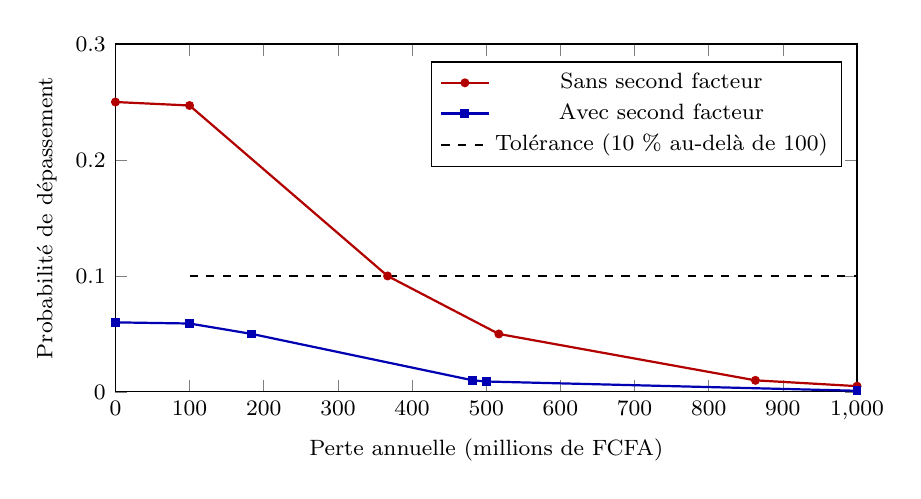
\begin{tikzpicture}
\begin{axis}[width=11cm, height=6cm, xmin=0, xmax=1000, ymin=0, ymax=0.3,
    xlabel={Perte annuelle (millions de FCFA)}, ylabel={Probabilité de dépassement},
    yticklabel style={/pgf/number format/fixed, /pgf/number format/precision=2},
    legend style={font=\footnotesize, at={(0.98,0.95)}, anchor=north east},
    tick label style={font=\footnotesize}, label style={font=\footnotesize}]
\addplot[thick, red!70!black, mark=*, mark size=1.2pt] coordinates
    {(0,0.25) (100,0.247) (367,0.10) (517,0.05) (863,0.01) (1000,0.005)};
\addplot[thick, blue!70!black, mark=square*, mark size=1.2pt] coordinates
    {(0,0.06) (100,0.059) (184,0.05) (482,0.01) (500,0.009) (1000,0.001)};
\addplot[thick, dashed, black] coordinates {(100,0.10) (1000,0.10)};
\legend{Sans second facteur, Avec second facteur, Tolérance (10~\% au-delà de 100)}
\end{axis}
\end{tikzpicture}
\end{center}
\vspace{-0.4em}
\begin{center}{\small\itshape Figure~10.1. Courbes de dépassement de R-02 (points issus du Tableau~10.2)}\end{center}

% ============================================================================
\section{L'Analyse de Sensibilité}
\label{sec:c10-sensibilite}
% ============================================================================

Quelles hypothèses comptent le plus~? On fait varier chacune entre ses
bornes plausibles, les autres restant fixes, et l'on observe la perte
annuelle moyenne.

\begin{tableaucours}{L{5.4cm}L{3.2cm}R{3.4cm}}{%
    \tableauHeader{Hypothèse (sans second facteur)} &
    \tableauHeader{Plage} &
    \tableauHeader{Perte moyenne}
}
Fréquence $\lambda$ & 0,20 à 0,40 & 65 à 130 \\
Médiane de la perte & 200 à 380 & 65 à 124 \\
\end{tableaucours}
\vspace{-0.8em}
\begin{center}{\small\itshape Tableau~10.3. Sensibilité de la perte moyenne (millions de FCFA)}\end{center}

\textbf{Analyse.} Les deux hypothèses pèsent autant. Mais la décision (le
second facteur) agit sur la fréquence, qu'elle divise par près de cinq~:
c'est elle qu'il faut vérifier en priorité, par l'indicateur de
couverture du second facteur. Une analyse de sensibilité dit où dépenser
l'effort de mesure.

\begin{boxmetier}{Gestionnaire de risques}
\textbf{Publier le code et les hypothèses.} Mme~MOUAFO conserve le
programme de simulation, les lois, les paramètres et la graine du tirage
aléatoire~: un tiers doit pouvoir refaire le calcul et obtenir les mêmes
chiffres.
\end{boxmetier}

\begin{boxmetier}{Auditeur des systèmes d'information}
\textbf{Refaire un point.} L'auditeur ne refait pas toute la simulation~;
il vérifie un résultat simple, par exemple que la moyenne est proche de
$\lambda \times$ perte moyenne ($0{,}29 \times 326 \approx 94$).
\end{boxmetier}

\separateur

\begin{boxresume}
\textbf{Ce qu'il faut retenir de ce chapitre~:}
\begin{itemize}
    \item \textbf{Monte-Carlo} tire des milliers d'années et en étudie la
          distribution.
    \item \textbf{Poisson} pour le nombre d'événements, \textbf{log-normale}
          pour l'ampleur.
    \item \textbf{Les centiles et la probabilité de dépassement} disent la
          pire année, que la moyenne cache.
    \item \textbf{La courbe de dépassement} se compare à la tolérance du
          conseil.
    \item \textbf{La sensibilité} dit quelles hypothèses vérifier d'abord.
\end{itemize}
\end{boxresume}

\begin{boxinfo}
\textbf{Points de contrôle de l'élève.} Je sais~: décrire les étapes d'une
simulation~; choisir les lois~; lire moyenne, centiles et probabilités de
dépassement~; vérifier une appétence en probabilité~; mener une analyse de
sensibilité.
\end{boxinfo}

\bigskip

\begin{boxexo}[title={\ding{45}\quad Exercice~10.1. Les étapes \niveaubase}]
Décrivez, en cinq lignes, ce que fait la simulation pour une seule année.
\end{boxexo}

\begin{boxexo}[title={\ding{45}\quad Exercice~10.2. Lire \niveaubase}]
D'après le Tableau~10.2, sans second facteur, combien d'années sur cent
dépassent 500~millions~?
\end{boxexo}

\begin{boxexo}[title={\ding{45}\quad Exercice~10.3. Poisson \niveaubase}]
Avec $\lambda = 0{,}29$, quelle est la probabilité d'une année sans aucun
événement~? Comparez au tableau.
\end{boxexo}

\begin{boxexo}[title={\ding{45}\quad Exercice~10.4. Le centile nul \niveaumoyen}]
Expliquez pourquoi le 90\textsuperscript{e} centile est nul avec second
facteur, alors que le 95\textsuperscript{e} atteint 184~millions.
\end{boxexo}

\begin{boxexo}[title={\ding{45}\quad Exercice~10.5. L'appétence \niveaumoyen}]
Montrez, à partir du Tableau~10.2, que l'appétence est respectée avec
second facteur et ne l'est pas sans.
\end{boxexo}

\begin{boxexo}[title={\ding{45}\quad Exercice~10.6. Vérifier la moyenne \niveaumoyen}]
Vérifiez que les moyennes du Tableau~10.2 sont cohérentes avec les
estimations FAIR du Chapitre~\ref{chap:quantitatif}.
\end{boxexo}

\begin{boxexo}[title={\ding{45}\quad Exercice~10.7. Pourquoi log-normale \niveaumoyen}]
Pourquoi une loi normale conviendrait-elle mal à l'ampleur d'une perte~?
\end{boxexo}

\begin{boxexo}[title={\ding{45}\quad Exercice~10.8. Sensibilité \niveaumoyen}]
Si la fréquence réelle sans second facteur était de 0,40, l'appétence
serait-elle encore plus loin d'être respectée~? Justifiez.
\end{boxexo}

\begin{boxexo}[title={\ding{45}\quad Exercice~10.9. Plusieurs risques \niveauexpert}]
Décrivez comment simuler ensemble les cinq risques numériques majeurs de
LiZbiZ pour vérifier l'appétence globale. Quelle difficulté pose leur
éventuelle dépendance~?
\end{boxexo}

\begin{boxexo}[title={\ding{45}\quad Exercice~10.10. Programmer \niveauexpert}]
Écrivez, en Python ou dans un tableur, une simulation de 10\,000 années
pour R-02 avec second facteur, et comparez vos résultats au
Tableau~10.2.
\end{boxexo}

\bigskip

\begin{boxinfo}
\textbf{Pour aller plus loin.}
\begin{itemize}
    \item IEC~31010, fiche sur la simulation de Monte-Carlo~\cite{iec31010}.
    \item D.~Hubbard et R.~Seiersen~\cite{hubbard2016cyber}.
\end{itemize}
\end{boxinfo}

\begin{boxinfo}
\textbf{Transition.} Estimer ne suffit pas~: il faut traiter, suivre et
rendre compte. C'est l'objet du Chapitre~\ref{chap:traiter}.
\end{boxinfo}
}{}
        \IfFileExists{partie2/P02_C11_traiter.tex}{% ============================================================================
% Fichier  : partie2/P02_C11_traiter.tex
% Titre    : Traiter, Suivre et Rendre Compte
% Auteur   : MINKA MI NGUIDJOÏ Thierry Emmanuel
% Version  : 1.0 -- novembre 2026
% ============================================================================
% Sources : ISO 31000:2018 (6.5 à 6.7) ; COSO ERM (2017) ; ISO/IEC 27005.
% Plan de traitement de LiZbiZ : cas fictif, montants cohérents entre eux.
% ============================================================================

\chapter{Traiter, Suivre et Rendre Compte}
\label{chap:traiter}
\chaptermark{Traiter, suivre, rendre compte}

\epigraph{%
    « Un risque n'est traité\\
    que lorsque la mesure fonctionne. »%
}{Principe du cours}

\niveauChapitre{Intermédiaire}{Chapitres~\ref{chap:gouvernance},
\ref{chap:matrices} et~\ref{chap:quantitatif}.}

\begin{boxobjectifs}
\begin{itemize}
    \item Choisir une option de traitement selon l'ISO~31000.
    \item Rédiger un plan de traitement complet.
    \item Arbitrer un budget par les pertes évitées.
    \item Définir des indicateurs clés de risque avec des seuils.
    \item Rendre compte au comité et au conseil.
\end{itemize}
\end{boxobjectifs}

\bigskip

% ============================================================================
\section*{Question directrice : comment dépenser les 180 millions votés en avril~?}
% ============================================================================

En avril, sous le choc, le comité de direction a voté 180~millions de
FCFA pour la sécurité. En juin, le registre et les estimations sont
prêts. Il reste à choisir les traitements, à les confier à des
responsables, et à savoir, chaque trimestre, si le risque baisse
vraiment.

\medskip
\textbf{Plan du chapitre.}
\begin{enumerate}
    \item Les options de traitement (section~\ref{sec:c11-options}).
    \item Le plan de traitement (section~\ref{sec:c11-plan}).
    \item Arbitrer le budget (section~\ref{sec:c11-budget}).
    \item Les indicateurs clés de risque (section~\ref{sec:c11-kri}).
    \item Rendre compte (section~\ref{sec:c11-rendre}).
\end{enumerate}

\separateur

% ============================================================================
\section{Les Options de Traitement}
\label{sec:c11-options}
% ============================================================================

L'ISO~31000 énumère plusieurs options, qui se combinent~\cite{iso31000_2018}.

\begin{tableaucours}{L{3.6cm}L{4.6cm}L{4.0cm}}{%
    \tableauHeader{Option} &
    \tableauHeader{Principe} &
    \tableauHeader{Exemple chez LiZbiZ}
}
Éviter & Renoncer à l'activité qui crée le risque & Supprimer l'accès
distant permanent du prestataire \\
Retirer la source & Supprimer la cause & Remplacer FTP par SFTP \\
Modifier la vraisemblance & Rendre l'événement moins probable & Second
facteur, correctifs \\
Modifier les conséquences & Limiter les dommages & Sauvegardes hors ligne,
mode dégradé \\
Partager & Transférer une part des conséquences & Assurance cyber, clauses
du contrat \\
Maintenir & Accepter en connaissance de cause, par écrit & Défiguration du
portail, sous surveillance \\
Prendre le risque & Saisir une opportunité & Ouvrir un portail client en
ligne, avec ses mesures \\
\end{tableaucours}
\vspace{-0.8em}
\begin{center}{\small\itshape Tableau~11.1. Les options de traitement (d'après l'ISO 31000:2018)}\end{center}

\begin{boxalert}
\textbf{Violation typique.} Croire que l'assurance « traite » le risque.

\smallskip
\textbf{Règle~:} l'assurance partage une part des pertes financières~;
elle ne réduit ni la vraisemblance, ni l'arrêt de l'activité, ni l'atteinte
aux clients. Elle complète la réduction, elle ne la remplace pas. Et
l'assureur exige souvent, en contrepartie, des mesures (second facteur,
sauvegardes).
\end{boxalert}

% ============================================================================
\section{Le Plan de Traitement}
\label{sec:c11-plan}
% ============================================================================

\begin{boxdef}
\termecle{Plan de traitement}~: document qui précise, pour chaque risque
traité, les actions retenues, leur justification, le responsable, les
ressources, l'échéance, l'indicateur de suivi et le risque résiduel visé.
\end{boxdef}

\begin{tableaucours}{L{1.0cm}L{4.2cm}L{2.2cm}L{1.6cm}L{2.8cm}}{%
    \tableauHeader{Risque} &
    \tableauHeader{Action} &
    \tableauHeader{Responsable} &
    \tableauHeader{Échéance} &
    \tableauHeader{Indicateur}
}
R-02 & Second facteur sur la passerelle & M.~KOUNOU & Juillet & Part des
connexions avec second facteur \\
R-02 & Bastion d'administration & M.~KOUNOU & Septembre & Part des accès
du prestataire par le bastion \\
R-01 & Sauvegardes hors ligne et immuables & M.~KOUNOU & Août & Durée du
dernier test de restauration \\
R-07 & Chiffrement des bases clients & M.~KOUNOU & Octobre & Part des
bases chiffrées \\
R-11 & Rayonnages surélevés et pompes & M.~NGUELE & Septembre & Hauteur
des stocks au sol \\
R-03 & Second lien télécom à Garoua & M.~NGUELE & Novembre & Durée des
coupures \\
\end{tableaucours}
\vspace{-0.8em}
\begin{center}{\small\itshape Tableau~11.2. Extrait du plan de traitement de LiZbiZ}\end{center}

Le \termecle{risque résiduel} est réévalué avec les seules mesures en place
et vérifiées~; il est \emph{accepté par écrit} par le propriétaire et, au
besoin, par la direction. Une mesure décidée mais non mise en œuvre ne
réduit rien (cours SEC3266, Chapitre sur les risques).

% ============================================================================
\section{Arbitrer le Budget}
\label{sec:c11-budget}
% ============================================================================

On classe les traitements par \emph{pertes annuelles évitées nettes} et par
rapport au coût annuel. Les pertes évitées viennent des estimations FAIR
(Chapitre~\ref{chap:quantitatif}) pour les risques majeurs, et d'ordres de
grandeur pour les autres.

\begin{tableaucours}{L{4.8cm}R{1.8cm}R{2.2cm}R{2.4cm}}{%
    \tableauHeader{Traitement} &
    \tableauHeader{Coût annuel} &
    \tableauHeader{Pertes évitées} &
    \tableauHeader{Rapport net}
}
Second facteur (R-02) & 6 & 74 & 11,3 \\
Sauvegardes hors ligne (R-01) & 15 & 60 & 3,0 \\
Bastion (R-02) & 10 & 25 & 1,5 \\
Rayonnages et pompes (R-11) & 4 & 9 & 1,3 \\
Surveillance externalisée (SOC) & 60 & 45 & -0,25 \\
\end{tableaucours}
\vspace{-0.8em}
\begin{center}{\small\itshape Tableau~11.3. Arbitrage des traitements (millions de FCFA par an ; rapport = (évité moins coût) / coût)}\end{center}

\begin{boxscenario}{Opération LIZBIZ. La décision de juin}
\textbf{Constatation.} Les quatre premiers traitements coûtent 35~millions
par an et évitent environ 168~millions de pertes attendues. La
surveillance externalisée coûte plus qu'elle n'évite, selon les
estimations.

\medskip
\textbf{Analyse} (confiance faible). La surveillance réduit surtout le
délai de détection, dont l'effet sur les pertes est mal estimé~; le
rapport négatif peut venir de cette sous-estimation. Le comité retient les
quatre premiers traitements, et une surveillance limitée aux heures de
nuit, à réévaluer après six mois de mesures.
\end{boxscenario}

% ============================================================================
\section{Les Indicateurs Clés de Risque}
\label{sec:c11-kri}
% ============================================================================

\begin{boxdef}
\termecle{Indicateur clé de risque} (KRI)~: mesure qui signale à l'avance
l'évolution d'un risque, assortie de seuils d'alerte. Il se distingue de
l'indicateur de performance, qui mesure l'atteinte d'un objectif.
\end{boxdef}

\begin{tableaucours}{L{4.8cm}L{1.0cm}L{2.0cm}L{2.0cm}L{2.0cm}}{%
    \tableauHeader{Indicateur} &
    \tableauHeader{Risque} &
    \tableauHeader{Vert} &
    \tableauHeader{Orange} &
    \tableauHeader{Rouge}
}
Connexions distantes avec second facteur & R-02 & 100~\% & 95 à 99~\% &
moins de 95~\% \\
Âge du dernier test de restauration réussi & R-01 & moins de 3~mois & 3 à
6~mois & plus de 6~mois \\
Correctifs critiques en retard & R-02 & 0 & 1 à 3 & plus de 3 \\
Comptes orphelins actifs & R-07 & 0 & 1 à 5 & plus de 5 \\
\end{tableaucours}
\vspace{-0.8em}
\begin{center}{\small\itshape Tableau~11.4. Indicateurs clés de risque de LiZbiZ}\end{center}

Un bon indicateur clé de risque est \emph{avancé} (il bouge avant
l'incident), \emph{mesurable} automatiquement si possible, et rattaché à un
\emph{propriétaire} qui agit quand il passe à l'orange.

% ============================================================================
\section{Rendre Compte}
\label{sec:c11-rendre}
% ============================================================================

\begin{boxprocedure}
\textbf{Le rapport trimestriel au comité des risques}
\begin{enumerate}
    \item Les dix premiers risques, avec leur score et leur évolution
          depuis le trimestre précédent.
    \item L'avancement du plan de traitement~: actions faites, en retard,
          bloquées.
    \item Les indicateurs clés de risque passés à l'orange ou au rouge, et
          ce qui a été fait.
    \item Les incidents du trimestre et les risques qu'ils révèlent.
    \item Les risques nouveaux ou émergents.
    \item Les décisions demandées au comité.
\end{enumerate}
\end{boxprocedure}

\begin{boxobjet}{R-01 · Arrêt de la facturation (suivi)}
\textbf{Cotation~:} V=3, I=3 (score~9) en juin~; cible V=2, I=2 après
sauvegardes testées et mode dégradé. \textbf{Traitement~:} sauvegardes hors
ligne (août), test trimestriel. \textbf{Propriétaire~:} Mme~MBALLA.
\textbf{Indicateur~:} âge du dernier test de restauration réussi (vert sous
trois mois).
\end{boxobjet}

\begin{boxmetier}{Gestionnaire de risques}
\textbf{Une page pour le conseil.} Le conseil reçoit chaque semestre une
seule page~: respect de l'appétence, les cinq risques majeurs, les
décisions qui lui reviennent. Le détail est en annexe.
\end{boxmetier}

\separateur

\begin{boxresume}
\textbf{Ce qu'il faut retenir de ce chapitre~:}
\begin{itemize}
    \item \textbf{Plusieurs options} se combinent~; l'assurance partage,
          elle ne réduit pas.
    \item \textbf{Le plan de traitement} nomme l'action, le responsable,
          l'échéance, l'indicateur et le résiduel visé.
    \item \textbf{On arbitre} par les pertes évitées nettes, en disant la
          confiance de l'estimation.
    \item \textbf{Les indicateurs clés de risque} sont avancés, mesurables,
          à seuils, et ont un propriétaire.
    \item \textbf{Rendre compte}~: dix risques, plan, indicateurs,
          incidents, émergents, décisions.
\end{itemize}
\end{boxresume}

\begin{boxinfo}
\textbf{Points de contrôle de l'élève.} Je sais~: choisir une option de
traitement~; rédiger une ligne de plan de traitement~; calculer un rapport
net~; définir un indicateur clé de risque et ses seuils~; structurer un
rapport trimestriel.
\end{boxinfo}

\bigskip

\begin{boxexo}[title={\ding{45}\quad Exercice~11.1. Quelle option~? \niveaubase}]
Donnez l'option de traitement~: souscrire une assurance~; fermer l'agence
de Garoua~; installer des pompes à Bonabéri~; accepter la défiguration du
portail.
\end{boxexo}

\begin{boxexo}[title={\ding{45}\quad Exercice~11.2. Rapport net \niveaubase}]
Un traitement coûte 8~millions par an et évite 20~millions de pertes
attendues. Calculez le rapport net.
\end{boxexo}

\begin{boxexo}[title={\ding{45}\quad Exercice~11.3. KRI ou KPI \niveaubase}]
Classez en indicateur clé de risque ou de performance~: le chiffre
d'affaires mensuel~; le nombre de correctifs critiques en retard~; le taux
de livraison à l'heure.
\end{boxexo}

\begin{boxexo}[title={\ding{45}\quad Exercice~11.4. L'assurance \niveaumoyen}]
Pourquoi l'assurance seule ne suffit-elle pas pour R-02~? Que demandera
probablement l'assureur à LiZbiZ~?
\end{boxexo}

\begin{boxexo}[title={\ding{45}\quad Exercice~11.5. Une ligne de plan \niveaumoyen}]
Rédigez la ligne du plan de traitement pour le chiffrement des
ordinateurs portables de la direction.
\end{boxexo}

\begin{boxexo}[title={\ding{45}\quad Exercice~11.6. Le budget \niveaumoyen}]
Sur les 180~millions votés, combien restent après les quatre premiers
traitements du Tableau~11.3 la première année~? Que proposez-vous d'en
faire~?
\end{boxexo}

\begin{boxexo}[title={\ding{45}\quad Exercice~11.7. Le SOC \niveaumoyen}]
Le rapport net de la surveillance externalisée est négatif. Quelles
pertes évitées l'estimation a-t-elle pu oublier~?
\end{boxexo}

\begin{boxexo}[title={\ding{45}\quad Exercice~11.8. Seuils \niveaumoyen}]
Proposez des seuils vert, orange et rouge pour l'indicateur « hauteur des
marchandises stockées au sol à Bonabéri en saison des pluies ».
\end{boxexo}

\begin{boxexo}[title={\ding{45}\quad Exercice~11.9. Le rapport \niveauexpert}]
Rédigez le rapport trimestriel de septembre au comité des risques de
LiZbiZ, à partir des éléments du chapitre.
\end{boxexo}

\begin{boxexo}[title={\ding{45}\quad Exercice~11.10. La page du conseil \niveauexpert}]
Rédigez la page semestrielle au conseil~: appétence, cinq risques majeurs,
décisions demandées.
\end{boxexo}

\bigskip

\begin{boxinfo}
\textbf{Pour aller plus loin.}
\begin{itemize}
    \item ISO~31000, traitement, suivi et rapport~\cite{iso31000_2018}.
    \item COSO ERM~\cite{coso2017erm}.
\end{itemize}
\end{boxinfo}

\begin{boxinfo}
\textbf{Transition.} Un dispositif de risques se vérifie. La Partie~III
apprend à l'auditer, en commençant par l'ISO~19011
(Chapitre~\ref{chap:audit}).
\end{boxinfo}
}{}

    \part{Auditer le Dispositif}
    \label{part:audit}

        \IfFileExists{partie3/P03_C12_audit.tex}{% ============================================================================
% Fichier  : partie3/P03_C12_audit.tex
% Titre    : L'Audit selon l'ISO 19011
% Auteur   : MINKA MI NGUIDJOÏ Thierry Emmanuel
% Version  : 1.0 -- novembre 2026
% ============================================================================
% Sources : ISO 19011:2018 ; ISO/IEC 27007:2020 ; loi n° 2010/012 (art. 13 et
% 32, cités au chapitre 5). Programme d'audit de LiZbiZ : cas fictif.
% ============================================================================

\chapter{L'Audit selon l'ISO 19011}
\label{chap:audit}
\chaptermark{L'audit selon l'ISO 19011}

\epigraph{%
    « Auditer, ce n'est pas chercher des fautes~;\\
    c'est établir, preuves à l'appui, ce qui fonctionne et ce qui manque. »%
}{Principe du cours}

\niveauChapitre{Intermédiaire}{Chapitres~\ref{chap:gouvernance},
\ref{chap:droit} et~\ref{chap:traiter}~; cours INF3226.}

\begin{boxobjectifs}
\begin{itemize}
    \item Distinguer les audits de première, deuxième et troisième partie.
    \item Énoncer les sept principes de l'audit de l'ISO~19011.
    \item Établir un programme d'audit fondé sur les risques.
    \item Définir les rôles d'une équipe d'audit et les compétences
          attendues.
    \item Situer l'ISO/IEC~27007 pour l'audit d'un système de management de
          la sécurité.
\end{itemize}
\end{boxobjectifs}

\bigskip

% ============================================================================
\section*{Question directrice : que fallait-il auditer, et quand, chez LiZbiZ~?}
% ============================================================================

Le dernier audit de sécurité de LiZbiZ datait de 2023 et ne couvrait pas
le prestataire. Au printemps 2026, la mission d'AUDIX CONSEIL a examiné
cinq domaines du système d'information (cours INF3226). En septembre, le
comité d'audit demande à Mme~NKENG un \emph{programme} d'audit sur deux
ans, qui couvre en priorité ce qui présente le plus de risques, y compris
le dispositif de gestion des risques lui-même.

\medskip
\textbf{Plan du chapitre.}
\begin{enumerate}
    \item Les types d'audit (section~\ref{sec:c12-types}).
    \item Les principes de l'audit (section~\ref{sec:c12-principes}).
    \item Le programme d'audit (section~\ref{sec:c12-programme}).
    \item Les rôles et les compétences (section~\ref{sec:c12-roles}).
    \item L'audit d'un système de management de la sécurité (section~\ref{sec:c12-27007}).
\end{enumerate}

\separateur

% ============================================================================
\section{Les Types d'Audit}
\label{sec:c12-types}
% ============================================================================

\begin{boxdef}
\termecle{Audit} (ISO~19011)~: processus méthodique, indépendant et
documenté, permettant d'obtenir des preuves objectives et de les évaluer de
manière objective pour déterminer dans quelle mesure les critères d'audit
sont satisfaits~\cite{iso19011_2018}.
\end{boxdef}

\begin{tableaucours}{L{3.2cm}L{4.4cm}L{4.6cm}}{%
    \tableauHeader{Type} &
    \tableauHeader{Qui audite} &
    \tableauHeader{Exemple}
}
Première partie & L'organisation elle-même (audit interne) & Mme~NKENG
audite le dispositif de risques \\
Deuxième partie & Un client ou un donneur d'ordre & LiZbiZ audite SAHEL
INFOGÉRANCE, selon la clause du contrat \\
Troisième partie & Un organisme indépendant & Certification ISO/IEC~27001~;
audit de l'Agence au titre de l'article~32 \\
\end{tableaucours}
\vspace{-0.8em}
\begin{center}{\small\itshape Tableau~12.1. Les trois types d'audit}\end{center}

Les \termecle{critères d'audit} sont le référentiel auquel on compare les
preuves~: une norme, une politique interne, une clause de contrat, un
article de loi. Sans critère, il n'y a pas d'écart, seulement des opinions.

% ============================================================================
\section{Les Principes de l'Audit}
\label{sec:c12-principes}
% ============================================================================

\begin{tableaucours}{L{4.2cm}L{8.0cm}}{%
    \tableauHeader{Principe} &
    \tableauHeader{Ce qu'il exige}
}
Intégrité & Honnêteté, diligence, respect de la loi, impartialité \\
Présentation impartiale & Rapporter fidèlement, y compris les désaccords
non résolus \\
Conscience professionnelle & Diligence et jugement proportionnés à
l'importance de la tâche \\
Confidentialité & Protéger les informations obtenues \\
Indépendance & Ne pas auditer son propre travail~; rester libre de tout
conflit d'intérêts \\
Approche fondée sur la preuve & Des conclusions vérifiables, fondées sur un
échantillon d'informations disponibles \\
Approche fondée sur le risque & Concentrer l'audit sur ce qui compte pour
l'organisation et pour l'atteinte des objectifs de l'audit \\
\end{tableaucours}
\vspace{-0.8em}
\begin{center}{\small\itshape Tableau~12.2. Les sept principes de l'audit (ISO 19011:2018)}\end{center}

\begin{boxalert}
\textbf{Violation typique.} Confier l'audit du dispositif de risques à la
personne qui l'a conçu.

\smallskip
\textbf{Règle~:} Mme~MOUAFO ne peut pas auditer le registre qu'elle tient~;
Mme~NKENG le peut, parce qu'elle n'y a pas pris part
(Chapitre~\ref{chap:gouvernance}). Si l'auditeur a conseillé la
conception, il le déclare et l'on confie le sujet à un autre.
\end{boxalert}

% ============================================================================
\section{Le Programme d'Audit}
\label{sec:c12-programme}
% ============================================================================

\begin{boxdef}
\termecle{Programme d'audit}~: ensemble d'un ou plusieurs audits planifiés
pour une durée donnée et dirigés vers un but spécifique. Il précise les
objectifs, les risques et opportunités du programme, l'étendue, les
ressources, le calendrier et la manière de le surveiller.
\end{boxdef}

Un programme fondé sur les risques consacre plus d'audits, et plus tôt,
aux processus les plus exposés, en s'appuyant sur le registre des risques
(Chapitre~\ref{chap:matrices}).

\begin{tableaucours}{L{4.4cm}L{2.0cm}L{2.6cm}L{3.0cm}}{%
    \tableauHeader{Audit} &
    \tableauHeader{Risques} &
    \tableauHeader{Période} &
    \tableauHeader{Type}
}
Accès distants et prestataire & R-02 & Octobre 2026 & 1\textsuperscript{re}
et 2\textsuperscript{e} partie \\
Dispositif de gestion des risques & Tous & Octobre 2026 & 1\textsuperscript{re}
partie \\
Sauvegardes et reprise & R-01 & Janvier 2027 & 1\textsuperscript{re} partie \\
Données personnelles & R-07 & Mars 2027 & 1\textsuperscript{re} partie,
avec conseil \\
Continuité des agences & R-03, R-11 & Juin 2027 & 1\textsuperscript{re}
partie \\
Préparation à la certification ISO/IEC~27001 & SMSI & Septembre 2027 &
Audit à blanc \\
\end{tableaucours}
\vspace{-0.8em}
\begin{center}{\small\itshape Tableau~12.3. Programme d'audit 2026-2027 de LiZbiZ}\end{center}

\begin{boxscenario}{Opération LIZBIZ. Le programme validé}
\textbf{Constatation.} Le comité d'audit valide le programme le
30~septembre. Le premier audit, « accès distants et prestataire », combine
un audit interne et l'audit de SAHEL INFOGÉRANCE prévu par la nouvelle
clause du contrat.

\medskip
\textbf{Analyse} (confiance élevée). Le programme suit l'ordre des risques
du registre~: c'est l'approche fondée sur le risque. Il prévoit en outre
d'auditer le dispositif de risques lui-même, sans quoi un registre faux
orienterait faussement tout le programme.
\end{boxscenario}

% ============================================================================
\section{Les Rôles et les Compétences}
\label{sec:c12-roles}
% ============================================================================

\begin{tableaucours}{L{4.0cm}L{8.2cm}}{%
    \tableauHeader{Rôle} &
    \tableauHeader{Responsabilité}
}
Responsable du programme & Établit, met en œuvre, surveille et améliore le
programme \\
Responsable de l'équipe d'audit & Prépare et conduit un audit, répartit les
tâches, rédige le rapport \\
Auditeur & Recueille et évalue les preuves, rédige les constats \\
Expert technique & Apporte une compétence particulière, sous la
responsabilité d'un auditeur \\
Guide et observateur & Accompagnent l'équipe sans participer à
l'évaluation \\
\end{tableaucours}
\vspace{-0.8em}
\begin{center}{\small\itshape Tableau~12.4. Les rôles d'un audit}\end{center}

L'ISO~19011 décrit les compétences de l'auditeur~: comportement
professionnel (éthique, ouverture, observation, ténacité), connaissances
génériques (principes, méthodes, systèmes de management) et connaissances
propres à la discipline (ici, les risques et la sécurité de l'information).

% ============================================================================
\section{L'Audit d'un Système de Management de la Sécurité}
\label{sec:c12-27007}
% ============================================================================

L'\norme{ISO/IEC~27007:2020} complète l'ISO~19011 pour l'audit d'un système
de management de la sécurité de l'information~\cite{iso27007_2020}. Elle
précise ce qu'il faut examiner aux clauses~4 à~10 de l'ISO/IEC~27001
(contexte, leadership, planification dont l'appréciation des risques,
support, fonctionnement, évaluation, amélioration) et comment relier les
mesures de l'annexe~A aux risques.

\begin{boxobjet}{R-02 · Point d'audit}
\textbf{Scénario audité~:} usurpation de l'accès distant du prestataire.
\textbf{Critères~:} politique d'accès distant, clause du contrat
(octobre 2026), article~29, alinéa~2 de la loi n°~2010/012.
\textbf{Preuves attendues~:} configuration de la passerelle, journaux de
connexion, liste des comptes du prestataire, procès-verbal de l'audit du
prestataire. \textbf{Propriétaire~:} M.~NGUELE.
\end{boxobjet}

\begin{boxmetier}{Auditeur des systèmes d'information}
\textbf{Écrire les critères avant d'arriver.} L'auditeur liste, avant la
réunion d'ouverture, chaque critère et la preuve qui permettra de dire s'il
est satisfait. Ce qu'il ne peut pas relier à un critère n'ira pas dans le
rapport comme écart.
\end{boxmetier}

\separateur

\begin{boxresume}
\textbf{Ce qu'il faut retenir de ce chapitre~:}
\begin{itemize}
    \item \textbf{L'audit} compare des preuves objectives à des critères~;
          il est interne, de deuxième ou de troisième partie.
    \item \textbf{Sept principes}, dont l'indépendance, l'approche fondée
          sur la preuve et l'approche fondée sur le risque.
    \item \textbf{Le programme} suit le registre des risques et audite aussi
          le dispositif de risques.
    \item \textbf{Les rôles} sont distincts~; l'expert technique travaille
          sous la responsabilité d'un auditeur.
    \item \textbf{L'ISO/IEC~27007} adapte l'ISO~19011 au système de
          management de la sécurité.
\end{itemize}
\end{boxresume}

\begin{boxinfo}
\textbf{Points de contrôle de l'élève.} Je sais~: définir l'audit et les
critères d'audit~; distinguer les trois types~; citer les sept principes~;
construire un programme fondé sur les risques~; situer l'ISO/IEC~27007.
\end{boxinfo}

\bigskip

\begin{boxexo}[title={\ding{45}\quad Exercice~12.1. Quel type~? \niveaubase}]
Classez~: l'audit de LiZbiZ par son assureur~; l'audit de la paie par
Mme~NKENG~; l'audit de certification par un organisme accrédité.
\end{boxexo}

\begin{boxexo}[title={\ding{45}\quad Exercice~12.2. Les critères \niveaubase}]
Donnez trois critères d'audit possibles pour l'audit « sauvegardes et
reprise ».
\end{boxexo}

\begin{boxexo}[title={\ding{45}\quad Exercice~12.3. Principes \niveaubase}]
Quel principe un auditeur viole-t-il en omettant du rapport un désaccord
avec l'audité~?
\end{boxexo}

\begin{boxexo}[title={\ding{45}\quad Exercice~12.4. Indépendance \niveaumoyen}]
M.~KOUNOU propose d'auditer lui-même les sauvegardes, qu'il connaît
mieux que quiconque. Que répondez-vous~? Comment utiliser sa compétence~?
\end{boxexo}

\begin{boxexo}[title={\ding{45}\quad Exercice~12.5. Fondé sur le risque \niveaumoyen}]
Justifiez l'ordre du programme du Tableau~12.3 par le registre des risques
du Chapitre~\ref{chap:matrices}.
\end{boxexo}

\begin{boxexo}[title={\ding{45}\quad Exercice~12.6. Le prestataire \niveaumoyen}]
Quelles conditions doit réunir l'audit de SAHEL INFOGÉRANCE par LiZbiZ
pour être possible et utile~?
\end{boxexo}

\begin{boxexo}[title={\ding{45}\quad Exercice~12.7. L'expert \niveaumoyen}]
AUDIX CONSEIL fournit un expert des passerelles d'accès distant. Quel est
son rôle, et qui signe les constats~?
\end{boxexo}

\begin{boxexo}[title={\ding{45}\quad Exercice~12.8. Les risques du programme \niveaumoyen}]
Citez trois risques qui menacent le programme d'audit lui-même, et une
parade pour chacun.
\end{boxexo}

\begin{boxexo}[title={\ding{45}\quad Exercice~12.9. Un programme bancaire \niveauexpert}]
Construisez le programme d'audit sur deux ans de la BANQUE SANAGA,
fondé sur ses risques.
\end{boxexo}

\begin{boxexo}[title={\ding{45}\quad Exercice~12.10. Clauses 4 à 10 \niveauexpert}]
Pour chaque clause de 4 à 10 de l'ISO/IEC~27001, donnez une preuve que
l'auditeur demandera à LiZbiZ.
\end{boxexo}

\bigskip

\begin{boxinfo}
\textbf{Pour aller plus loin.}
\begin{itemize}
    \item ISO~19011~\cite{iso19011_2018}~; ISO/IEC~27007~\cite{iso27007_2020}.
\end{itemize}
\end{boxinfo}

\begin{boxinfo}
\textbf{Transition.} Le programme posé, il faut conduire chaque audit. Le
Chapitre~\ref{chap:conduire} traite des preuves, des échantillons et des
constats.
\end{boxinfo}
}{}
        \IfFileExists{partie3/P03_C13_conduire.tex}{% ============================================================================
% Fichier  : partie3/P03_C13_conduire.tex
% Titre    : Conduire l'Audit : Preuves, Échantillons, Constats
% Auteur   : MINKA MI NGUIDJOÏ Thierry Emmanuel
% Version  : 1.0 -- novembre 2026
% ============================================================================
% Sources : ISO 19011:2018 (6.3 à 6.4, annexe A) ; ISO/IEC 27007:2020.
% Tailles d'échantillon et limites supérieures : loi binomiale, confiance
% 95 %, calculées et vérifiées. Audit d'octobre 2026 : cas fictif.
% ============================================================================

\chapter{Conduire l'Audit : Preuves, Échantillons, Constats}
\label{chap:conduire}
\chaptermark{Preuves, échantillons, constats}

\epigraph{%
    « Zéro anomalie dans un échantillon\\
    ne veut pas dire zéro anomalie dans la population. »%
}{Principe du cours}

\niveauChapitre{Intermédiaire à expert}{Chapitre~\ref{chap:audit}~;
notions de probabilité.}

\begin{boxobjectifs}
\begin{itemize}
    \item Dérouler les étapes d'un audit, de la préparation à la réunion de
          clôture.
    \item Juger la force d'une preuve selon sa source.
    \item Dimensionner un échantillon par attributs et en tirer une limite
          supérieure d'anomalies.
    \item Rédiger un constat~: critère, fait, preuve, cause, conséquence.
    \item Distinguer non-conformité, opportunité d'amélioration et
          conformité.
\end{itemize}
\end{boxobjectifs}

\bigskip

% ============================================================================
\section*{Question directrice : 29 connexions examinées suffisent-elles à conclure sur 1 340~?}
% ============================================================================

En octobre, Mme~NKENG audite les accès distants de LiZbiZ. En septembre,
la passerelle a enregistré 1\,340~connexions. Elle ne peut pas les examiner
toutes à la main. Combien en examiner, comment les choisir, et que
conclure si elle trouve une ou deux connexions sans second facteur~?

\medskip
\textbf{Plan du chapitre.}
\begin{enumerate}
    \item Les étapes d'un audit (section~\ref{sec:c13-etapes}).
    \item Les preuves (section~\ref{sec:c13-preuves}).
    \item Échantillonner (section~\ref{sec:c13-echantillon}).
    \item Conclure sur la population (section~\ref{sec:c13-conclure}).
    \item Rédiger un constat (section~\ref{sec:c13-constat}).
\end{enumerate}

\separateur

% ============================================================================
\section{Les Étapes d'un Audit}
\label{sec:c13-etapes}
% ============================================================================

\begin{tableaucours}{L{3.6cm}L{8.6cm}}{%
    \tableauHeader{Étape} &
    \tableauHeader{Contenu (d'après l'ISO 19011:2018)}
}
Déclenchement & Contact avec l'audité, faisabilité, accès aux informations \\
Préparation & Revue documentaire, plan d'audit, répartition des tâches,
documents de travail (listes de vérification, plans d'échantillonnage) \\
Réunion d'ouverture & Confirmer le périmètre, les critères, le
calendrier, les modalités \\
Collecte et vérification & Entretiens, observations, examen de documents et
d'enregistrements, essais \\
Constats & Comparer les preuves aux critères \\
Conclusions & Synthèse des constats au regard des objectifs de l'audit \\
Réunion de clôture & Présenter constats et conclusions, recueillir les
désaccords \\
Rapport et suivi & Rapport, actions correctives, vérification
(Chapitre~\ref{chap:rapport}) \\
\end{tableaucours}
\vspace{-0.8em}
\begin{center}{\small\itshape Tableau~13.1. Les étapes d'un audit}\end{center}

% ============================================================================
\section{Les Preuves}
\label{sec:c13-preuves}
% ============================================================================

\begin{boxdef}
\termecle{Preuve d'audit}~: enregistrements, énoncés de faits ou autres
informations, pertinents pour les critères d'audit et vérifiables.
\end{boxdef}

\begin{tableaucours}{L{3.4cm}L{2.2cm}L{6.6cm}}{%
    \tableauHeader{Source} &
    \tableauHeader{Force} &
    \tableauHeader{Exemple}
}
Essai refait par l'auditeur & Élevée & Tenter une connexion à la passerelle
sans second facteur \\
Enregistrement produit par le système & Élevée & Journal de la passerelle,
exporté en présence de l'auditeur, avec son empreinte \\
Document & Moyenne & Politique d'accès distant signée \\
Observation & Moyenne & Voir le technicien se connecter par le bastion \\
Déclaration & Faible & « Tout le monde a le second facteur depuis juillet » \\
\end{tableaucours}
\vspace{-0.8em}
\begin{center}{\small\itshape Tableau~13.2. Force des preuves selon leur source}\end{center}

\begin{boxalert}
\textbf{Violation typique.} Conclure sur une déclaration.

\smallskip
\textbf{Règle~:} une déclaration oriente la recherche, elle ne prouve pas.
On la corrobore par un enregistrement ou un essai. Faute de corroboration,
le point reste ouvert (au Chapitre~\ref{chap:retex}, on le cotera \NEK{}).
\end{boxalert}

% ============================================================================
\section{Échantillonner}
\label{sec:c13-echantillon}
% ============================================================================

Quand la population est trop grande, l'auditeur examine un
\termecle{échantillon}. Il peut le choisir \emph{par jugement} (les
connexions de nuit, celles du prestataire) ou \emph{statistiquement}
(au hasard), ce qui seul permet d'étendre une conclusion chiffrée à la
population.

\begin{boxdef}
\termecle{Échantillonnage par attributs}~: on compte, dans un échantillon
tiré au hasard, les éléments qui présentent une anomalie (oui ou non). On
fixe un \emph{taux tolérable} d'anomalies et un \emph{niveau de confiance}.
\end{boxdef}

Si l'on s'attend à ne trouver aucune anomalie, la taille minimale $n$ pour
conclure, avec une confiance de 95~\%, que le taux d'anomalies est
inférieur au taux tolérable $t$ vérifie $(1 - t)^n \le 0{,}05$~:
\[
n \ge \frac{\ln 0{,}05}{\ln(1 - t)}.
\]

\begin{tableaucours}{L{4.0cm}R{3.0cm}}{%
    \tableauHeader{Taux tolérable} &
    \tableauHeader{Taille minimale}
}
10~\% & 29 \\
5~\% & 59 \\
3~\% & 99 \\
\end{tableaucours}
\vspace{-0.8em}
\begin{center}{\small\itshape Tableau~13.3. Tailles d'échantillon, confiance 95~\%, aucune anomalie attendue}\end{center}

La taille dépend du taux tolérable et de la confiance, presque pas de la
taille de la population, dès que celle-ci est grande. 29 connexions
suffisent pour 1\,340 comme pour 100\,000.

% ============================================================================
\section{Conclure sur la Population}
\label{sec:c13-conclure}
% ============================================================================

Si l'échantillon contient des anomalies, on calcule la \termecle{limite
supérieure} du taux d'anomalies dans la population, à 95~\% de confiance.

\begin{tableaucours}{L{3.6cm}R{2.8cm}R{2.8cm}}{%
    \tableauHeader{Anomalies trouvées} &
    \tableauHeader{Échantillon de 29} &
    \tableauHeader{Échantillon de 59}
}
0 & 9,8~\% & 5,0~\% \\
1 & 15,3~\% & 7,8~\% \\
2 & 20,2~\% & 10,3~\% \\
\end{tableaucours}
\vspace{-0.8em}
\begin{center}{\small\itshape Tableau~13.4. Limite supérieure du taux d'anomalies, confiance 95~\%}\end{center}

\begin{boxscenario}{Opération LIZBIZ. Les connexions de septembre}
\textbf{Constatation.} Sur 29~connexions tirées au hasard parmi 1\,340,
une s'est faite sans second facteur, par le compte « vpn\_secours »,
exclu de la politique pour « dépannage ». L'essai de l'auditrice confirme
que ce compte se connecte avec son seul mot de passe.

\medskip
\textbf{Analyse} (confiance élevée). Avec une anomalie sur 29, le taux
réel peut atteindre 15,3~\%~: on ne peut pas conclure que 90~\% au moins
des connexions ont un second facteur. Mais l'enjeu n'est plus statistique~:
la cause est identifiée (un compte exclu), et toutes les connexions de ce
compte sont à examiner, par un test exhaustif ciblé.
\end{boxscenario}

% ============================================================================
\section{Rédiger un Constat}
\label{sec:c13-constat}
% ============================================================================

\begin{boxprocedure}
\textbf{Les éléments d'un constat}
\begin{enumerate}
    \item \textbf{Critère}~: l'exigence (politique, clause, article).
    \item \textbf{Constat}~: le fait observé, chiffré.
    \item \textbf{Preuve}~: la pièce qui l'établit, avec sa référence.
    \item \textbf{Cause}~: pourquoi l'écart existe.
    \item \textbf{Conséquence}~: le risque qui en résulte, relié au registre.
    \item \textbf{Classement}~: non-conformité (majeure ou mineure),
          opportunité d'amélioration, ou conformité.
\end{enumerate}
\end{boxprocedure}

\begin{boxobjet}{Constat A-03 · Compte d'accès distant sans second facteur}
\textbf{Critère~:} politique d'accès distant (juillet 2026)~: « toute
connexion distante exige un second facteur ». \textbf{Constat~:} le compte
« vpn\_secours » se connecte sans second facteur~; 46~connexions en
septembre. \textbf{Preuve~:} journal de la passerelle (export du 8~octobre,
empreinte SHA-256 consignée), essai du 9~octobre. \textbf{Cause~:}
exception accordée oralement en juillet, jamais revue. \textbf{Conséquence~:}
R-02 n'est pas réduit comme le registre l'indique. \textbf{Classement~:}
non-conformité majeure.
\end{boxobjet}

\begin{boxmetier}{Auditeur des systèmes d'information}
\textbf{Chiffrer, puis expliquer.} L'auditeur ne se contente pas d'écrire
« certaines connexions »~: il donne le nombre, la période, la preuve, et
passe du sondage au test exhaustif dès qu'il a identifié une cause.
\end{boxmetier}

\separateur

\begin{boxresume}
\textbf{Ce qu'il faut retenir de ce chapitre~:}
\begin{itemize}
    \item \textbf{Un audit} se prépare, s'ouvre, collecte, constate,
          conclut et se clôt en réunion.
    \item \textbf{Une preuve} vaut selon sa source~: essai et enregistrement
          avant document, observation et déclaration.
    \item \textbf{L'échantillon statistique} seul permet d'étendre une
          conclusion~: 29 pour 10~\% de taux tolérable à 95~\%.
    \item \textbf{Une anomalie trouvée} élève la limite supérieure~; une
          cause identifiée appelle un test exhaustif.
    \item \textbf{Un constat}~: critère, fait, preuve, cause, conséquence,
          classement.
\end{itemize}
\end{boxresume}

\begin{boxinfo}
\textbf{Points de contrôle de l'élève.} Je sais~: dérouler les étapes d'un
audit~; classer une preuve par sa force~; calculer une taille d'échantillon
sans anomalie attendue~; lire une limite supérieure~; rédiger un constat
complet.
\end{boxinfo}

\bigskip

\begin{boxexo}[title={\ding{45}\quad Exercice~13.1. Les étapes \niveaubase}]
À quelle étape de l'audit se fait~: la confirmation du périmètre avec
l'audité~; l'export du journal~; la présentation des constats~?
\end{boxexo}

\begin{boxexo}[title={\ding{45}\quad Exercice~13.2. Classer les preuves \niveaubase}]
Classez par force décroissante~: un courriel du prestataire~; l'export
du journal~; la politique signée~; un essai de connexion.
\end{boxexo}

\begin{boxexo}[title={\ding{45}\quad Exercice~13.3. Taille \niveaubase}]
Quelle taille d'échantillon faut-il pour conclure, à 95~\% de confiance et
sans anomalie attendue, à un taux d'anomalies inférieur à 5~\%~?
\end{boxexo}

\begin{boxexo}[title={\ding{45}\quad Exercice~13.4. La formule \niveaumoyen}]
Vérifiez par le calcul que 29 est la plus petite taille qui satisfait
$(1 - 0{,}10)^n \le 0{,}05$.
\end{boxexo}

\begin{boxexo}[title={\ding{45}\quad Exercice~13.5. Lire la limite \niveaumoyen}]
Avec deux anomalies dans un échantillon de 59, peut-on conclure à un taux
inférieur à 10~\%~? Justifiez par le Tableau~13.4.
\end{boxexo}

\begin{boxexo}[title={\ding{45}\quad Exercice~13.6. Par jugement \niveaumoyen}]
Dans quels cas l'auditeur doit-il préférer un échantillon par jugement~?
Que ne peut-il alors pas conclure~?
\end{boxexo}

\begin{boxexo}[title={\ding{45}\quad Exercice~13.7. Le constat \niveaumoyen}]
Rédigez un constat complet pour l'écart suivant~: la sauvegarde de la
facturation n'a pas été testée depuis sa mise en place en août.
\end{boxexo}

\begin{boxexo}[title={\ding{45}\quad Exercice~13.8. Majeure ou mineure \niveaumoyen}]
Classez en non-conformité majeure, mineure ou opportunité
d'amélioration~: une politique non signée~; aucun registre des dérogations~;
le compte « vpn\_secours ».
\end{boxexo}

\begin{boxexo}[title={\ding{45}\quad Exercice~13.9. Le plan d'audit \niveauexpert}]
Rédigez le plan de l'audit « accès distants et prestataire »~: objectifs,
critères, périmètre, calendrier, échantillons, preuves attendues.
\end{boxexo}

\begin{boxexo}[title={\ding{45}\quad Exercice~13.10. Calculer une limite \niveauexpert}]
Écrivez la méthode (ou le programme) qui calcule la limite supérieure à
95~\% du taux d'anomalies pour $k$ anomalies dans un échantillon de $n$,
et vérifiez la valeur 15,3~\% pour $k=1$, $n=29$.
\end{boxexo}

\bigskip

\begin{boxinfo}
\textbf{Pour aller plus loin.}
\begin{itemize}
    \item ISO~19011, conduite de l'audit~\cite{iso19011_2018}.
    \item ISO/IEC~27007~\cite{iso27007_2020}.
\end{itemize}
\end{boxinfo}

\begin{boxinfo}
\textbf{Transition.} Le Chapitre~\ref{chap:auditer-risques} applique la
méthode à un objet particulier~: le dispositif de gestion des risques et
le système de management de la sécurité.
\end{boxinfo}
}{}
        \IfFileExists{partie3/P03_C14_auditer_risques.tex}{% ============================================================================
% Fichier  : partie3/P03_C14_auditer_risques.tex
% Titre    : Auditer la Gestion des Risques et le SMSI
% Auteur   : MINKA MI NGUIDJOÏ Thierry Emmanuel
% Version  : 1.0 -- novembre 2026
% ============================================================================
% Sources : ISO 31000:2018 ; ISO/IEC 27001:2022 (clauses 6, 8, 9, 10) ;
% ISO/IEC 27007:2020 ; IIA, modèle des trois lignes (2020). Audit d'octobre
% 2026 de LiZbiZ : cas fictif.
% ============================================================================

\chapter{Auditer la Gestion des Risques et le SMSI}
\label{chap:auditer-risques}
\chaptermark{Auditer les risques et le SMSI}

\epigraph{%
    « Un registre qui n'a jamais été surpris par un incident\\
    n'a probablement jamais été confronté à un incident. »%
}{Principe du cours}

\niveauChapitre{Intermédiaire à expert}{Chapitres~\ref{chap:traiter},
\ref{chap:audit} et~\ref{chap:conduire}.}

\begin{boxobjectifs}
\begin{itemize}
    \item Auditer la conception, le fonctionnement et l'efficacité d'un
          dispositif de gestion des risques.
    \item Rapprocher les incidents du registre pour trouver les risques
          oubliés.
    \item Tester la reproductibilité des cotations et la réalité des
          mesures déclarées.
    \item Auditer un indicateur clé de risque~: définition, population,
          source.
    \item Relier l'audit aux clauses de l'ISO/IEC~27001.
\end{itemize}
\end{boxobjectifs}

\bigskip

% ============================================================================
\section*{Question directrice : le registre de LiZbiZ dit-il vrai~?}
% ============================================================================

En octobre, Mme~NKENG audite le dispositif mis en place par Mme~MOUAFO
depuis avril. Le registre compte 46~risques, le plan de traitement six
actions, le tableau de bord quatre indicateurs, tous verts. Tout semble en
ordre. L'audit doit dire si le dispositif est bien conçu, s'il fonctionne,
et s'il produit l'effet attendu.

\medskip
\textbf{Plan du chapitre.}
\begin{enumerate}
    \item Trois niveaux d'examen (section~\ref{sec:c14-niveaux}).
    \item Rapprocher incidents et registre (section~\ref{sec:c14-incidents}).
    \item Tester cotations et mesures (section~\ref{sec:c14-tests}).
    \item Auditer un indicateur (section~\ref{sec:c14-indicateur}).
    \item Les clauses de l'ISO/IEC 27001 (section~\ref{sec:c14-27001}).
\end{enumerate}

\separateur

% ============================================================================
\section{Trois Niveaux d'Examen}
\label{sec:c14-niveaux}
% ============================================================================

\begin{tableaucours}{L{2.8cm}L{4.4cm}L{5.0cm}}{%
    \tableauHeader{Niveau} &
    \tableauHeader{Question} &
    \tableauHeader{Preuves}
}
Conception & Le dispositif est-il bien pensé~? & Politique, appétence,
critères, rôles, méthode \\
Fonctionnement & Est-il appliqué comme prévu~? & Registre à jour, comptes
rendus du comité, plans suivis, indicateurs mesurés \\
Efficacité & Atteint-il son but~? & Incidents prévus ou non, appétence
respectée, risques réellement réduits \\
\end{tableaucours}
\vspace{-0.8em}
\begin{center}{\small\itshape Tableau~14.1. Auditer un dispositif de risques}\end{center}

\begin{boxalert}
\textbf{Violation typique.} S'arrêter à la conception (« la méthode existe,
elle est conforme à l'ISO~31000 »).

\smallskip
\textbf{Règle~:} une méthode excellente, mal appliquée, ne protège de rien.
L'auditeur descend jusqu'à l'efficacité~: les risques ont-ils baissé, et
le registre a-t-il prévu les incidents survenus~?
\end{boxalert}

% ============================================================================
\section{Rapprocher Incidents et Registre}
\label{sec:c14-incidents}
% ============================================================================

Chaque incident survenu est un test du registre~: figurait-il parmi les
scénarios identifiés~? Avec quelle cote~? Un incident absent du registre
révèle un trou d'identification~; un incident d'un risque coté
« acceptable » peut révéler une sous-estimation.

\begin{tableaucours}{L{4.8cm}L{1.6cm}L{5.8cm}}{%
    \tableauHeader{Incident du trimestre} &
    \tableauHeader{Au registre} &
    \tableauHeader{Lecture}
}
Coupure du lien de Garoua (19~h) & R-03 & Prévu, cote cohérente \\
Hameçonnage d'une assistante, signalé à temps & R-02 & Prévu \\
Erreur de tarif sur un contrat & R-19 & Prévu \\
Vol d'un ordinateur portable d'un commercial & Non & Trou~: pas de
risque « perte d'équipement nomade » \\
Panne de la climatisation du centre de Douala & Non & Trou~: dépendances
techniques des centres non examinées \\
\end{tableaucours}
\vspace{-0.8em}
\begin{center}{\small\itshape Tableau~14.2. Rapprochement des incidents de juillet à septembre}\end{center}

% ============================================================================
\section{Tester Cotations et Mesures}
\label{sec:c14-tests}
% ============================================================================

\begin{boxprocedure}
\textbf{Quatre tests du dispositif}
\begin{enumerate}
    \item \textbf{Reproductibilité}~: faire recoter cinq risques par deux
          personnes, séparément~; comparer.
    \item \textbf{Réalité des mesures}~: pour chaque action déclarée
          réalisée, demander la preuve de mise en œuvre et de vérification.
    \item \textbf{Acceptations}~: vérifier que chaque risque résiduel
          accepté l'a été par écrit, par la bonne personne.
    \item \textbf{Propriétaires}~: interroger trois propriétaires sur leur
          risque, son plan et son indicateur.
\end{enumerate}
\end{boxprocedure}

\begin{boxscenario}{Opération LIZBIZ. Ce que l'audit d'octobre a trouvé}
\textbf{Constatations.}
\begin{itemize}
    \item Recotation~: trois risques sur cinq diffèrent d'au moins un
          niveau entre les deux cotateurs.
    \item Plan de traitement~: six actions~; quatre réalisées et
          vérifiées~; une en retard (second lien de Garoua)~; une déclarée
          réalisée mais contredite par un essai (second facteur, compte
          « vpn\_secours », Chapitre~\ref{chap:conduire}).
    \item Acceptations~: deux risques résiduels acceptés oralement, sans
          trace.
    \item Propriétaires~: deux sur trois connaissent leur plan~; un ignore
          qu'il est propriétaire.
\end{itemize}

\medskip
\textbf{Analyse} (confiance élevée). Le dispositif est bien conçu et
fonctionne en partie~; son efficacité est surestimée par un registre qui
compte comme réalisée une action incomplète.
\end{boxscenario}

% ============================================================================
\section{Auditer un Indicateur}
\label{sec:c14-indicateur}
% ============================================================================

Un indicateur vert peut être faux de trois manières~: la \emph{définition}
ne mesure pas le risque, la \emph{population} est incomplète, la
\emph{source} n'est pas fiable.

\begin{boxobjet}{Constat A-05 · Indicateur du second facteur}
\textbf{Critère~:} indicateur clé de risque « part des connexions
distantes avec second facteur » (Tableau~11.4). \textbf{Constat~:}
l'indicateur affiche 100~\%, mais il est calculé sur les comptes
\emph{nominatifs} seulement~; le compte « vpn\_secours » en est exclu par
construction. Sur toutes les connexions de septembre, le taux réel est de
$(1\,340 - 46) / 1\,340 \approx 96{,}6~\%$, soit l'orange.
\textbf{Preuve~:} requête de calcul de l'indicateur, export du journal.
\textbf{Cause~:} population de l'indicateur définie par la même liste que
la politique, exceptions comprises. \textbf{Classement~:} non-conformité
mineure (l'écart principal est traité au constat A-03).
\end{boxobjet}

\begin{boxmetier}{Auditeur des systèmes d'information}
\textbf{Recalculer un indicateur à partir de la source.} L'auditeur ne
recopie pas le tableau de bord~: il refait le calcul d'au moins un
indicateur depuis les données brutes, et compare.
\end{boxmetier}

% ============================================================================
\section{Les Clauses de l'ISO/IEC 27001}
\label{sec:c14-27001}
% ============================================================================

Pour un système de management de la sécurité, l'audit du dispositif de
risques s'appuie sur les clauses de l'ISO/IEC~27001~\cite{iso27001_2022}
et sur les recommandations de l'ISO/IEC~27007~\cite{iso27007_2020}.

\begin{tableaucours}{L{2.0cm}L{4.4cm}L{5.8cm}}{%
    \tableauHeader{Clause} &
    \tableauHeader{Exigence} &
    \tableauHeader{Preuve demandée chez LiZbiZ}
}
6.1.2 & Appréciation des risques & Méthode, critères, registre daté \\
6.1.3 & Traitement des risques & Plan de traitement, déclaration
d'applicabilité, acceptation des résiduels \\
8.2 et 8.3 & Appréciation et traitement réalisés à intervalles planifiés
& Comptes rendus des revues trimestrielles \\
9.1 & Surveillance et mesure & Définition et calcul des indicateurs \\
9.2 & Audit interne & Programme et rapports d'audit \\
9.3 & Revue de direction & Compte rendu de la revue \\
10.2 & Non-conformité et action corrective & Suivi des constats A-03 et
A-05 \\
\end{tableaucours}
\vspace{-0.8em}
\begin{center}{\small\itshape Tableau~14.3. Clauses de l'ISO/IEC 27001 relatives aux risques}\end{center}

\begin{boxmetier}{Gestionnaire de risques}
\textbf{Accueillir l'audit comme une aide.} Mme~MOUAFO fournit les sources
brutes, pas seulement les tableaux~; un constat sur son indicateur
améliore son dispositif avant qu'un incident ne le fasse.
\end{boxmetier}

\separateur

\begin{boxresume}
\textbf{Ce qu'il faut retenir de ce chapitre~:}
\begin{itemize}
    \item \textbf{Trois niveaux}~: conception, fonctionnement, efficacité.
    \item \textbf{Chaque incident} teste le registre~: prévu ou non, et
          avec quelle cote.
    \item \textbf{Quatre tests}~: reproductibilité, réalité des mesures,
          acceptations, propriétaires.
    \item \textbf{Un indicateur} se vérifie par sa définition, sa
          population et sa source.
    \item \textbf{L'ISO/IEC~27001} (6.1, 8, 9, 10) donne les critères pour un
          système de management.
\end{itemize}
\end{boxresume}

\begin{boxinfo}
\textbf{Points de contrôle de l'élève.} Je sais~: distinguer conception,
fonctionnement et efficacité~; rapprocher incidents et registre~; conduire
les quatre tests~; auditer un indicateur~; citer les clauses de
l'ISO/IEC~27001 relatives aux risques.
\end{boxinfo}

\bigskip

\begin{boxexo}[title={\ding{45}\quad Exercice~14.1. Quel niveau~? \niveaubase}]
Classez en conception, fonctionnement ou efficacité~: « la méthode n'a pas
d'échelle d'impact »~; « le comité ne s'est pas réuni au troisième
trimestre »~; « deux incidents n'étaient pas au registre ».
\end{boxexo}

\begin{boxexo}[title={\ding{45}\quad Exercice~14.2. Trous \niveaubase}]
Formulez les deux risques manquants révélés par le Tableau~14.2.
\end{boxexo}

\begin{boxexo}[title={\ding{45}\quad Exercice~14.3. Recalculer \niveaubase}]
Vérifiez le taux réel de connexions avec second facteur du constat A-05.
\end{boxexo}

\begin{boxexo}[title={\ding{45}\quad Exercice~14.4. Reproductibilité \niveaumoyen}]
Trois risques sur cinq sont recotés différemment. Quelles causes
possibles, et quelles corrections~?
\end{boxexo}

\begin{boxexo}[title={\ding{45}\quad Exercice~14.5. Acceptation orale \niveaumoyen}]
Pourquoi une acceptation orale d'un risque résiduel est-elle un écart~?
Quel critère méconnaît-elle~?
\end{boxexo}

\begin{boxexo}[title={\ding{45}\quad Exercice~14.6. Le propriétaire qui s'ignore \niveaumoyen}]
Un directeur ignore qu'il est propriétaire d'un risque. Rédigez le
constat et sa recommandation.
\end{boxexo}

\begin{boxexo}[title={\ding{45}\quad Exercice~14.7. Population \niveaumoyen}]
Donnez un autre exemple d'indicateur vert faussé par sa population, pris
dans la sécurité des postes de travail.
\end{boxexo}

\begin{boxexo}[title={\ding{45}\quad Exercice~14.8. Clause 10.2 \niveaumoyen}]
Que doit contenir, selon la clause 10.2, la réponse de LiZbiZ au constat
A-03~?
\end{boxexo}

\begin{boxexo}[title={\ding{45}\quad Exercice~14.9. Programme de tests \niveauexpert}]
Construisez la liste de vérification complète de l'audit du dispositif de
risques de LiZbiZ~: points, critère, preuve, test.
\end{boxexo}

\begin{boxexo}[title={\ding{45}\quad Exercice~14.10. Opinion d'ensemble \niveauexpert}]
Rédigez la conclusion d'ensemble de Mme~NKENG sur le dispositif, en trois
paragraphes~: conception, fonctionnement, efficacité.
\end{boxexo}

\bigskip

\begin{boxinfo}
\textbf{Pour aller plus loin.}
\begin{itemize}
    \item ISO/IEC~27001~\cite{iso27001_2022}~; ISO/IEC~27007~\cite{iso27007_2020}.
    \item IIA, modèle des trois lignes~\cite{iia2020troislignes}.
\end{itemize}
\end{boxinfo}

\begin{boxinfo}
\textbf{Transition.} Les constats doivent être écrits, présentés et
suivis. Le Chapitre~\ref{chap:rapport} traite du rapport et du suivi des
actions.
\end{boxinfo}
}{}
        \IfFileExists{partie3/P03_C15_rapport.tex}{% ============================================================================
% Fichier  : partie3/P03_C15_rapport.tex
% Titre    : Le Rapport et le Suivi des Actions
% Auteur   : MINKA MI NGUIDJOÏ Thierry Emmanuel
% Version  : 1.0 -- novembre 2026
% ============================================================================
% Sources : ISO 19011:2018 (6.5 et 6.7) ; ISO/IEC 27001:2022 (10.2).
% Rapport d'audit d'octobre 2026 de LiZbiZ : cas fictif.
% ============================================================================

\chapter{Le Rapport et le Suivi des Actions}
\label{chap:rapport}
\chaptermark{Rapport et suivi}

\epigraph{%
    « Un audit sans suivi\\
    n'est qu'un inventaire des regrets. »%
}{Principe du cours}

\niveauChapitre{Intermédiaire}{Chapitres~\ref{chap:audit}
à~\ref{chap:auditer-risques}.}

\begin{boxobjectifs}
\begin{itemize}
    \item Structurer un rapport d'audit pour ses différents lecteurs.
    \item Hiérarchiser les constats et formuler des recommandations
          vérifiables.
    \item Recueillir et traiter la réponse de l'audité.
    \item Conduire une action corrective selon l'ISO/IEC~27001 (10.2).
    \item Suivre la clôture des actions et en vérifier l'efficacité.
\end{itemize}
\end{boxobjectifs}

\bigskip

% ============================================================================
\section*{Question directrice : les constats de 2023 avaient-ils été suivis~?}
% ============================================================================

En relisant le rapport d'audit de 2023, Mme~NKENG découvre une
recommandation~: « étendre le second facteur aux accès des tiers ». Elle
avait été acceptée, puis oubliée. Aucun suivi n'avait été organisé. Ce
chapitre montre comment écrire un rapport qui sera lu, et organiser un
suivi qui sera tenu.

\medskip
\textbf{Plan du chapitre.}
\begin{enumerate}
    \item La structure du rapport (section~\ref{sec:c15-structure}).
    \item Hiérarchiser et recommander (section~\ref{sec:c15-recommander}).
    \item La réponse de l'audité (section~\ref{sec:c15-reponse}).
    \item L'action corrective (section~\ref{sec:c15-corrective}).
    \item Suivre et clore (section~\ref{sec:c15-suivi}).
\end{enumerate}

\separateur

% ============================================================================
\section{La Structure du Rapport}
\label{sec:c15-structure}
% ============================================================================

\begin{tableaucours}{L{3.6cm}L{8.6cm}}{%
    \tableauHeader{Partie} &
    \tableauHeader{Contenu}
}
Synthèse & Une page pour la direction~: conclusion d'ensemble, trois à
cinq constats majeurs, décisions demandées \\
Cadre & Objectifs, périmètre, critères, période, équipe, limites \\
Constats & Chaque constat avec critère, fait, preuve, cause, conséquence,
classement (Chapitre~\ref{chap:conduire}) \\
Recommandations & Une ou plusieurs par constat, vérifiables \\
Réponse de l'audité & Accord ou désaccord, plan d'action, responsable,
échéance \\
Annexes & Liste des preuves, échantillons, personnes rencontrées \\
\end{tableaucours}
\vspace{-0.8em}
\begin{center}{\small\itshape Tableau~15.1. Structure d'un rapport d'audit}\end{center}

\begin{boxalert}
\textbf{Violation typique.} Taire les limites de l'audit.

\smallskip
\textbf{Règle~:} le rapport dit ce qui n'a pas été examiné et pourquoi
(accès refusé, temps, périmètre). Un lecteur qui croit tout couvert prend
les silences pour des conformités.
\end{boxalert}

% ============================================================================
\section{Hiérarchiser et Recommander}
\label{sec:c15-recommander}
% ============================================================================

\begin{tableaucours}{L{2.4cm}L{5.6cm}L{4.2cm}}{%
    \tableauHeader{Priorité} &
    \tableauHeader{Critère} &
    \tableauHeader{Délai de traitement}
}
1 & Non-conformité majeure~; risque intolérable non réduit & Un mois \\
2 & Non-conformité mineure~; risque à traiter & Trois mois \\
3 & Opportunité d'amélioration & Selon le plan annuel \\
\end{tableaucours}
\vspace{-0.8em}
\begin{center}{\small\itshape Tableau~15.2. Hiérarchiser les constats (convention du cours)}\end{center}

Une recommandation \emph{vérifiable} dit ce qui doit être vrai, et non ce
qu'il faudrait « envisager »~: « au 30~novembre, aucun compte d'accès
distant ne se connecte sans second facteur, et l'indicateur est calculé
sur toutes les connexions » se vérifie~; « renforcer la sécurité des
accès » ne se vérifie pas.

\begin{boxscenario}{Opération LIZBIZ. La synthèse du rapport d'octobre}
\textbf{Conclusion d'ensemble.} Le dispositif de gestion des risques est
correctement conçu et fonctionne en partie~; son efficacité est
surestimée.

\medskip
\textbf{Constats majeurs.} A-03, compte d'accès distant sans second
facteur (priorité~1)~; A-05, indicateur calculé sur une population
incomplète (priorité~2)~; A-07, deux risques résiduels acceptés sans
trace (priorité~2)~; A-08, deux risques manquants au registre
(priorité~2).

\medskip
\textbf{Décision demandée.} Supprimer toute exception au second facteur
sans validation du comité des risques.
\end{boxscenario}

% ============================================================================
\section{La Réponse de l'Audité}
\label{sec:c15-reponse}
% ============================================================================

L'audité répond à chaque constat~: il l'accepte ou le conteste, et propose
une action, un responsable et une échéance. Un désaccord n'est pas effacé~:
il figure au rapport, avec les arguments des deux parties (principe de
présentation impartiale, Chapitre~\ref{chap:audit}).

\begin{tableaucours}{L{1.2cm}L{2.4cm}L{5.0cm}L{1.6cm}L{1.6cm}}{%
    \tableauHeader{Constat} &
    \tableauHeader{Réponse} &
    \tableauHeader{Action} &
    \tableauHeader{Resp.} &
    \tableauHeader{Échéance}
}
A-03 & Accepté & Second facteur sur « vpn\_secours », procédure de
dérogation & M.~KOUNOU & 30~nov. \\
A-05 & Accepté & Recalcul de l'indicateur sur toutes les connexions &
Mme~MOUAFO & 15~nov. \\
A-07 & Accepté & Formulaire d'acceptation signé & Mme~MOUAFO & 30~nov. \\
A-08 & Partiellement & Ajout du risque « équipement nomade »~; la
climatisation est jugée couverte par R-01 & Mme~MOUAFO & 31~déc. \\
\end{tableaucours}
\vspace{-0.8em}
\begin{center}{\small\itshape Tableau~15.3. Réponse de la direction au rapport d'octobre}\end{center}

% ============================================================================
\section{L'Action Corrective}
\label{sec:c15-corrective}
% ============================================================================

\begin{boxprocedure}
\textbf{Action corrective (d'après l'ISO/IEC 27001, 10.2)}
\begin{enumerate}
    \item \textbf{Réagir}~: maîtriser et corriger l'écart (activer le second
          facteur sur le compte).
    \item \textbf{Analyser la cause}~: pourquoi l'écart existe-t-il, et
          peut-il exister ailleurs~? (exceptions orales non tracées).
    \item \textbf{Agir sur la cause}~: procédure de dérogation écrite,
          limitée dans le temps, validée par le comité.
    \item \textbf{Vérifier l'efficacité}~: refaire l'essai, recalculer
          l'indicateur, rechercher d'autres exceptions.
    \item \textbf{Mettre à jour} le registre et, si besoin, le système de
          management.
\end{enumerate}
\end{boxprocedure}

\begin{boxdef}
\termecle{Correction} et \termecle{action corrective}~: la correction
supprime l'écart constaté~; l'action corrective supprime sa cause pour
éviter qu'il ne se reproduise.
\end{boxdef}

% ============================================================================
\section{Suivre et Clore}
\label{sec:c15-suivi}
% ============================================================================

Le suivi est tenu par l'audit (troisième ligne) dans un tableau des
recommandations, présenté au comité d'audit. Une action n'est
\emph{close} que lorsque l'auditeur en a vérifié l'efficacité, et non
lorsque l'audité la déclare faite.

\begin{boxobjet}{Constat A-03 · Suivi}
\textbf{Action~:} second facteur sur le compte « vpn\_secours »,
procédure de dérogation. \textbf{Déclarée réalisée~:} 22~novembre.
\textbf{Vérifiée~:} 3~décembre, par un essai de connexion (refusé sans
second facteur) et par l'export du journal (aucune connexion sans second
facteur depuis le 22~novembre). \textbf{Statut~:} close.
\end{boxobjet}

\begin{tableaucours}{L{6.0cm}R{3.0cm}}{%
    \tableauHeader{Indicateur de suivi} &
    \tableauHeader{Fin décembre}
}
Recommandations émises & 9 \\
Closes après vérification & 6 \\
En cours, dans les délais & 2 \\
En retard & 1 \\
\end{tableaucours}
\vspace{-0.8em}
\begin{center}{\small\itshape Tableau~15.4. Tableau de suivi des recommandations (audit d'octobre)}\end{center}

\begin{boxmetier}{Auditeur des systèmes d'information}
\textbf{Ne clore que ce qu'on a vérifié.} Mme~NKENG refuse de clore sur
une déclaration~: elle demande la preuve de mise en œuvre, puis la preuve
d'efficacité. La recommandation de 2023, déclarée « en cours » pendant
trois ans, ne l'aurait pas été sous ce régime.
\end{boxmetier}

\separateur

\begin{boxresume}
\textbf{Ce qu'il faut retenir de ce chapitre~:}
\begin{itemize}
    \item \textbf{Le rapport} s'adresse à plusieurs lecteurs~: synthèse,
          cadre et limites, constats, recommandations, réponse, annexes.
    \item \textbf{Les constats} se hiérarchisent~; les recommandations sont
          vérifiables.
    \item \textbf{La réponse de l'audité} figure au rapport, désaccords
          compris.
    \item \textbf{L'action corrective} traite la cause, pas seulement
          l'écart, et vérifie son efficacité.
    \item \textbf{Une action est close} quand l'auditeur a vérifié son
          efficacité.
\end{itemize}
\end{boxresume}

\begin{boxinfo}
\textbf{Points de contrôle de l'élève.} Je sais~: structurer un rapport~;
hiérarchiser des constats~; rédiger une recommandation vérifiable~;
distinguer correction et action corrective~; tenir un tableau de suivi.
\end{boxinfo}

\bigskip

\begin{boxexo}[title={\ding{45}\quad Exercice~15.1. Vérifiable \niveaubase}]
Réécrivez de manière vérifiable~: « améliorer la gestion des sauvegardes ».
\end{boxexo}

\begin{boxexo}[title={\ding{45}\quad Exercice~15.2. Priorité \niveaubase}]
Donnez la priorité des constats A-03, A-05 et A-08 selon le
Tableau~15.2, et le délai correspondant.
\end{boxexo}

\begin{boxexo}[title={\ding{45}\quad Exercice~15.3. Correction ou action corrective \niveaubase}]
Classez~: activer le second facteur sur le compte~; créer une procédure de
dérogation~; supprimer le compte.
\end{boxexo}

\begin{boxexo}[title={\ding{45}\quad Exercice~15.4. La synthèse \niveaumoyen}]
Réécrivez la synthèse du rapport d'octobre en dix lignes pour le conseil.
\end{boxexo}

\begin{boxexo}[title={\ding{45}\quad Exercice~15.5. Le désaccord \niveaumoyen}]
La direction conteste en partie A-08. Comment le rapport doit-il présenter
ce désaccord~? L'auditrice doit-elle céder~?
\end{boxexo}

\begin{boxexo}[title={\ding{45}\quad Exercice~15.6. Les limites \niveaumoyen}]
Rédigez la section « limites » du rapport d'octobre~: ce qui n'a pas été
examiné et pourquoi.
\end{boxexo}

\begin{boxexo}[title={\ding{45}\quad Exercice~15.7. Clore \niveaumoyen}]
M.~KOUNOU déclare l'action A-03 réalisée. Quelles preuves Mme~NKENG
exige-t-elle avant de la clore~?
\end{boxexo}

\begin{boxexo}[title={\ding{45}\quad Exercice~15.8. Le suivi \niveaumoyen}]
Calculez le taux de clôture vérifiée du Tableau~15.4. Que proposez-vous
pour l'action en retard~?
\end{boxexo}

\begin{boxexo}[title={\ding{45}\quad Exercice~15.9. La recommandation de 2023 \niveauexpert}]
Analysez pourquoi la recommandation de 2023 a été oubliée, et proposez un
dispositif de suivi qui l'aurait empêché.
\end{boxexo}

\begin{boxexo}[title={\ding{45}\quad Exercice~15.10. Un rapport complet \niveauexpert}]
Rédigez le rapport complet de l'audit « accès distants et prestataire »,
selon la structure du Tableau~15.1.
\end{boxexo}

\bigskip

\begin{boxinfo}
\textbf{Pour aller plus loin.}
\begin{itemize}
    \item ISO~19011, rapport et suivi~\cite{iso19011_2018}.
    \item ISO/IEC~27001, clause~10~\cite{iso27001_2022}.
\end{itemize}
\end{boxinfo}

\begin{boxinfo}
\textbf{Transition.} L'audit vérifie que les mesures tiennent. Quand
elles cèdent, il faut gérer l'incident. La Partie~IV commence par la
gestion des incidents (Chapitre~\ref{chap:incidents}).
\end{boxinfo}
}{}

    \part{Incidents et Continuité}
    \label{part:continuite}

        \IfFileExists{partie4/P04_C16_incidents.tex}{% ============================================================================
% Fichier  : partie4/P04_C16_incidents.tex
% Titre    : Gérer les Incidents de Sécurité
% Auteur   : MINKA MI NGUIDJOÏ Thierry Emmanuel
% Version  : 1.0 -- novembre 2026
% ============================================================================
% Sources : ISO/IEC 27035-1:2023 ; NIST SP 800-61 Rev. 3 (2025). Registre
% des incidents de LiZbiZ : cas fictif.
% ============================================================================

\chapter{Gérer les Incidents de Sécurité}
\label{chap:incidents}
\chaptermark{Gérer les incidents}

\epigraph{%
    « Un incident mal classé est un incident mal traité. »%
}{Principe du cours}

\niveauChapitre{Intermédiaire}{Chapitres~\ref{chap:traiter}
et~\ref{chap:rapport}~; cours SEC3266, chapitre sur les opérations.}

\begin{boxobjectifs}
\begin{itemize}
    \item Distinguer événement, incident et crise.
    \item Dérouler les phases de la gestion des incidents selon
          l'ISO/IEC~27035.
    \item Classer un incident et l'escalader selon une grille.
    \item Organiser l'équipe de réponse et ses liens avec la direction.
    \item Mesurer la gestion des incidents et en tirer des enseignements
          pour le registre.
\end{itemize}
\end{boxobjectifs}

\bigskip

% ============================================================================
\section*{Question directrice : à partir de quand un incident devient-il l'affaire du directeur général~?}
% ============================================================================

Le 5~mars à 22~h~05, le technicien d'astreinte voit que l'application ne
répond plus. Il redémarre les serveurs et rentre chez lui~: pour lui,
c'est une panne. Le lendemain à 7~h~30, c'est une crise. Entre les deux,
aucune grille ne disait qui prévenir, ni à partir de quand. Ce chapitre
traite de la gestion des incidents du point de vue de l'organisation.

\medskip
\textbf{Plan du chapitre.}
\begin{enumerate}
    \item Événement, incident, crise (section~\ref{sec:c16-definitions}).
    \item Les phases de l'ISO/IEC 27035 (section~\ref{sec:c16-phases}).
    \item Classer et escalader (section~\ref{sec:c16-classer}).
    \item L'équipe de réponse (section~\ref{sec:c16-equipe}).
    \item Mesurer et apprendre (section~\ref{sec:c16-mesurer}).
\end{enumerate}

\separateur

% ============================================================================
\section{Événement, Incident, Crise}
\label{sec:c16-definitions}
% ============================================================================

\begin{boxdef}
\termecle{Événement de sécurité}~: occurrence qui indique une possible
violation de la sécurité ou une défaillance des mesures.
\termecle{Incident de sécurité}~: un ou plusieurs événements indésirables
qui ont une probabilité significative de compromettre l'activité ou de
menacer la sécurité de l'information~\cite{iso27035_2023}. Une
\termecle{crise} est une situation qui dépasse les capacités de la gestion
courante et exige des décisions de la direction (Chapitre~\ref{chap:crise}).
\end{boxdef}

\begin{tableaucours}{L{3.0cm}L{4.6cm}L{4.6cm}}{%
    \tableauHeader{Niveau} &
    \tableauHeader{Exemple} &
    \tableauHeader{Qui gère}
}
Événement & Une alerte d'antivirus bloquée & Exploitation, sans escalade \\
Incident & Un poste infecté, isolé & Équipe de réponse \\
Incident majeur & Un compte à privilèges compromis & Équipe de réponse,
RSSI, direction informée \\
Crise & Serveurs chiffrés sur deux sites & Cellule de crise présidée par le
DG \\
\end{tableaucours}
\vspace{-0.8em}
\begin{center}{\small\itshape Tableau~16.1. De l'événement à la crise}\end{center}

% ============================================================================
\section{Les Phases de l'ISO/IEC 27035}
\label{sec:c16-phases}
% ============================================================================

L'\norme{ISO/IEC~27035-1:2023} décrit cinq phases de gestion des
incidents~\cite{iso27035_2023}. Le NIST SP~800-61 Rev.~3 (2025) les relie
aux fonctions du NIST CSF~2.0~\cite{nist80061r3}.

\begin{tableaucours}{L{3.4cm}L{8.8cm}}{%
    \tableauHeader{Phase} &
    \tableauHeader{Contenu}
}
Planifier et préparer & Politique, équipe, procédures, outils, grille de
gravité, contacts, exercices \\
Détecter et signaler & Recevoir les alertes et les signalements, les
enregistrer \\
Évaluer et décider & Qualifier l'événement, décider s'il s'agit d'un
incident, le classer, l'escalader \\
Répondre & Confiner, éradiquer, rétablir, préserver les preuves,
communiquer \\
Tirer les enseignements & Analyser les causes, améliorer les mesures, le
registre et les procédures \\
\end{tableaucours}
\vspace{-0.8em}
\begin{center}{\small\itshape Tableau~16.2. Les cinq phases de l'ISO/IEC 27035-1:2023}\end{center}

\begin{boxalert}
\textbf{Violation typique.} Sauter l'évaluation (« on redémarre et on
verra »).

\smallskip
\textbf{Règle~:} tout événement inhabituel sur un système critique est
évalué selon la grille avant d'agir~; en cas de doute, on escalade. Une
escalade inutile coûte un appel~; une escalade manquée a coûté, en mars,
une nuit et des preuves.
\end{boxalert}

% ============================================================================
\section{Classer et Escalader}
\label{sec:c16-classer}
% ============================================================================

\begin{tableaucours}{L{2.0cm}L{5.4cm}L{4.8cm}}{%
    \tableauHeader{Gravité} &
    \tableauHeader{Critère} &
    \tableauHeader{Escalade}
}
4 · Critique & Activité arrêtée sur plusieurs sites~; données sensibles
exfiltrées~; atteinte publique & DG et cellule de crise, sous 1~heure \\
3 · Haute & Compte à privilèges compromis~; un site arrêté & RSSI et
direction, sous 4~heures \\
2 · Moyenne & Poste ou serveur isolé touché, sans propagation & Équipe de
réponse, dans la journée \\
1 · Basse & Tentative bloquée, signalement & Traitement courant \\
\end{tableaucours}
\vspace{-0.8em}
\begin{center}{\small\itshape Tableau~16.3. Grille de gravité et d'escalade de LiZbiZ (convention du cours)}\end{center}

\begin{boxscenario}{Opération GAROUA. Ce que la grille aurait changé}
\textbf{Constatation.} À 22~h~05 le 5~mars, l'application de facturation
ne répond plus à Douala et à Garoua, et un message de rançon s'affiche sur
un serveur.

\medskip
\textbf{Analyse} (confiance élevée). Selon la grille, deux sites arrêtés
et un message de rançon font un incident de gravité~4~: escalade au DG
sous une heure, soit avant 23~h~05. La cellule de crise aurait été réunie
dans la nuit, au lieu de 10~h~30 le lendemain.
\end{boxscenario}

% ============================================================================
\section{L'Équipe de Réponse}
\label{sec:c16-equipe}
% ============================================================================

\begin{tableaucours}{L{3.8cm}L{8.4cm}}{%
    \tableauHeader{Rôle} &
    \tableauHeader{Responsabilité}
}
Responsable de l'incident & Coordonne, décide dans son périmètre, escalade \\
Analystes & Qualifient, confinent, éradiquent, collectent les preuves \\
Prestataire & Agit sur les systèmes qu'il administre, selon le contrat \\
Juridique & Preuves, plainte, obligations envers les tiers \\
Communication & Messages internes et externes, validés \\
Direction & Arbitre au-delà du périmètre, décide en cas de crise \\
\end{tableaucours}
\vspace{-0.8em}
\begin{center}{\small\itshape Tableau~16.4. Les rôles de la réponse à incident}\end{center}

\begin{boxprocedure}
\textbf{Ouvrir un incident chez LiZbiZ}
\begin{enumerate}
    \item Enregistrer l'incident (numéro, heure, source, description).
    \item Classer selon la grille~; en cas de doute, prendre le niveau
          supérieur.
    \item Escalader selon le délai de la grille, par téléphone, puis par
          écrit.
    \item Désigner le responsable de l'incident et ouvrir une main
          courante.
    \item Préserver avant d'agir~: ne pas éteindre, isoler, collecter.
    \item Reclasser à chaque point de situation.
\end{enumerate}
\end{boxprocedure}

% ============================================================================
\section{Mesurer et Apprendre}
\label{sec:c16-mesurer}
% ============================================================================

\begin{tableaucours}{L{4.8cm}L{7.4cm}}{%
    \tableauHeader{Indicateur} &
    \tableauHeader{Définition}
}
Délai de détection & Du début de l'incident à sa détection \\
Délai d'escalade & De la détection à l'escalade au niveau de la grille \\
Délai de confinement & De la détection au confinement \\
Délai de rétablissement & De la détection au retour à la normale \\
Part des incidents au registre & Incidents dont le scénario figurait au
registre des risques (Chapitre~\ref{chap:auditer-risques}) \\
\end{tableaucours}
\vspace{-0.8em}
\begin{center}{\small\itshape Tableau~16.5. Indicateurs de la gestion des incidents}\end{center}

\begin{boxobjet}{R-02 · Leçons de l'incident de mars}
\textbf{Scénario~:} usurpation de l'accès distant du prestataire.
\textbf{Délais constatés~:} détection, 80~h~18~min~; escalade au DG,
15~minutes après la détection~; confinement (coupure des liaisons),
3~h~40~; rétablissement de la facturation, 11~jours. \textbf{Leçons~:}
grille d'escalade, astreinte formée, guide de réponse au rançongiciel.
\textbf{Propriétaire~:} M.~KOUNOU. \textbf{Indicateur~:} délai d'escalade
des incidents de gravité~3 et~4.
\end{boxobjet}

\begin{boxmetier}{Responsable de la continuité}
\textbf{Relier incident et continuité.} Le responsable de la continuité
reçoit toute escalade de gravité~3 ou~4~: c'est lui qui juge s'il faut
basculer en mode dégradé ou activer le plan de continuité.
\end{boxmetier}

\separateur

\begin{boxresume}
\textbf{Ce qu'il faut retenir de ce chapitre~:}
\begin{itemize}
    \item \textbf{Événement, incident, crise}~: trois niveaux, trois
          gestionnaires.
    \item \textbf{L'ISO/IEC~27035}~: préparer, détecter, évaluer, répondre,
          apprendre.
    \item \textbf{Une grille} classe et fixe le délai d'escalade~; dans le
          doute, on escalade.
    \item \textbf{L'équipe de réponse} associe technique, prestataire,
          juridique, communication et direction.
    \item \textbf{On mesure} détection, escalade, confinement,
          rétablissement, et l'on nourrit le registre.
\end{itemize}
\end{boxresume}

\begin{boxinfo}
\textbf{Points de contrôle de l'élève.} Je sais~: distinguer événement,
incident et crise~; nommer les cinq phases~; classer un incident et
l'escalader~; décrire les rôles de la réponse~; définir les délais qui la
mesurent.
\end{boxinfo}

\bigskip

\begin{boxexo}[title={\ding{45}\quad Exercice~16.1. Quel niveau~? \niveaubase}]
Classez en événement, incident, incident majeur ou crise~: une alerte
d'hameçonnage bloquée~; l'agence de Garoua sans réseau pendant six
heures~; la publication de données clients.
\end{boxexo}

\begin{boxexo}[title={\ding{45}\quad Exercice~16.2. Les phases \niveaubase}]
Dans quelle phase de l'ISO/IEC~27035 se rangent~: l'exercice annuel~; la
plainte~; la mise à jour du registre après l'incident~?
\end{boxexo}

\begin{boxexo}[title={\ding{45}\quad Exercice~16.3. Le délai \niveaubase}]
D'après la grille, avant quelle heure le DG devait-il être prévenu le
5~mars~?
\end{boxexo}

\begin{boxexo}[title={\ding{45}\quad Exercice~16.4. L'astreinte \niveaumoyen}]
Rédigez la fiche réflexe de l'astreinte de LiZbiZ pour un serveur qui ne
répond plus la nuit.
\end{boxexo}

\begin{boxexo}[title={\ding{45}\quad Exercice~16.5. Reclasser \niveaumoyen}]
Un incident ouvert en gravité~2 (un serveur touché) révèle, deux heures
plus tard, l'usage d'un compte d'administrateur du domaine. Que faites-vous~?
\end{boxexo}

\begin{boxexo}[title={\ding{45}\quad Exercice~16.6. Le prestataire \niveaumoyen}]
Quelles obligations le contrat de SAHEL INFOGÉRANCE doit-il prévoir pour la
gestion des incidents~?
\end{boxexo}

\begin{boxexo}[title={\ding{45}\quad Exercice~16.7. Les délais \niveaumoyen}]
Calculez, pour l'incident de mars, le délai entre le chiffrement
(5~mars, 21~h~40) et la détection (6~mars, 7~h~30). Pourquoi est-il plus
parlant que les 80~heures pour la direction~?
\end{boxexo}

\begin{boxexo}[title={\ding{45}\quad Exercice~16.8. Le registre \niveaumoyen}]
Pourquoi mesurer la part des incidents dont le scénario figurait au
registre~? Que signifie un taux faible~?
\end{boxexo}

\begin{boxexo}[title={\ding{45}\quad Exercice~16.9. Une procédure \niveauexpert}]
Rédigez la procédure de gestion des incidents de LiZbiZ selon les cinq
phases, en deux pages.
\end{boxexo}

\begin{boxexo}[title={\ding{45}\quad Exercice~16.10. Une grille bancaire \niveauexpert}]
Adaptez la grille du Tableau~16.3 à la BANQUE SANAGA, en tenant compte des
clients, des autorités de supervision et des systèmes de paiement.
\end{boxexo}

\bigskip

\begin{boxinfo}
\textbf{Pour aller plus loin.}
\begin{itemize}
    \item ISO/IEC~27035-1~\cite{iso27035_2023}.
    \item NIST SP~800-61 Rev.~3~\cite{nist80061r3}.
\end{itemize}
\end{boxinfo}

\begin{boxinfo}
\textbf{Transition.} Pour décider d'un mode dégradé, il faut savoir ce que
chaque activité peut supporter. Le Chapitre~\ref{chap:bia} présente
l'analyse d'impact sur l'activité.
\end{boxinfo}
}{}
        \IfFileExists{partie4/P04_C17_bia.tex}{% ============================================================================
% Fichier  : partie4/P04_C17_bia.tex
% Titre    : L'Analyse d'Impact sur l'Activité
% Auteur   : MINKA MI NGUIDJOÏ Thierry Emmanuel
% Version  : 1.0 -- novembre 2026
% ============================================================================
% Sources : ISO 22301:2019 (8.2.2) ; ISO/TS 22317:2021. Analyse d'impact de
% la BANQUE SANAGA (Opération WOURI) : cas fictif.
% ============================================================================

\chapter{L'Analyse d'Impact sur l'Activité}
\label{chap:bia}
\chaptermark{Analyse d'impact sur l'activité}

\epigraph{%
    « On ne reprend pas tout en même temps~;\\
    on reprend d'abord ce qui ne peut pas attendre. »%
}{Principe du cours}

\niveauChapitre{Intermédiaire}{Chapitres~\ref{chap:matrices}
et~\ref{chap:incidents}~; cours SEC3266, chapitre sur la continuité.}

\begin{boxobjectifs}
\begin{itemize}
    \item Conduire une analyse d'impact sur l'activité selon l'ISO/TS~22317.
    \item Mesurer l'évolution des impacts dans le temps.
    \item Fixer la période d'interruption maximale tolérable, le délai de
          reprise et la perte de données admissible.
    \item Recenser les dépendances d'une activité.
    \item En déduire l'ordre de reprise.
\end{itemize}
\end{boxobjectifs}

\bigskip

% ============================================================================
\section*{Question directrice : quelles activités de la BANQUE SANAGA ne peuvent pas attendre~?}
% ============================================================================

La BANQUE SANAGA exploite son système central à Douala. M.~EYENGA,
responsable de la continuité, doit dire à la direction, pour chaque
activité, combien de temps elle peut s'arrêter et combien de données elle
peut perdre, avant de choisir et de financer un site de secours. Sans cette
analyse, tout semble urgent, et rien n'est priorisé.

\medskip
\textbf{Plan du chapitre.}
\begin{enumerate}
    \item L'objet de l'analyse d'impact (section~\ref{sec:c17-objet}).
    \item Mesurer l'impact dans le temps (section~\ref{sec:c17-temps}).
    \item Les objectifs de reprise (section~\ref{sec:c17-objectifs}).
    \item Les dépendances (section~\ref{sec:c17-dependances}).
    \item L'ordre de reprise (section~\ref{sec:c17-ordre}).
\end{enumerate}

\separateur

% ============================================================================
\section{L'Objet de l'Analyse d'Impact}
\label{sec:c17-objet}
% ============================================================================

\begin{boxdef}
\termecle{Analyse d'impact sur l'activité} (BIA)~: processus qui analyse
l'impact d'une interruption sur l'organisation au fil du temps, pour fixer
les priorités et les objectifs de reprise de chaque
activité~\cite{iso22301_2019,iso22317_2021}.
\end{boxdef}

L'analyse d'impact précède le choix des stratégies~: on ne finance un site
chaud que pour les activités qui le justifient. Elle se conduit avec les
\emph{responsables d'activité}, et non avec l'informatique seule~: c'est le
métier qui connaît l'impact d'une heure d'arrêt.

% ============================================================================
\section{Mesurer l'Impact dans le Temps}
\label{sec:c17-temps}
% ============================================================================

Pour chaque activité, on cote l'impact d'une interruption après une heure,
quatre heures, un jour, trois jours, une semaine, sur plusieurs
critères~: financier, réglementaire, clients, réputation. L'impact retenu à
chaque durée est le plus élevé des critères.

\begin{tableaucours}{L{4.0cm}ccccc}{%
    \tableauHeader{Activité} &
    \tableauHeader{1~h} &
    \tableauHeader{4~h} &
    \tableauHeader{1~j} &
    \tableauHeader{3~j} &
    \tableauHeader{1~sem.}
}
Virements et compensation & 2 & 4 & 4 & 4 & 4 \\
Retraits aux distributeurs, cartes & 1 & 2 & 3 & 4 & 4 \\
Opérations aux guichets & 1 & 2 & 3 & 4 & 4 \\
Banque en ligne & 1 & 1 & 2 & 3 & 4 \\
Instruction des crédits & 1 & 1 & 1 & 2 & 3 \\
Rapports réglementaires & 1 & 1 & 1 & 1 & 3 \\
\end{tableaucours}
\vspace{-0.8em}
\begin{center}{\small\itshape Tableau~17.1. Impact dans le temps (1 mineur à 4 critique), BANQUE SANAGA}\end{center}

\textbf{Lecture.} Les virements deviennent critiques en quatre heures,
parce que la séance de compensation du jour serait manquée~; les rapports
réglementaires peuvent attendre plusieurs jours. L'impact croît par
paliers, liés à des échéances externes. La direction a fixé que l'impact
devient inacceptable lorsqu'il atteint 3 (majeur)~: la première durée où
c'est le cas donne la période d'interruption maximale tolérable.

% ============================================================================
\section{Les Objectifs de Reprise}
\label{sec:c17-objectifs}
% ============================================================================

\begin{boxdef}
\termecle{Période d'interruption maximale tolérable} (MTPD)~: durée au-delà
de laquelle l'impact d'une interruption devient inacceptable.
\termecle{Délai de reprise visé} (RTO)~: durée, inférieure à la MTPD, au
terme de laquelle l'activité doit avoir repris à un niveau minimal.
\termecle{Perte de données maximale admissible} (RPO)~: quantité de données,
exprimée en durée, que l'on accepte de perdre. Le \termecle{niveau minimal
de continuité} (MBCO) est le niveau d'activité acceptable pendant la
perturbation.
\end{boxdef}

\begin{tableaucours}{L{4.0cm}R{1.6cm}R{1.6cm}R{1.8cm}L{2.8cm}}{%
    \tableauHeader{Activité} &
    \tableauHeader{MTPD} &
    \tableauHeader{RTO} &
    \tableauHeader{RPO} &
    \tableauHeader{Niveau minimal}
}
Virements et compensation & 4~h & 2~h & 0 & Virements urgents, séance
du jour \\
Retraits, cartes & 1~j & 4~h & 15~min & Distributeurs des grandes villes \\
Guichets & 1~j & 8~h & 15~min & Retraits plafonnés, mode manuel \\
Banque en ligne & 3~j & 12~h & 1~h & Consultation des comptes \\
Instruction des crédits & 1~sem. & 3~j & 1~j & Dossiers urgents \\
Rapports réglementaires & 1~sem. & 5~j & 1~j & Rapports à échéance \\
\end{tableaucours}
\vspace{-0.8em}
\begin{center}{\small\itshape Tableau~17.2. Objectifs de reprise de la BANQUE SANAGA (Opération WOURI)}\end{center}

\begin{boxalert}
\textbf{Violation typique.} Fixer le RTO égal à la MTPD.

\smallskip
\textbf{Règle~:} le RTO laisse une marge sous la MTPD, parce que la
détection, la décision et la bascule prennent du temps. Un RTO de 4~h pour
une MTPD de 4~h signifie qu'au moindre retard, l'impact devient
inacceptable.
\end{boxalert}

% ============================================================================
\section{Les Dépendances}
\label{sec:c17-dependances}
% ============================================================================

Une activité ne reprend que si toutes les ressources dont elle dépend
reprennent~: personnes, locaux, applications, données, fournisseurs. Le
RTO d'une ressource doit être au plus égal au plus petit RTO des
activités qui en dépendent.

\begin{tableaucours}{L{3.6cm}L{4.6cm}L{2.0cm}L{2.0cm}}{%
    \tableauHeader{Ressource} &
    \tableauHeader{Activités qui en dépendent} &
    \tableauHeader{RTO exigé} &
    \tableauHeader{RTO actuel}
}
Système central & Toutes & 2~h & 24~h \\
Annuaire et authentification & Toutes & 2~h & 6~h \\
Réseau entre agences & Guichets, retraits & 4~h & 4~h \\
Prestataire monétique & Retraits, cartes & 4~h & 2~h \\
Connexion aux systèmes de paiement & Virements & 2~h & 8~h \\
\end{tableaucours}
\vspace{-0.8em}
\begin{center}{\small\itshape Tableau~17.3. Dépendances et écarts de RTO}\end{center}

\begin{boxscenario}{Opération WOURI. Les écarts}
\textbf{Constatation.} Trois ressources ont un RTO actuel supérieur au RTO
exigé~: le système central (24~h pour 2~h), l'annuaire (6~h pour 2~h) et
la connexion aux systèmes de paiement (8~h pour 2~h).

\medskip
\textbf{Analyse} (confiance élevée). Avec ces écarts, une perte du site de
Douala manquerait la séance de compensation du jour~: la MTPD des
virements serait dépassée. L'analyse d'impact justifie un site de secours
chaud pour ces trois ressources, et pas pour les autres
(Chapitre~\ref{chap:pca}).
\end{boxscenario}

% ============================================================================
\section{L'Ordre de Reprise}
\label{sec:c17-ordre}
% ============================================================================

\begin{boxprocedure}
\textbf{Établir l'ordre de reprise}
\begin{enumerate}
    \item Classer les activités par RTO croissant.
    \item Pour chacune, lister ses ressources et leurs dépendances.
    \item Reprendre d'abord les ressources dont dépendent les activités les
          plus urgentes (réseau, annuaire, système central).
    \item Puis les activités, dans l'ordre des RTO.
    \item Vérifier que la somme des durées de reprise tient dans les RTO.
\end{enumerate}
\end{boxprocedure}

\begin{boxobjet}{R-W1 · Perte du site de Douala}
\textbf{Scénario~:} du fait d'un site unique, un incendie ou un
rançongiciel rend indisponible le système central, ce qui arrête les
virements au-delà de la séance de compensation. \textbf{Cotation~:}
V=2, I=4 (score~8, mais impact critique en quatre heures).
\textbf{Traitement~:} site de secours chaud pour le système central,
l'annuaire et la connexion aux paiements. \textbf{Propriétaire~:} le
directeur des opérations bancaires. \textbf{Indicateur~:} durée de bascule
mesurée au dernier test.
\end{boxobjet}

\begin{boxmetier}{Responsable de la continuité}
\textbf{Faire signer les objectifs par les métiers.} M.~EYENGA fait valider
chaque MTPD, RTO et RPO par le responsable de l'activité et présente à la
direction le coût de chaque niveau~: c'est la direction qui choisit, en
connaissance du prix.
\end{boxmetier}

\separateur

\begin{boxresume}
\textbf{Ce qu'il faut retenir de ce chapitre~:}
\begin{itemize}
    \item \textbf{L'analyse d'impact} précède les stratégies et se conduit
          avec les métiers.
    \item \textbf{L'impact croît dans le temps}, par paliers liés aux
          échéances.
    \item \textbf{MTPD, RTO, RPO, niveau minimal}~: le RTO laisse une marge
          sous la MTPD.
    \item \textbf{Les dépendances} imposent leur RTO aux ressources.
    \item \textbf{L'ordre de reprise} commence par les ressources des
          activités les plus urgentes.
\end{itemize}
\end{boxresume}

\begin{boxinfo}
\textbf{Points de contrôle de l'élève.} Je sais~: définir l'analyse
d'impact~; coter l'impact dans le temps~; distinguer MTPD, RTO, RPO et
niveau minimal~; repérer un écart de RTO sur une ressource~; établir un
ordre de reprise.
\end{boxinfo}

\bigskip

\begin{boxexo}[title={\ding{45}\quad Exercice~17.1. Définitions \niveaubase}]
Expliquez la différence entre MTPD et RTO avec l'exemple des virements.
\end{boxexo}

\begin{boxexo}[title={\ding{45}\quad Exercice~17.2. Lire le tableau \niveaubase}]
D'après le Tableau~17.1, au bout de combien de temps les retraits
deviennent-ils critiques~?
\end{boxexo}

\begin{boxexo}[title={\ding{45}\quad Exercice~17.3. RPO nul \niveaubase}]
Que signifie un RPO nul pour les virements~? Quelle technique permet de
l'atteindre~?
\end{boxexo}

\begin{boxexo}[title={\ding{45}\quad Exercice~17.4. Écarts \niveaumoyen}]
Calculez, pour chaque ressource du Tableau~17.3, l'écart entre RTO actuel et
RTO exigé. Laquelle est la plus urgente~?
\end{boxexo}

\begin{boxexo}[title={\ding{45}\quad Exercice~17.5. Le prestataire monétique \niveaumoyen}]
Le prestataire monétique a un RTO de 2~h, meilleur que l'exigence. Cela
suffit-il pour que les retraits reprennent en 4~h~? Justifiez par les
dépendances.
\end{boxexo}

\begin{boxexo}[title={\ding{45}\quad Exercice~17.6. L'ordre \niveaumoyen}]
Établissez l'ordre de reprise des ressources et des activités de la BANQUE
SANAGA.
\end{boxexo}

\begin{boxexo}[title={\ding{45}\quad Exercice~17.7. Le niveau minimal \niveaumoyen}]
Proposez un niveau minimal de continuité pour les guichets pendant trois
jours sans système central.
\end{boxexo}

\begin{boxexo}[title={\ding{45}\quad Exercice~17.8. LiZbiZ \niveaumoyen}]
Construisez le tableau de l'impact dans le temps pour la facturation et le
suivi des expéditions de LiZbiZ.
\end{boxexo}

\begin{boxexo}[title={\ding{45}\quad Exercice~17.9. Le questionnaire \niveauexpert}]
Rédigez le questionnaire d'entretien d'analyse d'impact que M.~EYENGA
soumet aux responsables d'activité.
\end{boxexo}

\begin{boxexo}[title={\ding{45}\quad Exercice~17.10. Le coût des objectifs \niveauexpert}]
Présentez à la direction de la BANQUE SANAGA trois options de RTO pour le
système central (2~h, 8~h, 24~h), avec leurs conséquences sur les
activités et un ordre de grandeur de coût.
\end{boxexo}

\bigskip

\begin{boxinfo}
\textbf{Pour aller plus loin.}
\begin{itemize}
    \item ISO~22301~\cite{iso22301_2019}~; ISO/TS~22317~\cite{iso22317_2021}.
\end{itemize}
\end{boxinfo}

\begin{boxinfo}
\textbf{Transition.} Les objectifs fixés, il faut choisir les stratégies et
écrire les plans. C'est l'objet du Chapitre~\ref{chap:pca}.
\end{boxinfo}
}{}
        \IfFileExists{partie4/P04_C18_continuite.tex}{% ============================================================================
% Fichier  : partie4/P04_C18_continuite.tex
% Titre    : Stratégies et Plans de Continuité
% Auteur   : MINKA MI NGUIDJOÏ Thierry Emmanuel
% Version  : 1.0 -- novembre 2026
% ============================================================================
% Sources : ISO 22301:2019 (8.3, 8.4) ; ISO 22313:2020. Opérations GAROUA et
% MOUNGO : cas fictifs, chiffres cohérents entre eux.
% ============================================================================

\chapter{Stratégies et Plans de Continuité}
\label{chap:pca}
\chaptermark{Stratégies et plans de continuité}

\epigraph{%
    « Le plan de continuité se juge le premier matin,\\
    quand ceux qui doivent l'appliquer le trouvent sans le chercher. »%
}{Principe du cours}

\niveauChapitre{Intermédiaire}{Chapitre~\ref{chap:bia}.}

\begin{boxobjectifs}
\begin{itemize}
    \item Situer le système de management de la continuité de
          l'ISO~22301.
    \item Choisir une stratégie de continuité pour chaque type de
          ressource.
    \item Concevoir un mode dégradé.
    \item Rédiger un plan de continuité d'activité~: déclenchement, rôles,
          procédures, ressources.
    \item Articuler plan de gestion de crise, plan de continuité et plan de
          reprise informatique.
\end{itemize}
\end{boxobjectifs}

\bigskip

% ============================================================================
\section*{Question directrice : comment LiZbiZ a-t-elle livré pendant l'inondation de Bonabéri~?}
% ============================================================================

Dans la nuit du 14 au 15~août 2026, l'entrepôt de Bonabéri, à Douala, est
inondé par 40~cm d'eau. Cinq mois plus tôt, une telle nuit aurait arrêté
les expéditions de Douala pour une semaine. Cette fois, LiZbiZ dispose
d'un plan de continuité, écrit en juin après la crise de mars. Les
expéditions reprennent en 36~heures depuis un entrepôt de repli. Ce
chapitre montre comment un tel plan se construit.

\medskip
\textbf{Plan du chapitre.}
\begin{enumerate}
    \item Le système de management de la continuité (section~\ref{sec:c18-smca}).
    \item Les stratégies par ressource (section~\ref{sec:c18-strategies}).
    \item Le mode dégradé (section~\ref{sec:c18-degrade}).
    \item Le plan de continuité (section~\ref{sec:c18-plan}).
    \item Les trois plans (section~\ref{sec:c18-plans}).
\end{enumerate}

\separateur

% ============================================================================
\section{Le Système de Management de la Continuité}
\label{sec:c18-smca}
% ============================================================================

L'\norme{ISO~22301:2019} fixe les exigences d'un système de management de
la continuité d'activité, certifiable~\cite{iso22301_2019}~; l'ISO~22313
en donne les lignes directrices~\cite{iso22313_2020}. Le cœur opérationnel
est la clause~8~: analyse d'impact et appréciation des risques (8.2),
stratégies et solutions (8.3), plans et procédures (8.4), programme
d'exercices (8.5), évaluation de la documentation et des capacités (8.6).

\begin{boxdef}
\termecle{Continuité d'activité}~: capacité d'une organisation à
continuer à fournir des produits et des services dans des délais et à une
capacité acceptables, prédéfinis, pendant une perturbation.
\end{boxdef}

% ============================================================================
\section{Les Stratégies par Ressource}
\label{sec:c18-strategies}
% ============================================================================

\begin{tableaucours}{L{2.6cm}L{4.8cm}L{4.8cm}}{%
    \tableauHeader{Ressource} &
    \tableauHeader{Stratégies possibles} &
    \tableauHeader{Choix de LiZbiZ}
}
Personnes & Polyvalence, suppléants désignés, travail à distance & Deux
suppléants formés par poste clé \\
Locaux & Site de repli, accord de réciprocité, location à la demande &
Accord avec un entrepôt partenaire à Bassa (Douala) \\
Technologies & Site de secours, nuage, matériel en réserve & Reprise du
système central à Yaoundé (Chapitre~\ref{chap:pra}) \\
Information & Sauvegardes hors ligne, documents papier & Sauvegardes
immuables, bordereaux papier numérotés \\
Fournisseurs & Second fournisseur, clauses de continuité, stocks & Second
opérateur à Garoua, transporteurs de réserve \\
\end{tableaucours}
\vspace{-0.8em}
\begin{center}{\small\itshape Tableau~18.1. Stratégies de continuité par ressource}\end{center}

Le choix se fait en comparant, pour chaque stratégie, son \emph{coût} et le
RTO qu'elle permet d'atteindre, au regard du RTO exigé par l'analyse
d'impact. On ne finance pas une stratégie plus rapide que nécessaire.

% ============================================================================
\section{Le Mode Dégradé}
\label{sec:c18-degrade}
% ============================================================================

\begin{boxdef}
\termecle{Mode dégradé}~: manière de poursuivre une activité, à un niveau
réduit mais acceptable, sans une ou plusieurs de ses ressources habituelles.
\end{boxdef}

\begin{tableaucours}{L{3.2cm}L{9.0cm}}{%
    \tableauHeader{Activité} &
    \tableauHeader{Mode dégradé de LiZbiZ}
}
Expéditions & Bordereaux papier numérotés en carnets~; liste des clients
prioritaires~; tournées fixes \\
Suivi & Tableur partagé hors du système principal, mis à jour toutes les
deux heures~; ligne téléphonique dédiée \\
Facturation & Factures reconstituées à partir des bordereaux, émises dès le
retour du système, par ordre d'ancienneté \\
Paiements & Virements urgents seulement, double signature sur papier,
plafond \\
\end{tableaucours}
\vspace{-0.8em}
\begin{center}{\small\itshape Tableau~18.2. Modes dégradés de LiZbiZ}\end{center}

\begin{boxalert}
\textbf{Violation typique.} Un mode dégradé qui dépend de ce qui est en
panne (un tableur stocké sur le serveur chiffré).

\smallskip
\textbf{Règle~:} le mode dégradé utilise des ressources \emph{indépendantes}
de celles qu'il remplace~: papier, autre site, autre fournisseur. Il est
préparé à l'avance (carnets imprimés, listes à jour) et entraîné.
\end{boxalert}

% ============================================================================
\section{Le Plan de Continuité}
\label{sec:c18-plan}
% ============================================================================

\begin{boxprocedure}
\textbf{Structure du plan de continuité d'une activité}
\begin{enumerate}
    \item \textbf{Objet et périmètre}~: activité, sites, objectifs de
          reprise.
    \item \textbf{Critères de déclenchement}~: qui décide, à partir de quel
          seuil.
    \item \textbf{Rôles}~: responsable du plan, suppléants, équipes.
    \item \textbf{Procédures}~: premières heures, mode dégradé, retour à la
          normale.
    \item \textbf{Ressources}~: site de repli, matériel, documents, accès.
    \item \textbf{Contacts}~: internes, clients prioritaires, fournisseurs,
          autorités, assureur.
    \item \textbf{Fin de crise}~: critères de retour à la normale.
\end{enumerate}
\end{boxprocedure}

\begin{boxscenario}{Opération MOUNGO. La nuit du 14 août}
\textbf{Constatations.}
\begin{itemize}
    \item 15~août, 4~h~10~: le gardien signale 40~cm d'eau dans
          l'entrepôt de Bonabéri.
    \item 5~h~30~: M.~NGUELE, responsable du plan, le déclenche par
          téléphone.
    \item 6~h~00~: les équipes appliquent la procédure~: inventaire des
          1\,200~colis, transfert des colis secs, information des clients
          prioritaires.
    \item 15~août, 18~h~00~: l'entrepôt partenaire de Bassa reçoit les
          premiers colis~; 16~août, 16~h~00~: les expéditions de Douala
          reprennent depuis Bassa.
    \item Bilan~: 310~colis endommagés, d'une valeur déclarée de
          96~millions de FCFA~; expéditions interrompues 36~heures.
\end{itemize}

\medskip
\textbf{Analyse} (confiance élevée). Le RTO des expéditions, fixé à
48~heures, est tenu. Les rayonnages surélevés, prévus pour septembre
(Chapitre~\ref{chap:traiter}), n'étaient pas encore posés~: les colis au
sol sont ceux qui ont été endommagés.
\end{boxscenario}

% ============================================================================
\section{Les Trois Plans}
\label{sec:c18-plans}
% ============================================================================

\begin{tableaucours}{L{3.6cm}L{4.2cm}L{4.4cm}}{%
    \tableauHeader{Plan} &
    \tableauHeader{Question} &
    \tableauHeader{Responsable chez LiZbiZ}
}
Plan de gestion de crise & Qui décide, qui communique~? & M.~ETEME (DG) \\
Plan de continuité & Comment continuer l'activité~? & Chaque directeur,
pour son activité \\
Plan de reprise informatique & Comment rétablir les systèmes~? &
M.~KOUNOU \\
\end{tableaucours}
\vspace{-0.8em}
\begin{center}{\small\itshape Tableau~18.3. Trois plans, trois questions}\end{center}

\begin{boxobjet}{R-11 · Inondation de Bonabéri (après MOUNGO)}
\textbf{Scénario~:} inondation de l'entrepôt en saison des pluies.
\textbf{Cotation~:} V passe de 2 à 3 (événement survenu, saisons plus
pluvieuses), I reste à 3. \textbf{Traitement~:} plan de continuité (tenu),
rayonnages surélevés (à accélérer), assurance des marchandises (à
vérifier). \textbf{Propriétaire~:} M.~NGUELE. \textbf{Indicateur~:} part des
colis stockés au sol entre juin et octobre.
\end{boxobjet}

\begin{boxmetier}{Responsable de la continuité}
\textbf{Imprimer le plan.} Le responsable de la continuité garde une copie
papier du plan et des contacts dans chaque site et chez chaque suppléant~:
un plan stocké sur le serveur qui vient de tomber n'existe pas.
\end{boxmetier}

\separateur

\begin{boxresume}
\textbf{Ce qu'il faut retenir de ce chapitre~:}
\begin{itemize}
    \item \textbf{L'ISO~22301} est certifiable~; sa clause~8 organise
          analyse, stratégies, plans et exercices.
    \item \textbf{Une stratégie par ressource}~: personnes, locaux,
          technologies, information, fournisseurs.
    \item \textbf{Le mode dégradé} utilise des ressources indépendantes,
          préparées et entraînées.
    \item \textbf{Le plan} dit qui déclenche, qui fait quoi, avec quoi,
          jusqu'à quand.
    \item \textbf{Crise, continuité, reprise}~: trois plans articulés.
\end{itemize}
\end{boxresume}

\begin{boxinfo}
\textbf{Points de contrôle de l'élève.} Je sais~: situer l'ISO~22301 et sa
clause~8~; choisir une stratégie par ressource~; concevoir un mode
dégradé~; structurer un plan de continuité~; distinguer les trois plans.
\end{boxinfo}

\bigskip

\begin{boxexo}[title={\ding{45}\quad Exercice~18.1. Ressources \niveaubase}]
Rangez dans les cinq types de ressources~: le gardien de Bonabéri~;
l'entrepôt de Bassa~; les carnets de bordereaux~; le second opérateur.
\end{boxexo}

\begin{boxexo}[title={\ding{45}\quad Exercice~18.2. Le RTO tenu \niveaubase}]
Calculez la durée d'interruption des expéditions lors de MOUNGO, du
signalement à la reprise. Le RTO de 48~heures est-il tenu~?
\end{boxexo}

\begin{boxexo}[title={\ding{45}\quad Exercice~18.3. Quel plan~? \niveaubase}]
Quel plan répond à~: « qui appelle les clients prioritaires~? »~;
« comment restaurer la base de facturation~? »~; « faut-il informer la
presse~? »
\end{boxexo}

\begin{boxexo}[title={\ding{45}\quad Exercice~18.4. Indépendance \niveaumoyen}]
Vérifiez que chaque mode dégradé du Tableau~18.2 est indépendant des
ressources qu'il remplace.
\end{boxexo}

\begin{boxexo}[title={\ding{45}\quad Exercice~18.5. Déclenchement \niveaumoyen}]
Rédigez les critères de déclenchement du plan de continuité des
expéditions de Douala.
\end{boxexo}

\begin{boxexo}[title={\ding{45}\quad Exercice~18.6. L'accord de repli \niveaumoyen}]
Quelles clauses l'accord avec l'entrepôt partenaire de Bassa doit-il
contenir~?
\end{boxexo}

\begin{boxexo}[title={\ding{45}\quad Exercice~18.7. Les colis au sol \niveaumoyen}]
Les colis endommagés étaient ceux stockés au sol. Quelle leçon pour le
plan de traitement et pour l'indicateur de R-11~?
\end{boxexo}

\begin{boxexo}[title={\ding{45}\quad Exercice~18.8. Fin de crise \niveaumoyen}]
Proposez les critères de retour à la normale après MOUNGO.
\end{boxexo}

\begin{boxexo}[title={\ding{45}\quad Exercice~18.9. Un plan complet \niveauexpert}]
Rédigez le plan de continuité de la facturation de LiZbiZ, selon la
structure en sept points.
\end{boxexo}

\begin{boxexo}[title={\ding{45}\quad Exercice~18.10. Stratégie bancaire \niveauexpert}]
À partir de l'analyse d'impact du Chapitre~\ref{chap:bia}, proposez à la
BANQUE SANAGA une stratégie pour chacune des cinq ressources.
\end{boxexo}

\bigskip

\begin{boxinfo}
\textbf{Pour aller plus loin.}
\begin{itemize}
    \item ISO~22301~\cite{iso22301_2019}~; ISO~22313~\cite{iso22313_2020}.
\end{itemize}
\end{boxinfo}

\begin{boxinfo}
\textbf{Transition.} Le plan de reprise informatique est la partie la plus
technique. Le Chapitre~\ref{chap:pra} la traite, avec la résilience
opérationnelle.
\end{boxinfo}
}{}
        \IfFileExists{partie4/P04_C19_reprise.tex}{% ============================================================================
% Fichier  : partie4/P04_C19_reprise.tex
% Titre    : Reprise Informatique et Résilience
% Auteur   : MINKA MI NGUIDJOÏ Thierry Emmanuel
% Version  : 1.0 -- novembre 2026
% ============================================================================
% Sources : ISO/IEC 27031:2011 ; NIST SP 800-34 Rev. 1 (2010) ; Comité de
% Bâle, Principles for Operational Resilience (2021). Chiffres de LiZbiZ :
% cas fictif, cohérents avec SEC3266 (arrêt de 250 h 20 de la facturation).
% ============================================================================

\chapter{Reprise Informatique et Résilience}
\label{chap:pra}
\chaptermark{Reprise informatique et résilience}

\epigraph{%
    « Après un rançongiciel, on ne restaure pas un système~;\\
    on en reconstruit un sain. »%
}{Principe du cours}

\niveauChapitre{Intermédiaire}{Chapitres~\ref{chap:bia}
et~\ref{chap:pca}~; cours SEC3266, chapitre sur la continuité.}

\begin{boxobjectifs}
\begin{itemize}
    \item Choisir une technique de protection des données selon le RTO et
          le RPO.
    \item Rédiger un plan de reprise informatique.
    \item Conduire une reprise après rançongiciel sans réinfecter.
    \item Appliquer les principes de résilience opérationnelle.
    \item Mesurer l'écart entre objectifs et capacité réelle.
\end{itemize}
\end{boxobjectifs}

\bigskip

% ============================================================================
\section*{Question directrice : comment passer de 250 heures à moins de 48~?}
% ============================================================================

En mars, la facturation de LiZbiZ est restée arrêtée 250~h~20, pour un
objectif fixé après coup à 48~heures. En juin, M.~KOUNOU doit présenter un
plan de reprise qui tienne cet objectif, et le prouver par un test avant
la fin de l'année.

\medskip
\textbf{Plan du chapitre.}
\begin{enumerate}
    \item Protéger les données selon les objectifs (section~\ref{sec:c19-techniques}).
    \item Le plan de reprise informatique (section~\ref{sec:c19-pra}).
    \item Reprendre après un rançongiciel (section~\ref{sec:c19-rancon}).
    \item La résilience opérationnelle (section~\ref{sec:c19-resilience}).
    \item Mesurer la capacité réelle (section~\ref{sec:c19-mesurer}).
\end{enumerate}

\separateur

% ============================================================================
\section{Protéger les Données selon les Objectifs}
\label{sec:c19-techniques}
% ============================================================================

\begin{tableaucours}{L{3.6cm}L{2.4cm}L{2.4cm}L{3.8cm}}{%
    \tableauHeader{Technique} &
    \tableauHeader{RPO typique} &
    \tableauHeader{RTO typique} &
    \tableauHeader{Limite}
}
Sauvegarde et restauration & Heures à 1~jour & Heures à jours & Lente à
restaurer en volume \\
Réplication asynchrone & Minutes & Heures & Réplique aussi le chiffrement
malveillant \\
Réplication synchrone & Nul & Minutes à heures & Distance limitée, coût \\
Actif-actif sur deux sites & Nul & Minutes & Coût élevé, complexité \\
\end{tableaucours}
\vspace{-0.8em}
\begin{center}{\small\itshape Tableau~19.1. Techniques de protection des données}\end{center}

\begin{boxalert}
\textbf{Violation typique.} Compter sur la réplication contre le
rançongiciel.

\smallskip
\textbf{Règle~:} la réplication protège contre la perte d'un site, pas
contre la corruption~: elle recopie le chiffrement. Contre le
rançongiciel, il faut des sauvegardes \emph{versionnées}, dont une copie
\emph{hors ligne ou immuable}, administrée hors du domaine, et testée.
\end{boxalert}

% ============================================================================
\section{Le Plan de Reprise Informatique}
\label{sec:c19-pra}
% ============================================================================

L'\norme{ISO/IEC~27031} traite de la préparation des technologies de
l'information à la continuité~\cite{iso27031_2011}~; le NIST SP~800-34 décrit
les plans de contingence des systèmes~\cite{nist80034}.

\begin{boxprocedure}
\textbf{Contenu du plan de reprise informatique de LiZbiZ}
\begin{enumerate}
    \item Inventaire des systèmes, avec leur RTO et leur RPO (issus de
          l'analyse d'impact).
    \item Ordre de reprise selon les dépendances~: réseau, annuaire, bases,
          applications.
    \item Procédures de restauration, pas à pas, pour chaque système.
    \item Site de reprise (centre de Yaoundé), capacités, accès.
    \item Rôles~: équipe informatique, prestataire, éditeurs.
    \item Critères de réussite et vérifications (intégrité des données,
          tests fonctionnels avec les métiers).
    \item Retour sur le site principal.
\end{enumerate}
\end{boxprocedure}

% ============================================================================
\section{Reprendre après un Rançongiciel}
\label{sec:c19-rancon}
% ============================================================================

Après un rançongiciel, l'attaquant peut avoir laissé des accès (comptes
créés, services installés). Restaurer sur l'infrastructure compromise, ou
restaurer une sauvegarde postérieure à son entrée, revient à le réinviter.

\begin{boxprocedure}
\textbf{Reprise après rançongiciel}
\begin{enumerate}
    \item Préserver les preuves avant toute remise en état
          (cours SEC3266).
    \item Établir la date d'entrée de l'attaquant~; choisir un point de
          restauration antérieur, ou vérifier la sauvegarde.
    \item Reconstruire un environnement sain, isolé~: annuaire neuf, comptes
          réinitialisés depuis des postes sains.
    \item Restaurer les données, pas les systèmes infectés~; réinstaller les
          systèmes à partir de sources sûres.
    \item Vérifier l'absence de persistance (comptes, services, tâches
          planifiées) avant de reconnecter.
    \item Reconnecter progressivement, sous surveillance renforcée.
\end{enumerate}
\end{boxprocedure}

\begin{boxscenario}{Opération GAROUA. Pourquoi onze jours}
\textbf{Constatations.} Sauvegardes en ligne supprimées le 5~mars à
21~h~15~; restauration à partir d'une copie de fin janvier retrouvée sur un
disque~; ressaisie de six semaines de factures~; annuaire reconstruit du
9 au 12~mars.

\medskip
\textbf{Analyse} (confiance élevée). Trois causes expliquent l'essentiel de
l'arrêt~: l'absence de copie immuable (six semaines de données à
ressaisir), l'absence de procédure de reconstruction de l'annuaire (quatre
jours), et l'absence de site de reprise prêt. Le plan de juin traite les
trois.
\end{boxscenario}

% ============================================================================
\section{La Résilience Opérationnelle}
\label{sec:c19-resilience}
% ============================================================================

\begin{boxdef}
\termecle{Résilience opérationnelle}~: capacité d'une organisation à
fournir ses opérations critiques à travers les perturbations, en anticipant,
en absorbant, en s'adaptant et en se rétablissant.
\end{boxdef}

Le Comité de Bâle sur le contrôle bancaire a publié en 2021 des principes
de résilience opérationnelle~\cite{bcbs2021resilience}. Ils déplacent le
regard des systèmes vers les \emph{opérations critiques}~: pour chacune, on
fixe une \emph{tolérance à la perturbation}, on cartographie ses
interconnexions (personnes, technologies, tiers), et l'on teste la
capacité à rester dans la tolérance face à des scénarios sévères mais
plausibles.

\begin{tableaucours}{L{4.8cm}L{7.4cm}}{%
    \tableauHeader{Principe} &
    \tableauHeader{Application à la BANQUE SANAGA}
}
Gouvernance & Le conseil approuve les tolérances \\
Cartographie & Virements~: système central, annuaire, connexion aux
paiements, équipes de Douala et de Yaoundé \\
Gestion des tiers & Prestataire monétique, fournisseur du système central \\
Continuité testée & Bascule annuelle sur le site de secours \\
Gestion des incidents & Grille et escalade adaptées aux virements \\
\end{tableaucours}
\vspace{-0.8em}
\begin{center}{\small\itshape Tableau~19.2. Principes de résilience opérationnelle (d'après le Comité de Bâle, 2021)}\end{center}

% ============================================================================
\section{Mesurer la Capacité Réelle}
\label{sec:c19-mesurer}
% ============================================================================

\begin{boxobjet}{R-01 · Test de reprise de novembre}
\textbf{Scénario testé~:} perte du centre de Douala~; reprise de la
facturation à Yaoundé à partir de la sauvegarde immuable de la nuit.
\textbf{Résultat~:} facturation rétablie en 19~heures (RTO de 48~heures
tenu)~; données perdues~: 5~heures (RPO de 4~heures non tenu, la
sauvegarde ayant eu lieu à 1~h et la panne simulée à 6~h).
\textbf{Action~:} journalisation des transactions entre deux sauvegardes.
\textbf{Propriétaire~:} M.~KOUNOU. \textbf{Indicateur~:} durée de la dernière
reprise mesurée.
\end{boxobjet}

\begin{boxmetier}{Responsable de la continuité}
\textbf{Comparer la capacité mesurée aux objectifs.} Le responsable tient,
pour chaque système critique, deux colonnes~: l'objectif (RTO, RPO) et la
dernière valeur mesurée en test. Un objectif jamais mesuré est noté
« inconnu », non « atteint ».
\end{boxmetier}

\separateur

\begin{boxresume}
\textbf{Ce qu'il faut retenir de ce chapitre~:}
\begin{itemize}
    \item \textbf{La technique} se choisit selon le RTO et le RPO~; la
          réplication ne protège pas de la corruption.
    \item \textbf{Le plan de reprise} fixe l'ordre, les procédures, le
          site, les rôles et les critères de réussite.
    \item \textbf{Après un rançongiciel}, on reconstruit un environnement
          sain et l'on restaure les données, pas les systèmes infectés.
    \item \textbf{La résilience opérationnelle} raisonne en opérations
          critiques et en tolérances.
    \item \textbf{La capacité réelle} se mesure en test et se compare aux
          objectifs.
\end{itemize}
\end{boxresume}

\begin{boxinfo}
\textbf{Points de contrôle de l'élève.} Je sais~: associer une technique à
des objectifs~; structurer un plan de reprise~; dérouler une reprise après
rançongiciel~; énoncer les principes de résilience opérationnelle~;
interpréter un résultat de test.
\end{boxinfo}

\bigskip

\begin{boxexo}[title={\ding{45}\quad Exercice~19.1. Quelle technique~? \niveaubase}]
Quelle technique du Tableau~19.1 choisir pour les virements de la BANQUE
SANAGA (RPO nul, RTO 2~h)~? Et pour les rapports réglementaires~?
\end{boxexo}

\begin{boxexo}[title={\ding{45}\quad Exercice~19.2. Le test \niveaubase}]
Dans le test de novembre, le RTO et le RPO sont-ils tenus~? Justifiez par
les chiffres.
\end{boxexo}

\begin{boxexo}[title={\ding{45}\quad Exercice~19.3. Réplication \niveaubase}]
Pourquoi la réplication n'aurait-elle pas sauvé LiZbiZ en mars~?
\end{boxexo}

\begin{boxexo}[title={\ding{45}\quad Exercice~19.4. Le point de restauration \niveaumoyen}]
L'attaquant est entré le 2~mars à 23~h~12. Quelle sauvegarde faut-il
restaurer, et à quelles vérifications la soumettre si l'on en prend une
plus récente~?
\end{boxexo}

\begin{boxexo}[title={\ding{45}\quad Exercice~19.5. L'ordre \niveaumoyen}]
Établissez l'ordre de reprise des systèmes de LiZbiZ~: réseau, annuaire,
base de facturation, application de facturation, messagerie, portail.
\end{boxexo}

\begin{boxexo}[title={\ding{45}\quad Exercice~19.6. Persistance \niveaumoyen}]
Citez quatre traces de persistance à rechercher avant de reconnecter un
système restauré.
\end{boxexo}

\begin{boxexo}[title={\ding{45}\quad Exercice~19.7. Tolérance \niveaumoyen}]
Formulez la tolérance à la perturbation des virements de la BANQUE
SANAGA, au sens du Comité de Bâle.
\end{boxexo}

\begin{boxexo}[title={\ding{45}\quad Exercice~19.8. Inconnu \niveaumoyen}]
Pourquoi noter « inconnu » un objectif jamais mesuré~? Reliez à l'instrument
du Chapitre~\ref{chap:retex}.
\end{boxexo}

\begin{boxexo}[title={\ding{45}\quad Exercice~19.9. Un plan de reprise \niveauexpert}]
Rédigez la procédure de reprise de la facturation de LiZbiZ sur le site de
Yaoundé, pas à pas, avec les vérifications.
\end{boxexo}

\begin{boxexo}[title={\ding{45}\quad Exercice~19.10. Scénario sévère \niveauexpert}]
Proposez à la BANQUE SANAGA trois scénarios « sévères mais plausibles »
pour tester sa résilience, et la mesure de réussite de chacun.
\end{boxexo}

\bigskip

\begin{boxinfo}
\textbf{Pour aller plus loin.}
\begin{itemize}
    \item ISO/IEC~27031~\cite{iso27031_2011}~; NIST SP~800-34~\cite{nist80034}.
    \item Comité de Bâle, \emph{Principles for Operational
          Resilience}~\cite{bcbs2021resilience}.
\end{itemize}
\end{boxinfo}

\begin{boxinfo}
\textbf{Transition.} Un plan non exercé est une hypothèse. Le
Chapitre~\ref{chap:exercer} apprend à exercer et à tester les plans.
\end{boxinfo}
}{}
        \IfFileExists{partie4/P04_C20_exercer.tex}{% ============================================================================
% Fichier  : partie4/P04_C20_exercer.tex
% Titre    : Exercer et Tester les Plans
% Auteur   : MINKA MI NGUIDJOÏ Thierry Emmanuel
% Version  : 1.0 -- novembre 2026
% ============================================================================
% Sources : ISO 22301:2019 (8.5) ; NIST SP 800-84 (2006). Programme
% d'exercices de LiZbiZ et bascule de la BANQUE SANAGA : cas fictifs.
% ============================================================================

\chapter{Exercer et Tester les Plans}
\label{chap:exercer}
\chaptermark{Exercer et tester les plans}

\epigraph{%
    « Un exercice qui réussit tout n'a rien appris à personne. »%
}{Principe du cours}

\niveauChapitre{Intermédiaire}{Chapitres~\ref{chap:pca}
et~\ref{chap:pra}.}

\begin{boxobjectifs}
\begin{itemize}
    \item Distinguer revue, exercice et test, et leurs niveaux de réalisme.
    \item Construire un programme d'exercices sur plusieurs années.
    \item Concevoir un exercice~: objectifs mesurables, scénario, injections,
          observation.
    \item Évaluer un exercice et en tirer un plan d'actions.
    \item Limiter les risques d'un test sur des systèmes réels.
\end{itemize}
\end{boxobjectifs}

\bigskip

% ============================================================================
\section*{Question directrice : comment savoir que le plan de continuité fonctionne, avant la prochaine crise~?}
% ============================================================================

En juin, LiZbiZ dispose d'un plan de continuité et d'un plan de reprise.
Personne ne les a jamais utilisés. En août, l'inondation de Bonabéri a
prouvé le premier pour les expéditions de Douala~; mais la facturation,
les autres sites et la cellule de crise n'ont pas été éprouvés. Il faut un
programme d'exercices, avant que les événements ne s'en chargent.

\medskip
\textbf{Plan du chapitre.}
\begin{enumerate}
    \item Revue, exercice, test (section~\ref{sec:c20-types}).
    \item Le programme d'exercices (section~\ref{sec:c20-programme}).
    \item Concevoir un exercice (section~\ref{sec:c20-concevoir}).
    \item Évaluer (section~\ref{sec:c20-evaluer}).
    \item Tester sans nuire (section~\ref{sec:c20-nuire}).
\end{enumerate}

\separateur

% ============================================================================
\section{Revue, Exercice, Test}
\label{sec:c20-types}
% ============================================================================

L'ISO~22301 exige un programme d'exercices et de tests, fondé sur des
scénarios, qui valide dans le temps l'efficacité des stratégies et des
plans~\cite{iso22301_2019}. Le NIST SP~800-84 décrit les programmes de
tests, de formation et d'exercices~\cite{nist80084}.

\begin{tableaucours}{L{3.4cm}L{5.0cm}L{1.8cm}L{2.0cm}}{%
    \tableauHeader{Forme} &
    \tableauHeader{Principe} &
    \tableauHeader{Réalisme} &
    \tableauHeader{Coût}
}
Revue documentaire & Relire le plan, vérifier contacts et procédures &
Faible & Faible \\
Exercice sur table & Les acteurs discutent un scénario autour d'une table
& Moyen & Faible \\
Exercice fonctionnel & Les acteurs agissent dans leurs rôles, sans toucher
la production & Élevé & Moyen \\
Test technique & Restaurer, basculer, mesurer sur des systèmes réels ou
copiés & Élevé & Moyen à élevé \\
Exercice grandeur réelle & Toute l'organisation, systèmes compris &
Très élevé & Élevé \\
\end{tableaucours}
\vspace{-0.8em}
\begin{center}{\small\itshape Tableau~20.1. Les formes d'exercice et de test}\end{center}

\begin{boxdef}
\termecle{Exercice}~: activité qui entraîne des personnes et évalue des
plans ou des capacités à partir d'un scénario. \termecle{Test}~: exercice
dont on attend un résultat mesurable, réussi ou échoué (une restauration
en moins de 48~heures).
\end{boxdef}

% ============================================================================
\section{Le Programme d'Exercices}
\label{sec:c20-programme}
% ============================================================================

Un programme progresse du simple au complexe, couvre toutes les activités
critiques sur un cycle, et varie les scénarios.

\begin{tableaucours}{L{2.2cm}L{4.4cm}L{3.4cm}L{2.2cm}}{%
    \tableauHeader{Période} &
    \tableauHeader{Exercice} &
    \tableauHeader{Plan éprouvé} &
    \tableauHeader{Forme}
}
Sept. 2026 & Relecture et appel des contacts & Tous & Revue \\
Oct. 2026 & Prise en main de la cellule de crise & Gestion de crise & Sur
table \\
Nov. 2026 & Reprise de la facturation à Yaoundé & Reprise informatique &
Test technique \\
Fév. 2027 & Rançongiciel, cellule de crise & Gestion de crise & Sur table \\
Mai 2027 & Coupure de Garoua quatre jours & Continuité du Nord &
Fonctionnel \\
Sept. 2027 & Perte de Douala, bascule & Tous & Grandeur réelle partielle \\
\end{tableaucours}
\vspace{-0.8em}
\begin{center}{\small\itshape Tableau~20.2. Programme d'exercices 2026-2027 de LiZbiZ}\end{center}

% ============================================================================
\section{Concevoir un Exercice}
\label{sec:c20-concevoir}
% ============================================================================

\begin{boxprocedure}
\textbf{Concevoir un exercice}
\begin{enumerate}
    \item \textbf{Objectifs mesurables}~: « la facturation reprend en moins
          de 48~heures », « le DG est prévenu en moins d'une heure ».
    \item \textbf{Périmètre et participants}~: qui joue, qui observe, qui
          anime.
    \item \textbf{Scénario} réaliste, tiré du registre des risques.
    \item \textbf{Injections}~: messages qui font évoluer la situation à
          heures fixes (un journaliste appelle, la sauvegarde est corrompue).
    \item \textbf{Grille d'observation}~: pour chaque objectif, ce que
          l'observateur note et quand.
    \item \textbf{Règles de sécurité}~: mot d'arrêt, communication
          « EXERCICE » sur chaque message.
\end{enumerate}
\end{boxprocedure}

\begin{boxalert}
\textbf{Violation typique.} Un scénario connu à l'avance des joueurs, sans
surprise.

\smallskip
\textbf{Règle~:} les joueurs connaissent la date et le cadre, pas le
scénario. Au moins une injection doit mettre le plan en défaut (un
suppléant absent, un fournisseur injoignable)~: c'est là qu'on apprend.
\end{boxalert}

% ============================================================================
\section{Évaluer}
\label{sec:c20-evaluer}
% ============================================================================

\begin{boxscenario}{Opération LIZBIZ. Le test de reprise de novembre}
\textbf{Objectifs.} Facturation reprise en moins de 48~heures~; données
perdues inférieures à 4~heures~; contrôle de dix factures par la DAF.

\medskip
\textbf{Constatations.} Reprise en 19~heures~; perte de 5~heures de
données~; huit factures sur dix conformes, deux avec un taux de taxe
erroné (paramètre non restauré).

\medskip
\textbf{Analyse} (confiance élevée). Le RTO est tenu~; le RPO ne l'est pas
(Chapitre~\ref{chap:pra})~; la restauration des paramètres n'était pas
dans la procédure. Le test a fait apparaître deux écarts que rien d'autre
n'aurait révélés.
\end{boxscenario}

\begin{tableaucours}{L{4.4cm}L{2.2cm}L{5.6cm}}{%
    \tableauHeader{Objectif} &
    \tableauHeader{Résultat} &
    \tableauHeader{Action}
}
Reprise en moins de 48~h & Atteint (19~h) & Aucune \\
Perte inférieure à 4~h & Non atteint (5~h) & Journalisation des
transactions \\
Dix factures conformes & Non atteint (8/10) & Ajouter les paramètres à la
procédure \\
\end{tableaucours}
\vspace{-0.8em}
\begin{center}{\small\itshape Tableau~20.3. Évaluation du test de novembre}\end{center}

% ============================================================================
\section{Tester sans Nuire}
\label{sec:c20-nuire}
% ============================================================================

Un test sur des systèmes réels peut lui-même provoquer un incident. On le
prépare comme un changement~: fenêtre en heures creuses, sauvegarde
préalable, critère d'arrêt, retour arrière prévu et répété, information des
utilisateurs et des clients concernés.

\begin{boxobjet}{R-W1 · Bascule annuelle de la BANQUE SANAGA}
\textbf{Scénario testé~:} perte du site de Douala~; bascule du système
central sur le site de secours. \textbf{Fenêtre~:} un samedi de 22~h à
6~h. \textbf{Critère d'arrêt~:} toute anomalie sur un virement réel.
\textbf{Résultat attendu~:} bascule en moins de 2~heures, aucun écart de
solde. \textbf{Propriétaire~:} M.~EYENGA. \textbf{Indicateur~:} durée
mesurée de la bascule.
\end{boxobjet}

\begin{boxmetier}{Responsable de la continuité}
\textbf{Mesurer, pas raconter.} Le responsable fait chronométrer chaque
étape par un observateur et consigne les heures. Le rapport compare les
durées mesurées aux objectifs, étape par étape.
\end{boxmetier}

\separateur

\begin{boxresume}
\textbf{Ce qu'il faut retenir de ce chapitre~:}
\begin{itemize}
    \item \textbf{Revue, sur table, fonctionnel, technique, grandeur
          réelle}~: un réalisme et un coût croissants.
    \item \textbf{Le programme} progresse, couvre les activités critiques et
          varie les scénarios.
    \item \textbf{Un exercice} a des objectifs mesurables, des injections et
          des observateurs.
    \item \textbf{L'évaluation} compare objectif et résultat et produit des
          actions.
    \item \textbf{Un test réel} se prépare comme un changement, avec un
          critère d'arrêt.
\end{itemize}
\end{boxresume}

\begin{boxinfo}
\textbf{Points de contrôle de l'élève.} Je sais~: distinguer les formes
d'exercice~; construire un programme~; rédiger des objectifs mesurables et
des injections~; évaluer un exercice~; préparer un test réel sans risque
excessif.
\end{boxinfo}

\bigskip

\begin{boxexo}[title={\ding{45}\quad Exercice~20.1. Quelle forme~? \niveaubase}]
Classez~: appeler tous les contacts du plan~; restaurer la base de
facturation sur une machine de test~; réunir la direction autour d'un
scénario d'inondation.
\end{boxexo}

\begin{boxexo}[title={\ding{45}\quad Exercice~20.2. Mesurable \niveaubase}]
Réécrivez de manière mesurable~: « vérifier que la cellule de crise sait
se réunir ».
\end{boxexo}

\begin{boxexo}[title={\ding{45}\quad Exercice~20.3. Le test de novembre \niveaubase}]
Quels objectifs du test de novembre sont atteints, lesquels ne le sont
pas~?
\end{boxexo}

\begin{boxexo}[title={\ding{45}\quad Exercice~20.4. Injections \niveaumoyen}]
Proposez cinq injections pour l'exercice sur table « rançongiciel » de
février 2027, avec leur heure.
\end{boxexo}

\begin{boxexo}[title={\ding{45}\quad Exercice~20.5. Observation \niveaumoyen}]
Construisez la grille d'observation de l'exercice « coupure de Garoua
quatre jours ».
\end{boxexo}

\begin{boxexo}[title={\ding{45}\quad Exercice~20.6. Les paramètres \niveaumoyen}]
Deux factures sur dix avaient un taux erroné. Quelle cause, et quelle
correction à la procédure~?
\end{boxexo}

\begin{boxexo}[title={\ding{45}\quad Exercice~20.7. Critère d'arrêt \niveaumoyen}]
Pourquoi un critère d'arrêt est-il indispensable à la bascule de la
BANQUE SANAGA~? Que se passe-t-il s'il est atteint~?
\end{boxexo}

\begin{boxexo}[title={\ding{45}\quad Exercice~20.8. Programme \niveaumoyen}]
Le programme du Tableau~20.2 couvre-t-il toutes les activités critiques de
LiZbiZ~? Que manque-t-il~?
\end{boxexo}

\begin{boxexo}[title={\ding{45}\quad Exercice~20.9. Un dossier d'exercice \niveauexpert}]
Rédigez le dossier complet de l'exercice fonctionnel de mai 2027~:
objectifs, scénario, injections, participants, observation, sécurité.
\end{boxexo}

\begin{boxexo}[title={\ding{45}\quad Exercice~20.10. Rapport d'exercice \niveauexpert}]
Rédigez le rapport du test de novembre~: cadre, objectifs, résultats
chronométrés, écarts, actions.
\end{boxexo}

\bigskip

\begin{boxinfo}
\textbf{Pour aller plus loin.}
\begin{itemize}
    \item ISO~22301, programme d'exercices~\cite{iso22301_2019}.
    \item NIST SP~800-84~\cite{nist80084}.
\end{itemize}
\end{boxinfo}

\begin{boxinfo}
\textbf{Transition.} Quand l'incident déborde les plans, l'organisation
entre en crise. La Partie~V commence par définir la crise
(Chapitre~\ref{chap:crise}).
\end{boxinfo}
}{}

    \part{Gestion de Crise}
    \label{part:crise}

        \IfFileExists{partie5/P05_C21_crise.tex}{% ============================================================================
% Fichier  : partie5/P05_C21_crise.tex
% Titre    : Qu'est-ce qu'une Crise ?
% Auteur   : MINKA MI NGUIDJOÏ Thierry Emmanuel
% Version  : 1.0 -- novembre 2026
% ============================================================================
% Sources : ISO 22361:2022 ; Lagadec (1991) ; Weick (1993). Opérations GAROUA
% et MOUNGO : cas fictifs.
% ============================================================================

\chapter{Qu'est-ce qu'une Crise ?}
\label{chap:crise}
\chaptermark{Qu'est-ce qu'une crise~?}

\epigraph{%
    « La crise, c'est quand les plans ne suffisent plus\\
    et qu'il faut quand même décider. »%
}{Principe du cours}

\niveauChapitre{Intermédiaire}{Chapitres~\ref{chap:incidents}
et~\ref{chap:pca}.}

\begin{boxobjectifs}
\begin{itemize}
    \item Définir la crise selon l'ISO~22361 et la distinguer de l'incident.
    \item Reconnaître les caractéristiques d'une crise et les signes de
          l'entrée en crise.
    \item Distinguer crises soudaines et crises rampantes.
    \item Décrire les phases d'une crise.
    \item Expliquer pourquoi une crise désorganise la compréhension de la
          situation.
\end{itemize}
\end{boxobjectifs}

\bigskip

% ============================================================================
\section*{Question directrice : pourquoi l'inondation de Bonabéri n'a-t-elle pas été une crise, et le rançongiciel si~?}
% ============================================================================

En août, l'inondation a coûté des marchandises et 36~heures
d'interruption~; elle a été gérée par un plan, sans réunir la direction.
En mars, le rançongiciel a mobilisé le directeur général pendant trois
semaines. La différence ne tient pas seulement au montant~: elle tient à
l'incertitude, à l'enjeu pour la réputation et à l'absence de réponse
toute faite.

\medskip
\textbf{Plan du chapitre.}
\begin{enumerate}
    \item Définir la crise (section~\ref{sec:c21-definir}).
    \item Les caractéristiques d'une crise (section~\ref{sec:c21-caracteres}).
    \item Crises soudaines, crises rampantes (section~\ref{sec:c21-types}).
    \item Les phases d'une crise (section~\ref{sec:c21-phases}).
    \item Perdre le sens de la situation (section~\ref{sec:c21-sens}).
\end{enumerate}

\separateur

% ============================================================================
\section{Définir la Crise}
\label{sec:c21-definir}
% ============================================================================

\begin{boxdef}
\termecle{Crise} (ISO~22361)~: situation inhabituelle ou instable,
marquée par un haut degré d'incertitude, qui perturbe les activités
essentielles ou la crédibilité d'une organisation et exige une action
urgente~\cite{iso22361_2022}. Le \termecle{management de crise} est la
capacité de l'organisation à l'anticiper, à s'y préparer, à y répondre et
à s'en rétablir.
\end{boxdef}

Un incident se gère par des procédures~; une crise, par des
\emph{décisions} que les procédures n'ont pas prévues. Une organisation
peut gérer comme un incident ce qui aurait été une crise sans préparation~:
MOUNGO l'illustre.

% ============================================================================
\section{Les Caractéristiques d'une Crise}
\label{sec:c21-caracteres}
% ============================================================================

\begin{tableaucours}{L{3.2cm}L{4.4cm}L{4.6cm}}{%
    \tableauHeader{Caractère} &
    \tableauHeader{Description} &
    \tableauHeader{GAROUA (mars)}
}
Incertitude & On ne sait ni l'étendue, ni la cause, ni la durée & Données
volées~? Combien de sites~? \\
Urgence & Chaque heure aggrave les conséquences & Clients sans suivi,
rumeur en ligne \\
Enjeu vital & Survie, réputation, responsabilité & Clients majeurs,
actionnaires, justice \\
Débordement & Les moyens habituels ne suffisent pas & Prestataire
lui-même en cause \\
Exposition & Le public et les médias s'en saisissent & Photographie du
message de rançon \\
\end{tableaucours}
\vspace{-0.8em}
\begin{center}{\small\itshape Tableau~21.1. Les caractères d'une crise}\end{center}

\begin{boxscenario}{Opérations GAROUA et MOUNGO. Deux situations comparées}
\textbf{Constatations.} MOUNGO~: cause connue (l'eau), étendue mesurable
en quelques heures (1\,200~colis), plan disponible, aucune exposition
publique. GAROUA~: cause et étendue inconnues pendant des jours, aucun
plan, prestataire en cause, exposition publique dès le premier soir.

\medskip
\textbf{Analyse} (confiance élevée). MOUNGO cumule peu des caractères du
Tableau~21.1~; GAROUA les cumule tous. Le critère n'est pas le coût, mais
la combinaison d'incertitude, d'urgence, d'enjeu et d'exposition.
\end{boxscenario}

% ============================================================================
\section{Crises Soudaines, Crises Rampantes}
\label{sec:c21-types}
% ============================================================================

\begin{tableaucours}{L{3.0cm}L{4.6cm}L{4.6cm}}{%
    \tableauHeader{Type} &
    \tableauHeader{Caractère} &
    \tableauHeader{Exemple}
}
Soudaine & Un événement brutal, visible & Rançongiciel, incendie,
inondation \\
Rampante & Une dégradation lente, longtemps ignorée, qui éclate & Une
fraude interne qui dure des années~; une dette technique \\
\end{tableaucours}
\vspace{-0.8em}
\begin{center}{\small\itshape Tableau~21.2. Deux types de crise}\end{center}

Patrick Lagadec a montré que les crises naissent souvent de situations
connues mais non traitées, et qu'elles frappent des organisations dont la
culture refuse d'envisager l'impensable~\cite{lagadec1991}. La crise de
mars était soudaine dans son déclenchement, rampante dans ses causes~:
compte partagé sans second facteur depuis septembre, absence de plan,
recommandation d'audit oubliée depuis 2023.

% ============================================================================
\section{Les Phases d'une Crise}
\label{sec:c21-phases}
% ============================================================================

\begin{center}
\begin{tikzpicture}[
    b/.style = {draw=CouleurBordDef, fill=CouleurDef, rounded corners=3pt,
        minimum width=2.1cm, minimum height=0.9cm, align=center,
        font=\footnotesize\color{CouleurPrimaire}},
    arrow/.style = {-{Stealth[length=4pt]}, thick, color=CouleurSecondaire}]
\node[b] (p) at (0, 0) {Préparation};
\node[b] (a) at (2.6, 0) {Alerte};
\node[b, fill=CouleurPrimaire!15] (c) at (5.2, 0) {Phase aiguë};
\node[b] (s) at (7.8, 0) {Sortie};
\node[b] (r) at (10.4, 0) {Après-crise};
\draw[arrow] (p) -- (a); \draw[arrow] (a) -- (c); \draw[arrow] (c) -- (s);
\draw[arrow] (s) -- (r);
\draw[arrow] (r.south) to[bend left=16] node[below, font=\footnotesize\itshape,
    text=CouleurSecondaire] {retour d'expérience} (p.south);
\end{tikzpicture}
\end{center}
\vspace{-0.4em}
\begin{center}{\small\itshape Figure~21.1. Les phases d'une crise}\end{center}

\begin{tableaucours}{L{2.6cm}L{9.6cm}}{%
    \tableauHeader{Phase} &
    \tableauHeader{Enjeu}
}
Préparation & Plans, cellule, annuaire, exercices~: tout ce qui se fait à
froid \\
Alerte & Reconnaître la crise et réunir la cellule vite~; c'est là que se
perd le plus de temps \\
Phase aiguë & Décider, informer, protéger, sous incertitude \\
Sortie & Décider de la fin, alléger le dispositif, ne pas relâcher trop
tôt \\
Après-crise & Retour d'expérience, réparation, suivi des engagements
(Chapitre~\ref{chap:retex}) \\
\end{tableaucours}
\vspace{-0.8em}
\begin{center}{\small\itshape Tableau~21.3. Les enjeux de chaque phase}\end{center}

\begin{boxalert}
\textbf{Violation typique.} Attendre d'être sûr que c'est une crise pour
réunir la cellule.

\smallskip
\textbf{Règle~:} on réunit la cellule au premier doute sérieux, quitte à la
dissoudre une heure plus tard. Le coût d'une fausse alerte est une heure
de réunion~; le coût d'une alerte tardive, en mars, fut 3~h~40 sans
décision.
\end{boxalert}

% ============================================================================
\section{Perdre le Sens de la Situation}
\label{sec:c21-sens}
% ============================================================================

Karl Weick, à partir de l'incendie de Mann Gulch (1949), a décrit
l'effondrement du sens~: quand les repères habituels ne s'appliquent plus,
un groupe peut cesser de comprendre ce qui lui arrive, et ses rôles se
défont~\cite{weick1993}. La gestion de crise vise d'abord à
\emph{reconstruire une compréhension partagée}~: ce que l'on sait, ce que
l'on ne sait pas, ce que l'on fait.

\begin{boxprocedure}
\textbf{Le point de situation en trois colonnes}
\begin{enumerate}
    \item \textbf{Ce que l'on sait}~: faits constatés, avec leur heure et
          leur source.
    \item \textbf{Ce que l'on ne sait pas}~: questions ouvertes, et qui les
          instruit.
    \item \textbf{Ce que l'on fait}~: décisions prises, responsables,
          prochaine échéance.
\end{enumerate}
\end{boxprocedure}

\begin{boxmetier}{Directeur de crise}
\textbf{Ouvrir chaque réunion par le point de situation.} Le directeur de
crise ne commence pas par les solutions~: il fait d'abord établir ce que
l'on sait et ce que l'on ignore. C'est le premier remède à l'effondrement
du sens.
\end{boxmetier}

\separateur

\begin{boxresume}
\textbf{Ce qu'il faut retenir de ce chapitre~:}
\begin{itemize}
    \item \textbf{Une crise} est une situation instable, très incertaine,
          qui menace l'essentiel et exige une action urgente (ISO~22361).
    \item \textbf{Ses caractères}~: incertitude, urgence, enjeu, débordement,
          exposition.
    \item \textbf{Soudaine ou rampante}~; souvent soudaine dans son
          déclenchement, rampante dans ses causes.
    \item \textbf{Cinq phases}~; on perd le plus de temps à l'alerte.
    \item \textbf{Reconstruire le sens}~: ce que l'on sait, ce que l'on ne
          sait pas, ce que l'on fait.
\end{itemize}
\end{boxresume}

\begin{boxinfo}
\textbf{Points de contrôle de l'élève.} Je sais~: définir la crise et la
distinguer de l'incident~; reconnaître ses caractères~; distinguer crise
soudaine et rampante~; nommer les phases~; conduire un point de situation.
\end{boxinfo}

\bigskip

\begin{boxexo}[title={\ding{45}\quad Exercice~21.1. Incident ou crise \niveaubase}]
Classez, en justifiant par le Tableau~21.1~: la panne de climatisation de
Douala~; la publication des données clients le 19~mars~; l'inondation de
Bonabéri.
\end{boxexo}

\begin{boxexo}[title={\ding{45}\quad Exercice~21.2. Rampante \niveaubase}]
Donnez trois causes rampantes de la crise de mars.
\end{boxexo}

\begin{boxexo}[title={\ding{45}\quad Exercice~21.3. Les phases \niveaubase}]
Datez, pour l'Opération GAROUA, le début et la fin de chaque phase de la
Figure~21.1.
\end{boxexo}

\begin{boxexo}[title={\ding{45}\quad Exercice~21.4. Le point de situation \niveaumoyen}]
Rédigez le point de situation en trois colonnes de la réunion du 6~mars à
10~h~30.
\end{boxexo}

\begin{boxexo}[title={\ding{45}\quad Exercice~21.5. L'alerte \niveaumoyen}]
Proposez trois critères qui, chez LiZbiZ, déclenchent la réunion de la
cellule de crise sans attendre de certitude.
\end{boxexo}

\begin{boxexo}[title={\ding{45}\quad Exercice~21.6. MOUNGO en crise \niveaumoyen}]
Quels événements auraient transformé l'inondation de Bonabéri en crise~?
\end{boxexo}

\begin{boxexo}[title={\ding{45}\quad Exercice~21.7. La sortie \niveaumoyen}]
Quand la crise de mars s'est-elle terminée~? Proposez des critères de
sortie et appliquez-les.
\end{boxexo}

\begin{boxexo}[title={\ding{45}\quad Exercice~21.8. Mann Gulch \niveaumoyen}]
Expliquez, en dix lignes, l'idée d'effondrement du sens chez Weick, et un
signe de cet effondrement le 6~mars.
\end{boxexo}

\begin{boxexo}[title={\ding{45}\quad Exercice~21.9. Typologie bancaire \niveauexpert}]
Dressez la liste des crises soudaines et rampantes possibles pour la BANQUE
SANAGA, et un signe avant-coureur pour chaque crise rampante.
\end{boxexo}

\begin{boxexo}[title={\ding{45}\quad Exercice~21.10. Le seuil \niveauexpert}]
Rédigez la règle d'escalade qui fait passer LiZbiZ de la gestion
d'incident (Chapitre~\ref{chap:incidents}) à la gestion de crise.
\end{boxexo}

\bigskip

\begin{boxinfo}
\textbf{Pour aller plus loin.}
\begin{itemize}
    \item ISO~22361~\cite{iso22361_2022}.
    \item P.~Lagadec~\cite{lagadec1991}~; K.~Weick~\cite{weick1993}.
\end{itemize}
\end{boxinfo}

\begin{boxinfo}
\textbf{Transition.} Pour décider dans l'incertitude, il faut une
organisation. Le Chapitre~\ref{chap:cellule} présente la cellule de crise.
\end{boxinfo}
}{}
        \IfFileExists{partie5/P05_C22_cellule.tex}{% ============================================================================
% Fichier  : partie5/P05_C22_cellule.tex
% Titre    : La Cellule de Crise
% Auteur   : MINKA MI NGUIDJOÏ Thierry Emmanuel
% Version  : 1.0 -- novembre 2026
% ============================================================================
% Sources : ISO 22361:2022 ; ISO 22320:2018 (gestion des situations
% d'urgence). Main courante de l'Opération GAROUA : cas fictif.
% ============================================================================

\chapter{La Cellule de Crise}
\label{chap:cellule}
\chaptermark{La cellule de crise}

\epigraph{%
    « En crise, ce qui n'est pas écrit n'a pas été décidé. »%
}{Principe du cours}

\niveauChapitre{Intermédiaire à expert}{Chapitres~\ref{chap:incidents}
et~\ref{chap:crise}.}

\begin{boxobjectifs}
\begin{itemize}
    \item Organiser une cellule de crise à deux niveaux, stratégique et
          opérationnel.
    \item Attribuer les rôles~: direction, coordination, main courante,
          communication, juridique, experts, logistique.
    \item Tenir une main courante exploitable.
    \item Rythmer la crise par des points de situation et des décisions
          consignées.
    \item Préparer la salle, l'annuaire, les relèves et la fin de crise.
\end{itemize}
\end{boxobjectifs}

\bigskip

% ============================================================================
\section*{Question directrice : pourquoi la réunion du 6 mars à 10 h 30 n'a-t-elle rien décidé~?}
% ============================================================================

Huit personnes, un directeur général au téléphone, aucun ordre du jour,
aucune personne chargée d'écrire. Chacun apporte ses informations, souvent
contradictoires~; la discussion porte sur les causes plutôt que sur les
décisions. À 11~h~10, on coupe enfin les liaisons. Le 7~mars, Mme~NKENG
ouvre une main courante, et la cellule commence à fonctionner. Ce chapitre,
sur deux séances, montre comment organiser ce qui a manqué le premier jour.

\medskip
\textbf{Plan du chapitre.}
\begin{enumerate}
    \item Deux niveaux (section~\ref{sec:c22-niveaux}).
    \item Les rôles (section~\ref{sec:c22-roles}).
    \item La main courante (section~\ref{sec:c22-main}).
    \item Le rythme de la crise (section~\ref{sec:c22-rythme}).
    \item La première heure (section~\ref{sec:c22-heure}).
    \item Salle, annuaire, relèves, fin (section~\ref{sec:c22-moyens}).
\end{enumerate}

\separateur

% ============================================================================
\section{Deux Niveaux}
\label{sec:c22-niveaux}
% ============================================================================

\begin{boxdef}
\termecle{Cellule de crise}~: équipe constituée à l'avance, réunie sur
décision de la direction, qui centralise l'information, prend ou prépare
les décisions, coordonne l'action et la communication pendant la crise.
\end{boxdef}

\begin{tableaucours}{L{3.0cm}L{4.6cm}L{4.6cm}}{%
    \tableauHeader{Niveau} &
    \tableauHeader{Rôle} &
    \tableauHeader{Chez LiZbiZ}
}
Stratégique (décisionnel) & Fixe les priorités, décide des arbitrages
(rançon, communication publique, clients), parle au nom de l'entreprise &
DG, DAF, directeur des opérations, juriste, communication \\
Opérationnel & Exécute, qualifie la situation, propose des options,
remonte l'information & Responsable informatique, prestataire, chefs
d'agence \\
\end{tableaucours}
\vspace{-0.8em}
\begin{center}{\small\itshape Tableau~22.1. Les deux niveaux de la cellule de crise}\end{center}

L'ISO~22361 décrit cette articulation entre le niveau qui décide et celui
qui agit~\cite{iso22361_2022}~; l'ISO~22320, pour les situations
d'urgence, insiste sur une chaîne de commandement claire et une
information partagée~\cite{iso22320_2018}.

\begin{boxalert}
\textbf{Violation typique.} Faire travailler les mêmes personnes aux deux
niveaux.

\smallskip
\textbf{Règle~:} M.~KOUNOU ne peut pas à la fois restaurer les serveurs et
siéger trois heures en cellule stratégique. Il y délègue un représentant
qui remonte la situation technique~; lui reste à la manœuvre.
\end{boxalert}

% ============================================================================
\section{Les Rôles}
\label{sec:c22-roles}
% ============================================================================

\begin{tableaucours}{L{3.6cm}L{5.2cm}L{3.4cm}}{%
    \tableauHeader{Rôle} &
    \tableauHeader{Mission} &
    \tableauHeader{Titulaire et suppléant}
}
Directeur de crise & Décide, arbitre, fixe le rythme & M.~ETEME~;
Mme~MBALLA \\
Coordinateur & Prépare les réunions, suit les actions, relance & Mme~MOUAFO~;
M.~NGUELE \\
Main courante & Consigne heure, fait, source, décision & Mme~NKENG~; une
assistante formée \\
Communication & Messages internes et externes, médias & Mme~ABOMO~; un
prestataire désigné \\
Juridique & Preuves, plainte, rançon, données personnelles & Me~TSALA~;
un second cabinet \\
Experts & Situation technique, options, délais & Représentant de
l'informatique, prestataire \\
Logistique & Salle, repas, transport, relèves & Services généraux \\
\end{tableaucours}
\vspace{-0.8em}
\begin{center}{\small\itshape Tableau~22.2. Les rôles de la cellule de crise de LiZbiZ}\end{center}

Chaque rôle a un \emph{suppléant} désigné et formé~: une crise dure
souvent plus longtemps que la résistance d'une personne, et le titulaire
peut être absent (en mars, le DG était sur la route de Yaoundé).

% ============================================================================
\section{La Main Courante}
\label{sec:c22-main}
% ============================================================================

\begin{boxdef}
\termecle{Main courante}~: registre chronologique, tenu en continu
pendant la crise, de tous les faits, informations, décisions et actions,
avec leur heure, leur source et leur auteur. Elle sert à piloter, à
transmettre lors des relèves, à rendre compte, et à apprendre.
\end{boxdef}

\begin{tableaucours}{L{1.4cm}L{1.6cm}L{4.6cm}L{2.4cm}L{2.0cm}}{%
    \tableauHeader{Heure} &
    \tableauHeader{Type} &
    \tableauHeader{Contenu} &
    \tableauHeader{Source ou auteur} &
    \tableauHeader{Échéance}
}
08~h~05 & Fait & Yaoundé et Bafoussam opérationnels, sans trace de
chiffrement & M.~KOUNOU & -- \\
08~h~20 & Décision & Ne pas payer la rançon tant que l'avis juridique n'est
pas rendu & M.~ETEME & 8~mars \\
08~h~25 & Action & Déposer plainte à la police judiciaire & Me~TSALA & 7~mars
12~h \\
08~h~40 & Information & Un client majeur demande un point écrit avant
midi & Mme~ABOMO & 11~h~30 \\
09~h~00 & Action & Diffuser le communiqué aux clients & Mme~ABOMO & 9~h~00 \\
\end{tableaucours}
\vspace{-0.8em}
\begin{center}{\small\itshape Tableau~22.3. Extrait de la main courante du 7 mars (Opération GAROUA)}\end{center}

\begin{boxprocedure}
\textbf{Tenir la main courante}
\begin{enumerate}
    \item Une ligne par entrée~: heure, type (fait, information, décision,
          action), contenu, source ou auteur, échéance.
    \item Distinguer le fait constaté de l'information rapportée~; noter la
          source.
    \item Relire chaque décision à voix haute avant de l'inscrire.
    \item Numéroter les actions et les suivre jusqu'à leur clôture.
    \item Ne rien effacer~; corriger par une nouvelle ligne datée.
    \item Conserver la main courante comme pièce du dossier.
\end{enumerate}
\end{boxprocedure}

% ============================================================================
\section{Le Rythme de la Crise}
\label{sec:c22-rythme}
% ============================================================================

La cellule se réunit à heures fixes (par exemple toutes les trois heures en
phase aiguë, deux fois par jour ensuite). Entre deux réunions, chacun agit.
Chaque réunion suit le même ordre.

\begin{boxprocedure}
\textbf{Ordre du jour d'un point de situation}
\begin{enumerate}
    \item Point de situation en trois colonnes~: ce que l'on sait, ce que
          l'on ne sait pas, ce que l'on fait (Chapitre~\ref{chap:crise}).
    \item Revue des actions de la réunion précédente.
    \item Décisions à prendre, avec les options et leurs conséquences.
    \item Communication~: messages à valider, destinataires.
    \item Heure du prochain point.
\end{enumerate}
\end{boxprocedure}

% ============================================================================
\section{La Première Heure}
\label{sec:c22-heure}
% ============================================================================

\begin{boxprocedure}
\textbf{Fiche réflexe du directeur de crise : la première heure}
\begin{enumerate}
    \item Réunir la cellule (physiquement ou à distance) et désigner la
          personne qui tient la main courante.
    \item Faire établir le premier point de situation.
    \item Décider des mesures conservatoires~: confiner (couper les
          liaisons), protéger les sauvegardes, préserver les preuves.
    \item Activer les plans~: continuité, reprise informatique.
    \item Désigner le porte-parole~; valider un premier message d'attente
          interne et externe.
    \item Prévenir le conseil juridique, l'assureur, le prestataire.
    \item Fixer l'heure du prochain point.
\end{enumerate}
\end{boxprocedure}

\begin{boxscenario}{Opération GAROUA. Le 6 mars avec une fiche réflexe}
\textbf{Constatation.} Le 6~mars, la cellule s'est réunie à 10~h~30, trois
heures après la découverte, sans main courante~; la coupure des liaisons a
été décidée à 11~h~10, le premier message externe le 7~mars à 9~h.

\medskip
\textbf{Analyse} (confiance moyenne). Avec la fiche, l'appel de 7~h~45 au
DG aurait suffi à déclencher la cellule à distance~: les liaisons
pouvaient être coupées vers 8~h, et un message d'attente publié dans la
matinée, avant la rumeur du soir.
\end{boxscenario}

% ============================================================================
\section{Salle, Annuaire, Relèves, Fin}
\label{sec:c22-moyens}
% ============================================================================

\begin{tableaucours}{L{3.0cm}L{9.2cm}}{%
    \tableauHeader{Moyen} &
    \tableauHeader{Exigence}
}
Salle & Une salle principale et une de repli, accessibles sans le réseau de
l'entreprise~; tableau, téléphones, alimentation de secours \\
Annuaire de crise & Imprimé, à jour~: cellule, suppléants, prestataires,
clients majeurs, assureur, autorités, médias \\
Moyens indépendants & Téléphones et messagerie hors du système compromis \\
Relèves & Passation écrite à partir de la main courante, toutes les 12~h
au plus \\
Fin de crise & Décidée et annoncée par le directeur de crise, selon des
critères fixés~; passage à une organisation allégée \\
\end{tableaucours}
\vspace{-0.8em}
\begin{center}{\small\itshape Tableau~22.4. Les moyens de la cellule de crise}\end{center}

\begin{boxobjet}{R-20 · Indisponibilité de la cellule de crise}
\textbf{Scénario~:} du fait de la messagerie hébergée sur le système
compromis, la cellule ne peut ni se joindre ni joindre les tiers.
\textbf{Cotation~:} V=2, I=3. \textbf{Traitement~:} annuaire imprimé,
groupe de messagerie hors du système, salle de repli.
\textbf{Propriétaire~:} Mme~MOUAFO. \textbf{Indicateur~:} date de la dernière
vérification de l'annuaire de crise.
\end{boxobjet}

\begin{boxmetier}{Directeur de crise}
\textbf{Décider de la fin.} Le directeur de crise ne laisse pas la crise
s'éteindre d'elle-même~: il annonce la fin, la passation à l'organisation
normale, et la date du retour d'expérience.
\end{boxmetier}

\separateur

\begin{boxresume}
\textbf{Ce qu'il faut retenir de ce chapitre~:}
\begin{itemize}
    \item \textbf{Deux niveaux}~: stratégique qui décide, opérationnel qui
          agit~; pas les mêmes personnes.
    \item \textbf{Des rôles nommés}, chacun avec un suppléant formé.
    \item \textbf{La main courante}~: heure, type, contenu, source,
          échéance~; on n'efface rien.
    \item \textbf{Un rythme fixe}, un ordre du jour constant.
    \item \textbf{La première heure} se joue avec une fiche réflexe~;
          salle, annuaire et relèves se préparent à froid.
\end{itemize}
\end{boxresume}

\begin{boxinfo}
\textbf{Points de contrôle de l'élève.} Je sais~: distinguer les deux
niveaux~; attribuer les rôles~; tenir une main courante~; conduire un
point de situation~; dérouler la fiche réflexe de la première heure.
\end{boxinfo}

\bigskip

\begin{boxexo}[title={\ding{45}\quad Exercice~22.1. Quel niveau~? \niveaubase}]
Rangez au niveau stratégique ou opérationnel~: décider de ne pas payer la
rançon~; restaurer la base de facturation~; valider le communiqué.
\end{boxexo}

\begin{boxexo}[title={\ding{45}\quad Exercice~22.2. Le type \niveaubase}]
Donnez le type (fait, information, décision, action) de chaque ligne du
Tableau~22.3.
\end{boxexo}

\begin{boxexo}[title={\ding{45}\quad Exercice~22.3. Les suppléants \niveaubase}]
Pourquoi chaque rôle a-t-il un suppléant~? Donnez l'exemple du 6~mars.
\end{boxexo}

\begin{boxexo}[title={\ding{45}\quad Exercice~22.4. Une main courante \niveaumoyen}]
Rédigez la main courante de la matinée du 6~mars, de 7~h~30 à 11~h~10, à
partir du Tableau~0.2.
\end{boxexo}

\begin{boxexo}[title={\ding{45}\quad Exercice~22.5. Corriger \niveaumoyen}]
À 10~h, on apprend que l'information de 8~h~05 était fausse~: Bafoussam
est touché. Comment le consigner dans la main courante~?
\end{boxexo}

\begin{boxexo}[title={\ding{45}\quad Exercice~22.6. Le rythme \niveaumoyen}]
Proposez le calendrier des points de situation du 6 au 9~mars.
\end{boxexo}

\begin{boxexo}[title={\ding{45}\quad Exercice~22.7. La relève \niveaumoyen}]
Rédigez la fiche de relève remise par Mme~NKENG à sa suppléante le
7~mars à 20~h.
\end{boxexo}

\begin{boxexo}[title={\ding{45}\quad Exercice~22.8. L'annuaire \niveaumoyen}]
Dressez la liste des entrées de l'annuaire de crise de LiZbiZ, par
catégorie.
\end{boxexo}

\begin{boxexo}[title={\ding{45}\quad Exercice~22.9. Le plan de gestion de crise \niveauexpert}]
Rédigez le plan de gestion de crise de LiZbiZ~: déclenchement, cellule,
rôles, salle, moyens, rythme, fin.
\end{boxexo}

\begin{boxexo}[title={\ding{45}\quad Exercice~22.10. La cellule bancaire \niveauexpert}]
Composez la cellule de crise de la BANQUE SANAGA pour une indisponibilité du
système central, en tenant compte des autorités de supervision et des
systèmes de paiement.
\end{boxexo}

\bigskip

\begin{boxinfo}
\textbf{Pour aller plus loin.}
\begin{itemize}
    \item ISO~22361~\cite{iso22361_2022}~; ISO~22320~\cite{iso22320_2018}.
\end{itemize}
\end{boxinfo}

\begin{boxinfo}
\textbf{Transition.} La cellule organisée, il reste à bien décider. Le
Chapitre~\ref{chap:decider} traite de la décision en situation de crise.
\end{boxinfo}
}{}
        \IfFileExists{partie5/P05_C23_decider.tex}{% ============================================================================
% Fichier  : partie5/P05_C23_decider.tex
% Titre    : Décider en Situation de Crise
% Auteur   : MINKA MI NGUIDJOÏ Thierry Emmanuel
% Version  : 1.0 -- novembre 2026
% ============================================================================
% Sources : Klein (1998) ; Kahneman (2011) ; Janis (1972) ; Weick (1993).
% Décision sur la rançon de l'Opération GAROUA : cas fictif.
% ============================================================================

\chapter{Décider en Situation de Crise}
\label{chap:decider}
\chaptermark{Décider en crise}

\epigraph{%
    « En crise, ne pas décider est aussi une décision,\\
    et souvent la pire. »%
}{Principe du cours}

\niveauChapitre{Expert}{Chapitres~\ref{chap:risque},
\ref{chap:perception} et~\ref{chap:cellule}.}

\begin{boxobjectifs}
\begin{itemize}
    \item Expliquer comment les experts décident sous pression (modèle de
          Klein).
    \item Reconnaître les biais propres à la crise~: effet tunnel, pensée de
          groupe, biais de normalité.
    \item Distinguer décisions réversibles et irréversibles, et les traiter
          différemment.
    \item Structurer une décision difficile~: options, critères, conséquences.
    \item Préparer à froid les décisions que l'on devra prendre à chaud.
\end{itemize}
\end{boxobjectifs}

\bigskip

% ============================================================================
\section*{Question directrice : comment décider de payer ou non une rançon en quarante-huit heures~?}
% ============================================================================

Le 7~mars, la cellule de crise doit trancher~: payer 85\,000~dollars pour
une clé de déchiffrement et la promesse de ne pas publier les données, ou
refuser. L'information est incomplète, le temps compte, l'enjeu est grand,
et la décision ne pourra pas être défaite. Ce chapitre donne une méthode
pour ce type de décision.

\medskip
\textbf{Plan du chapitre.}
\begin{enumerate}
    \item Comment décident les experts (section~\ref{sec:c23-klein}).
    \item Les biais de la crise (section~\ref{sec:c23-biais}).
    \item Réversible ou irréversible (section~\ref{sec:c23-reversible}).
    \item Structurer une décision (section~\ref{sec:c23-structurer}).
    \item Décider à froid ce qui se décidera à chaud (section~\ref{sec:c23-froid}).
\end{enumerate}

\separateur

% ============================================================================
\section{Comment Décident les Experts}
\label{sec:c23-klein}
% ============================================================================

Gary Klein a observé des pompiers, des militaires, des médecins
urgentistes~: sous pression, ils ne comparent pas des options~; ils
\emph{reconnaissent} une situation à partir de leur expérience, imaginent
la première action plausible, la simulent mentalement et l'appliquent si
elle tient~\cite{klein1998}. C'est la \termecle{décision fondée sur la
reconnaissance}.

\begin{boxinfo}
\textbf{Conséquence pour la gestion de crise.} Ce mode de décision est
rapide et souvent bon, \emph{à condition} d'avoir déjà vu des situations
semblables. D'où l'importance des exercices (Chapitre~\ref{chap:exercices-crise})~:
ils donnent aux décideurs l'expérience que les crises réelles, rares, ne
leur donnent pas. Face à une situation vraiment nouvelle, il faut revenir
à une décision délibérée.
\end{boxinfo}

% ============================================================================
\section{Les Biais de la Crise}
\label{sec:c23-biais}
% ============================================================================

\begin{tableaucours}{L{3.4cm}L{4.6cm}L{4.2cm}}{%
    \tableauHeader{Biais} &
    \tableauHeader{Effet} &
    \tableauHeader{Parade}
}
Effet tunnel & Toute l'attention sur un seul problème (restaurer) &
Revue systématique des parties prenantes à chaque point \\
Biais de normalité & Croire au retour rapide à la normale & Hypothèse de
travail pessimiste, révisée à chaque point \\
Pensée de groupe & Unanimité de façade, objections tues & Tour de table
inversé, contradicteur désigné \\
Excès de confiance & Annoncer un délai de reprise trop court & Annoncer des
fourchettes, avec leur hypothèse \\
Fatigue & Décisions dégradées après de longues heures & Relèves, sommeil
imposé au directeur de crise \\
\end{tableaucours}
\vspace{-0.8em}
\begin{center}{\small\itshape Tableau~23.1. Biais de la crise et parades}\end{center}

\begin{boxscenario}{Opération GAROUA. « Lundi, tout sera rétabli »}
\textbf{Constatation.} Le 6~mars à 16~h, M.~KOUNOU annonce aux clients,
par la voix de M.~NGUELE, un retour à la normale « lundi 9~mars ». La
facturation reprend le 16~mars.

\medskip
\textbf{Analyse} (confiance élevée). L'annonce cumule biais de normalité et
excès de confiance~: on ignorait encore l'état des sauvegardes. Elle a
coûté de la crédibilité à chaque report. Une fourchette (« au plus tôt
lundi, au plus tard dans deux semaines, nous préciserons chaque jour »)
aurait été plus juste.
\end{boxscenario}

% ============================================================================
\section{Réversible ou Irréversible}
\label{sec:c23-reversible}
% ============================================================================

\begin{tableaucours}{L{3.2cm}L{4.4cm}L{4.6cm}}{%
    \tableauHeader{Décision} &
    \tableauHeader{Exemples} &
    \tableauHeader{Traitement}
}
Réversible & Couper les liaisons, isoler un serveur, basculer en mode
dégradé & Décider vite, sur l'information disponible~; corriger ensuite \\
Irréversible & Payer la rançon, publier un communiqué, licencier un
salarié, effacer un serveur & Prendre le temps strictement nécessaire~;
avis juridique~; options écrites \\
\end{tableaucours}
\vspace{-0.8em}
\begin{center}{\small\itshape Tableau~23.2. Deux catégories de décisions}\end{center}

\begin{boxalert}
\textbf{Violation typique.} Traiter avec la même lenteur la coupure des
liaisons (réversible) et le paiement de la rançon (irréversible).

\smallskip
\textbf{Règle~:} les décisions réversibles et conservatoires se prennent
tout de suite, au besoin par délégation~; les irréversibles se préparent.
Le 6~mars, la coupure a attendu 3~h~40 alors qu'elle se défaisait en une
minute.
\end{boxalert}

% ============================================================================
\section{Structurer une Décision}
\label{sec:c23-structurer}
% ============================================================================

\begin{boxprocedure}
\textbf{Structurer une décision irréversible}
\begin{enumerate}
    \item \textbf{Formuler la question} et l'échéance réelle.
    \item \textbf{Lister les options}, y compris des options intermédiaires.
    \item \textbf{Fixer les critères}~: continuité, coût, droit, éthique,
          réputation, précédent.
    \item \textbf{Évaluer} chaque option sur chaque critère, avec ce que
          l'on sait et ce que l'on ignore.
    \item \textbf{Décider}, consigner la décision, ses motifs et
          l'information disponible (Chapitre~\ref{chap:risque}).
\end{enumerate}
\end{boxprocedure}

\begin{tableaucours}{L{2.8cm}L{4.6cm}L{4.8cm}}{%
    \tableauHeader{Critère} &
    \tableauHeader{Payer} &
    \tableauHeader{Ne pas payer}
}
Continuité & Clé peut-être fournie~; aucune garantie qu'elle fonctionne &
Reprise par sauvegardes~: copie de fin janvier, ressaisie \\
Données & Promesse de non-publication sans garantie & Publication probable
d'un échantillon \\
Droit et éthique & Financement d'une activité criminelle~; sanctions
possibles selon le destinataire & Conforme à l'avis juridique \\
Précédent & Signal donné aux attaquants & Signal de fermeté \\
Coût & 85\,000~dollars et risque de seconde demande & Coût de la reprise
(Tableau~0.4) \\
\end{tableaucours}
\vspace{-0.8em}
\begin{center}{\small\itshape Tableau~23.3. La décision du 8 mars, structurée}\end{center}

\begin{boxscenario}{Opération GAROUA. La décision consignée}
\textbf{Main courante, 8~mars, 18~h~10.} « Décision~: LiZbiZ ne paie pas
la rançon. Motifs~: aucune garantie de déchiffrement ni de non-publication~;
avis de Me~TSALA~; sauvegarde de fin janvier exploitable selon
M.~KOUNOU. Information manquante~: étendue des données copiées. Décidé
par M.~ETEME. »

\medskip
\textbf{Analyse} (confiance élevée). La décision est documentée avec ses
motifs et ses inconnues~: elle pourra être jugée sur son dossier, et non
sur la publication du 19~mars.
\end{boxscenario}

% ============================================================================
\section{Décider à Froid ce qui se Décidera à Chaud}
\label{sec:c23-froid}
% ============================================================================

Les décisions les plus difficiles se préparent avant la crise~: on fixe à
froid une \emph{position de principe} et les \emph{délégations}.

\begin{tableaucours}{L{5.6cm}L{6.6cm}}{%
    \tableauHeader{Décision préparée} &
    \tableauHeader{Position adoptée par la direction de LiZbiZ (juin)}
}
Couper les liaisons entre sites & Délégation au responsable informatique
ou à l'astreinte, sans attendre le DG \\
Basculer en mode dégradé & Délégation au directeur des opérations \\
Payer une rançon & Principe~: non~; dérogation par le DG seul, après avis
juridique écrit \\
Premier message public & Message d'attente préapprouvé, publiable par la
communication \\
\end{tableaucours}
\vspace{-0.8em}
\begin{center}{\small\itshape Tableau~23.4. Décisions préparées à froid}\end{center}

\begin{boxmetier}{Directeur de crise}
\textbf{Déléguer les gestes conservatoires.} Le directeur de crise donne à
l'avance, par écrit, le pouvoir de prendre les décisions réversibles et
urgentes. Il se garde les irréversibles.
\end{boxmetier}

\separateur

\begin{boxresume}
\textbf{Ce qu'il faut retenir de ce chapitre~:}
\begin{itemize}
    \item \textbf{Sous pression}, les experts reconnaissent la situation~;
          les exercices donnent cette expérience.
    \item \textbf{Les biais de crise}~: tunnel, normalité, groupe,
          confiance, fatigue~; chacun a sa parade.
    \item \textbf{Réversible}~: vite~; \textbf{irréversible}~: préparé,
          documenté.
    \item \textbf{Une décision structurée}~: question, options, critères,
          évaluation, décision consignée.
    \item \textbf{À froid}, on fixe les positions de principe et les
          délégations.
\end{itemize}
\end{boxresume}

\begin{boxinfo}
\textbf{Points de contrôle de l'élève.} Je sais~: décrire la décision
fondée sur la reconnaissance~; reconnaître un biais de crise et sa
parade~; classer une décision en réversible ou irréversible~; structurer
une décision~; préparer des délégations.
\end{boxinfo}

\bigskip

\begin{boxexo}[title={\ding{45}\quad Exercice~23.1. Réversible \niveaubase}]
Classez en réversible ou irréversible~: isoler un poste~; envoyer un
communiqué de presse~; effacer un serveur pour le réinstaller~; basculer
sur Yaoundé.
\end{boxexo}

\begin{boxexo}[title={\ding{45}\quad Exercice~23.2. Les biais \niveaubase}]
Quel biais illustre l'annonce « lundi, tout sera rétabli »~? Quelle parade~?
\end{boxexo}

\begin{boxexo}[title={\ding{45}\quad Exercice~23.3. Klein \niveaubase}]
Pourquoi le modèle de Klein justifie-t-il les exercices de crise~?
\end{boxexo}

\begin{boxexo}[title={\ding{45}\quad Exercice~23.4. Une fourchette \niveaumoyen}]
Rédigez l'annonce de délai de reprise que LiZbiZ aurait dû faire le
6~mars à 16~h.
\end{boxexo}

\begin{boxexo}[title={\ding{45}\quad Exercice~23.5. Options intermédiaires \niveaumoyen}]
Entre « payer » et « ne pas payer », quelles options intermédiaires la
cellule pouvait-elle examiner~? Avec quelles limites~?
\end{boxexo}

\begin{boxexo}[title={\ding{45}\quad Exercice~23.6. Consigner \niveaumoyen}]
Pourquoi consigner l'information manquante au moment de la décision~?
\end{boxexo}

\begin{boxexo}[title={\ding{45}\quad Exercice~23.7. Délégations \niveaumoyen}]
Proposez deux autres décisions à déléguer à froid, avec leur délégataire.
\end{boxexo}

\begin{boxexo}[title={\ding{45}\quad Exercice~23.8. La fatigue \niveaumoyen}]
La cellule a siégé dix-huit heures le 7~mars. Proposez une organisation
des relèves pour le directeur de crise.
\end{boxexo}

\begin{boxexo}[title={\ding{45}\quad Exercice~23.9. Une décision bancaire \niveauexpert}]
Le système central de la BANQUE SANAGA est indisponible depuis trois
heures. Structurez la décision « fermer ou non les agences demain »~:
options, critères, évaluation.
\end{boxexo}

\begin{boxexo}[title={\ding{45}\quad Exercice~23.10. La politique \niveauexpert}]
Rédigez la politique de LiZbiZ sur les rançons~: principe, exceptions,
procédure de décision, documentation.
\end{boxexo}

\bigskip

\begin{boxinfo}
\textbf{Pour aller plus loin.}
\begin{itemize}
    \item G.~Klein, \emph{Sources of Power}~\cite{klein1998}.
    \item D.~Kahneman~\cite{kahneman2011}~; I.~Janis~\cite{janis1972}.
\end{itemize}
\end{boxinfo}

\begin{boxinfo}
\textbf{Transition.} Une décision doit être expliquée. Le
Chapitre~\ref{chap:communiquer} traite de la communication de crise.
\end{boxinfo}
}{}
        \IfFileExists{partie5/P05_C24_communiquer.tex}{% ============================================================================
% Fichier  : partie5/P05_C24_communiquer.tex
% Titre    : Communiquer en Crise
% Auteur   : MINKA MI NGUIDJOÏ Thierry Emmanuel
% Version  : 1.0 -- novembre 2026
% ============================================================================
% Sources : Coombs (2007), théorie situationnelle de la communication de
% crise ; ISO 22361:2022. Opérations GAROUA et MOUNGO : cas fictifs.
% ============================================================================

\chapter{Communiquer en Crise}
\label{chap:communiquer}
\chaptermark{Communiquer en crise}

\epigraph{%
    « Dites vite ce que vous savez, dites ce que vous ne savez pas,\\
    et dites quand vous en direz plus. »%
}{Principe du cours}

\niveauChapitre{Intermédiaire à expert}{Chapitres~\ref{chap:perception},
\ref{chap:cellule} et~\ref{chap:decider}.}

\begin{boxobjectifs}
\begin{itemize}
    \item Appliquer les principes de la communication de crise.
    \item Identifier les parties prenantes et l'ordre dans lequel les
          informer.
    \item Choisir une stratégie de réponse selon la théorie de Coombs.
    \item Rédiger un message d'attente, un communiqué et une fiche de
          questions et réponses.
    \item Gérer les réseaux sociaux, le porte-parole et les personnes dont
          les données sont touchées.
\end{itemize}
\end{boxobjectifs}

\bigskip

% ============================================================================
\section*{Question directrice : pourquoi la photographie du 6 mars a-t-elle parlé avant LiZbiZ~?}
% ============================================================================

À 18~h~30 le 6~mars, un salarié publie la photographie du message de rançon.
LiZbiZ ne dit rien avant le lendemain 9~h. Entre-temps, les clients
apprennent l'attaque par les réseaux sociaux, et les journalistes appellent
un standard sans consigne. Ce chapitre montre comment parler tôt, juste et
d'une seule voix.

\medskip
\textbf{Plan du chapitre.}
\begin{enumerate}
    \item Les principes (section~\ref{sec:c24-principes}).
    \item Les parties prenantes (section~\ref{sec:c24-parties}).
    \item La théorie de Coombs (section~\ref{sec:c24-coombs}).
    \item Les messages (section~\ref{sec:c24-messages}).
    \item Porte-parole et réseaux sociaux (section~\ref{sec:c24-canaux}).
\end{enumerate}

\separateur

% ============================================================================
\section{Les Principes}
\label{sec:c24-principes}
% ============================================================================

\begin{tableaucours}{L{3.0cm}L{9.2cm}}{%
    \tableauHeader{Principe} &
    \tableauHeader{Application}
}
Tôt & Un premier message dans l'heure qui suit la décision de crise, même
bref \\
Exact & Ne dire que ce qui est établi~; dire ce que l'on ne sait pas \\
Régulier & Annoncer quand viendra la prochaine information, et tenir
l'heure \\
Cohérent & Une seule voix, un seul contenu pour tous les canaux \\
Empathique & Parler d'abord des personnes touchées, ensuite de
l'entreprise \\
Interne d'abord & Les salariés apprennent la crise par l'entreprise, pas
par la presse \\
\end{tableaucours}
\vspace{-0.8em}
\begin{center}{\small\itshape Tableau~24.1. Les principes de la communication de crise}\end{center}

\begin{boxalert}
\textbf{Violation typique.} Se taire « tant qu'on ne sait pas tout ».

\smallskip
\textbf{Règle~:} le silence est rempli par d'autres. On publie un
\emph{message d'attente}~: ce qui s'est passé, ce que l'on fait, quand on
en dira plus. On n'attend pas la cause pour parler de la situation.
\end{boxalert}

% ============================================================================
\section{Les Parties Prenantes}
\label{sec:c24-parties}
% ============================================================================

\begin{tableaucours}{L{3.4cm}L{5.0cm}L{3.8cm}}{%
    \tableauHeader{Partie prenante} &
    \tableauHeader{Ce qu'elle attend} &
    \tableauHeader{Canal}
}
Salariés & Que faire, que dire, leur emploi est-il menacé & Réunion,
message interne \\
Clients majeurs & Leurs expéditions, leurs données, les délais & Appel du
directeur commercial \\
Clients touchés par une fuite & Quelles données, quels risques, quoi faire
& Lettre individuelle \\
Autorités & Faits, mesures, respect des obligations & Courrier, selon le
conseil juridique \\
Partenaires et prestataire & Coordination, obligations du contrat &
Cellule de crise \\
Médias & Faits, responsabilité, mesures & Communiqué, porte-parole \\
\end{tableaucours}
\vspace{-0.8em}
\begin{center}{\small\itshape Tableau~24.2. Les parties prenantes d'une crise chez LiZbiZ}\end{center}

% ============================================================================
\section{La Théorie de Coombs}
\label{sec:c24-coombs}
% ============================================================================

Timothy Coombs propose une théorie situationnelle de la communication de
crise~: la réponse doit être adaptée à la \emph{responsabilité} que les
parties prenantes attribuent à l'organisation~\cite{coombs2007}.

\begin{tableaucours}{L{3.0cm}L{4.6cm}L{4.6cm}}{%
    \tableauHeader{Groupe de crise} &
    \tableauHeader{Exemples} &
    \tableauHeader{Responsabilité attribuée}
}
Victime & Catastrophe naturelle, rumeur, malveillance extérieure & Faible \\
Accident & Défaillance technique, accident industriel & Moyenne \\
Évitable & Erreur humaine, négligence, faute de la direction & Forte \\
\end{tableaucours}
\vspace{-0.8em}
\begin{center}{\small\itshape Tableau~24.3. Les groupes de crise (d'après Coombs, 2007)}\end{center}

Les stratégies de réponse vont de \emph{nier} (contester la crise ou la
responsabilité) à \emph{diminuer} (justifier, minimiser), \emph{reconstruire}
(s'excuser, réparer, compenser), complétées par le \emph{renforcement}
(rappeler les mérites passés). Plus la responsabilité attribuée est forte,
plus il faut reconstruire. Un passé de crises semblables et une mauvaise
réputation antérieure aggravent l'attribution.

\begin{boxscenario}{Opération GAROUA. Victime ou négligente~?}
\textbf{Constatation.} LiZbiZ est victime d'une attaque criminelle, mais
la presse apprend le 21~mars que l'accès du prestataire n'avait pas de
second facteur, et qu'un audit l'avait recommandé en 2023.

\medskip
\textbf{Analyse} (confiance moyenne). La crise passe du groupe « victime »
au groupe « évitable ». La stratégie « nous sommes victimes » ne suffit
plus~: il faut reconnaître le manquement, dire ce qui a changé et
proposer une réparation aux clients touchés. Insister sur la seule qualité
de victime aurait été perçu comme une dénégation.
\end{boxscenario}

% ============================================================================
\section{Les Messages}
\label{sec:c24-messages}
% ============================================================================

\begin{boxprocedure}
\textbf{Le message d'attente}
\begin{enumerate}
    \item Ce qui s'est passé, en une phrase, sans spéculer.
    \item Ce que l'entreprise fait pour les personnes touchées.
    \item Ce que l'on ne sait pas encore.
    \item Ce que l'on demande (ne pas répondre à des messages suspects,
          appeler un numéro dédié).
    \item Quand viendra la prochaine information.
\end{enumerate}
\end{boxprocedure}

\textbf{Exemple.} « LiZbiZ subit depuis hier soir une attaque informatique
qui perturbe le suivi des expéditions à Douala et à Garoua. Les livraisons
continuent~; nos équipes informent chaque client concerné. Nous ne savons
pas encore si des données ont été dérobées. Pour toute question, appelez
le numéro dédié. Nous ferons un nouveau point demain à 12~h. »

La \termecle{fiche de questions et réponses} prépare, pour le porte-parole
et le standard, les réponses aux questions prévisibles (« avez-vous payé~?
des données ont-elles été volées~? quand la situation sera-t-elle
rétablie~? »), et la réponse à donner quand on ne sait pas.

\begin{boxscenario}{Opération MOUNGO. Les clients des colis endommagés}
\textbf{Constatation.} 15~août, 11~h~: lettre aux clients dont des colis
ont été endommagés (41 sur 47~; les six autres le 17~août, faute d'adresse
à jour)~; elle indique les colis concernés, la procédure d'indemnisation
et un interlocuteur nommé. Aucune publication de presse.

\medskip
\textbf{Analyse} (confiance élevée). Crise du groupe « victime » (pluies
exceptionnelles), traitée par une communication ciblée, rapide, orientée
réparation~: aucune escalade médiatique n'a suivi.
\end{boxscenario}

% ============================================================================
\section{Porte-Parole et Réseaux Sociaux}
\label{sec:c24-canaux}
% ============================================================================

\begin{tableaucours}{L{3.4cm}L{8.8cm}}{%
    \tableauHeader{Sujet} &
    \tableauHeader{Règle}
}
Porte-parole & Un seul, désigné, formé~; le DG pour les annonces majeures,
la communication pour le quotidien \\
Salariés & Consigne écrite~: ne pas publier, renvoyer les questions vers la
communication~; expliquer pourquoi \\
Réseaux sociaux & Surveiller~; répondre aux questions sur le même contenu
que le communiqué~; corriger les erreurs factuelles sans polémique \\
Données personnelles & Message individuel aux personnes concernées, selon
l'avis juridique (Chapitre~\ref{chap:droit}) \\
Ce qu'on ne dit pas & Les détails techniques utiles à l'attaquant, les
noms de salariés, les spéculations \\
\end{tableaucours}
\vspace{-0.8em}
\begin{center}{\small\itshape Tableau~24.4. Porte-parole et canaux}\end{center}

\begin{boxmetier}{Chargé de communication de crise}
\textbf{Préparer les modèles à froid.} Mme~ABOMO tient prêts des modèles de
message d'attente, de communiqué, de lettre aux clients et de fiche de
questions et réponses pour les cinq scénarios majeurs du registre~; en
crise, il ne reste qu'à les compléter et à les faire valider.
\end{boxmetier}

\begin{boxobjet}{R-21 · Atteinte à la réputation après une crise}
\textbf{Scénario~:} du fait d'une communication tardive ou défensive, les
clients et le public attribuent à LiZbiZ une forte responsabilité, ce qui
entraîne des pertes de clients. \textbf{Cotation~:} V=3, I=3.
\textbf{Traitement~:} modèles préparés, porte-parole formé, message
d'attente préapprouvé. \textbf{Propriétaire~:} Mme~ABOMO.
\textbf{Indicateur~:} délai entre la décision de crise et le premier message
lors des exercices.
\end{boxobjet}

\separateur

\begin{boxresume}
\textbf{Ce qu'il faut retenir de ce chapitre~:}
\begin{itemize}
    \item \textbf{Tôt, exact, régulier, cohérent, empathique, interne
          d'abord.}
    \item \textbf{Chaque partie prenante} a ses attentes et son canal.
    \item \textbf{Coombs}~: adapter la réponse à la responsabilité
          attribuée~; reconstruire quand elle est forte.
    \item \textbf{Le message d'attente} dit ce qui s'est passé, ce que l'on
          fait, ce que l'on ignore, quand on en dira plus.
    \item \textbf{Un porte-parole}, des consignes aux salariés, des modèles
          prêts.
\end{itemize}
\end{boxresume}

\begin{boxinfo}
\textbf{Points de contrôle de l'élève.} Je sais~: énoncer les principes~;
ordonner les parties prenantes~; situer une crise dans les groupes de
Coombs~; rédiger un message d'attente et une fiche de questions et
réponses~; fixer les règles du porte-parole.
\end{boxinfo}

\bigskip

\begin{boxexo}[title={\ding{45}\quad Exercice~24.1. Quel groupe~? \niveaubase}]
Situez dans les groupes de Coombs~: l'inondation de Bonabéri~; le
rançongiciel avant le 21~mars~; le rançongiciel après le 21~mars.
\end{boxexo}

\begin{boxexo}[title={\ding{45}\quad Exercice~24.2. Les principes \niveaubase}]
Quels principes du Tableau~24.1 LiZbiZ a-t-elle méconnus le 6~mars~?
\end{boxexo}

\begin{boxexo}[title={\ding{45}\quad Exercice~24.3. L'ordre \niveaubase}]
Dans quel ordre informer, le 6~mars~: les salariés, les clients majeurs,
la presse, le conseil d'administration~? Justifiez.
\end{boxexo}

\begin{boxexo}[title={\ding{45}\quad Exercice~24.4. Un message d'attente \niveaumoyen}]
Rédigez le message d'attente aux salariés de LiZbiZ, le 6~mars à 9~h.
\end{boxexo}

\begin{boxexo}[title={\ding{45}\quad Exercice~24.5. Questions et réponses \niveaumoyen}]
Rédigez la fiche de questions et réponses du standard pour le 7~mars~:
huit questions et leurs réponses.
\end{boxexo}

\begin{boxexo}[title={\ding{45}\quad Exercice~24.6. Le 21 mars \niveaumoyen}]
Rédigez le communiqué du 21~mars, après les révélations de la presse, selon
une stratégie de reconstruction.
\end{boxexo}

\begin{boxexo}[title={\ding{45}\quad Exercice~24.7. La lettre \niveaumoyen}]
Rédigez la lettre aux clients dont les données ont été publiées le
19~mars, en tenant compte des questions à soumettre au conseil juridique.
\end{boxexo}

\begin{boxexo}[title={\ding{45}\quad Exercice~24.8. Ce qu'on ne dit pas \niveaumoyen}]
Un journaliste demande « par quel serveur l'attaquant est-il entré~? ».
Que répond le porte-parole, et pourquoi~?
\end{boxexo}

\begin{boxexo}[title={\ding{45}\quad Exercice~24.9. Un plan de communication \niveauexpert}]
Rédigez le plan de communication de crise de LiZbiZ~: rôles, validation,
parties prenantes, canaux, modèles, consignes aux salariés.
\end{boxexo}

\begin{boxexo}[title={\ding{45}\quad Exercice~24.10. Une banque \niveauexpert}]
Le système central de la BANQUE SANAGA est arrêté depuis quatre heures et
les distributeurs ne fonctionnent plus. Rédigez le message d'attente aux
clients et précisez par quels canaux le diffuser.
\end{boxexo}

\bigskip

\begin{boxinfo}
\textbf{Pour aller plus loin.}
\begin{itemize}
    \item W.~T.~Coombs, « Protecting Organization Reputations During a
          Crisis »~\cite{coombs2007}.
    \item ISO~22361~\cite{iso22361_2022}.
\end{itemize}
\end{boxinfo}

\begin{boxinfo}
\textbf{Transition.} Cellule, décision et communication s'entraînent. Le
Chapitre~\ref{chap:exercices-crise} présente les exercices de crise.
\end{boxinfo}
}{}
        \IfFileExists{partie5/P05_C25_exercices.tex}{% ============================================================================
% Fichier  : partie5/P05_C25_exercices.tex
% Titre    : Les Exercices de Crise
% Auteur   : MINKA MI NGUIDJOÏ Thierry Emmanuel
% Version  : 1.0 -- novembre 2026
% ============================================================================
% Sources : ISO 22361:2022 ; ISO 22301:2019 (8.5) ; NIST SP 800-84 (2006).
% Exercice du 22 octobre 2026 de LiZbiZ : cas fictif.
% ============================================================================

\chapter{Les Exercices de Crise}
\label{chap:exercices-crise}
\chaptermark{Les exercices de crise}

\epigraph{%
    « On ne s'élève pas au niveau de ses attentes en crise~;\\
    on retombe au niveau de son entraînement. »%
}{Formule d'usage chez les instructeurs}

\niveauChapitre{Intermédiaire à expert}{Chapitres~\ref{chap:exercer},
\ref{chap:cellule} à~\ref{chap:communiquer}.}

\begin{boxobjectifs}
\begin{itemize}
    \item Concevoir un exercice de crise pour une cellule de direction.
    \item Écrire un scénario et un chronogramme d'injections réalistes.
    \item Animer, observer et préserver la sécurité de l'exercice.
    \item Conduire un débriefing à chaud et un débriefing à froid.
    \item Mesurer la progression d'une cellule d'un exercice à l'autre.
\end{itemize}
\end{boxobjectifs}

\bigskip

% ============================================================================
\section*{Question directrice : la cellule de crise de LiZbiZ ferait-elle mieux aujourd'hui qu'en mars~?}
% ============================================================================

Le 22~octobre 2026, Mme~MOUAFO réunit la direction de LiZbiZ pour un
premier exercice sur table de deux heures. Le scénario n'est pas
annoncé. La question n'est pas de « réussir », mais de mesurer, par
rapport au 6~mars, ce qui a progressé et ce qui manque encore.

\medskip
\textbf{Plan du chapitre.}
\begin{enumerate}
    \item Ce qu'entraîne un exercice de crise (section~\ref{sec:c25-objet}).
    \item Le scénario et les injections (section~\ref{sec:c25-scenario}).
    \item Animer et observer (section~\ref{sec:c25-animer}).
    \item Débriefer (section~\ref{sec:c25-debriefer}).
    \item Mesurer la progression (section~\ref{sec:c25-progression}).
\end{enumerate}

\separateur

% ============================================================================
\section{Ce qu'Entraîne un Exercice de Crise}
\label{sec:c25-objet}
% ============================================================================

Un exercice de continuité éprouve des procédures~; un exercice de crise
éprouve une \emph{organisation qui décide}~: se réunir vite, partager la
situation, décider sous incertitude, communiquer, tenir la main courante.
Il donne aux dirigeants l'expérience que les crises réelles, rares, ne
leur donnent pas (Chapitre~\ref{chap:decider}).

\begin{tableaucours}{L{4.6cm}L{7.6cm}}{%
    \tableauHeader{Capacité} &
    \tableauHeader{Objectif mesurable de l'exercice d'octobre}
}
Se réunir & Cellule réunie en moins de 30~minutes après l'alerte \\
Tenir la main courante & Main courante ouverte dans les 5~minutes \\
Communiquer & Premier message validé en moins de 60~minutes \\
Décider & Décisions conservatoires prises avant le premier point \\
Joindre & Tous les contacts utiles joints par l'annuaire de crise \\
\end{tableaucours}
\vspace{-0.8em}
\begin{center}{\small\itshape Tableau~25.1. Capacités entraînées et objectifs}\end{center}

% ============================================================================
\section{Le Scénario et les Injections}
\label{sec:c25-scenario}
% ============================================================================

Le scénario part du registre des risques. En octobre, Mme~MOUAFO choisit
un risque de la zone de contrôle de l'écosystème
(Chapitre~\ref{chap:ebios})~: une fuite de données chez un transporteur
sous-traitant.

\begin{tableaucours}{L{1.4cm}L{7.8cm}L{3.0cm}}{%
    \tableauHeader{Temps} &
    \tableauHeader{Injection} &
    \tableauHeader{Capacité visée}
}
T+0 & Un transporteur signale qu'un fichier de 3\,000~adresses de
destinataires de LiZbiZ est en vente sur un forum & Se réunir \\
T+15 & Un journaliste appelle pour confirmation & Communiquer \\
T+35 & Le transporteur ignore depuis quand le fichier a fuité & Décider
sous incertitude \\
T+50 & Un client majeur menace de suspendre son contrat & Parties
prenantes \\
T+70 & Le directeur général doit quitter la salle (suppléant) & Suppléance \\
T+90 & Le vendeur propose de « retirer » le fichier contre paiement &
Politique sur les rançons \\
\end{tableaucours}
\vspace{-0.8em}
\begin{center}{\small\itshape Tableau~25.2. Chronogramme de l'exercice du 22 octobre}\end{center}

\begin{boxalert}
\textbf{Violation typique.} Un scénario si dur que la cellule est
submergée et n'apprend rien, ou si doux qu'elle ne rencontre aucune
difficulté.

\smallskip
\textbf{Règle~:} doser~: chaque injection met une capacité à l'épreuve,
une seule à la fois au début, puis plusieurs. L'animateur peut accélérer
ou ralentir selon la réaction de la cellule.
\end{boxalert}

% ============================================================================
\section{Animer et Observer}
\label{sec:c25-animer}
% ============================================================================

\begin{tableaucours}{L{3.2cm}L{9.0cm}}{%
    \tableauHeader{Rôle} &
    \tableauHeader{Mission}
}
Directeur d'exercice & Garant du cadre et de la sécurité~; peut suspendre \\
Animateurs & Jouent les tiers (journaliste, client, transporteur), envoient
les injections \\
Observateurs & Notent, sur une grille, les heures et les faits liés à
chaque objectif \\
Joueurs & La cellule de crise, dans ses rôles réels \\
\end{tableaucours}
\vspace{-0.8em}
\begin{center}{\small\itshape Tableau~25.3. Les rôles d'un exercice de crise}\end{center}

Chaque message porte la mention « EXERCICE »~; un mot d'arrêt est convenu
pour le cas où un incident réel surviendrait pendant l'exercice. Aucun
appel n'est passé à un vrai journaliste ni à un vrai client.

% ============================================================================
\section{Débriefer}
\label{sec:c25-debriefer}
% ============================================================================

\begin{boxprocedure}
\textbf{Deux débriefings}
\begin{enumerate}
    \item \textbf{À chaud}, juste après l'exercice, trente minutes~: chaque
          joueur dit ce qui l'a aidé, ce qui l'a gêné, ce qu'il ferait
          autrement. On ne juge personne.
    \item \textbf{À froid}, une à deux semaines plus tard~: rapport fondé
          sur les grilles d'observation~; objectifs atteints ou non~;
          actions, responsables, échéances.
\end{enumerate}
\end{boxprocedure}

\begin{boxscenario}{Opération LIZBIZ. L'exercice du 22 octobre}
\textbf{Constatations} (grilles d'observation).
\begin{itemize}
    \item Cellule réunie en 25~minutes~; main courante ouverte à
          4~minutes.
    \item Premier message validé à 52~minutes.
    \item Décision de refuser le paiement conforme à la politique, prise en
          8~minutes.
    \item Suppléance~: Mme~MBALLA prend la direction, mais un numéro sur
          vingt-trois de l'annuaire de crise est faux.
    \item Personne n'est chargé d'appeler l'assureur~; l'appel n'est pas
          passé.
\end{itemize}

\medskip
\textbf{Analyse} (confiance élevée). Quatre objectifs sur cinq sont atteints
(contre aucun le 6~mars). Les deux écarts sont simples à corriger~: mise à
jour trimestrielle de l'annuaire, ajout de l'assureur à la fiche réflexe
(Chapitre~\ref{chap:cellule}).
\end{boxscenario}

% ============================================================================
\section{Mesurer la Progression}
\label{sec:c25-progression}
% ============================================================================

\begin{tableaucours}{L{5.2cm}R{3.4cm}R{3.4cm}}{%
    \tableauHeader{Indicateur} &
    \tableauHeader{6~mars (réel)} &
    \tableauHeader{22~octobre (exercice)}
}
Délai de réunion de la cellule & 3~h & 25~min \\
Délai d'ouverture de la main courante & Plus d'un jour & 4~min \\
Délai du premier message externe & 25~h~30 & 52~min \\
Contacts joints par l'annuaire & Pas d'annuaire & 22 sur 23 \\
\end{tableaucours}
\vspace{-0.8em}
\begin{center}{\small\itshape Tableau~25.4. Progression de la cellule de crise de LiZbiZ}\end{center}

\begin{boxalert}
\textbf{Violation typique.} Comparer un exercice préparé et une crise
réelle comme s'ils étaient équivalents.

\smallskip
\textbf{Règle~:} l'exercice se déroule un jour ouvré, à heure connue, avec
une cellule présente~; la crise de mars a éclaté un vendredi à l'aube, le
DG sur la route. La progression est réelle, mais elle doit être confirmée
par un exercice inopiné, hors des heures ouvrées.
\end{boxalert}

\begin{boxmetier}{Directeur de crise}
\textbf{Jouer son propre rôle.} M.~ETEME participe aux exercices dans son
rôle réel et accepte d'être mis en défaut~: un directeur général qui se
fait remplacer à l'exercice ne sera pas prêt le jour venu.
\end{boxmetier}

\separateur

\begin{boxresume}
\textbf{Ce qu'il faut retenir de ce chapitre~:}
\begin{itemize}
    \item \textbf{Un exercice de crise} éprouve une organisation qui
          décide, avec des objectifs mesurables.
    \item \textbf{Le scénario} vient du registre~; les injections sont
          dosées et datées.
    \item \textbf{Animateurs, observateurs, directeur d'exercice}~; mention
          « EXERCICE » et mot d'arrêt.
    \item \textbf{Débriefing à chaud} sans jugement, \textbf{à froid} fondé
          sur les observations.
    \item \textbf{La progression} se mesure d'un exercice à l'autre, et se
          confirme par un exercice inopiné.
\end{itemize}
\end{boxresume}

\begin{boxinfo}
\textbf{Points de contrôle de l'élève.} Je sais~: fixer les objectifs d'un
exercice de crise~; écrire un chronogramme d'injections~; répartir les
rôles~; conduire les deux débriefings~; mesurer une progression.
\end{boxinfo}

\bigskip

\begin{boxexo}[title={\ding{45}\quad Exercice~25.1. Les objectifs \niveaubase}]
Combien d'objectifs du Tableau~25.1 l'exercice d'octobre a-t-il atteints~?
Lesquels ne l'ont pas été~?
\end{boxexo}

\begin{boxexo}[title={\ding{45}\quad Exercice~25.2. Les rôles \niveaubase}]
Qui, dans l'exercice, joue le journaliste~? Qui peut suspendre l'exercice~?
\end{boxexo}

\begin{boxexo}[title={\ding{45}\quad Exercice~25.3. La progression \niveaubase}]
Calculez, pour chaque indicateur du Tableau~25.4, le gain entre mars et
octobre.
\end{boxexo}

\begin{boxexo}[title={\ding{45}\quad Exercice~25.4. Une injection \niveaumoyen}]
Ajoutez deux injections au chronogramme d'octobre pour éprouver la
communication interne.
\end{boxexo}

\begin{boxexo}[title={\ding{45}\quad Exercice~25.5. La grille \niveaumoyen}]
Construisez la grille d'observation de l'objectif « premier message validé
en moins de 60~minutes ».
\end{boxexo}

\begin{boxexo}[title={\ding{45}\quad Exercice~25.6. À chaud \niveaumoyen}]
Préparez les trois questions du débriefing à chaud et la règle qui
empêche d'en faire un procès.
\end{boxexo}

\begin{boxexo}[title={\ding{45}\quad Exercice~25.7. L'assureur \niveaumoyen}]
L'appel à l'assureur a été oublié. Corrigez la fiche réflexe de la
première heure (Chapitre~\ref{chap:cellule}).
\end{boxexo}

\begin{boxexo}[title={\ding{45}\quad Exercice~25.8. Inopiné \niveaumoyen}]
Concevez un exercice inopiné d'une heure, un samedi matin, et dites ce
qu'il mesure que l'exercice d'octobre ne mesurait pas.
\end{boxexo}

\begin{boxexo}[title={\ding{45}\quad Exercice~25.9. L'exercice de février \niveauexpert}]
Concevez l'exercice sur table « rançongiciel » de février 2027~: objectifs,
scénario, chronogramme de huit injections, rôles, sécurité.
\end{boxexo}

\begin{boxexo}[title={\ding{45}\quad Exercice~25.10. Le rapport à froid \niveauexpert}]
Rédigez le rapport à froid de l'exercice du 22~octobre.
\end{boxexo}

\bigskip

\begin{boxinfo}
\textbf{Pour aller plus loin.}
\begin{itemize}
    \item ISO~22361~\cite{iso22361_2022}~; NIST SP~800-84~\cite{nist80084}.
\end{itemize}
\end{boxinfo}

\begin{boxinfo}
\textbf{Transition.} Exercices et crises réelles ne servent que si l'on en
tire les leçons. Le Chapitre~\ref{chap:retex} traite du retour
d'expérience et de la mesure de la résilience.
\end{boxinfo}
}{}

    \part{Apprendre et Mesurer}
    \label{part:mesure}

        \IfFileExists{partie6/P06_C26_retex.tex}{% ============================================================================
% Fichier  : partie6/P06_C26_retex.tex
% Titre    : Retour d'Expérience, Résilience et Mesure
% Auteur   : MINKA MI NGUIDJOÏ Thierry Emmanuel
% Version  : 1.0 -- novembre 2026
% ============================================================================
% Sources : Reason (1997) ; ISO 22361:2022 ; ISO 22301:2019 (10) ; instrument
% OUI / NON / NEK (prépublications HAL de l'auteur). Questionnaire de
% résilience de LiZbiZ : cas fictif ; mu, U, H et intervalles de Wilson à
% 95 % calculés et vérifiés.
% ============================================================================

\chapter{Retour d'Expérience, Résilience et Mesure}
\label{chap:retex}
\chaptermark{Retour d'expérience et mesure}

\epigraph{%
    « Une organisation apprend quand ses erreurs\\
    changent ses pratiques, pas quand elle les raconte. »%
}{Principe du cours}

\niveauChapitre{Expert}{Ensemble du cours.}

\begin{boxobjectifs}
\begin{itemize}
    \item Conduire un retour d'expérience~: faits, écarts, causes, actions.
    \item Remonter aux causes profondes sans désigner de coupable.
    \item Suivre les actions jusqu'à leur effet.
    \item Mesurer la résilience avec l'instrument \OUI{}~/ \NON{}~/ \NEK{}
          et les mesures $\mu$, $U$, $H$.
    \item Dire la précision d'une mesure et ce qu'elle ne permet pas de
          conclure.
\end{itemize}
\end{boxobjectifs}

\bigskip

% ============================================================================
\section*{Question directrice : LiZbiZ est-elle plus résiliente en octobre qu'en mars, et le sait-elle~?}
% ============================================================================

Le 2~avril, la réunion de retour d'expérience de l'Opération GAROUA a
produit quarante idées et aucune décision. En mai, Mme~MOUAFO a repris la
méthode. En octobre, le conseil demande~: « sommes-nous plus résilients~?
De combien~? Avec quelle certitude~? » Ce dernier chapitre répond, et
résume le cours.

\medskip
\textbf{Plan du chapitre.}
\begin{enumerate}
    \item Le retour d'expérience (section~\ref{sec:c26-retex}).
    \item Remonter aux causes (section~\ref{sec:c26-causes}).
    \item Suivre jusqu'à l'effet (section~\ref{sec:c26-suivre}).
    \item Mesurer la résilience (section~\ref{sec:c26-mesurer}).
    \item La précision de la mesure (section~\ref{sec:c26-precision}).
    \item Synthèse du cours (section~\ref{sec:c26-synthese}).
\end{enumerate}

\separateur

% ============================================================================
\section{Le Retour d'Expérience}
\label{sec:c26-retex}
% ============================================================================

\begin{boxdef}
\termecle{Retour d'expérience} (RETEX)~: démarche structurée qui, après un
incident, une crise ou un exercice, établit les faits, les compare à ce
qui était prévu, en recherche les causes et décide des actions qui
changent durablement les pratiques.
\end{boxdef}

\begin{boxprocedure}
\textbf{Conduire un retour d'expérience}
\begin{enumerate}
    \item \textbf{Établir la chronologie} à partir de la main courante et
          des journaux, avant toute interprétation.
    \item \textbf{Comparer} à ce qui était prévu (plans, objectifs,
          procédures)~: les écarts.
    \item \textbf{Rechercher les causes} de chaque écart, jusqu'aux causes
          d'organisation.
    \item \textbf{Décider} d'un petit nombre d'actions, chacune avec un
          responsable, une échéance et un indicateur d'effet.
    \item \textbf{Diffuser} les enseignements à ceux qui doivent changer
          leurs pratiques.
    \item \textbf{Vérifier}, à l'exercice suivant, que les actions ont
          produit leur effet.
\end{enumerate}
\end{boxprocedure}

\begin{boxalert}
\textbf{Violation typique.} Faire du retour d'expérience la recherche d'un
coupable.

\smallskip
\textbf{Règle~:} dans une culture juste (Chapitre~\ref{chap:perception}),
on cherche pourquoi le système a permis l'erreur, et non qui l'a commise.
Le technicien qui a redémarré les serveurs le 5~mars n'avait ni consigne,
ni grille, ni formation~: c'est l'organisation qu'il faut corriger.
\end{boxalert}

% ============================================================================
\section{Remonter aux Causes}
\label{sec:c26-causes}
% ============================================================================

James Reason distingue les \emph{défaillances actives}, commises au
contact du système (un clic, un redémarrage), et les \emph{conditions
latentes}, créées par des décisions d'organisation, parfois anciennes, qui
laissent passer les défaillances~\cite{reason1997}. Le retour
d'expérience remonte des unes aux autres.

\begin{tableaucours}{L{4.4cm}L{7.8cm}}{%
    \tableauHeader{Écart de mars} &
    \tableauHeader{Chaîne des causes}
}
Serveurs redémarrés à 22~h~05 & Pas de consigne~$\rightarrow$ pas de
grille d'escalade~$\rightarrow$ pas de procédure d'incident~$\rightarrow$
aucun dispositif de gestion des risques \\
Cellule réunie à 10~h~30 & Pas de plan de crise~$\rightarrow$ personne ne
savait qui décidait~$\rightarrow$ crise jamais envisagée \\
Onze jours pour facturer & Pas de copie immuable~$\rightarrow$ pas d'objectif
de reprise~$\rightarrow$ pas d'analyse d'impact \\
Compte du prestataire sans second facteur & Exception jamais revue
$\rightarrow$ recommandation de 2023 non suivie~$\rightarrow$ pas de suivi
des audits \\
\end{tableaucours}
\vspace{-0.8em}
\begin{center}{\small\itshape Tableau~26.1. Des défaillances actives aux conditions latentes}\end{center}

% ============================================================================
\section{Suivre jusqu'à l'Effet}
\label{sec:c26-suivre}
% ============================================================================

\begin{boxscenario}{Opération GAROUA. Le retour d'expérience repris en mai}
\textbf{Décisions} (cinq actions au lieu de quarante idées)~: dispositif
de gestion des risques (Partie~II)~; programme d'audit et suivi des
recommandations (Partie~III)~; analyse d'impact et plans (Partie~IV)~;
cellule de crise et fiche réflexe (Partie~V)~; exercices réguliers.

\medskip
\textbf{Effets vérifiés en octobre.} Registre et comité en place~; audit
d'octobre réalisé et suivi~; test de reprise de la facturation en
19~heures~; cellule réunie en 25~minutes à l'exercice. \textbf{Analyse}
(confiance moyenne). Les cinq actions ont produit un effet mesurable~;
leur solidité face à une crise inopinée reste à démontrer.
\end{boxscenario}

% ============================================================================
\section{Mesurer la Résilience}
\label{sec:c26-mesurer}
% ============================================================================

Mme~MOUAFO pose les mêmes vingt questions en mars (après coup, sur
l'état antérieur) et en octobre~: « Existe-t-il un plan de crise
approuvé~? », « Le RTO de la facturation a-t-il été mesuré en test~? »,
« L'annuaire de crise a-t-il été vérifié ce trimestre~? »~\ldots~Chaque
question reçoit \OUI{}, \NON{} ou \NEK{} (connaissance insuffisante pour
conclure), selon l'instrument proposé par l'auteur~\cite{minka2026nek}.

\begin{boxdef}
\textbf{Trois mesures.} Sur $n$ questions, avec $n_O$ réponses \OUI{},
$n_N$ \NON{} et $n_K$ \NEK{}~: $\mu = n_O / n$, la \termecle{conformité}~;
$U = n_K / n$, l'\termecle{incertitude}~; $H = -\sum p \log_2 p$ sur les
trois proportions, l'\termecle{entropie}, au plus $\log_2 3 \approx 1{,}585$
bit.
\end{boxdef}

\begin{boxlecture}{La résilience de LiZbiZ, mars et octobre}
Vingt questions sur la préparation (plans, cellule, exercices, annuaire,
objectifs mesurés, assurance, contrats).

\medskip
\begin{tableaucours}{L{2.6cm}cccc}{%
    \tableauHeader{Date} &
    \tableauHeader{O / N / K} &
    \tableauHeader{$\mu$} &
    \tableauHeader{$U$} &
    \tableauHeader{$H$ (bit)}
}
Mars & 3 / 9 / 8 & 0,15 & 0,40 & 1,458 \\
Octobre & 13 / 3 / 4 & 0,65 & 0,20 & 1,279 \\
\end{tableaucours}

\medskip
\textbf{Constatation.} La conformité passe de 0,15 à 0,65, l'incertitude
de 0,40 à 0,20. \textbf{Analyse} (confiance moyenne). La préparation a
progressé, et l'on sait mieux où l'on en est~: quatre questions restent
sans réponse établie. Compter les \NEK{} comme des \OUI{} afficherait
85~\% en octobre, une image flatteuse que rien ne justifie.

\hfill\lecture{0{,}65}{0{,}20}{1{,}28}
\end{boxlecture}

% ============================================================================
\section{La Précision de la Mesure}
\label{sec:c26-precision}
% ============================================================================

Vingt questions, c'est peu. L'intervalle de Wilson à 95~\% donne, pour
$\mu$, de 0,05 à 0,36 en mars et de 0,43 à 0,82 en octobre~: les deux
intervalles ne se recouvrent pas, la progression de la conformité est
établie. Pour $U$, il va de 0,22 à 0,61 en mars et de 0,08 à 0,42 en
octobre~: les intervalles se recouvrent, la baisse de l'incertitude est
probable mais pas établie avec vingt questions.

\begin{boxalert}
\textbf{Violation typique.} Annoncer au conseil « 65~\% de résilience ».

\smallskip
\textbf{Règle~:} on donne la mesure, son effectif, sa marge et ce qu'elle
mesure (la préparation déclarée et vérifiée, pas la résilience face à une
crise réelle). « Résilience » se démontre par des exercices inopinés et
par les crises elles-mêmes.
\end{boxalert}

\begin{boxmetier}{Gestionnaire de risques}
\textbf{Faire baisser $U$ d'abord.} Mme~MOUAFO consacre le trimestre
suivant aux quatre questions \NEK{}~: chacune deviendra \OUI{} ou \NON{}.
Un \NON{} établi vaut mieux qu'un \NEK{}~: il se traite.
\end{boxmetier}

% ============================================================================
\section{Synthèse du Cours}
\label{sec:c26-synthese}
% ============================================================================

\begin{tableaucours}{L{3.4cm}L{8.8cm}}{%
    \tableauHeader{Partie} &
    \tableauHeader{Ce qu'elle apprend}
}
I. Fondements & Le risque est une incertitude sur des pertes~; nos
jugements sont biaisés~; il faut des rôles, un cadre, et la loi l'exige \\
II. Analyser & Formuler, coter avec prudence, conduire EBIOS RM, chiffrer
avec FAIR, simuler, traiter et rendre compte \\
III. Auditer & Vérifier par la preuve que ce que l'on croit en place l'est,
et suivre jusqu'à l'effet \\
IV. Continuer & Savoir ce qui ne peut pas attendre, préparer les plans,
reconstruire sain, exercer \\
V. Décider en crise & Une cellule organisée, une main courante, des
décisions structurées, une parole tôt et juste \\
VI. Apprendre & Remonter aux conditions latentes, mesurer, et dire ce que
l'on ne sait pas \\
\end{tableaucours}
\vspace{-0.8em}
\begin{center}{\small\itshape Tableau~26.2. Les six parties du cours}\end{center}

\separateur

\begin{boxresume}
\textbf{Ce qu'il faut retenir de ce chapitre~:}
\begin{itemize}
    \item \textbf{Le retour d'expérience}~: chronologie, écarts, causes,
          quelques actions, diffusion, vérification.
    \item \textbf{On remonte} des défaillances actives aux conditions
          latentes, sans chercher de coupable.
    \item \textbf{Une action} n'est finie que lorsque son effet est vérifié.
    \item \textbf{$\mu$, $U$, $H$} mesurent la préparation et ce que l'on en
          ignore~; on fait d'abord baisser $U$.
    \item \textbf{Une mesure} se donne avec son effectif et sa marge.
\end{itemize}
\end{boxresume}

\begin{boxinfo}
\textbf{Points de contrôle de l'élève.} Je sais~: conduire un retour
d'expérience~; distinguer défaillance active et condition latente~;
calculer $\mu$, $U$ et $H$~; lire un intervalle de Wilson~; présenter une
mesure avec sa marge.
\end{boxinfo}

\bigskip

\begin{boxexo}[title={\ding{45}\quad Exercice~26.1. Actif ou latent \niveaubase}]
Classez en défaillance active ou condition latente~: le clic de
l'assistante hameçonnée~; l'absence de politique de dérogation~; le
redémarrage des serveurs.
\end{boxexo}

\begin{boxexo}[title={\ding{45}\quad Exercice~26.2. Calculer \niveaubase}]
Calculez $\mu$, $U$ et $H$ pour 10 \OUI{}, 6 \NON{} et 4 \NEK{}.
\end{boxexo}

\begin{boxexo}[title={\ding{45}\quad Exercice~26.3. Quarante idées \niveaubase}]
Pourquoi la réunion du 2~avril, avec quarante idées, n'a-t-elle rien
changé~? Que fallait-il faire~?
\end{boxexo}

\begin{boxexo}[title={\ding{45}\quad Exercice~26.4. La chaîne \niveaumoyen}]
Construisez la chaîne des causes de l'écart « premier message externe
25~h~30 après la découverte ».
\end{boxexo}

\begin{boxexo}[title={\ding{45}\quad Exercice~26.5. NEK compté \niveaumoyen}]
Calculez la conformité d'octobre si l'on compte les \NEK{} comme des
\OUI{}, puis comme des \NON{}. Pourquoi les deux sont-elles trompeuses~?
\end{boxexo}

\begin{boxexo}[title={\ding{45}\quad Exercice~26.6. Les intervalles \niveaumoyen}]
Expliquez à M.~ETEME, sans formule, pourquoi la progression de la
conformité est établie et celle de l'incertitude seulement probable.
\end{boxexo}

\begin{boxexo}[title={\ding{45}\quad Exercice~26.7. Un indicateur d'effet \niveaumoyen}]
Pour chacune des cinq actions décidées en mai, proposez un indicateur qui
mesure son effet, et non sa seule réalisation.
\end{boxexo}

\begin{boxexo}[title={\ding{45}\quad Exercice~26.8. Faire baisser U \niveaumoyen}]
Pour les quatre questions \NEK{} d'octobre (à imaginer), indiquez la preuve
qui permettrait de répondre \OUI{} ou \NON{}.
\end{boxexo}

\begin{boxexo}[title={\ding{45}\quad Exercice~26.9. Le rapport au conseil \niveauexpert}]
Rédigez la page de Mme~MOUAFO au conseil sur la résilience de LiZbiZ~:
mesures, marges, limites, décisions demandées.
\end{boxexo}

\begin{boxexo}[title={\ding{45}\quad Exercice~26.10. Synthèse \niveauexpert}]
En deux pages, racontez la crise de mars telle qu'elle se serait déroulée
si LiZbiZ avait appliqué ce cours un an plus tôt~: risques, audit,
continuité, crise, retour d'expérience.
\end{boxexo}

\bigskip

\begin{boxinfo}
\textbf{Pour aller plus loin.}
\begin{itemize}
    \item J.~Reason~\cite{reason1997}.
    \item L'instrument \OUI{}~/ \NON{}~/ \NEK{}~\cite{minka2026nek}~;
          l'auditologie~\cite{minka2026auditologie}.
    \item Les UE INF3226 (audit des systèmes d'information), SEC3266
          (sécurité informatique), SEC4031 et SEC4052 (investigation
          numérique), SEC4062 (hacking éthique).
\end{itemize}
\end{boxinfo}

\begin{boxinfo}
\textbf{Conclusion.} Gérer les risques, c'est décider avant de savoir~;
gérer une crise, c'est décider sans avoir le temps de savoir~; apprendre,
c'est savoir enfin, et le dire avec sa marge.
\end{boxinfo}
}{}

% --------------------------------------------------------------------------
% ANNEXES
% --------------------------------------------------------------------------
\appendix

    %% ============================================================================
%% Fichier  : annexes/Ann_A_glossaire.tex
%% Titre    : Glossaire
%% Version  : 1.0 -- novembre 2026
%% ============================================================================

\chapter{Glossaire}
\label{ann:glossaire}

Ce glossaire reprend, sous une forme abrégée, les notions définies dans les
chapitres. Le renvoi indique le chapitre où la notion est présentée.

\begin{description}
    \item[Action corrective] Action qui supprime la cause d'un écart pour éviter qu'il ne se reproduise~; la correction ne supprime que l'écart (Ch.~\ref{chap:rapport}).
    \item[Ampleur des pertes (LM)] Dans FAIR, pertes primaires et secondaires d'un événement (Ch.~\ref{chap:quantitatif}).
    \item[Analyse d'impact sur l'activité (BIA)] Analyse de l'impact d'une interruption au fil du temps, qui fixe priorités et objectifs de reprise (Ch.~\ref{chap:bia}).
    \item[Analyse de sensibilité] Étude de la variation d'un résultat quand on fait varier une hypothèse entre ses bornes (Ch.~\ref{chap:simulation}).
    \item[Appétence au risque] Types et niveau de risque qu'une organisation accepte pour atteindre sa mission (Ch.~\ref{chap:gouvernance}).
    \item[Appréciation du risque] Identification, analyse et évaluation du risque (ISO~31000) (Ch.~\ref{chap:cadres}).
    \item[Audit] Processus méthodique, indépendant et documenté d'obtention et d'évaluation de preuves au regard de critères (ISO~19011) (Ch.~\ref{chap:audit}).
    \item[Biais] Erreur systématique de jugement produite par une heuristique (Ch.~\ref{chap:perception}).
    \item[Cellule de crise] Équipe constituée à l'avance qui centralise l'information, décide et coordonne pendant la crise (Ch.~\ref{chap:cellule}).
    \item[Condition latente] Faiblesse créée par une décision d'organisation, qui laisse passer les défaillances actives (Reason) (Ch.~\ref{chap:retex}).
    \item[Constat d'audit] Résultat de la comparaison des preuves aux critères~: critère, fait, preuve, cause, conséquence, classement (Ch.~\ref{chap:conduire}).
    \item[Continuité d'activité] Capacité à fournir produits et services à un niveau acceptable pendant une perturbation (Ch.~\ref{chap:pca}).
    \item[Courbe de dépassement] Probabilité que la perte annuelle dépasse chaque montant (Ch.~\ref{chap:simulation}).
    \item[Crise] Situation instable, très incertaine, qui perturbe l'essentiel ou la crédibilité et exige une action urgente (ISO~22361) (Ch.~\ref{chap:crise}).
    \item[Critères d'audit] Référentiel auquel on compare les preuves~: norme, politique, contrat, loi (Ch.~\ref{chap:audit}).
    \item[Critères de risque] Termes de référence fixés à l'avance pour évaluer l'importance d'un risque (Ch.~\ref{chap:cadres}).
    \item[Culture juste] Culture où l'on signale erreurs et quasi-accidents sans crainte de sanction injuste (Ch.~\ref{chap:perception}).
    \item[Décision fondée sur la reconnaissance] Mode de décision des experts sous pression~: reconnaître, imaginer une action, la simuler (Klein) (Ch.~\ref{chap:decider}).
    \item[Déclaration d'applicabilité] Document d'un système de management de la sécurité qui justifie chaque mesure retenue ou exclue (Ch.~\ref{chap:ebios}).
    \item[Délai de reprise visé (RTO)] Durée au terme de laquelle l'activité doit avoir repris à un niveau minimal (Ch.~\ref{chap:bia}).
    \item[EBIOS Risk Manager] Méthode de l'ANSSI d'appréciation des risques par scénarios, en cinq ateliers (Ch.~\ref{chap:ebios}).
    \item[Échantillonnage par attributs] Comptage des anomalies dans un échantillon aléatoire, avec un taux tolérable et une confiance (Ch.~\ref{chap:conduire}).
    \item[Échelle de cotation] Suite de niveaux définis par une description et une plage de valeurs (Ch.~\ref{chap:matrices}).
    \item[Énoncé de risque] Phrase qui relie une cause, un événement et ses conséquences sur un objectif (Ch.~\ref{chap:identifier}).
    \item[Entropie (H)] Dispersion des réponses OUI, NON, NEK, en bits, au plus $\log_2 3$ (Ch.~\ref{chap:retex}).
    \item[Exercice, test] Activité qui entraîne et évalue à partir d'un scénario~; un test attend un résultat mesurable (Ch.~\ref{chap:exercer}).
    \item[FAIR] Méthode d'analyse quantitative~: risque = fréquence des pertes × ampleur des pertes (Ch.~\ref{chap:quantitatif}).
    \item[Fréquence des pertes (LEF)] Nombre d'événements de perte par an~: fréquence des menaces × vulnérabilité (Ch.~\ref{chap:quantitatif}).
    \item[Gouvernance des risques] Rôles, règles et instances qui fixent l'appétence, attribuent et vérifient le traitement des risques (Ch.~\ref{chap:gouvernance}).
    \item[Heuristique] Règle de jugement simple, rapide, source de biais (Ch.~\ref{chap:perception}).
    \item[Incertitude (Knight)] Situation dont on ne connaît pas la distribution des issues (Ch.~\ref{chap:risque}).
    \item[Incertitude (U)] Part des réponses NEK dans une grille (Ch.~\ref{chap:retex}).
    \item[Incident de sécurité] Événements indésirables qui ont une probabilité significative de compromettre l'activité (ISO/IEC~27035) (Ch.~\ref{chap:incidents}).
    \item[Indicateur clé de risque (KRI)] Mesure avancée de l'évolution d'un risque, avec des seuils d'alerte (Ch.~\ref{chap:traiter}).
    \item[Instrument OUI / NON / NEK] Grille dont chaque question admet une troisième réponse~: connaissance insuffisante pour conclure (Ch.~\ref{chap:retex}).
    \item[Limite supérieure] Taux d'anomalies que la population ne dépasse pas, à un niveau de confiance donné (Ch.~\ref{chap:conduire}).
    \item[Main courante] Registre chronologique des faits, informations, décisions et actions de la crise (Ch.~\ref{chap:cellule}).
    \item[Management de crise] Capacité à anticiper une crise, à s'y préparer, à y répondre et à s'en rétablir (Ch.~\ref{chap:crise}).
    \item[Matrice de risques] Tableau vraisemblance × impact qui classe les risques~; elle ne les mesure pas (Cox) (Ch.~\ref{chap:matrices}).
    \item[Menace d'une partie prenante] Dans EBIOS RM, (dépendance × pénétration) / (maturité cyber × confiance) (Ch.~\ref{chap:ebios}).
    \item[Message d'attente] Premier message bref~: ce qui s'est passé, ce que l'on fait, ce que l'on ignore, quand on en dira plus (Ch.~\ref{chap:communiquer}).
    \item[Mode dégradé] Manière de poursuivre une activité à un niveau réduit sans certaines ressources (Ch.~\ref{chap:pca}).
    \item[Modèle des trois lignes] Opérations qui gèrent les risques, fonctions qui aident et surveillent, audit qui donne une assurance (IIA) (Ch.~\ref{chap:gouvernance}).
    \item[Monte-Carlo (simulation)] Tirages aléatoires répétés des facteurs incertains pour étudier la distribution des résultats (Ch.~\ref{chap:simulation}).
    \item[Niveau minimal de continuité (MBCO)] Niveau d'activité acceptable pendant la perturbation (Ch.~\ref{chap:bia}).
    \item[Obligation de moyens] Obligation de mettre en œuvre les moyens raisonnables, sans garantir le résultat (Ch.~\ref{chap:droit}).
    \item[Période d'interruption maximale tolérable (MTPD)] Durée au-delà de laquelle l'impact d'une interruption devient inacceptable (Ch.~\ref{chap:bia}).
    \item[PERT (moyenne)] (minimum + 4 × plus probable + maximum) / 6 (Ch.~\ref{chap:quantitatif}).
    \item[Perte annuelle attendue] Fréquence moyenne × ampleur moyenne~; compare des options, ne décrit pas la pire année (Ch.~\ref{chap:risque}).
    \item[Perte de données maximale admissible (RPO)] Quantité de données, exprimée en durée, que l'on accepte de perdre (Ch.~\ref{chap:bia}).
    \item[Plan de traitement] Actions, justification, responsable, ressources, échéance, indicateur et résiduel visé de chaque risque traité (Ch.~\ref{chap:traiter}).
    \item[Point de situation] Ce que l'on sait, ce que l'on ne sait pas, ce que l'on fait (Ch.~\ref{chap:crise}).
    \item[Preuve d'audit] Enregistrements, énoncés de faits ou informations, pertinents et vérifiables (Ch.~\ref{chap:conduire}).
    \item[Programme d'audit] Ensemble d'audits planifiés pour une durée donnée et dirigés vers un but (Ch.~\ref{chap:audit}).
    \item[Résilience opérationnelle] Capacité à fournir les opérations critiques à travers les perturbations (Ch.~\ref{chap:pra}).
    \item[Retour d'expérience] Démarche qui établit les faits, les écarts, les causes et décide des actions qui changent les pratiques (Ch.~\ref{chap:retex}).
    \item[Risque (ISO~31000)] Effet de l'incertitude sur les objectifs (Ch.~\ref{chap:risque}).
    \item[Risque résiduel] Risque qui subsiste après les seules mesures en place et vérifiées (Ch.~\ref{chap:traiter}).
    \item[Seuil de rentabilité] Valeur d'une hypothèse à partir de laquelle une décision bascule (Ch.~\ref{chap:risque}).
    \item[Signal faible] Information partielle ou ambiguë qui peut annoncer un risque nouveau ou aggravé (Ch.~\ref{chap:identifier}).
    \item[Taxonomie des risques] Répartition des risques en familles stables, pour la couverture et la consolidation (Ch.~\ref{chap:identifier}).
    \item[Théorie de Coombs] Adapter la réponse de communication à la responsabilité attribuée~: victime, accident, évitable (Ch.~\ref{chap:communiquer}).
\end{description}

    %% ============================================================================
%% Fichier  : annexes/Ann_B_outils.tex
%% Titre    : Référentiel des outils
%% Version  : 1.0 -- novembre 2026
%% ============================================================================

\chapter{Référentiel des Outils}
\label{ann:outils}

Les outils cités sont des exemples. Le cours privilégie les outils simples
(tableur, langage de programmation) qui obligent à comprendre le calcul.

\begin{tableaucours}{L{3.8cm}L{5.8cm}L{2.6cm}}{%
    \tableauHeader{Outil} &
    \tableauHeader{Usage} &
    \tableauHeader{Chapitre, lab}
}
Tableur & Registre, matrice, cotation, tableau de bord & Ch.~\ref{chap:matrices}, ARGC-LAB-01 \\
Cartographie de l'écosystème & Menace des parties prenantes (EBIOS RM) & Ch.~\ref{chap:ebios}, ARGC-LAB-02 \\
Estimation à trois points & Facteurs FAIR, moyenne PERT & Ch.~\ref{chap:quantitatif}, ARGC-LAB-03 \\
Python ou tableur & Simulation de Monte-Carlo, centiles & Ch.~\ref{chap:simulation}, ARGC-LAB-04 \\
Tableau de bord & Indicateurs clés de risque et seuils & Ch.~\ref{chap:traiter}, ARGC-LAB-05 \\
Plan d'échantillonnage & Taille d'échantillon, limite supérieure & Ch.~\ref{chap:conduire}, ARGC-LAB-06 \\
Registre des incidents & Classement, délais, escalade & Ch.~\ref{chap:incidents}, ARGC-LAB-07 \\
Grille d'analyse d'impact & MTPD, RTO, RPO, dépendances & Ch.~\ref{chap:bia}, ARGC-LAB-08 \\
Main courante & Chronologie, décisions, actions & Ch.~\ref{chap:cellule}, ARGC-LAB-09 \\
Modèles de messages & Message d'attente, questions et réponses & Ch.~\ref{chap:communiquer}, ARGC-LAB-10 \\
\end{tableaucours}

    %% ============================================================================
%% Fichier  : annexes/Ann_C_templates.tex
%% Titre    : Modèles et procédures
%% Version  : 1.0 -- novembre 2026
%% ============================================================================

\chapter{Modèles et Procédures}
\label{ann:templates}

Les modèles ci-dessous reprennent ceux des chapitres, sous une forme prête à l'emploi.

\section*{Fiche de risque}

\begin{tableaucours}{L{3.4cm}L{8.8cm}}{%
    \tableauHeader{Rubrique} &
    \tableauHeader{Contenu}
}
Référence et scénario & R-xx~; cause, événement, conséquence sur un objectif \\
Cotation & Vraisemblance, impact, score, zone~; estimation chiffrée pour les risques majeurs \\
Traitement & Option et mesures, avec leur échéance \\
Propriétaire & Responsable de l'activité exposée \\
Indicateur & Indicateur clé de risque et ses seuils \\
Résiduel & Cotation après mesures vérifiées, acceptation écrite \\
\end{tableaucours}

\section*{Constat d'audit}

\begin{tableaucours}{L{3.4cm}L{8.8cm}}{%
    \tableauHeader{Rubrique} &
    \tableauHeader{Contenu}
}
Critère & Exigence de référence \\
Constat & Fait observé, chiffré \\
Preuve & Pièce, référence, empreinte \\
Cause & Pourquoi l'écart existe \\
Conséquence & Risque qui en résulte \\
Classement et recommandation & Majeure, mineure, opportunité~; recommandation vérifiable \\
\end{tableaucours}

\section*{Ligne de main courante}

\begin{tableaucours}{L{3.4cm}L{8.8cm}}{%
    \tableauHeader{Colonne} &
    \tableauHeader{Contenu}
}
Heure & Heure exacte \\
Type & Fait, information, décision, action \\
Contenu & Une phrase \\
Source ou auteur & Qui l'a dit ou décidé \\
Échéance & Pour les actions \\
\end{tableaucours}

\section*{Message d'attente}

\begin{tableaucours}{L{3.4cm}L{8.8cm}}{%
    \tableauHeader{Élément} &
    \tableauHeader{Contenu}
}
Ce qui s'est passé & Une phrase, sans spéculer \\
Ce que l'on fait & Pour les personnes touchées \\
Ce que l'on ignore & Dit franchement \\
Ce que l'on demande & Consignes, numéro dédié \\
Prochaine information & Heure annoncée, et tenue \\
\end{tableaucours}

\section*{Retour d'expérience}

\begin{tableaucours}{L{3.4cm}L{8.8cm}}{%
    \tableauHeader{Étape} &
    \tableauHeader{Livrable}
}
Chronologie & À partir de la main courante et des journaux \\
Écarts & Prévu contre réalisé \\
Causes & Des défaillances actives aux conditions latentes \\
Actions & Peu nombreuses~; responsable, échéance, indicateur d'effet \\
Vérification & À l'exercice suivant \\
\end{tableaucours}

    %% ============================================================================
%% Fichier  : annexes/Ann_D_textes.tex
%% Titre    : Textes juridiques et normatifs
%% Version  : 1.0 -- novembre 2026
%% ============================================================================

\chapter{Textes Juridiques et Normatifs}
\label{ann:textes}

Seuls les articles lus dans le texte officiel sont cités entre guillemets dans
les chapitres~; ce tableau indique où les trouver.

\section*{Loi n° 2010/012 relative à la cybersécurité et la cybercriminalité}

\begin{tableaucours}{L{2.6cm}L{6.4cm}L{3.2cm}}{%
    \tableauHeader{Article} &
    \tableauHeader{Objet} &
    \tableauHeader{Chapitre}
}
4, point 9 & Définition de l'audit de sécurité, au regard des risques encourus & \ref{chap:droit}, \ref{chap:audit} \\
13 & Audit de sécurité obligatoire~; modalités fixées par voie réglementaire & \ref{chap:droit} \\
26 & Systèmes normalisés de gestion continue des risques & \ref{chap:droit}, \ref{chap:cadres} \\
29 & Conservation des données de connexion pendant dix ans~; surveillance des accès & \ref{chap:droit}, \ref{chap:incidents} \\
30 & Évaluation et révision des systèmes de sécurité & \ref{chap:droit} \\
32 & Audit périodique par l'Agence, chaque année ou lorsque les circonstances l'exigent & \ref{chap:droit}, \ref{chap:audit} \\
\end{tableaucours}
\vspace{-0.8em}
\begin{center}{\small\itshape Les articles de la loi n°~2010/012 utilisés dans le cours~\cite{loi2010012}}\end{center}

\section*{Autres textes et normes}

\begin{tableaucours}{L{4.6cm}L{7.6cm}}{%
    \tableauHeader{Texte} &
    \tableauHeader{Statut dans le cours}
}
Loi n°~2024/017 (données personnelles) & Présentée~; articles à lire au Journal officiel~\cite{loi2024017} \\
ISO~31000, Guide~ISO~73, IEC~31010 & Management du risque~\cite{iso31000_2018,isoguide73,iec31010} \\
ISO/IEC~27001, 27005, 27007, 27035 & Sécurité de l'information~\cite{iso27001_2022,iso27005_2022,iso27007_2020,iso27035_2023} \\
ISO~19011 & Audit des systèmes de management~\cite{iso19011_2018} \\
ISO~22301, 22313, ISO/TS~22317, ISO/IEC~27031 & Continuité~\cite{iso22301_2019,iso22313_2020,iso22317_2021,iso27031_2011} \\
ISO~22361, ISO~22320 & Crise et urgence~\cite{iso22361_2022,iso22320_2018} \\
COSO ERM~; modèle des trois lignes & Référentiels professionnels~\cite{coso2017erm,iia2020troislignes} \\
NIST SP~800-30, 800-34, 800-61, 800-84 & Publications publiques~\cite{nist80030,nist80034,nist80061r3,nist80084} \\
\end{tableaucours}

    %% ============================================================================
%% Fichier  : annexes/Ann_E_bibliographie.tex
%% Titre    : Bibliographie commentée
%% Version  : 1.0 -- novembre 2026
%% ============================================================================

\chapter{Bibliographie Commentée}
\label{ann:bibliographie}

Pour chaque partie, quelques lectures, avec ce qu'elles apportent. Les références
complètes figurent dans la bibliographie du livre.

\section*{Partie I · Fondements du risque}
\begin{itemize}
    \item F.~Knight~\cite{knight1921}~: la distinction entre risque et incertitude.
    \item A.~Tversky et D.~Kahneman~\cite{tversky1974}~; P.~Slovic~\cite{slovic1987}~: comment nous jugeons les risques.
    \item C.~Perrow~\cite{perrow1984}~; J.~Reason~\cite{reason1997}~: les accidents des systèmes complexes.
\end{itemize}

\section*{Partie II · Analyser}
\begin{itemize}
    \item ISO~31000~\cite{iso31000_2018}~; ANSSI, EBIOS RM~\cite{anssi2018ebios}.
    \item L.~A.~Cox~\cite{cox2008matrices}~: les limites des matrices.
    \item J.~Freund et J.~Jones~\cite{freund2014fair}~; D.~Hubbard et R.~Seiersen~\cite{hubbard2016cyber}~: mesurer le risque.
\end{itemize}

\section*{Partie III · Auditer}
\begin{itemize}
    \item ISO~19011~\cite{iso19011_2018}~; ISO/IEC~27007~\cite{iso27007_2020}.
\end{itemize}

\section*{Partie IV · Continuer}
\begin{itemize}
    \item ISO~22301~\cite{iso22301_2019}~; ISO/TS~22317~\cite{iso22317_2021}~; NIST SP~800-34~\cite{nist80034}.
    \item Comité de Bâle~\cite{bcbs2021resilience}~: la résilience opérationnelle.
\end{itemize}

\section*{Partie V · Crise}
\begin{itemize}
    \item P.~Lagadec~\cite{lagadec1991}~; K.~Weick~\cite{weick1993}~: la crise et la perte du sens.
    \item G.~Klein~\cite{klein1998}~: décider sous pression~; W.~T.~Coombs~\cite{coombs2007}~: communiquer.
\end{itemize}

\section*{Partie VI · Apprendre et mesurer}
\begin{itemize}
    \item L'instrument \OUI{}~/ \NON{}~/ \NEK{}~\cite{minka2026nek}.
\end{itemize}


    %% ============================================================================
%% Fichier  : annexes/Ann_F_contacts.tex
%% Titre    : Contacts et ressources
%% Version  : 1.0 -- novembre 2026
%% ============================================================================

\chapter{Contacts et Ressources}
\label{ann:contacts}

Les adresses sont celles des sites institutionnels à la date de rédaction~; à vérifier.

\begin{tableaucours}{L{4.2cm}L{5.0cm}L{3.2cm}}{%
    \tableauHeader{Organisation} &
    \tableauHeader{Rôle} &
    \tableauHeader{Site}
}
ANTIC & Régulation de la sécurité électronique au Cameroun & \texttt{www.antic.cm} \\
MINPOSTEL & Tutelle des communications électroniques & \texttt{www.minpostel.gov.cm} \\
ISO & Normes ISO et ISO/IEC & \texttt{www.iso.org} \\
NIST & Publications SP~800 & \texttt{www.nist.gov} \\
ANSSI & EBIOS Risk Manager & \texttt{cyber.gouv.fr} \\
COSO & Référentiel ERM & \texttt{www.coso.org} \\
IIA & Modèle des trois lignes, normes d'audit interne & \texttt{www.theiia.org} \\
The Open Group, FAIR Institute & Normes FAIR & \texttt{www.opengroup.org} \\
\end{tableaucours}

\section*{NDAP SUKULU}

Les fiches d'auto-évaluation et les labs du cours sont disponibles sur NDAP
SUKULU, sous le code GES4062. NDAP SUKULU est une propriété de MaletYon~: \texttt{maletyon@proton.me}.


% --------------------------------------------------------------------------
% ÉLÉMENTS FINAUX
% --------------------------------------------------------------------------
\backmatter

    \nocite{*}
    \printbibliography[heading=bibintoc, title={Références bibliographiques}]

    \printindex

% ==============================================================================
% 4ÈME DE COUVERTURE
% ==============================================================================
\clearpage
\thispagestyle{empty}
\pagecolor{CouleurPrimaire}

\begin{tikzpicture}[remember picture, overlay]
    \fill[CouleurAccent]
        (current page.south west) rectangle
        ([yshift=1.8cm] current page.south east);
    \fill[CouleurAccent]
        ([yshift=-1.4cm] current page.north west) rectangle
        ([yshift=-1.7cm] current page.north east);
\end{tikzpicture}

\vspace*{2.5cm}

\begin{center}
    {\color{CouleurAccent}\rule{0.6\linewidth}{1pt}}\\[1.5ex]
    {\color{white}\Large\bfseries À propos de ce cours}\\[1.5ex]
    {\color{CouleurAccent}\rule{0.6\linewidth}{1pt}}
\end{center}

\vspace{1cm}

\begin{center}
\begin{minipage}{0.75\textwidth}
\color{white!85!gray}\setstretch{1.4}
Gérer un risque, c'est décider avant de savoir~; gérer une crise, c'est
décider sans avoir le temps de savoir. Ce cours apprend à faire l'un et
l'autre avec méthode, et à rendre compte de ce que l'on ignore.

\medskip

Il progresse en six parties, précédées d'un prologue~: les fondements du
risque, l'analyse des risques (qualitative, EBIOS Risk Manager, FAIR,
Monte-Carlo), l'audit du dispositif (ISO~19011), les incidents et la
continuité (ISO/IEC~27035, ISO~22301), la gestion de crise (ISO~22361) et
le retour d'expérience.

\medskip

Chaque notion est ancrée dans les standards internationaux et dans le droit
camerounais. Le cours s'adresse aux élèves ingénieurs en génie informatique
de l'ENSP Yaoundé et aux professionnels qui exercent comme gestionnaires de
risques, auditeurs des systèmes d'information, responsables de la
continuité, directeurs de crise ou chargés de communication de crise.
\end{minipage}
\end{center}

\vfill

\begin{center}
    {\color{CouleurAccent}\rule{0.7\linewidth}{1.2pt}}\\[1.2ex]
    {\color{white}\large\bfseries MINKA MI NGUIDJOÏ Thierry Emmanuel}\\[0.4ex]
    {\color{white!80!gray}\small
        CISA~·~CISM~·~CGEIT~·~CRISC~·~CDPSE~·~ISO 27001~·~ISO 22301~·~ISO 9001}\\[0.3ex]
    {\color{white!70!gray}\footnotesize\itshape
        Chercheur au laboratoire d'Ingénierie Mathématiques et des Systèmes d'Information}\\[0.3ex]
    {\color{white!70!gray}\footnotesize\itshape
        Chercheur~|~Cryptologue~|~Auditeur Senior~|~Expert Judiciaire~|~GRC \& Sécurité de l'Information}\\[1.2ex]
    {\color{CouleurAccent}\rule{0.7\linewidth}{1.2pt}}
\end{center}

\vspace{1cm}

\afterpage{\nopagecolor}
\end{document}
